%% abtex2-modelo-trabalho-academico.tex, v-1.9.6 laurocesar
%% Copyright 2012-2016 by abnTeX2 group at http://www.abntex.net.br/ 
%%
%% This work may be distributed and/or modified under the
%% conditions of the LaTeX Project Public License, either version 1.3
%% of this license or (at your option) any later version.
%% The latest version of this license is in
%%   http://www.latex-project.org/lppl.txt
%% and version 1.3 or later is part of all distributions of LaTeX
%% version 2005/12/01 or later.
%%
%% This work has the LPPL maintenance status `maintained'.
%% 
%% The Current Maintainer of this work is the abnTeX2 team, led	
%% by Lauro César Araujo. Further information are available on 
%% http://www.abntex.net.br/rr
%%
%% This work consists of the files abntex2-modelo-trabalho-academico.tex,
%% abntex2-modelo-include-comandos and abntex2-modelo-references.bib
%%

% ------------------------------------------------------------------------
% ------------------------------------------------------------------------
% abnTeX2: Modelo de Trabalho Academico (tese de doutorado, dissertacao de
% mestrado e trabalhos monograficos em geral) em conformidade com 
% ABNT NBR 14724:2011: Informacao e documentacao - Trabalhos academicos -
% Apresentacao
% ------------------------------------------------------------------------
% ------------------------------------------------------------------------

\documentclass[
	% -- opções da classe memoir --
	12pt,				% tamanho da fonte
	openright,			% capítulos começam em pág ímpar (insere página vazia caso preciso)
	oneside,			% para impressão em recto e verso. Oposto a oneside
	a4paper,			% tamanho do papel. 
	% -- opções da classe abntex2 --
	%chapter=TITLE,		% títulos de capítulos convertidos em letras maiúsculas
	%section=TITLE,		% títulos de seções convertidos em letras maiúsculas
	%subsection=TITLE,	% títulos de subseções convertidos em letras maiúsculas
	%subsubsection=TITLE,% títulos de subsubseções convertidos em letras maiúsculas
	% -- opções do pacote babel --
	english,			% idioma adicional para hifenização
	french,				% idioma adicional para hifenização
	spanish,			% idioma adicional para hifenização
	brazil				% o último idioma é o principal do documento
	]{abntex2}

% ---
% Pacotes básicos 
% ---
\usepackage{lmodern}			% Usa a fonte Latin Modern			
\usepackage[T1]{fontenc}		% Selecao de codigos de fonte. % access \textquotedbl
\usepackage[utf8]{inputenc}		% Codificacao do documento (conversão automática dos acentos)
\usepackage{lastpage}			% Usado pela Ficha catalográfica
\usepackage{indentfirst}		% Indenta o primeiro parágrafo de cada seção.
\usepackage{color}				% Controle das cores
\usepackage{graphicx}			% Inclusão de gráficos
\graphicspath{ {./images/} }
\usepackage{microtype} 			% para melhorias de justificação
\usepackage{float}
\usepackage{amsmath}
\usepackage{placeins}
\usepackage{amsfonts} %\mathbb{Z}
\usepackage{siunitx} %\ang for coordinates
\usepackage{textcomp}     % access \textquotesingle
\usepackage{tikz}
\usepackage{hyperref} %links no texto
%\usetikzlibrary{shapes.geometric, arrows}
%\tikzstyle{startstop} = [rectangle, rounded corners, text centered, draw=black, fill=red!30]
%\tikzstyle{io} = [trapezium, trapezium left angle=70, trapezium right angle=110, minimum width=3cm, minimum height=1cm, text centered, draw=black, fill=blue!30]
%%\tikzstyle{process} = [rectangle, minimum width=3cm, minimum height=1cm, text centered, draw=black, fill=orange!30]
%\tikzstyle{process} = [rectangle, text centered, text width=8cm, draw=black, fill=orange!30]
%\tikzstyle{decision} = [diamond, text centered, text width=6cm, draw=black, fill=green!30]
%\tikzstyle{arrow} = [thick,->,>=stealth]

%\tikzstyle{decision} = [diamond, draw, fill=blue!20, text width=10em, text badly centered, node distance=3cm, inner sep=0pt]
%\tikzstyle{process} = [rectangle, draw, fill=blue!20, text width=18em, text centered, rounded corners, minimum height=4em]
%\tikzstyle{line} = [draw, -latex']
%\tikzstyle{cloud} = [draw, ellipse,fill=red!20, node distance=3cm, minimum height=2em]
    
% ---
		
% ---
% Pacotes adicionais, usados apenas no âmbito do Modelo Canônico do abnteX2
% ---
\usepackage{lipsum}				% para geração de dummy text
% ---

% ---
% Pacotes de citações
% ---
\usepackage[brazilian,hyperpageref]{backref}	 % Paginas com as citações na bibl
%	 \usepackage[num]{abntex2cite}
\usepackage[alf]{abntex2cite}	% Citações padrão ABNT

% --- 
% CONFIGURAÇÕES DE PACOTES
% --- 

% ---
% Configurações do pacote backref
% Usado sem a opção hyperpageref de backref
\renewcommand{\backrefpagesname}{Citado na(s) página(s):~}
% Texto padrão antes do número das páginas
\renewcommand{\backref}{}
% Define os textos da citação
\renewcommand*{\backrefalt}[4]{
	\ifcase #1 %
		Nenhuma citação no texto.%
	\or
		Citado na página #2.%
	\else
		Citado #1 vezes nas páginas #2.%
	\fi}%
% ---

% ---
% Informações de dados para CAPA e FOLHA DE ROSTO
% ---
\titulo{Estimativa da produção de energia de um parque eólico por meio de modelo estocástico}
\autor{Diogo Daniel Panda Friggo}
\local{Brasil}
\data{2019}%, v-1.9.6}
\orientador{Carlo Requião da Cunha}
\instituicao{%
  Universidade Federal do Rio Grande do Sul -- UFRGS
  \par
  Trabalho de Diplomação em Engenharia Física}
\tipotrabalho{Graduação}
% O preambulo deve conter o tipo do trabalho, o objetivo, 
% o nome da instituição e a área de concentração 
\preambulo{O presente trabalho propõe um modelo que represente a estrutura de séries temporais de velocidade de vento de modo a fazer previsões sobre seu comportamento futuro tendo como objetivo estimar a energia que seria gerada por uma turbina eólica em um dado período.}

% ---


% ---
% Configurações de aparência do PDF final

% alterando o aspecto da cor azul
\definecolor{blue}{RGB}{41,5,195}

% informações do PDF
\makeatletter
\hypersetup{
     	%pagebackref=true,
		pdftitle={\@title}, 
		pdfauthor={\@author},
    	pdfsubject={\imprimirpreambulo},
	    pdfcreator={LaTeX with abnTeX2},
		pdfkeywords={abnt}{latex}{abntex}{abntex2}{trabalho acadêmico}, 
		colorlinks=true,       		% false: boxed links; true: colored links
    	linkcolor=blue,          	% color of internal links
    	citecolor=blue,        		% color of links to bibliography
    	filecolor=magenta,      		% color of file links
		urlcolor=blue,
		bookmarksdepth=4
}
\makeatother
% --- 

% --- 
% Espaçamentos entre linhas e parágrafos 
% --- 

% O tamanho do parágrafo é dado por:
\setlength{\parindent}{1.3cm}

% Controle do espaçamento entre um parágrafo e outro:
\setlength{\parskip}{0.2cm}  % tente também \onelineskip

% ---
% compila o indice
% ---
\makeindex
% ---

% ----
% Início do documento
% ----
\begin{document}

% Seleciona o idioma do documento (conforme pacotes do babel)
%\selectlanguage{english}
\selectlanguage{brazil}

% Retira espaço extra obsoleto entre as frases.
\frenchspacing 

% ----------------------------------------------------------
% ELEMENTOS PRÉ-TEXTUAIS
% ----------------------------------------------------------
% \pretextual

% ---
% Capa
% ---
\imprimircapa
% ---

% ---
% Folha de rosto
% (o * indica que haverá a ficha bibliográfica)
% ---
\imprimirfolhaderosto*
% ---

% ---
% Inserir a ficha bibliografica
% ---

% Isto é um exemplo de Ficha Catalográfica, ou ``Dados internacionais de
% catalogação-na-publicação''. Você pode utilizar este modelo como referência. 
% Porém, provavelmente a biblioteca da sua universidade lhe fornecerá um PDF
% com a ficha catalográfica definitiva após a defesa do trabalho. Quando estiver
% com o documento, salve-o como PDF no diretório do seu projeto e substitua todo
% o conteúdo de implementação deste arquivo pelo comando abaixo:
%
% \begin{fichacatalografica}
%     \includepdf{fig_ficha_catalografica.pdf}
% \end{fichacatalografica}

\begin{fichacatalografica}
	\sffamily
	\vspace*{\fill}					% Posição vertical
	\begin{center}					% Minipage Centralizado
	\fbox{\begin{minipage}[c][8cm]{13.5cm}		% Largura
	\small
	\imprimirautor
	%Sobrenome, Nome do autor
	
	\hspace{0.5cm} \imprimirtitulo  / \imprimirautor. --
	\imprimirlocal, \imprimirdata-
	
	\hspace{0.5cm} \pageref{LastPage} p. : il. (algumas color.) ; 30 cm.\\
	
	\hspace{0.5cm} \imprimirorientadorRotulo~\imprimirorientador\\
	
	\hspace{0.5cm}
	\parbox[t]{\textwidth}{\imprimirtipotrabalho~--~\imprimirinstituicao,
	\imprimirdata.}\\
	
	\hspace{0.5cm}
		1. Energia Eólica.
		2. Modelo Autorregressivo Integrado com Média Móvel (ARIMA).
		3. Modelo Autorregressivo com Heterocedasticidade Condicional Generalizada (GARCH).
		I. Universidade Federal do Rio Grande do Sul.
		II. Engenharia Física.
	\end{minipage}}
	\end{center}
\end{fichacatalografica}
% ---

% ---
% Inserir errata
% ---
%\begin{errata}
%Elemento opcional da \citeonline[4.2.1.2]{NBR14724:2011}. Exemplo:

%\vspace{\onelineskip}

%FERRIGNO, C. R. A. \textbf{Tratamento de neoplasias ósseas apendiculares com
%reimplantação de enxerto ósseo autólogo autoclavado associado ao plasma
%rico em plaquetas}: estudo crítico na cirurgia de preservação de membro em
%cães. 2011. 128 f. Tese (Livre-Docência) - Faculdade de Medicina Veterinária e
%Zootecnia, Universidade de São Paulo, São Paulo, 2011.

%\begin{table}[htb]
%\center
%\footnotesize
%\begin{tabular}{|p{1.4cm}|p{1cm}|p{3cm}|p{3cm}|}
%  \hline
%   \textbf{Folha} & \textbf{Linha}  & \textbf{Onde se lê}  & \textbf{Leia-se}  \\
%    \hline
%    1 & 10 & auto-conclavo & autoconclavo\\
%   \hline
%\end{tabular}
%\end{table}

%\end{errata}
% ---

% ---
% Inserir folha de aprovação
% ---

% Isto é um exemplo de Folha de aprovação, elemento obrigatório da NBR
% 14724/2011 (seção 4.2.1.3). Você pode utilizar este modelo até a aprovação
% do trabalho. Após isso, substitua todo o conteúdo deste arquivo por uma
% imagem da página assinada pela banca com o comando abaixo:
%
% \includepdf{folhadeaprovacao_final.pdf}
%
\begin{folhadeaprovacao}

  \begin{center}
    {\ABNTEXchapterfont\large\imprimirautor}

    \vspace*{\fill}\vspace*{\fill}
    \begin{center}
      \ABNTEXchapterfont\bfseries\Large\imprimirtitulo
    \end{center}
    \vspace*{\fill}
    
    \hspace{.45\textwidth}
    \begin{minipage}{.5\textwidth}
        \imprimirpreambulo
    \end{minipage}%
    \vspace*{\fill}
   \end{center}
        
   %Trabalho aprovado. \imprimirlocal, 24 de novembro de 2012:

   %\assinatura{\textbf{\imprimirorientador} \\ Orientador} 
   %\assinatura{\textbf{Roberto da Silva} \\ Convidado 1}
   %\assinatura{\textbf{Rita de Almeida} \\ Convidado 2}
   %\assinatura{\textbf{Professor} \\ Convidado 3}
   %\assinatura{\textbf{Professor} \\ Convidado 4}
      
   \begin{center}
    \vspace*{0.5cm}
    {\large\imprimirlocal}
    \par
    {\large\imprimirdata}
    \vspace*{1cm}
  \end{center}
  
\end{folhadeaprovacao}
% ---

% ---
% Dedicatória
% ---
%\begin{dedicatoria}
%   \vspace*{\fill}
%   \centering
%   \noindent
%   \textit{ Este trabalho é dedicado às crianças adultas que,\\
%   quando pequenas, sonharam em se tornar cientistas.} \vspace*{\fill}
%\end{dedicatoria}
% ---

% ---
% Agradecimentos
% ---
\begin{agradecimentos}

A minha mãe, Clarissa Helena Rodrigues Panda, por ter me ensinado a como me tornar uma pessoa melhor através dos estudos.

A minha namorada, Daniella Endres Moysés, pelo amor, apoio e parceria que tornaram esse trabalho possível.

Ao meu orientador Carlo Requião da Cunha, tanto pelo apoio no desenvolvimento do trabalho quanto pelas palavras de incentivo.

A esta universidade que tornou possível a minha permanência na graduação em turno integral por meio de suas políticas de auxílio ao estudante.

\end{agradecimentos}
% ---

% ---
% Epígrafe
% ---
% ---
% RESUMOS
% ---

% resumo em português
\setlength{\absparsep}{18pt} % ajusta o espaçamento dos parágrafos do resumo
\begin{resumo}
Todos os envolvidos no planejamento de um parque eólico precisam garantir, com um certo nível de certeza, quanta energia este poderá gerar. Investidores precisam avaliar o risco associado ao financiamento da construção do parque em relação a um retorno futuro. Produtores precisam garantir um determinado nível de produção de energia com base em acordos mensais com compradores. Operadores de subestações, por outro lado, precisam ter uma estimativa da produção em resolução horária de modo a evitar perdas elétricas e para que possam atender adequadamente a demanda por energia a qual sabe-se que varia ao longo do dia de maneira previsível e conhecida a partir de dados históricos de consumo por uma dada região.

Atualmente existem metodologias bem estabelecidas na indústria para a estimativa do recurso eólico de longo prazo e da geração de energia de longo prazo, geralmente para um horizonte de 20 anos. Elas se baseiam no fato de que, a longo prazo, a distribuição de probabilidade da velocidade do vento aproxima-se de uma distribuição de Weibull \cite{weibull} a qual é então convertida em uma distribuição de probabilidade de energia por meio de uma curva de potência de uma determinada turbina. Essa distribuição de densidade de probabilidade é a mais difundida na análise de dados de vento \cite{art13},  tendo sido utilizada para estimar tanto o recurso eólico \cite{art14} quanto a produção de energia \cite{art15}.

O sucesso das metodologias supracitadas é explicado pelo fato de que um longo período de dados é utilizado para produzir uma previsão de extensão temporal similar. Isso tem o efeito de remover flutuações que são observados entre diferentes períodos. Com tantos dados disponíveis, uma distribuição pode ser adequadamente ajustada, a qual fidedignamente representa a verdadeira distribuição de velocidade do vento. Existe uma vasta quantidade de trabalhos comerciais que confirmam essa hipótese. Além disso, para a distribuição de extremos de velocidade, existem resultados teóricos que corroboram o uso da distribuição de Weibull. É o caso do teorema de Fisher-Tippett-Gnedenko \cite{Basrak2011} o qual afirma que a distribuição de máximos de uma série temporal converge para uma entre três classes gerais de distribuições: a de Fréchet, a de Gumbel ou a distribuição de Weibull.

No entanto, há uma crescente necessidade de obter-se previsões em escalas de tempo cada vez menores: em meses, dias e horas. Quando a produção de energia prevista não corresponde a energia efetivamente gerada, as partes envolvidas perdem dinheiro. Até mesmo no caso em que mais energia do que o esperado seja gerada, a subestação que receberá essa energia pode não estar preparada para o excesso. Um passo inicial na tentativa de encontrar um equilíbrio na cadeia de produção e distribuição de energia eólica consiste em primeiramente prever com um certo grau de confiança a velocidade do vento futura, dado que essa é a variável que é a maior responsável pela incerteza na produção de energia. Este trabalho propõe o uso de modelos autorregressivos, em particular modelos GARCH, de modo a produzir previsões confiáveis em um horizonte de horas até meses.

 \textbf{Palavras-chave}: energia eólica, previsão de séries temporais, modelos autorregressivos
\end{resumo}

% resumo em inglês
\begin{resumo}[Abstract]
 \begin{otherlanguage*}{english}
	Every stakeholder of a windfarm must ensure, within a specified confidence level, how much energy that windfarm may generate. Investors must balance the risk that goes along with financing such a project and the expected return of investment. Developers are held accountable to a certain level of energy production that is previously agreed upon, usually on a monthly basis, but also yearly. Grid operators on the other hand demand an hourly estimate of production so that they can match offer to demand with minimal losses due to circuit inadequacy. Energy demand follows a quite predictable pattern that may be easily anticipated based on past data. That is much less so the case for energy offer which, besides coming from a variety of sources, also brings along a lot of complexities, some of which are discussed on this text for the case of energy derived from wind.
	
	Nowadays there are well-established methodologies in the field of wind energy forecasting. Usually the time horizon involved is of 20 years. These methodologies rest on the assumption that a long-tailed Weibull distribution \cite{weibull} may always be fit to long-term wind speed. This distribution is considered representative of 20 years into the future and is then converted into energy \cite{art15} by mapping it through a power curve specific to a manufacturer's turbine model. 
Its widespread use is justified by the vast amount of commercial work done on the hyphotesis that a Weibull distribution best describes long-term wind speed \cite{art14}. 

	The success of the aforementioned metholodogies may be explained by the fact that a very long period of data is used to achieve a similarly long forecast. This has the effect of averaging out fluctuations observed from one period to the next. With so much data available a distribution fit may be found which reliably represents the true wind speed distribution. There are a plethora of commercial work that support this view. Furthermore, for the case of a distribution of extrema, there are theoretical results which validate such deliberate use of the Weibull distribution: Fisher-Tippett-Gnedenko's theorem states that a distribution of extrema from a timeseries converges to one of three broad classes of distribution: that of Fréchet, of Gumbel or of Weibull \cite{Basrak2011}. 	
	
	Despite the accomplishments of standard methodologies, there's a growing need to bring the forecast horizon ever closer to the present. Whenever the forecast energy production doesn't match the realized one, stakeholders lose money. Even if more energy than expected is produced money may nevertheless be lost because, for instance, the target substation may not be able to handle the excess energy. 	
	An initial step into finding the optimal balance in this wind energy chain is to first confidently predict future wind speed since this is the variable that is mostly responsible for the uncertainty in energy production. This work pursues the use of autoregressive models, particularly of GARCH models, in order to achieve reliable forecasts with a time horizon of the order of hours to months.

%   \vspace{\onelineskip}
 
%   \noindent 
   \textbf{Keywords}: wind energy, time-series forecasting, autoregressive models
 \end{otherlanguage*}
\end{resumo}

% resumo em francês 
%\begin{resumo}[Résumé]
% \begin{otherlanguage*}{french}
%    Il s'agit d'un résumé en français.
 
%   \textbf{Mots-clés}: latex. abntex. publication de textes.
% \end{otherlanguage*}
%\end{resumo}

% resumo em espanhol
%\begin{resumo}[Resumen]
% \begin{otherlanguage*}{spanish}
%   Este es el resumen en español.
  
%   \textbf{Palabras clave}: latex. abntex. publicación de textos.
% \end{otherlanguage*}
%\end{resumo}
% ---

% ---
% inserir lista de ilustrações
% ---
\pdfbookmark[0]{\listfigurename}{lof}
\listoffigures*
%\cleardoublepage
% ---

% ---
% inserir lista de tabelas
% ---
%\pdfbookmark[0]{\listtablename}{lot}
%\listoftables*
%\cleardoublepage
% ---

% ---
% inserir lista de abreviaturas e siglas
% ---
\begin{siglas}
  \item[ACF] Função de Autocorrelação
  \item[AIC] Critério de Informação de Akaike
  \item[ARMA] Autorregressão com Média Móvel
  \item[ARIMA] Autorregressão Integrada com Média Móvel
  \item[ECMWF] Centro Europeu para Previsão de Médio-Prazo do Clima
  \item[GARCH] Autorregressão Generalizada com Heterocedasticidade Condicional
  \item[GMT] Tempo Médio de Greenwich
  \item[LSTM] Memória Longa de Curto Prazo
  \item[MAE] Erro Absoluto Médio
  \item[MAPE] Média do Erro Absoluto Percentual
  \item[MASE] Média do Erro Absoluto Escalonado
  \item[MPE] Erro Médio Percentual
  \item[PACF] Função de Autocorrelação Parcial
  \item[RMSE] Raiz da Média do Erro ao Quadrado
  \item[SARIMA] Autorregressão Sazonal Integrada com Média Móvel
  \item[SRTM] Missão Topográfica com Radar de Translado
\end{siglas}
% ---

% ---
% inserir lista de símbolos
% ---
%\begin{simbolos}
  %\item[$ \Gamma $] Letra grega Gama
  %\item[$ \Lambda $] Lambda
  %\item[$ \eta $] Letra grega minúscula zeta
  %\item[$ \mu $] Pertence
%\end{simbolos}
% ---

% ---
% inserir o sumario
% ---
\pdfbookmark[0]{\contentsname}{toc}
\tableofcontents*
%\cleardoublepage
% ---



% ----------------------------------------------------------
% ELEMENTOS TEXTUAIS
% ----------------------------------------------------------
\textual

% ----------------------------------------------------------
% Introdução (exemplo de capítulo sem numeração, mas presente no Sumário)
% ----------------------------------------------------------
\chapter*[Introdução]{Introdução}
\addcontentsline{toc}{chapter}{Introdução}
% ----------------------------------------------------------

%Tópicos que quero abordar eventualmente:
%\begin{itemize}
%\item Crescimento da energia eólica a nível nacional e mundial
%\item Fatores que afetam a produção de energia eólica e o fator que será discutido nesse trabalho: velocidade do vento
%\item Necessidade do cliente: prever em escala mensal, prever em escala horária
%\item Diversos métodos foram testados
%\item Visão geral sobre modelos autoregressivos: 
%\item Períodos de baixa e alta variância (dia/noite) plot: GARCH
%\item Mostrar uma curva de potência para explicar como será feita a conversão para energia
%\item Vou analisar um local específico mas o estudo vale para qualquer local
%\item Vou analisar em escala horária e mensal mas funciona? (testar) em 10 minutos
%\end{itemize}

%motivação energia renovável

Ao contrário de fontes de energia tradicionais tais como petróleo ou carvão, o vento é uma fonte de energia limpa e renovável. A energia eólica é, em princípio, inesgotável, pois é função apenas da energia cinética das moléculas presentes na atmosfera, as quais, em última instância, estão em movimento, principalmente, devido a radiação solar e atração gravitacional entre corpos massivos que rege a dinâmica de movimento da Terra e consequentemente sua atmosfera. Ser inesgotável não significa que seja infinita. Existe um limite de quanta energia se pode extrair da atmosfera, no entanto, por ser renovável, essa energia é constante e naturalmente reabastecida.

Diante da finitude das principais fontes de energia em uso no mundo, a geração de energia eólica, assim como de energia solar, tem crescido continuamente ao redor do mundo. Na imagem abaixo é possível constatar a tendência de diminuição do uso de fontes de energia não renováveis e aumento das renováveis, principalmente eólica e solar. Em 2017, na imagem a esquerda, a energia eólica era responsável por 8,1\% da matriz energética do país. Enquanto que em 2018 esse número subiu para 9\% enquanto que quase todas as outras fontes recuaram.

\begin{figure}[h]
    \centering
	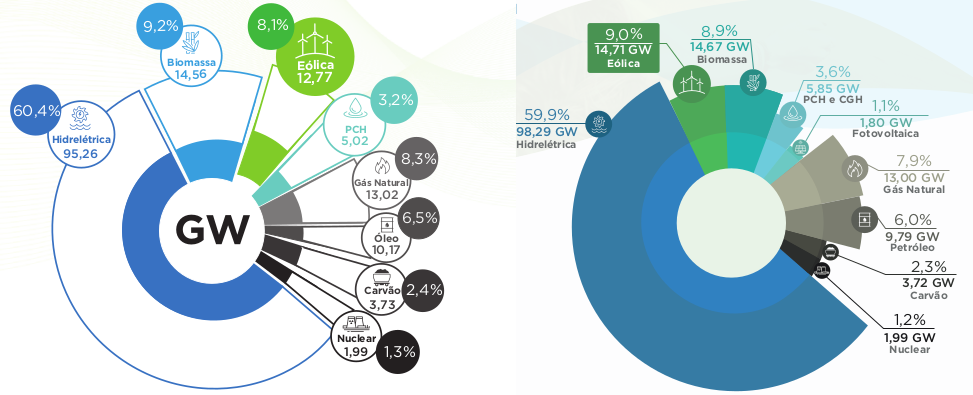
\includegraphics[width=\textwidth]{abe_2017_2018}
	\caption{Comparação entre a composição da matriz energética brasileira no ano de 2017 (esquerda) e no ano de 2018 (direita) Fonte: Boletim anual de Geração Eólica disponível em \url{http://abeeolica.org.br/dados-abeeolica}}
\end{figure}
\FloatBarrier

O Brasil conta com uma capacidade instalada de energia eólica de 12,76 GW em seus mais de 500 parques eólicos e figura mundialmente como 8º maior produtor, superando países desenvolvidos como o Canadá.

\begin{figure}[h]
    \centering
	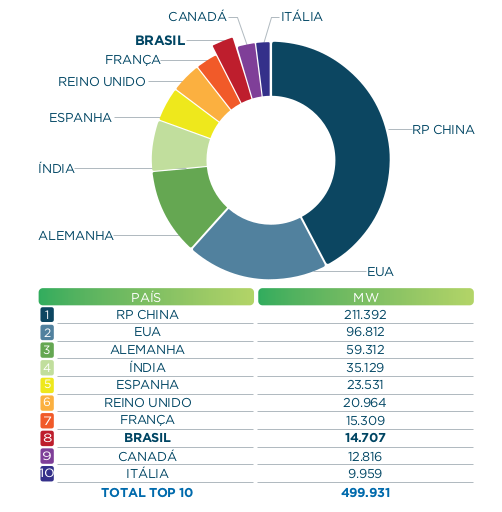
\includegraphics[scale=0.6]{abe_maiores_produtores}
	\caption{Ranking de capacidade eólica instalada acumulada. Fonte: Boletim anual de Geração Eólica disponível em \url{http://abeeolica.org.br/dados-abeeolica}}
\end{figure}
\FloatBarrier

O crescimento da captação de energia eólica no país vem crescendo constantemente, adicionando em média 2GW de capacidade instalada (máxima capacidade de produção) a cada ano desde 2013. Hoje essa fonte de energia é responsável, em média, por 11\% do abastecimento do país e 60\% do Nordeste.

\begin{figure}[h]
    \centering
	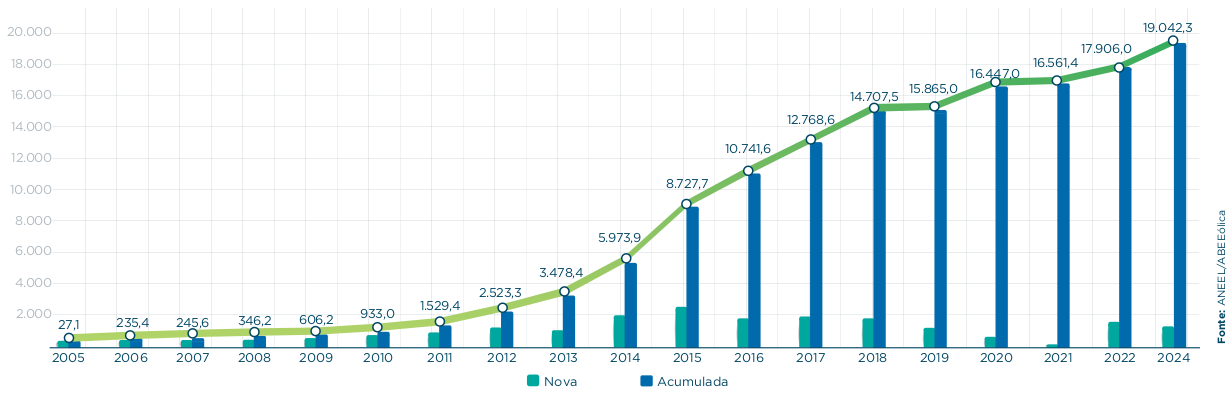
\includegraphics[width=\textwidth]{abe_evolucao_capacidade_instalada}
	\caption{Evolução da capacidade instalada de parques eólicos no Brasil. Fonte: Boletim anual de Geração Eólica disponível em \url{http://abeeolica.org.br/dados-abeeolica}} 
\end{figure}
\FloatBarrier

A principal fonte de energia elétrica do país vêm de hidrelétricas. Em períodos de estiagem, essa fonte é complementada por termoelétricas, as quais usam combustíveis fósseis para gerar energia. O seu alto custo tem impacto direto no consumidor final que paga mais pela mesma energia. 

A variabilidade do recurso eólico representa um dos maiores desafios ao seu aproveitamento. A previsão de que a maré será alta ou baixa é aceita como verdade sem mais questionamentos, enquanto que a previsão de que, devido ao movimento de massas de ar, provavelmente irá chover é encarada com forte suspeita, pois, ao contrário de outras fontes naturais de energia, tais como a energia hídrica ou solar, a energia eólica apresenta grande variabilidade \cite{thomas}, sendo, portanto, de maior dificuldade a sua previsão. Dessa forma, é de grande interesse que se entenda o seu comportamento e se desenvolva métodos para sua previsão.

% e adequado dimensionamento de recursos tanto para sua captação quanto distribuição. A construção e operação de um parque eólico é um investimento multimilionário. Dessa forma, é de suma 
%importância que o recurso eólico de um determinado local seja determinado com a maior exatidão possível e que se considere todas as restrições que possam ter qualquer efeito significativo sob tal estimativa.

% GRÁFICO DA VARIABILIDADE DAS FONTES DE ENERGIA DA BÉLGICA AQUI

% citar o meu livro de monte carlo quando mencionar estocástico ou monte carlo
% citar referência para densidade do ar
% imagem de caráter estocástico
Os principais fatores que influem na geração de energia eólica são a densidade do ar e a velocidade do vento. A potência (em watts) gerada por uma turbina é dada pela equação \cite{atlas} a qual é fornecida por fabricantes de turbinas eólicas:

\begin{equation}\label{eq:1}
	P = \frac{1}{2}\rho \frac{\pi D^2}{4}\nu^3C_p\eta
\end{equation}


\begin{flalign*}
P &= \mbox{potência elétrica na altura do cubo rotor}\left[W\right]&&\\
\rho &= \mbox{densidade do ar}\left[\frac{kg}{m^3}\right]&&\\
D &= \mbox{diâmetro do rotor}\left[m\right]&&\\\nonumber
\nu &= \mbox{velocidade do vento} \left[\frac{m}{s}\right]&&\\\nonumber
C_p &= \mbox{coeficiente aerodinâmico de potência do rotor}\left[W\right]&&\\\nonumber
\eta &= \mbox{eficiência do conjunto gerador/transmissão}&&\\\nonumber
\end{flalign*}

O fato de a potência variar com o cubo da velocidade do vento evidencia a importância da determinação precisa dessa grandeza.

A conversão entre velocidade e potência é feita por uma curva de potência fornecida pelo fabricante da turbina utilizada. Ela representa a potência que seria gerada para cada velocidade incidente perpendicularmente às pás da turbina. Uma vez feita a previsão da velocidade do vento utilizar-se-a, neste trabalho, uma curva de potência genérica como a exibida abaixo para obter a previsão em energia ao invés de velocidade do vento. Observa-se que baixas velocidades de vento resultam em baixa produção de energia e que a velocidades muito altas a produção é constante. Para velocidades muito intensas a turbina é temporariamente desligada para evitar danos estruturais.

% sob as condições às quais a turbina fora exposta para medição da curva de potência

\begin{figure}[h]
    \centering
	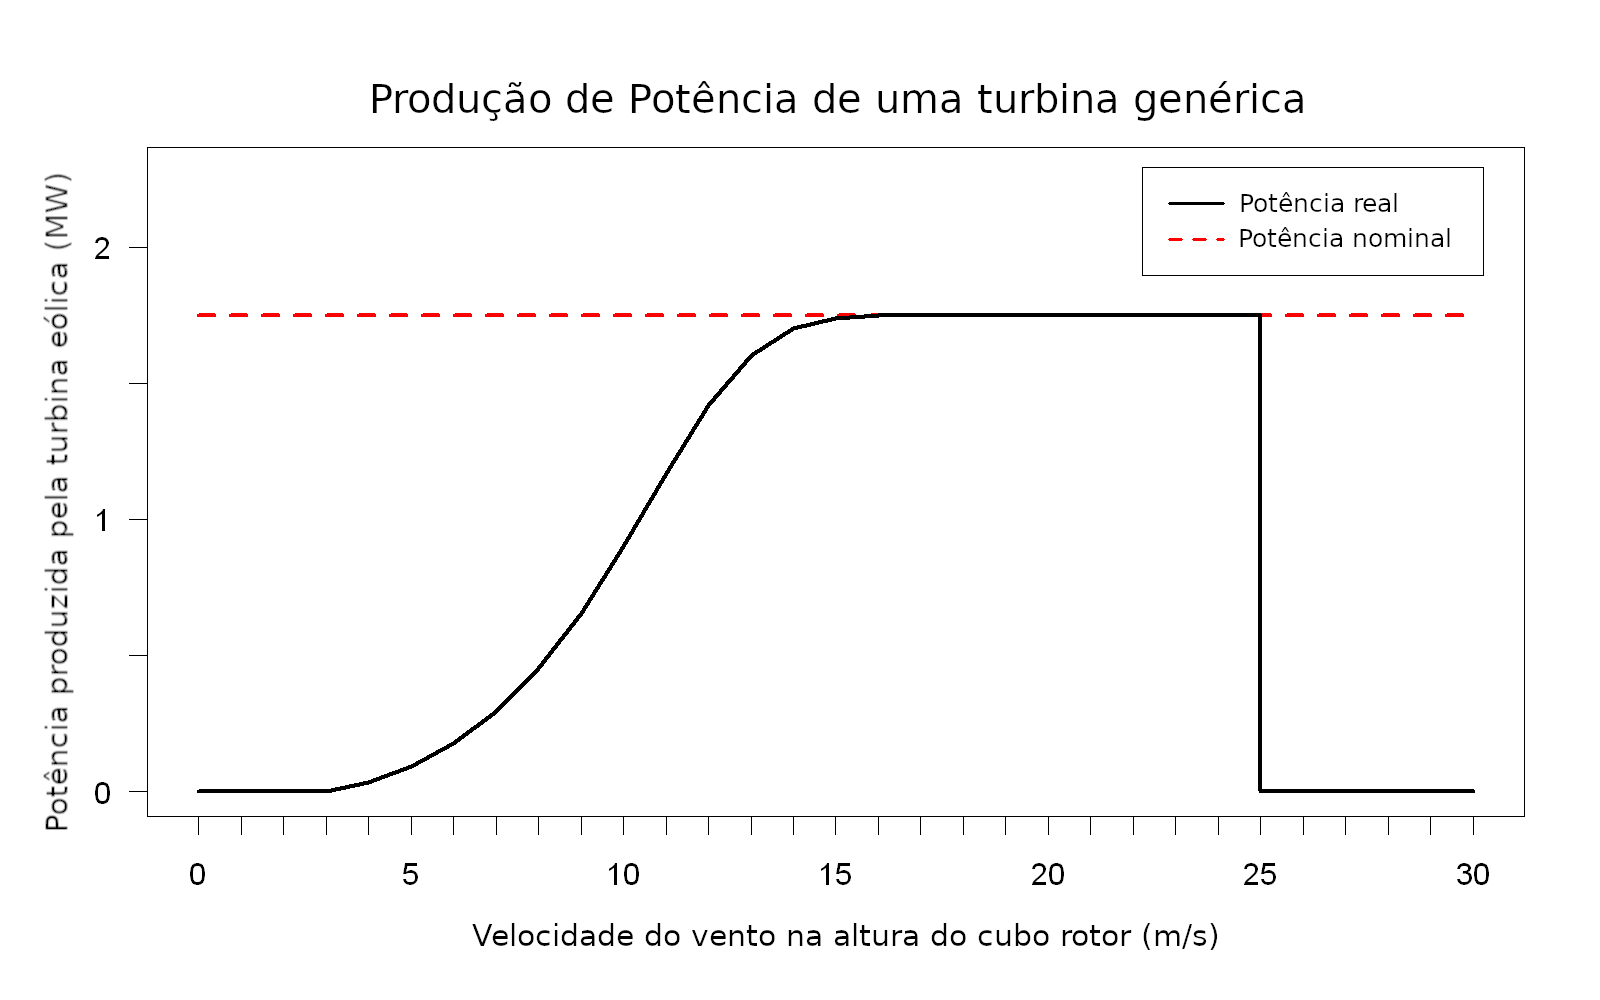
\includegraphics[width=\textwidth]{powercurve}
	\caption{Curva de potência de uma turbina genérica. Adaptado de \url{https://upload.wikimedia.org/wikipedia/commons/6/67/Powercurve.png}}
\end{figure}
\FloatBarrier

Na equação \ref{eq:1}, exceto pela velocidade do vento, os demais parâmetros são controlados ou apresentam pouca variabilidade como a densidade do ar, por exemplo, que é relativamente constante para um dado macroclima. A velocidade do vento, por outro lado, tem caráter fortemente estocástico, ou seja, seu comportamento esta associado a um processo aleatório. A sua previsão demanda o uso de modelos matemáticos que levem em conta tal comportamento.

Fenômenos estocásticos são comuns na natureza: o movimento errático que uma partícula macroscópica sofre ao ser 
imersa num fluído (composto por partículas microscópicas) conhecido como movimento Browniano; o decaimento radioativo de átomos em que não se sabe em qual momento dado átomo emitirá radiação (conhece-se apenas uma taxa característica de emissão). 

Exemplos associados a atividade humana também são comuns sendo a evolução temporal do valor de ativos econômicos o exemplo mais marcante e para cujo entendimento se desenvolveu um arcabouço matemático sofisticado. Esse conhecimento pode ser utilizado para estudar quaisquer outros fenômenos estocásticos. A imagem traz dois exemplos de séries estocásticas: uma série de dados de vento (esquerda) e uma série de dados financeira (direita). Os métodos desenvolvidos para estudar séries financeiras podem ser usado com sucesso para séries de velocidade do vento.

\begin{figure}[h]
    \centering
	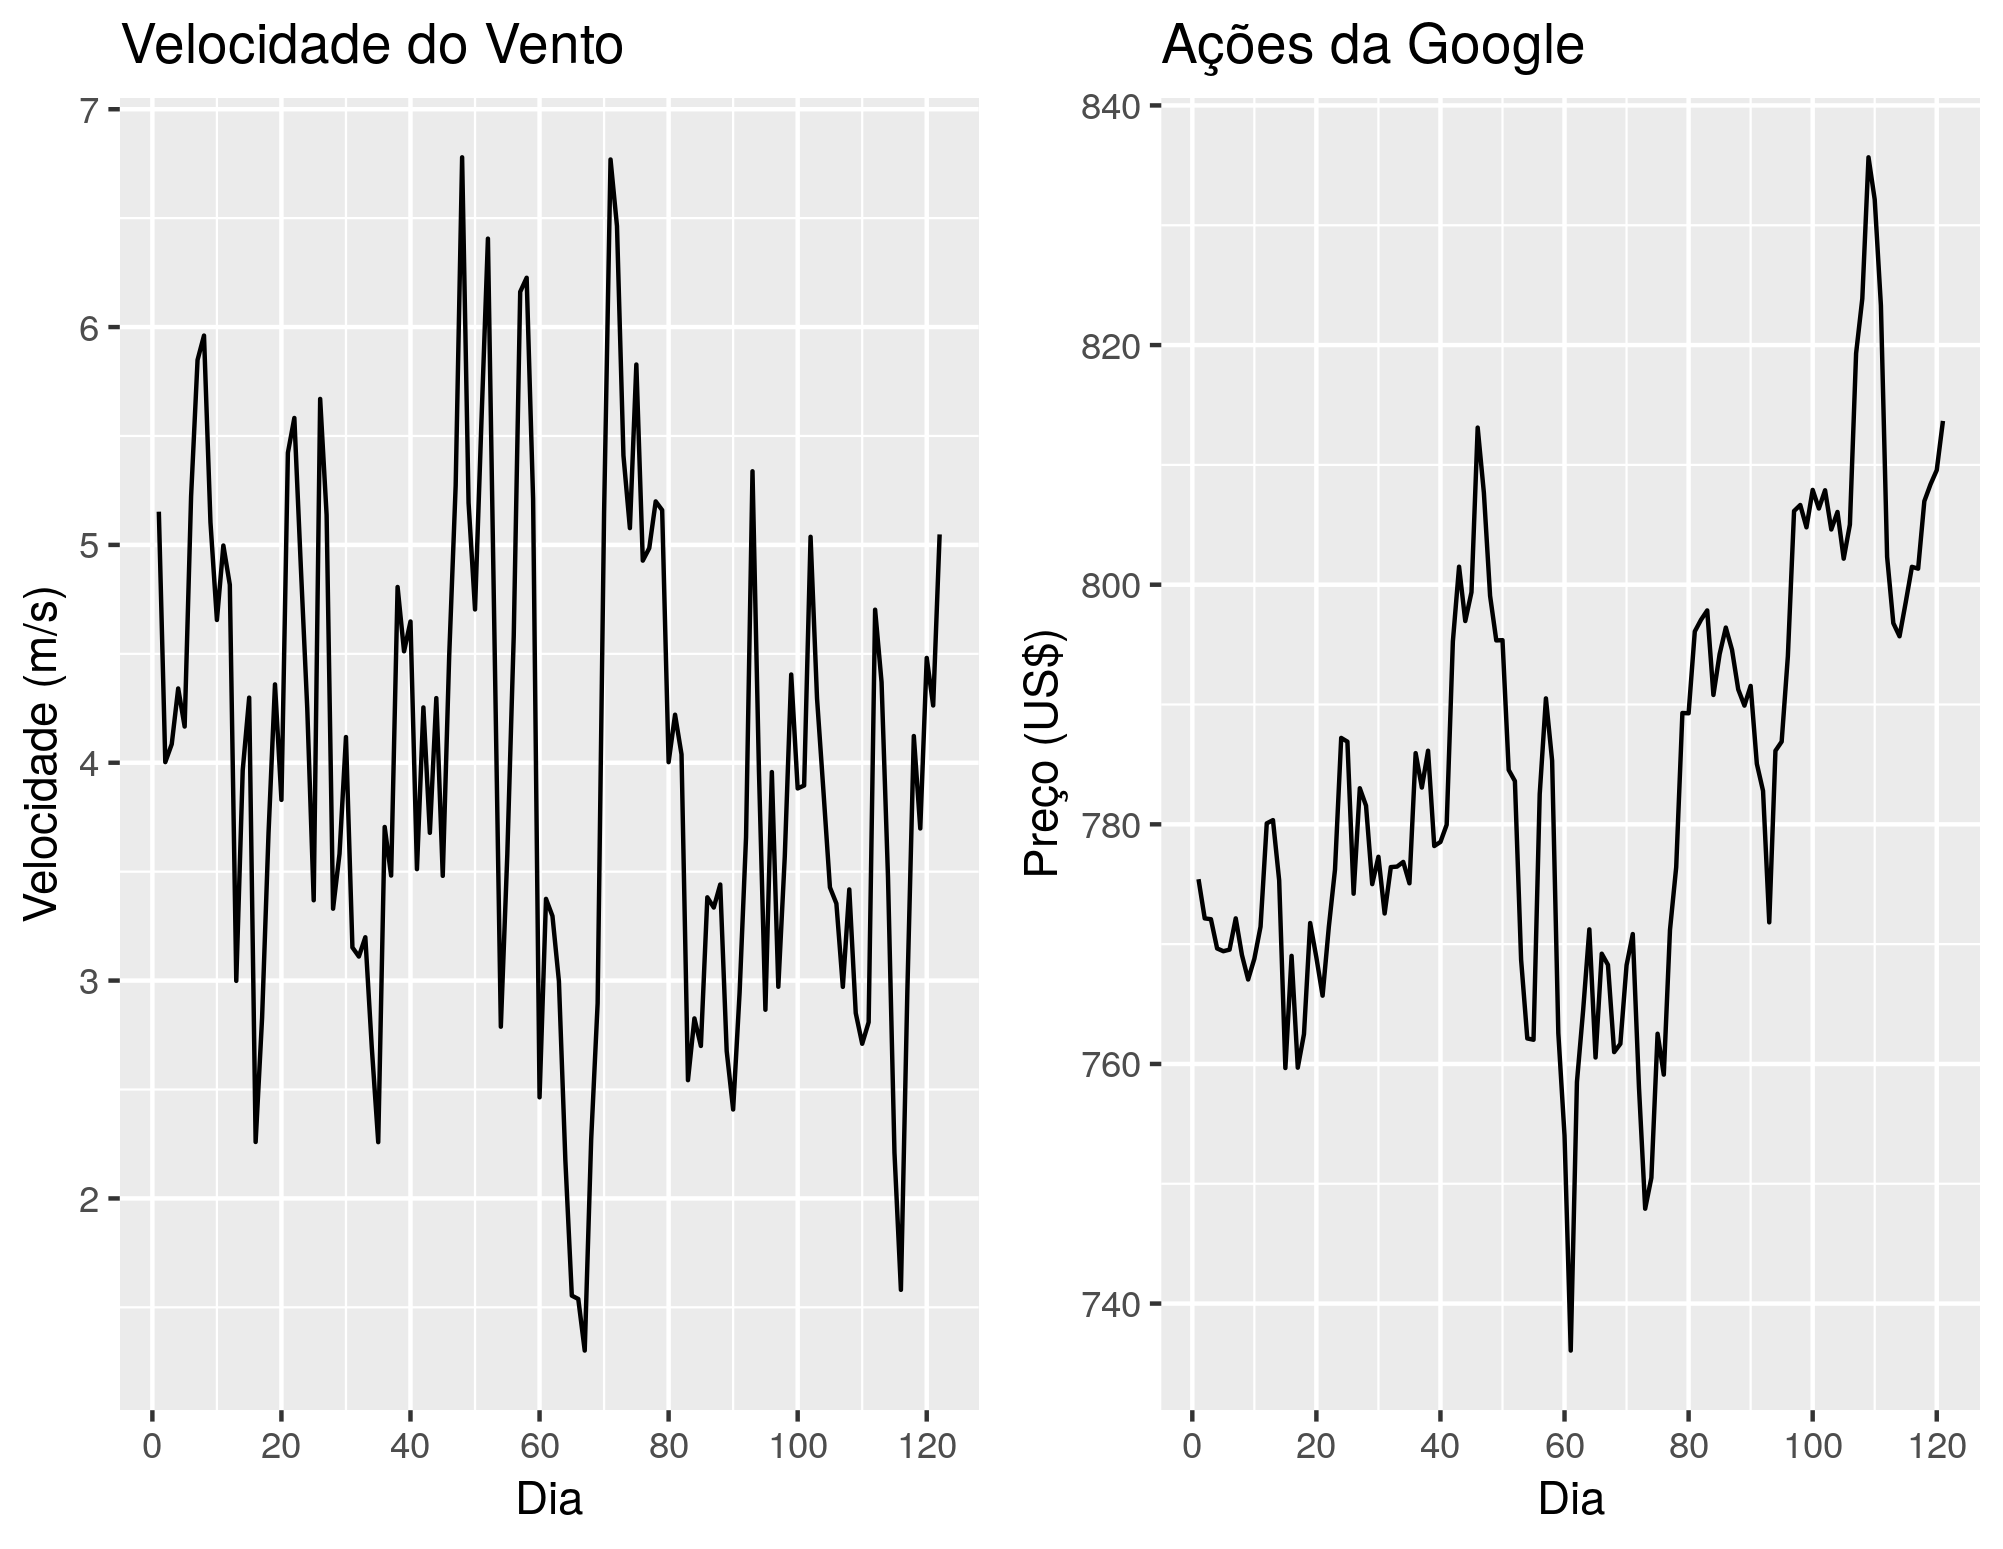
\includegraphics[width=\textwidth]{wind_money}
	\caption{À esquerda velocidade do vento em m/s para uma região no sul do Ceará e à direita o preço de fechamento das ações da google para 120 dias de 2013. Baseado na série de dados ERA5 da \cite{era5} e NASDAQ disponível em \url{https://www.nasdaq.com/symbol/goog}.}
\end{figure}
\FloatBarrier

Yule e Walker \cite{yulewalker} propuseram a representação de uma grandeza estocástica pelo resultado de choques aleatórios descritos por um filtro linear aplicado em ruído branco:

$$ v_{t} = \mu + a_t + \psi_{1}a_{t-1} + \psi_{2}a_{t-2} + \dots $$

Essa ideia dá origem a modelos autorregressivos que descrevem a estrutura de séries temporais levando em conta termos anteriores da própria série. Box e Jenkins \cite{boxjay} descrevem esse método como "deixar que os dados falem por eles próprios", ou seja, nenhuma variável exógena é empregada, apenas a própria série. Esse método tem sido empregado com sucesso para prever o comportamento futuro de séries temporais em diversas áreas. Diversas variações do modelo original foram desenvolvidas ao longo dos anos. O conjunto de todas essas variações são denominadas modelos ARIMA, um acrônimo do inglês \textit{autoregressive integrated moving average}, que significa modelo autorregressivo (AR) integrado (I) de média móvel (MA).

%Um modelo que combina tanto um caráter autogressivo quanto de média móvel pode ser descrito da seguinte forma:
%$$ y^{'}_{t} = c + \phi_{1}y^{'}_{t-1} + \dots + \phi_{p}y^{'}_{t-p} + \theta_{1}\varepsilon_{t-1} + \dots + \theta_{q}\varepsilon_{t-q} + \varepsilon_{t}$$

\cleardoublepage
\part{Estudo de caso}

\chapter{Caracterização da região}

De modo a desenvolver as ideias desse trabalho escolheu-se arbitrariamente uma região localizada no estado do Ceará. Optou-se pela região nordeste por ser a região onde há mais investimentos em energia eólica e que responde pela maioria dos parques em operação no país. Os métodos desenvolvidos são, no entanto, aplicáveis a qualquer região, pois têm como entrada apenas uma série temporal.

A região de interesse encontra-se numa chapada elevada, um local com topografia muito favorável a instalação de um parque eólico. Sabe-se da dinâmica de fluídos que o escoamento é acelerado quando exposto a um diferencial de elevação. Na imagem abaixo pode-se perceber o quão elevada a chapada é em relação ao seu redor.

\begin{figure}[h]
    \centering
	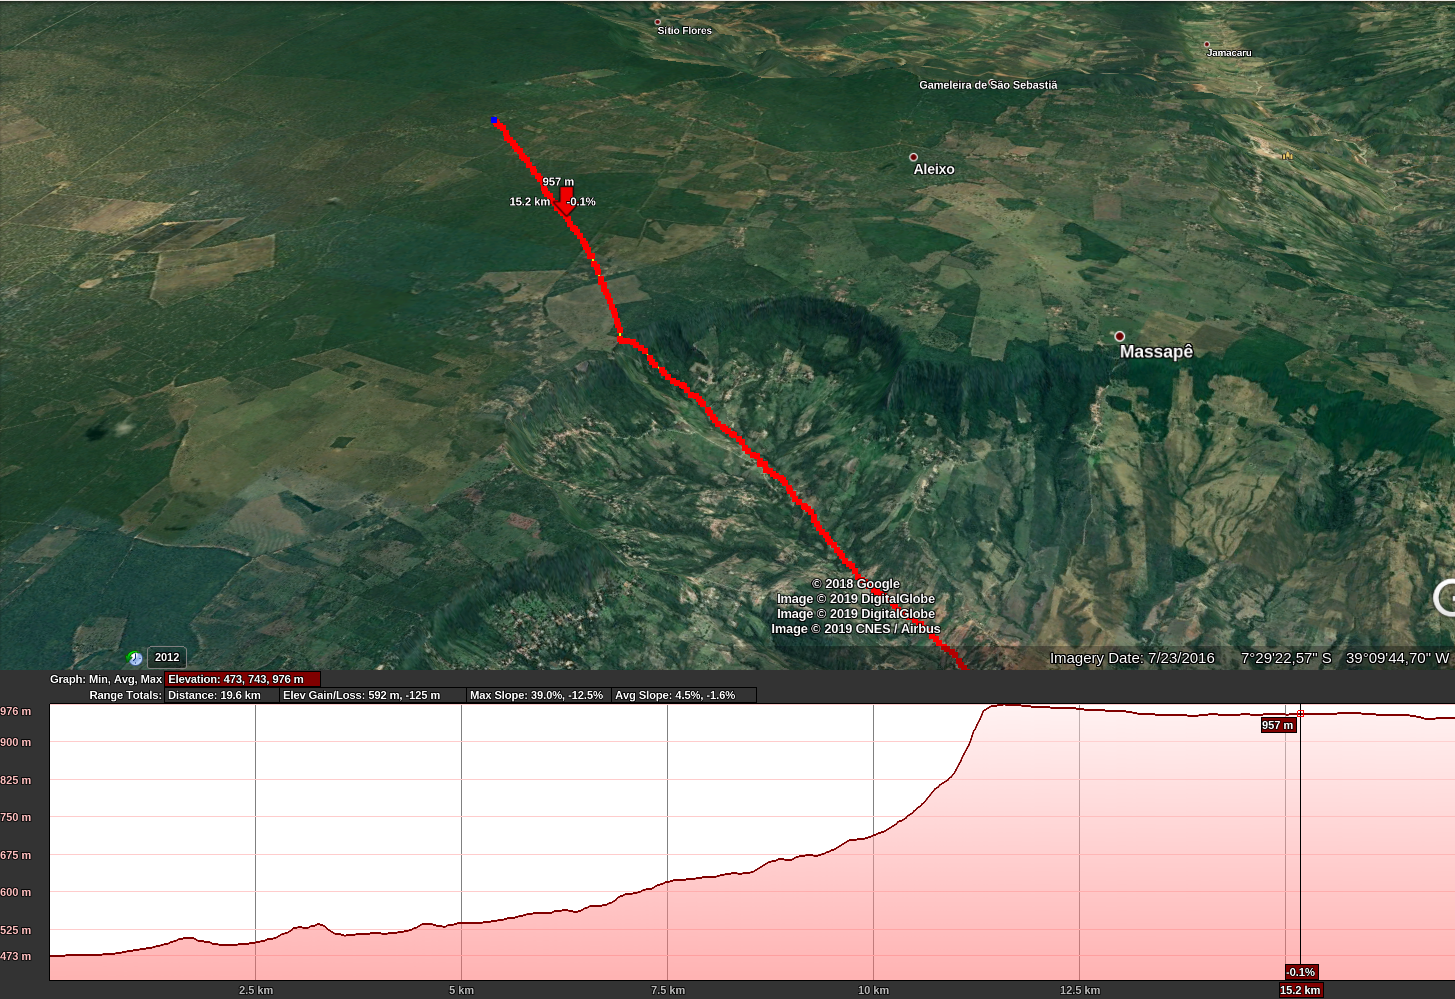
\includegraphics[width=\textwidth]{elevation2}
	\caption{Variação da elevação na direção preferencial de escoamento do vento.\newline Google earth V 7.3.2.5776. (23 de Julho, 2016). Rio Grande do Sul, Brasil. \ang{7} 29\textquotesingle\ 22,57\textquotesingle\textquotesingle\ S, \ang{39} 09\textquotesingle\ 44,70\textquotesingle\textquotesingle\ W, Eye alt 205,32 km.}
\end{figure}
\FloatBarrier

Detalhes da topografia da região podem ser visualizados na imagem abaixo a qual exibe em detalhes a elevação por meio de linhas de contorno além dos declives e a rosa dos ventos.

\begin{figure}[h]
    \centering
	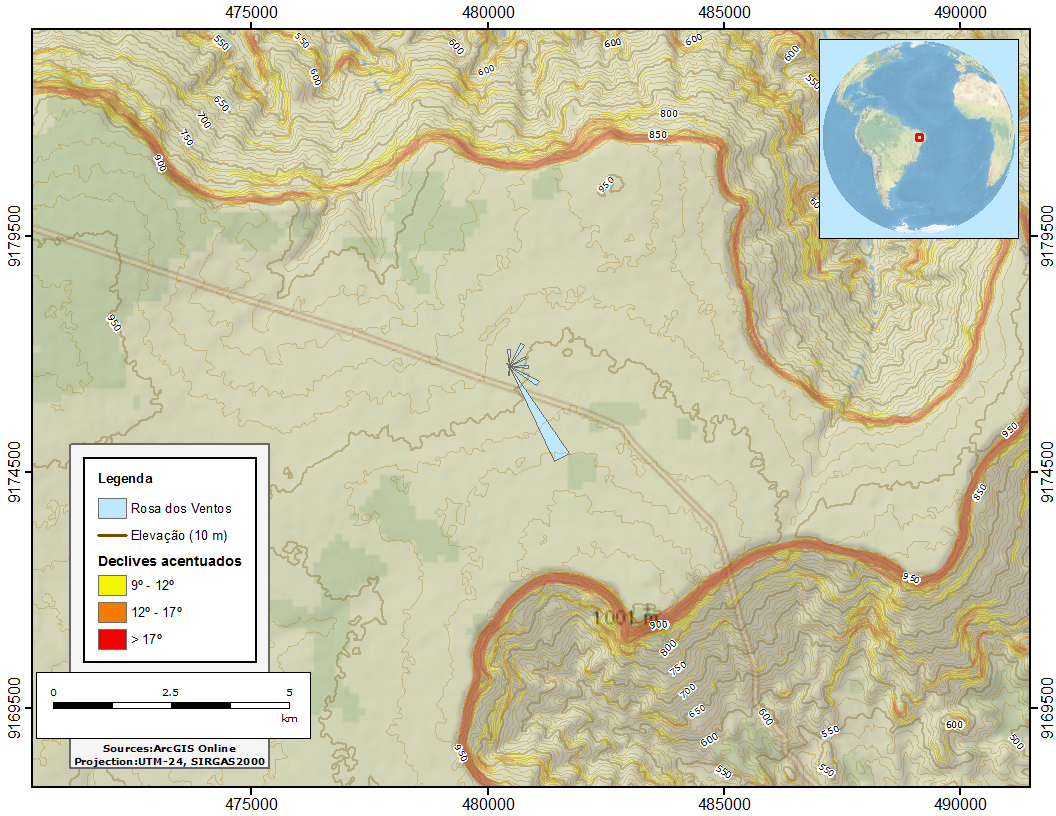
\includegraphics[width=\textwidth]{arcmap}
	\caption{Topografia da região de interesse. Baseado na série de dados SRTM disponíveis em \url{https://earthdata.nasa.gov}.}
\end{figure}
\FloatBarrier

Na camada da atmosfera próxima ao solo, a velocidade do vento aumenta com a altura conforme uma lei de potência empírica:

\begin{equation}
\frac{v}{v_r} = \left(\frac{h}{h_r}\right)^\alpha
\end{equation}

\begin{flalign*}
v &= \mbox{velocidade do vento à altura } h&&\\
v_r &= \mbox{velocidade do vento à altura de referência } h_r&&\\\nonumber
\alpha &= \mbox{coeficiente de cisalhamento, parâmetro estimado a partir dos dados}&&\\\nonumber 
\end{flalign*}

Em suma, a partir da imagem acima, é possível determinar as melhores posições para se colocar turbinas de um parque eólico:
\begin{itemize}
\item Na chapada, onde a velocidade do vento é maior devido a sua elevação de acordo com a lei de potência;
\item Nas zonas de baixa declividade para facilitar as simulações computacionais;
\item Nas bordas devido ao diferencial de elevação que causa aceleração do vento;
\item Orientadas a aproximadamente 150º em relação do norte verdadeiro de modo a captar o vento oriundo de sua direção preferencial.
\end{itemize}

\chapter{A série temporal modelo}\label{modelo}

Para exemplificar a elaboração do modelo proposto, utilizou-se uma série de dados disponibilizada publicamente pela organização européia ECWMF. Essa série conta com uma vasta gama de grandezas físicas medidas por satélite oriundas de diversas fontes. Esses dados são agregados e tratados de modo a melhorar sua qualidade. Existem diversas outras séries de dados de satélite com o mesmo propósito, tal como a série ERA-Interim (antecessora da ERA 5) ou as séries MERRA e MERRA 2 produzidas pela NASA. No entanto, observa-se que a qualidade da fonte ERA 5 é muito superior. Isso é empiricamente constatado devido a excelente correlação com dados de torres de medição instaladas no solo. Essa melhoria deve-se tanto a melhorias técnicas na assimilação e agregação de dados quanto a maior resolução espacial da série ERA 5: enquanto MERRA e MERRA 2 apresentam uma resolução espacial de 50 km em latitude e longitude, ERA 5 apresenta 30 km. 

A grandeza de interesse para esse trabalho é a velocidade do vento a 100 m de altura em relação ao solo. Essa é a altura disponibilizada pela fonte ERA 5. Outras alturas estão disponíveis, mas são obtidas por interpolação e portanto são de qualidade inferior. Essa é uma altura adequada pois a altura do cubo rotor de aerogeradores comerciais varia tipicamente entre 80 m e 130 m. 

%Quando necessário as previsões de velocidade podem ser extrapoladas verticalmente por meio de uma lei de potência

A série ERA 5, assim como as outras mencionadas, possuem dados para todo o globo, dividindo-o em uma rede de nós com resolução de 30 km x 30 km em latitude e longitude, respectivamente. A imagem abaixo exemplifica como esses nós são dispostos na região de interesse. 

%A região nordeste é muito atrativa para construção de parques eólicos devido a alta velocidade média do vento. 

\begin{figure}[h]
    \centering
	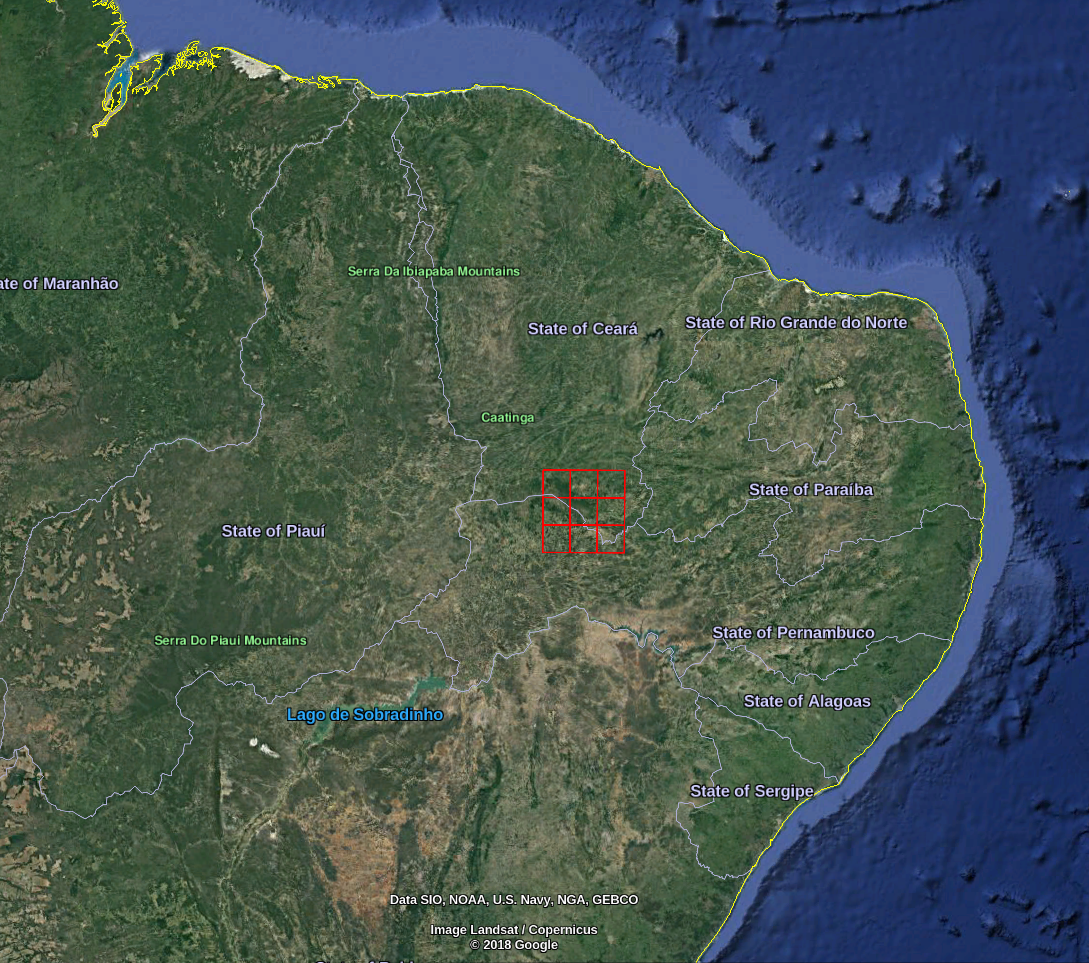
\includegraphics[width=\textwidth]{era5nodes}
	\caption{Alguns nós da série ERA 5 ao sul do Ceará, Brasil.\newline Google earth V 7.3.2.5776. (14 de Dezembro, 2015). Rio Grande do Sul, Brasil.
\ang{7} 14\textquotesingle\ 11,54\textquotesingle\textquotesingle\ S, \ang{40} 04\textquotesingle\ 12,31\textquotesingle\textquotesingle\ W, Eye alt 1808,45 km.}
\end{figure}
\FloatBarrier

Cada nó cobre uma vasta região. A velocidade reportada para cada nó é uma média das velocidades da respectiva região. A campanha de medição necessária que antecede a construção de um parque eólico exige a instalação de torres de medição no local. Desse modo, a resolução dessas medições é muito maior do que a oferecida pela série ERA 5. No entanto, os dados de medições de torres não são disponibilizados publicamente. Com base na excelente correlação entre as séries ERA 5 e séries medidas por torres de projetos, acredita-se que o procedimento exposto neste trabalho possa ser aplicado com sucesso em dados medidos por torres em solo ou na nacele dos próprios aerogeradores.

%de tal modo que dados de velocidade do vento, coletados continuamente, .


Os dados são fornecidos em base horária e compreendem o período de Janeiro de 2000 a Janeiro de 2019. 

\chapter{Caracterização dos dados}

O começo de qualquer análise de séries temporais se dá pelo gráfico dos valores que assume ao longo do tempo. Por meio desse gráfico, é possível identificar qualitativamente tendências, sazonalidade, ciclicidade, valores atípicos, caráter estacionário e comportamento da variância:

\begin{figure}[h]
    \centering
	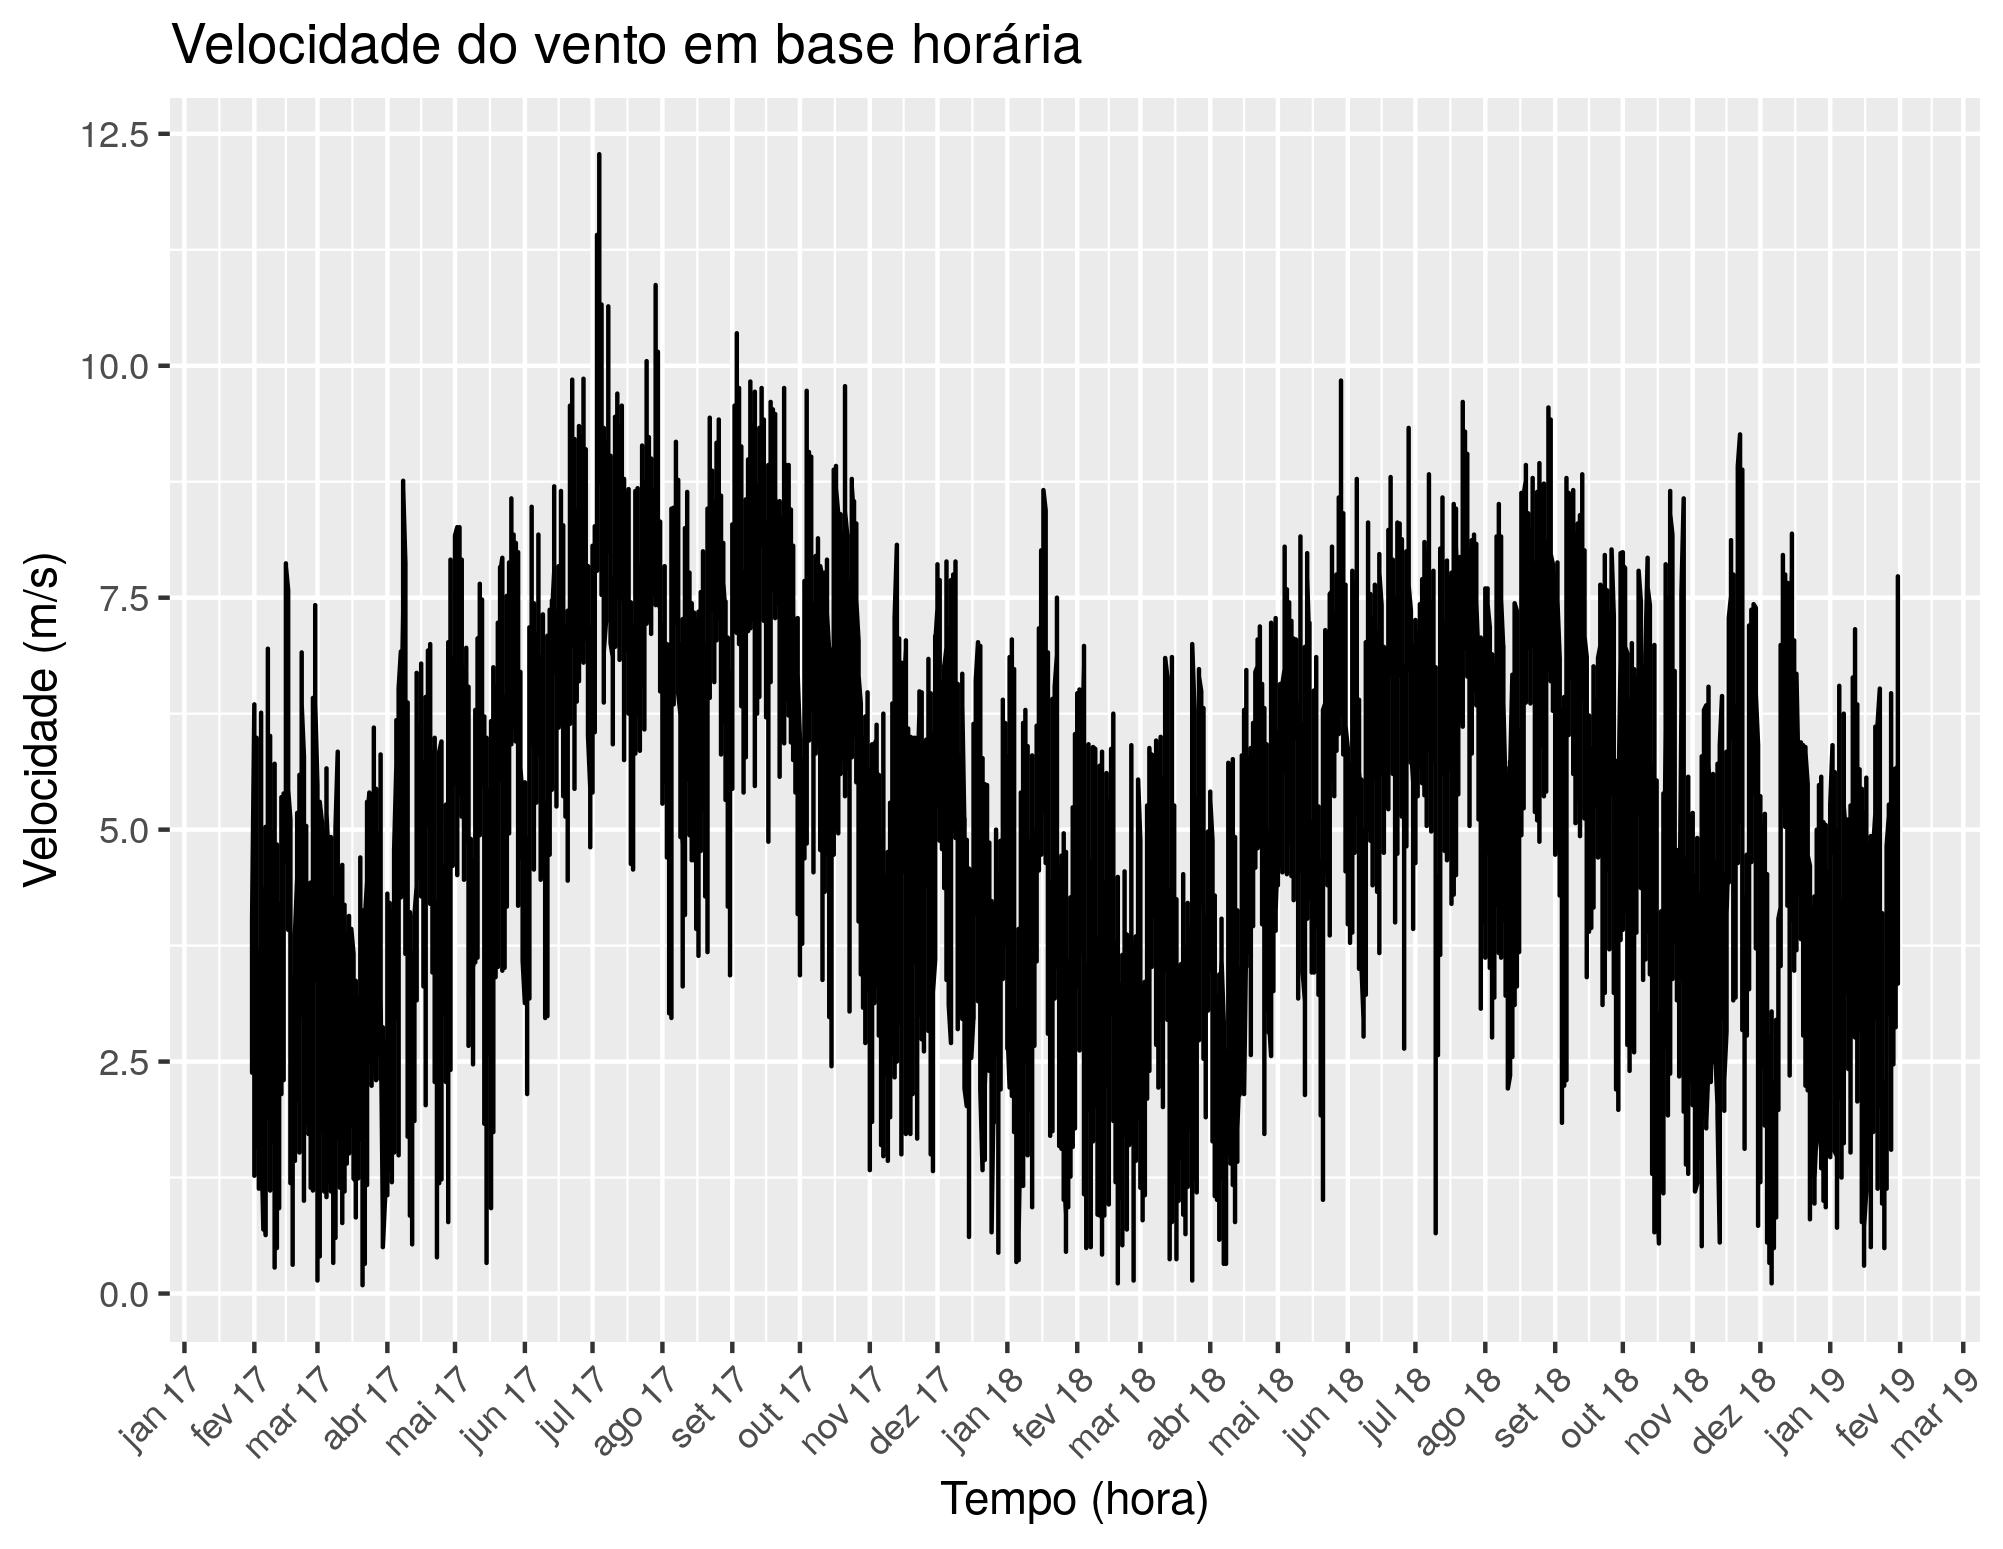
\includegraphics[width=\textwidth]{entire_series_hourly_basis.png}
	\caption{Velocidade do vento registrada por satélite na região de interesse nos anos de 2017 e 2018. Baseado na série de dados ERA5 da \cite{era5}.}
\end{figure}
\FloatBarrier

Apenas pela análise visual é possível perceber que a velocidade tem máximos nos meses de inverno e mínimos nos de verão, que há sazonalidade anual. A série não aparenta ter deriva, oscila ao longo de um valor médio. Por apresentar sazonalidade a série não é estacionária. Como os métodos apresentados neste trabalho tomam como premissa que a série de entrada é estacionária, é necessário transformá-la previamente em uma série estacionária e ser capaz de fazer o caminho reverso após a sua previsão. Nessa escala não é possível afirmar algo conclusivo sobre a variância da série.

\section{Distribuição de probabilidades}

O histograma de velocidades exibido abaixo indica que a série não segue uma distribuição normal e que uma distribuição de cauda longa à direita seria mais adequada. 

\begin{figure}[h]
    \centering
	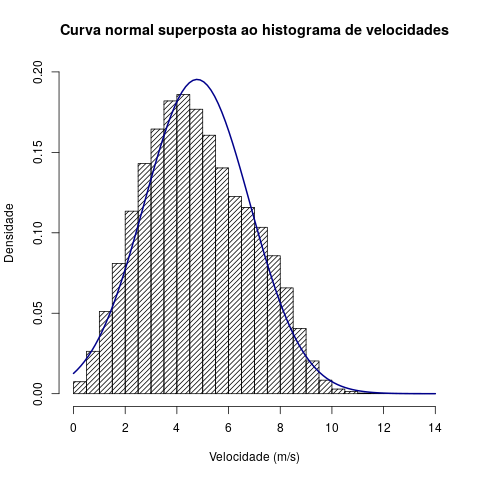
\includegraphics[scale=0.7]{normal_overlay}
	\caption{Histograma de velocidades do nó noroeste da série de dados modelo. Baseado na série de dados ERA5 da \cite{era5}.}
\end{figure}
\FloatBarrier

Por meio do gráfico de Cullen e Frey \cite{frey} é possível afirmar que a distribuição de probabilidades que melhor descreve os dados se aproxima de uma distribuição beta:

\begin{figure}[h]
    \centering
	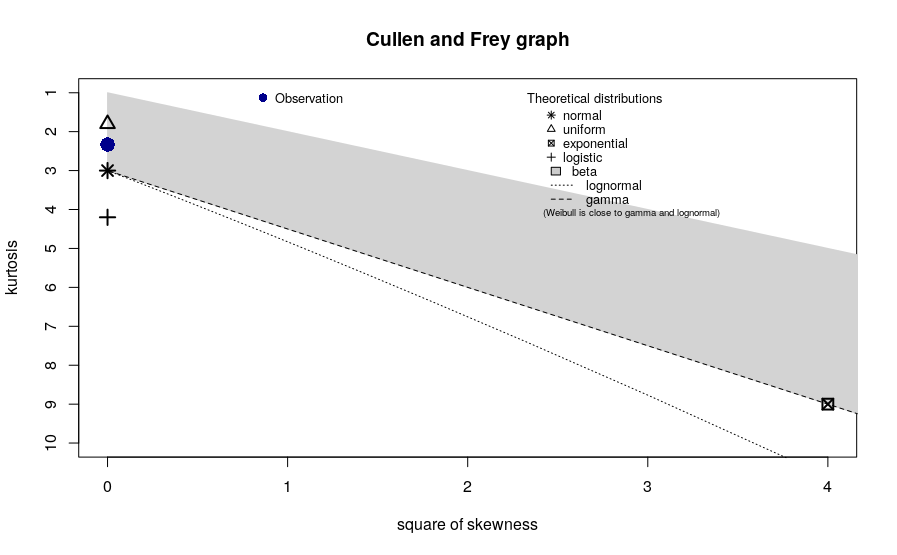
\includegraphics[scale=0.6]{cullen}
	\caption{Gráfico de Cullen e Frey para os dados do nó noroeste da série de dados modelo. Baseado na série de dados ERA5 da \cite{era5}.}
	\label{fig:cullen}
\end{figure}
\FloatBarrier

Esse gráfico utiliza momentos de ordem mais alta, curtose (ordenada) e quadrado da assimetria (abscissa), para identificar desvios da distribuição normal (curtose igual 3 e assimetria igual a 0) e indicar qual classe de distribuição melhor ajuste os dados de entrada.

\section{Direção}

A direção do vento é um fator importante para a conversão de velocidade do vento em energia. A orientação paralela a direção preferencial do vento garante maior energia rotacional nas pás. No entanto, em excesso pode danificar alguns componentes das turbinas tais como rolamentos. Aerogeradores comerciais contam com estratégias de parada sob ventos excessivos ou sob turbulência excessiva de aerogeradores próximos.
Um modo claro de representar o comportamento da direção do vento é pela rosa dos ventos, exibida abaixo para um nó da série modelo:

\begin{figure}[h]
    \centering
	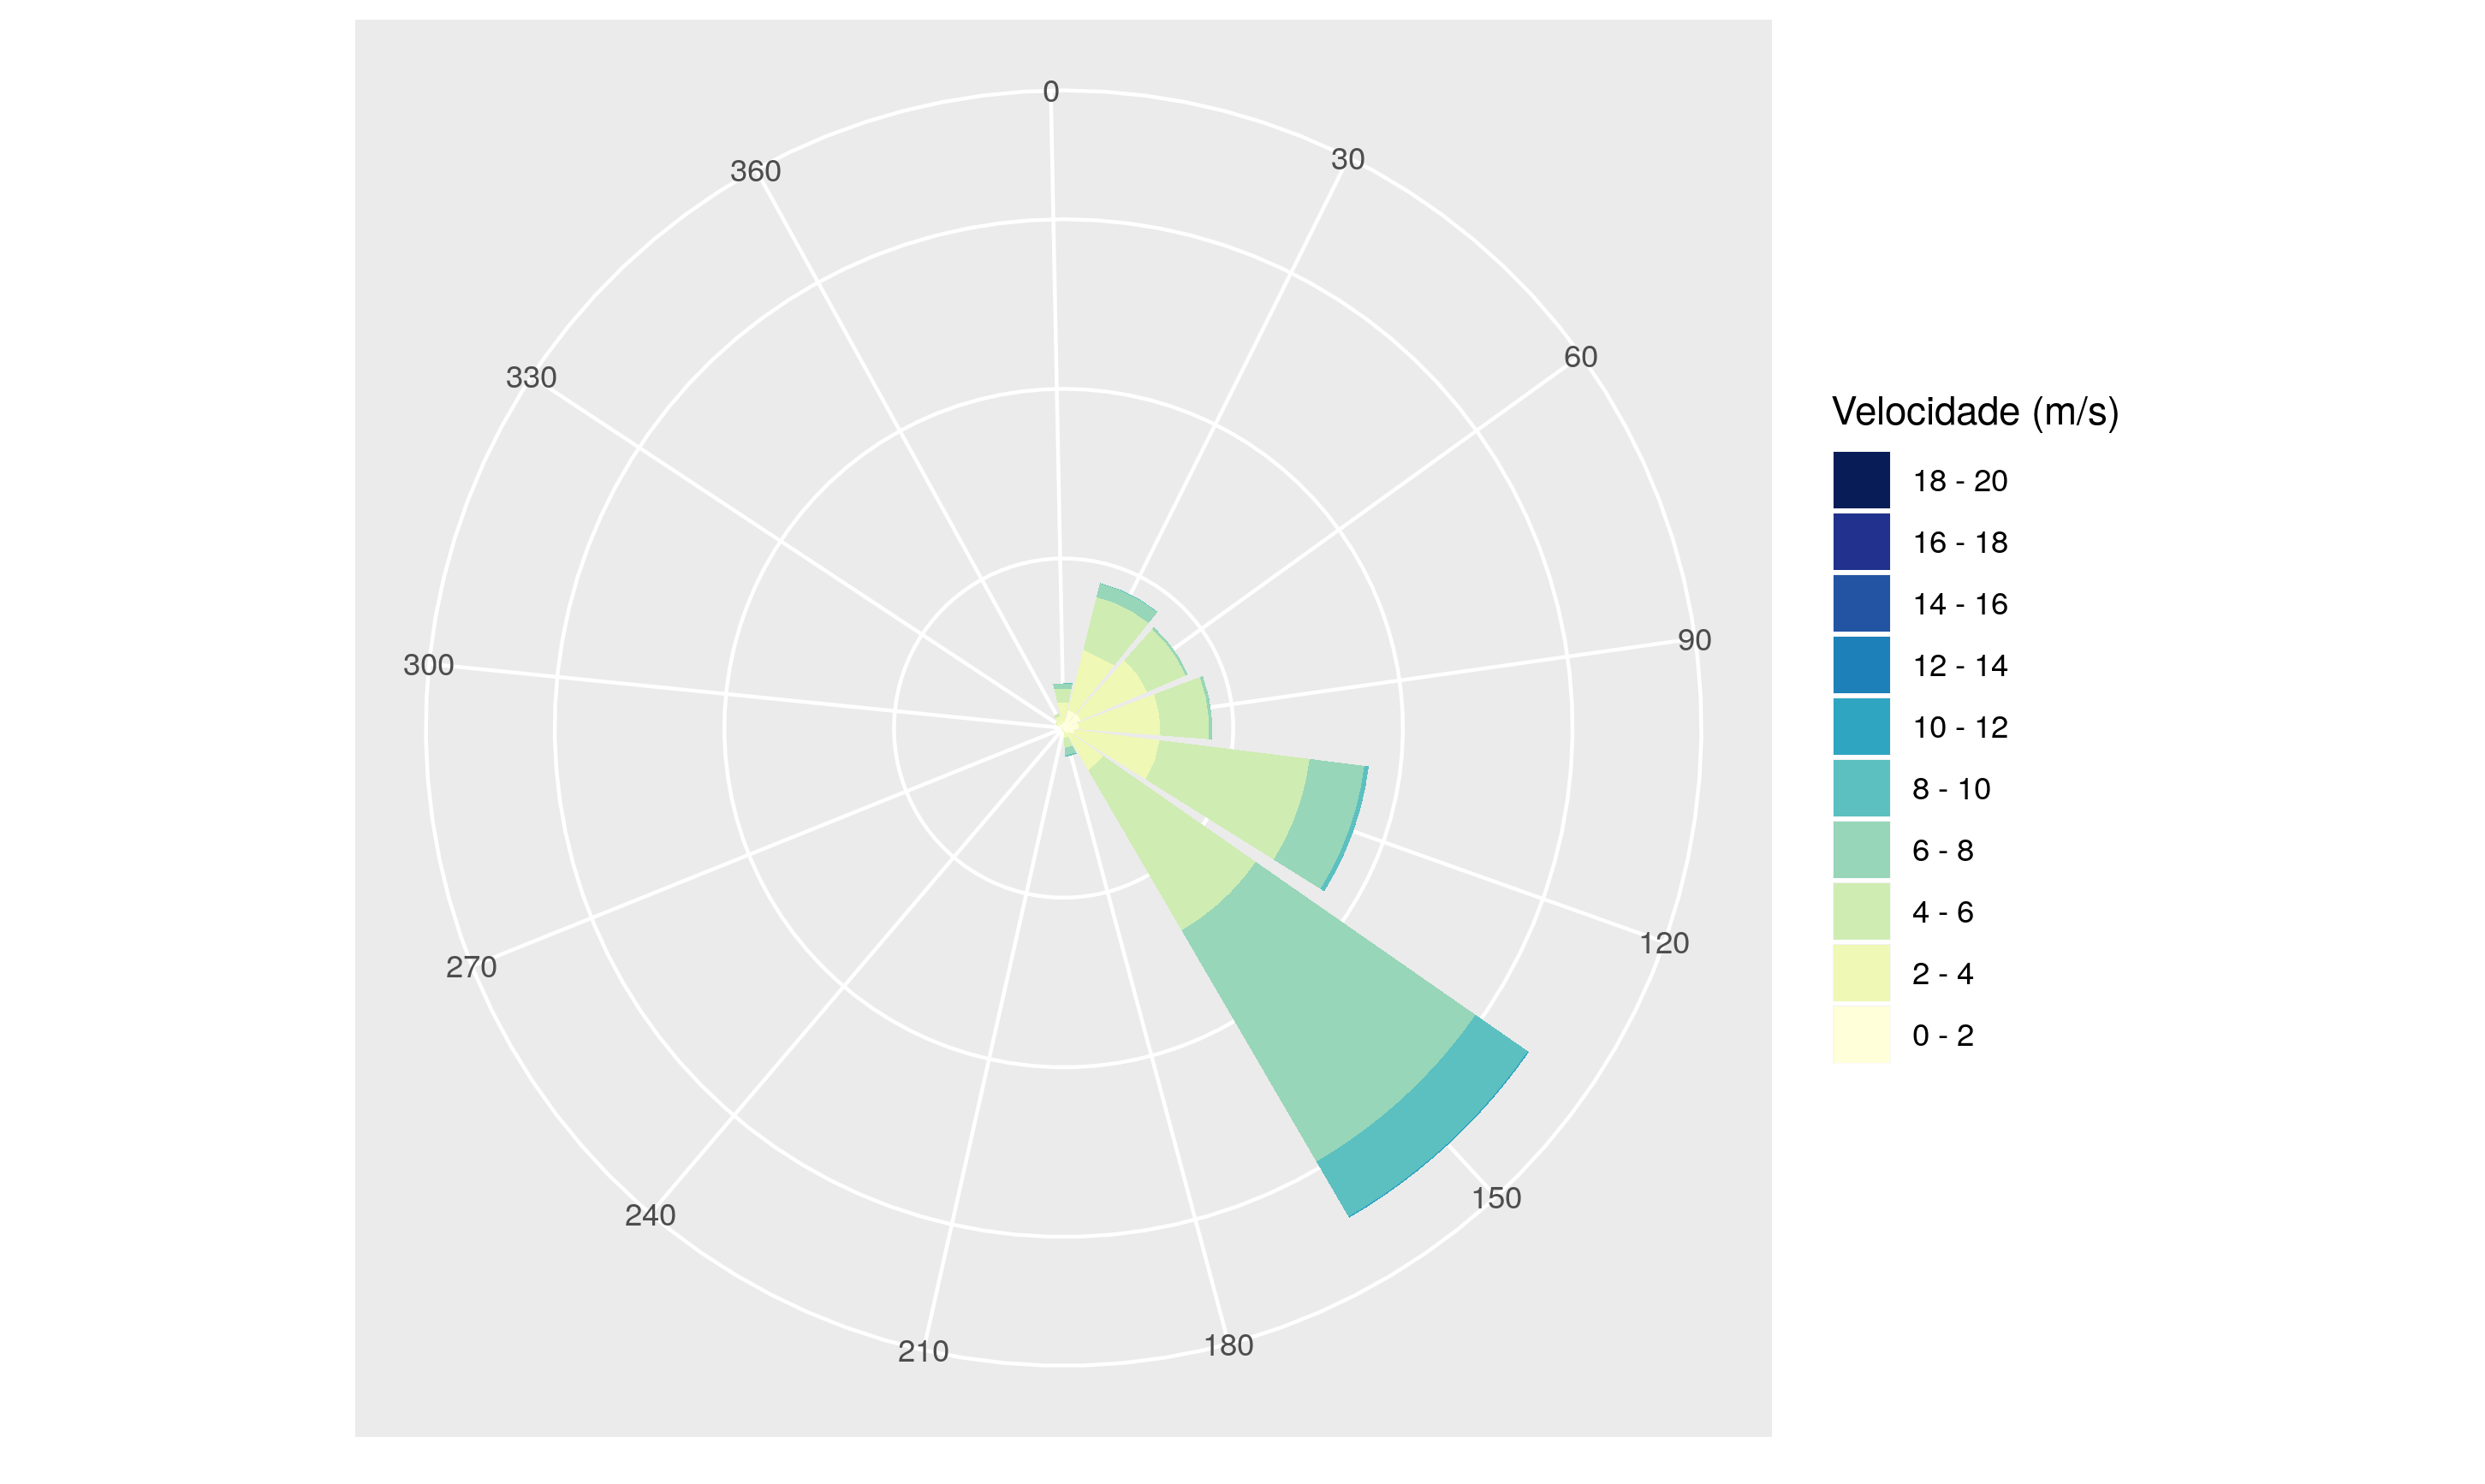
\includegraphics[width=\textwidth]{windrose}
	\caption{Rosa dos ventos do nó noroeste da série ERA5 para a região de interesse. Baseado na série de dados ERA5 da \cite{era5}.}
	\label{fig:windrose}
\end{figure}
\FloatBarrier

\section{Sazonalidade}

O caráter sazonal da velocidade do vento pode ser investigado sob diferentes perspectivas. 

\begin{figure}[h]
    \centering
	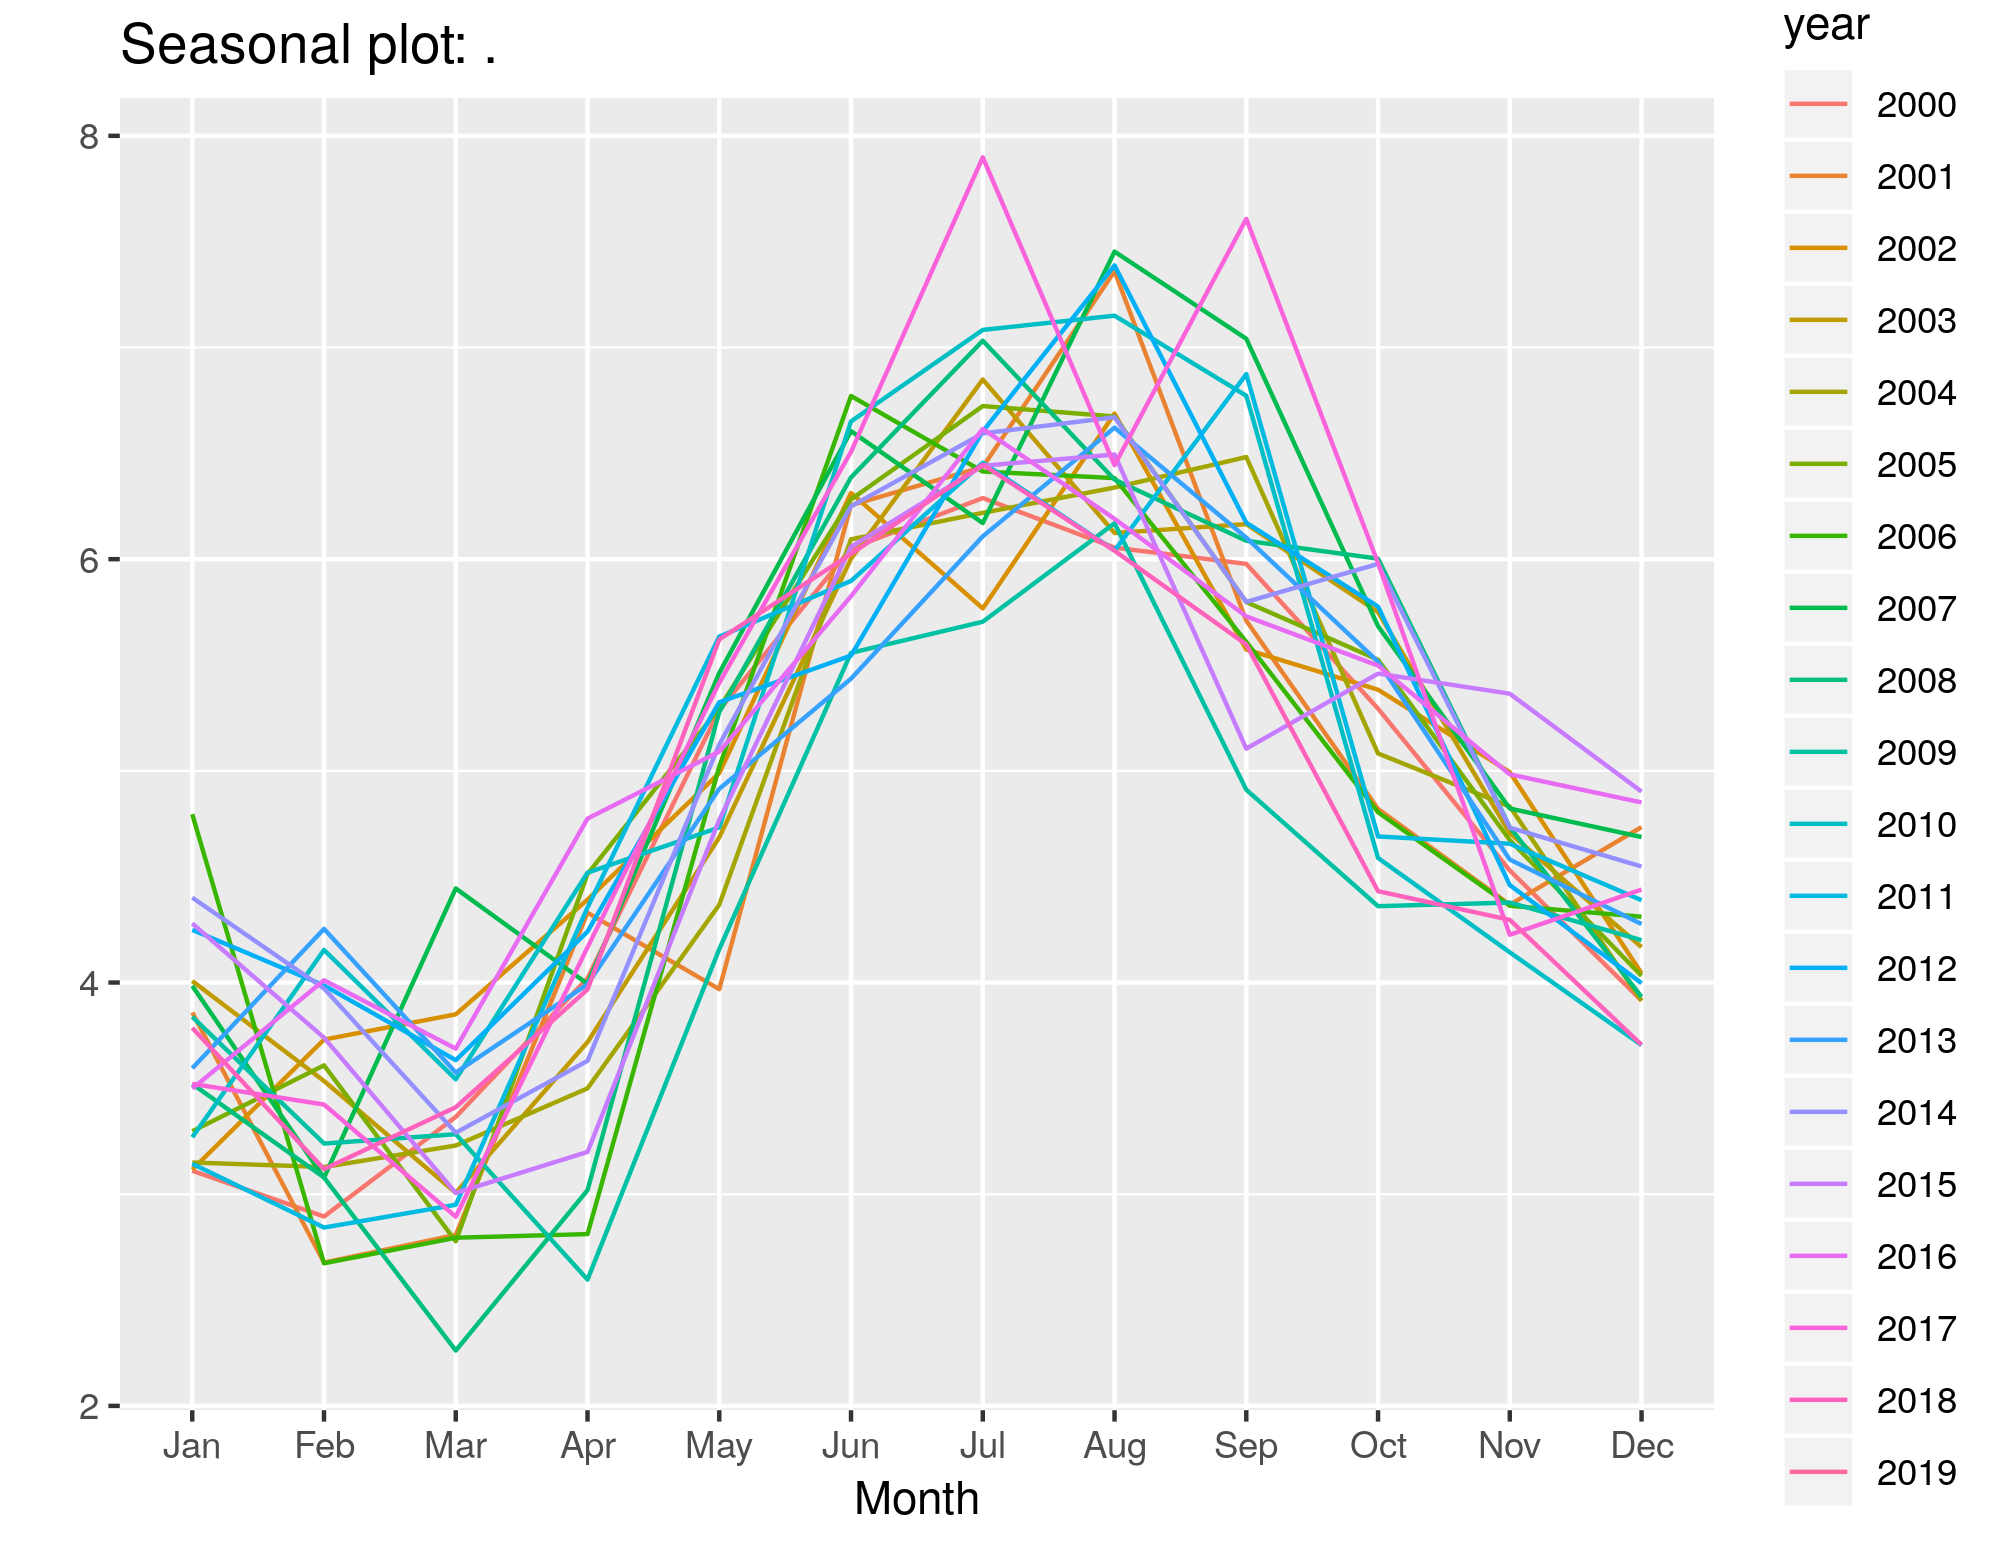
\includegraphics[width=\textwidth]{season_plot}
	\caption{Velocidade média (m/s) para cada mês do ano. Cada curva representa algum ano entre 2000 e 2019. Baseado na série de dados ERA5 da \cite{era5}.}
\end{figure}
\FloatBarrier

O gráfico acima deixa claro que existe um padrão anual. Para todos os anos da série a velocidade mensal tem um comportamento muito similar.

\begin{figure}[h]
    \centering
	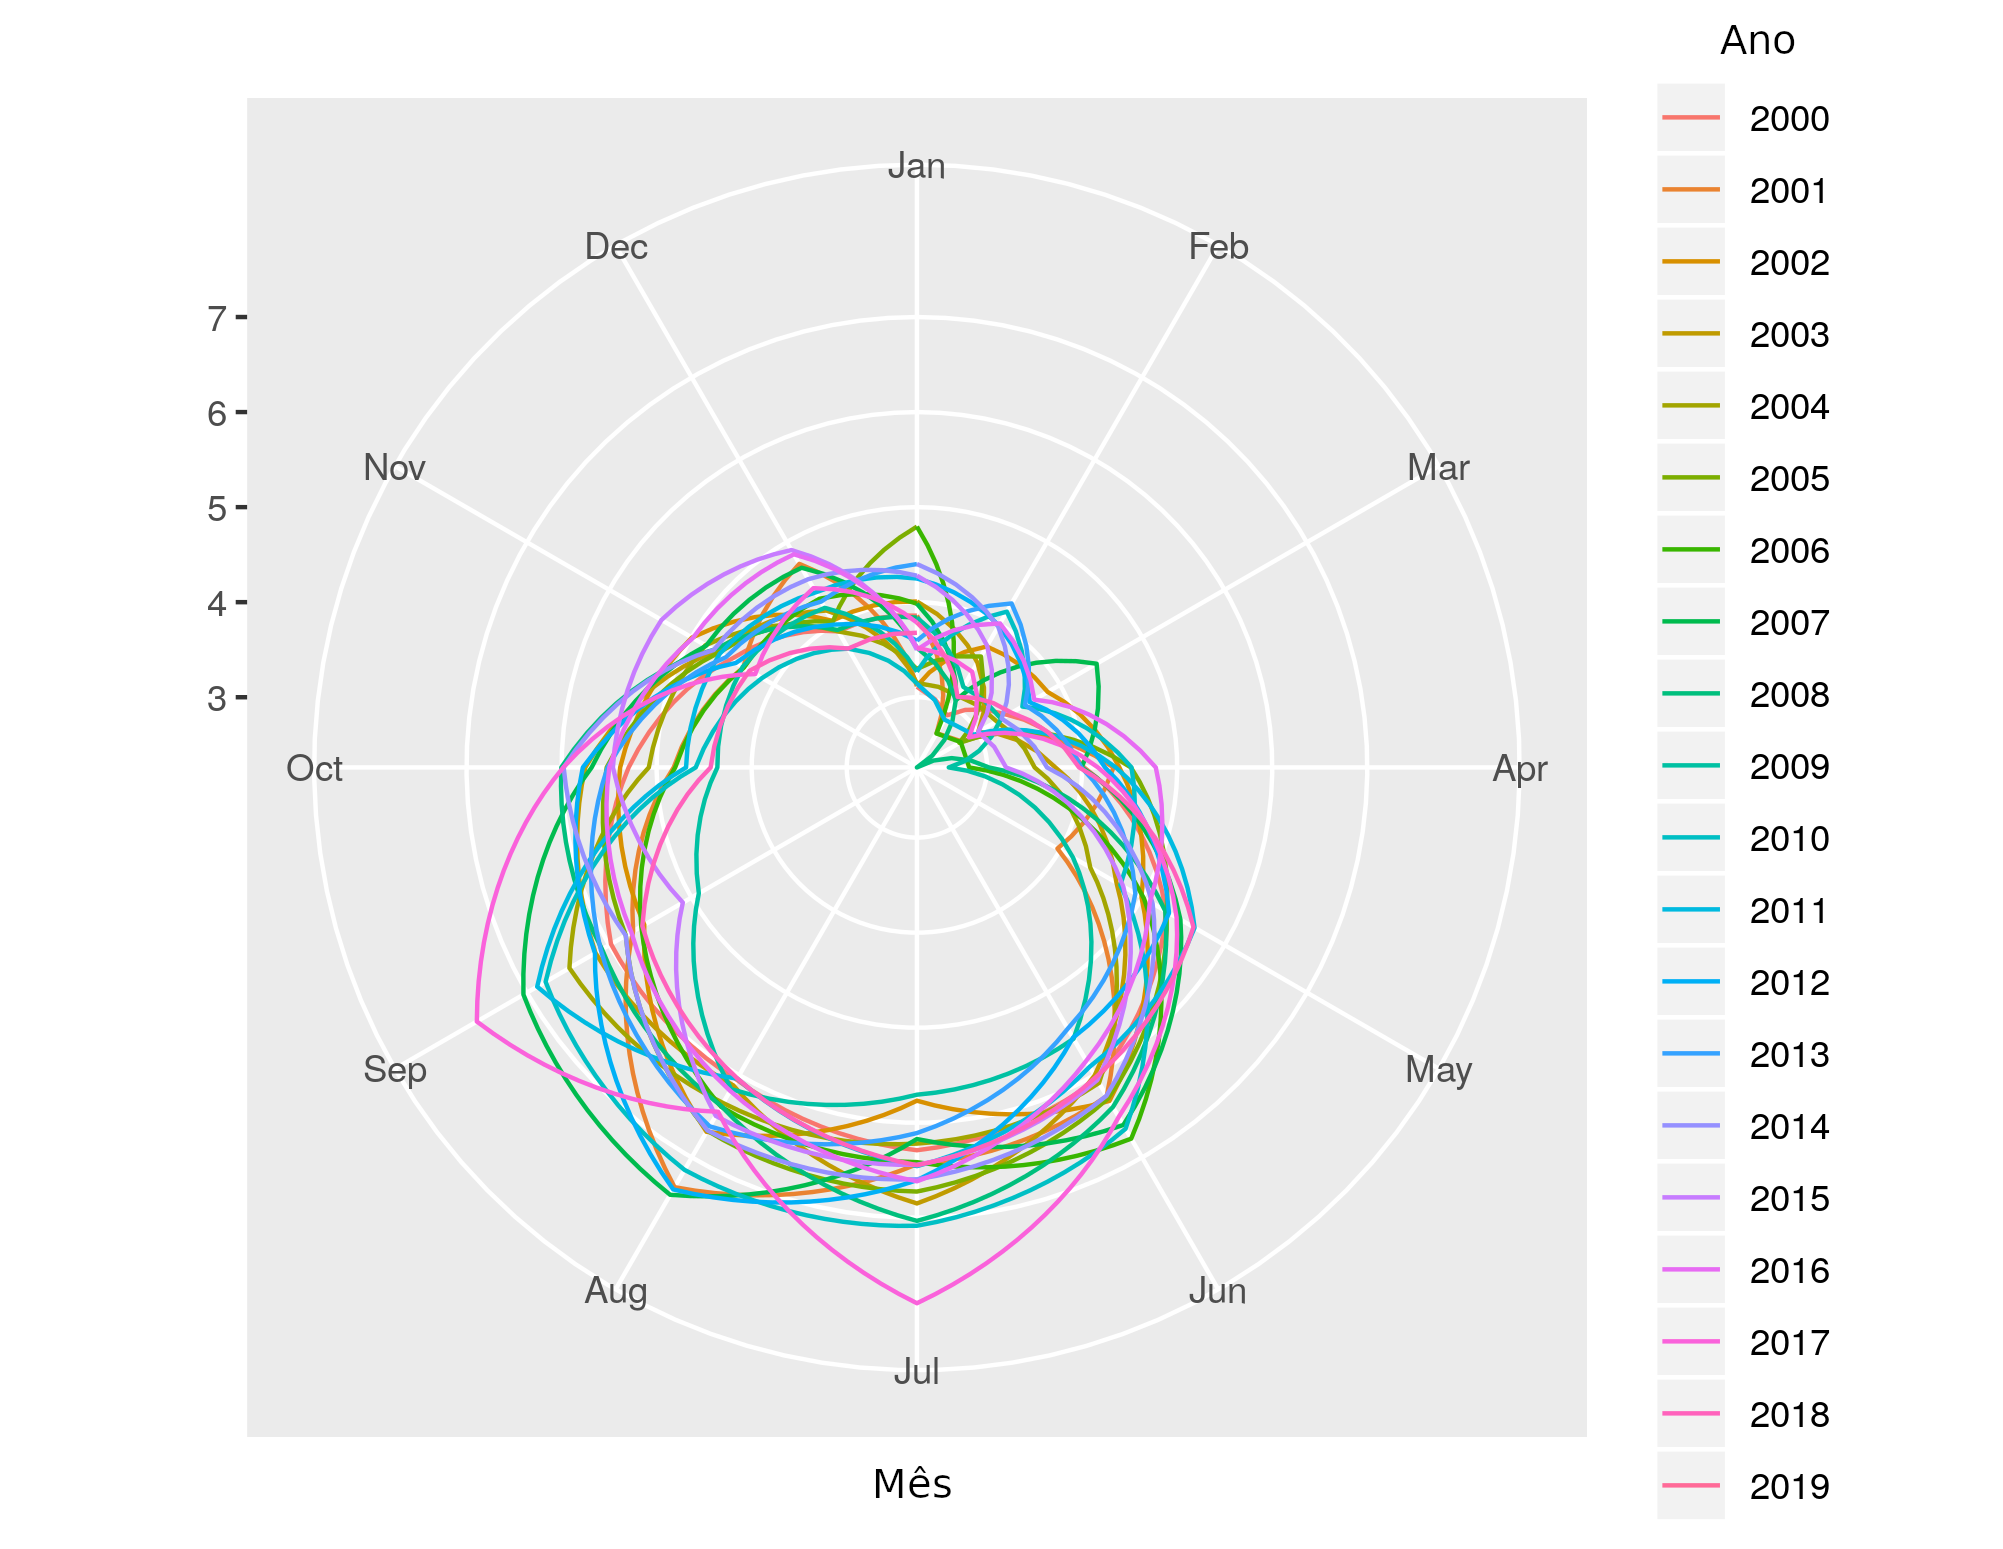
\includegraphics[width=\textwidth]{season_plot_polar}
	\caption{Velocidade média (m/s) para cada mês do ano em forma polar. Cada curva representa algum ano entre 2000 e 2019. Baseado na série de dados ERA5 da \cite{era5}.}
\end{figure}
\FloatBarrier

Já era possível ver no gráfico anterior em quais meses a velocidade era maior ou menor. No entanto, no gráfico acima isso fica mais evidente. Nos meses de inverno tem-se altas velocidades e nos meses de verão baixas velocidades. É possível observar também que o mês com maior média de velocidade varia ao longo dos anos: em anos recentes variou de Julho a Setembro enquanto que 10 anos atrás o vento era mais forte em Agosto.

%toda a série horária
%toda a série diária
%toda a série mensal
%toda a série 12x24
%rosa dos ventos
%ggseasonplot polar
\section{Horizonte de previsão}

O horizonte de previsão é variável. Ele depende do propósito para o qual a previsão será utilizada. Alguns parques eólicos no país fazem acordos mensais sobre a energia que será entregue a rede. Nesse caso é de grande utilidade uma previsão de quanta energia será produzida no mês seguinte. A previsão minutal ou horária é, nesse caso, pouco relevante.
Ao operador de subestação de distribuição de energia interessa saber quando ocorreram máximos e mínimos de produção de energia em base horária de modo que o sistema possa compensar as faltas e excessos sem perdas. Para ele a previsão em minutos ou horária é essencial. Neste trabalho, abordou-se tanto a previsão em escala horária quanto mensal.

Quanto mais próximo do último dado medido for a previsão, mais certeza se tem do seu valor. A previsão da velocidade do vento 12 meses no futuro é muito menos confiável do que a previsão para o mês seguinte. Por esse motivo, previsões são acompanhados de um intervalo de confiança. Um intervalo de confiança de 95\%, por exemplo, indica, com 95\% de confiança, o intervalo de valores que a velocidade medida poderá assumir.

%a região em azul escuro representa um intervalo de confiança de 85% enquanto a região em azul claro um intervalo de 95% de confiança de que o valor medido estará dentro desse intervalo.
% o cálculo do intervalo de confiança...
%let the data speak for itself
%innovation term representa tudo aquilo que não pode ser explicado pelos termos autoregressivos e de média móvel
%mesmo que houvesse um mecanismo que descrevesse perfeitamente o sistema sob estudo ainda assim ele não produziria previsões adequadas devido ao ruído inerente ao processo
%Box-Jenkins ARIMA

\section{Métodos}

Existem diversos métodos para previsão de séries temporais. Ao longo do desenvolvimento deste trabalho os seguintes métodos foram considerados: 
\begin{itemize}
\item Suavização exponencial: os valores passados contribuem para o valor atual com um peso que decai exponencialmente com a distância que se encontram em relação ao momento da previsão;
\item Box-Jenkins SARIMA: um modelo robusto que faz uso de valores passados (autorregressão, AR) e erros passados (média móvel, MA), inclui integração (I) para tornar a série estacionária e estabilizar variância, além disso conta com um processo iterativo para estimar parâmetros \cite{boxjay};
\item Rede neural de memória longa de curto prazo (LSTM) \cite{llstm}: esse modelo consegue determinar com precisão o peso que deve ser dado a valores muito distantes do momento da previsão;
\item Máquinas com vetor de suporte \cite{ssvm}: os dados passam por uma transformação não-linear que permite a sua categorização em um espaço de dimensão elevada e posterior transformação reversa para reportar a previsão.
\end{itemize}

O método escolhido foi o Box-Jenkins SARIMA.
Cada modelo assume uma série de hipóteses sobre o comportamento do que se deseja prever e possui um conjunto de parâmetros que precisam ser estimados para tal propósito. Para o modelo escolhido uma das hipóteses é de que os dados possuem autocorrelação, isto é, o valor atual depende dos n valores que o antecedem: se a velocidade foi alta um instante atrás é provável que ela seja alta agora, se no momento anterior o regime foi turbulento, é provável que no momento seguinte ele permaneça turbulento. Essa hipótese corresponde ao caráter autorregressivo do modelo. Outra hipótese do modelo é de que existe autocorrelação não apenas em valores passados, mas também nos erros passados. Essa hipótese corresponde ao caráter de média móvel do modelo. A interpretação dessa hipótese não é tão óbvia, mas seu uso se justifica pelo fato de que um processo AR com infinitos termos pode ser descrito por um processo MA com finitos termos e vice-versa. No contexto de séries temporais o princípio da parcimônia dita que dentre os modelos que  caracterizem uma série, se escolha aquele com menos parâmetros. Dessa forma a combinação de termos AR e MA permite que a estrutura da série seja capturada com poucos parâmetros.


\part{Implementação}

Este trabalho faz uso de um modelo linear estocástico que tem como hipótese que a série temporal sob análise é gerada por uma combinação de choques aleatórios. Essa hipótese foi inicialmente proposta por Yule e Walker \cite{yulewalker} e estendida por diversos outros autores.
Na literatura uma extensão desse modelo é conhecida como modelo autorregressivo com média móvel (ARMA, do inglês autoregressive moving-average).
O modelo descreve um processo estocástico com base nos seus valores anteriores $v_{t-k}$ e nos erros anteriores $\varepsilon_{t-k}$:

\begin{equation}
v_t = \beta_1 v_{t-1} + \dots + \beta_p v_{t-p} + \alpha_1\varepsilon_{t-1} + \dots + \dots \alpha_q\varepsilon_{t-q} 
\end{equation}

O modelo é definido pelos parâmetros $p$ e $q$ que indicam respectivamente quantos termos de autorregressão e de erro são inclusos. Um modelo ARMA(2,2) utiliza dois termos anteriores e dois erros anteriores de modo a fazer uma previsão para um período seguinte. 

Box e Jenkins popularizaram um procedimento para selecionar os parâmetros p e q que melhor descrevem uma série temporal. Uma vez definidos os parâmetros p e q pode-se estimar os parâmetros $\alpha_{1\dots q}$ e $\beta_{1\dots p}$. Os parâmetros $\beta_{1\dots p}$ são estimados pelo método dos mínimos quadrados ou alternativamente pelo  método dos momentos \cite{yulewalker}. Já os parâmetros $\alpha_{1\dots q}$ são estimados por meio de máxima verossimilhança \cite{boxjay} ou ainda por métodos não lineares tais como pelo algoritmo de Levenberg-Marquardt \cite{marq}. Neste trabalho foram utilizados o método dos mínimos quadrados e de máxima verossimilhança como implementados na biblioteca estatística \cite{Rugarch}.

\chapter{Box-Jenkins}

Em 1970 George Box e Gwilym Jenkins introduziram um método empírico para abordar a previsão de séries temporais \cite{boxjay}. O método ficou conhecido como método de Box-Jenkins. Ele consiste de uma série de etapas que podem ser resumidas no fluxograma abaixo:

\begin{figure}[h]
    \centering
	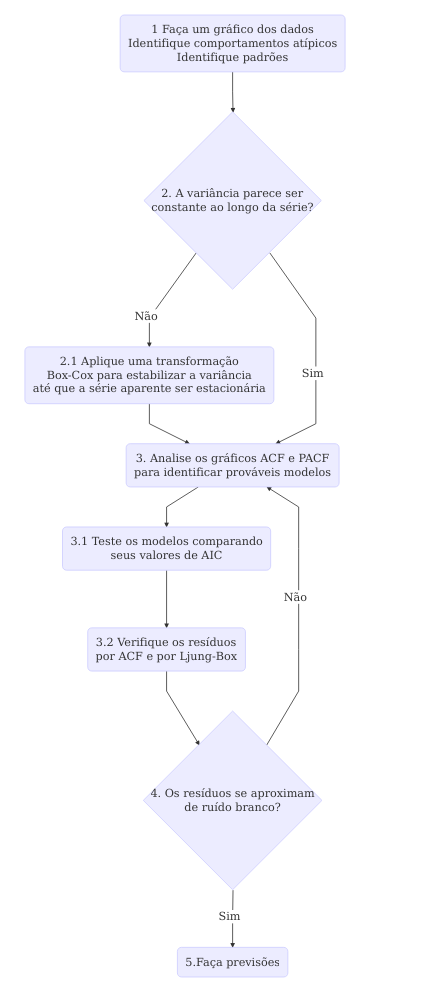
\includegraphics[scale=0.52]{boxjenkins}
	\caption{O método de Box-Jenkins.}
\end{figure}
\FloatBarrier

O fluxograma acima inclui algumas mudanças incorporadas por diversos outros autores tais como Hyndman \& Khandakar \cite{khandakar}. As métricas e testes estatísticos mencionados acima são explicadas a seguir.
O Critério de Informação de Akaike (AIC) \cite{eike} é uma métrica cuja minimização leva à melhor escolha de parâmetros p e q de modelos ARMA. O teste de Ljung-Box \cite{ljung} permite mensurar se os resíduos resultantes de um ajuste dos dados a um modelo se aproximam de ruído branco. Em caso positivo, um bom ajuste foi encontrado.

Neste trabalho, optou-se pela abordagem de Box e Jenkins para estimar séries temporais de velocidade do vento e seu uso será demonstrado a seguir.

\section{Análise visual}

A escolha do modelo para prever uma série temporal se dá pelas características dessa série, tais como: padrões, valores atípicos, tendências, sazonalidade e ciclicidade. Dessa forma, o primeiro passo é visualizar a série tanto da forma mais simples, como série temporal, quanto sob outras formas que ressaltem características que não sejam imediatamente visíveis. A transformação para o espaço de frequência, por exemplo, permite identificar se há periodicidade na série. Para facilitar a visualização, a imagem abaixo apresenta apenas os 2 últimos anos de dados em base horária:

\begin{figure}[h]
    \centering
	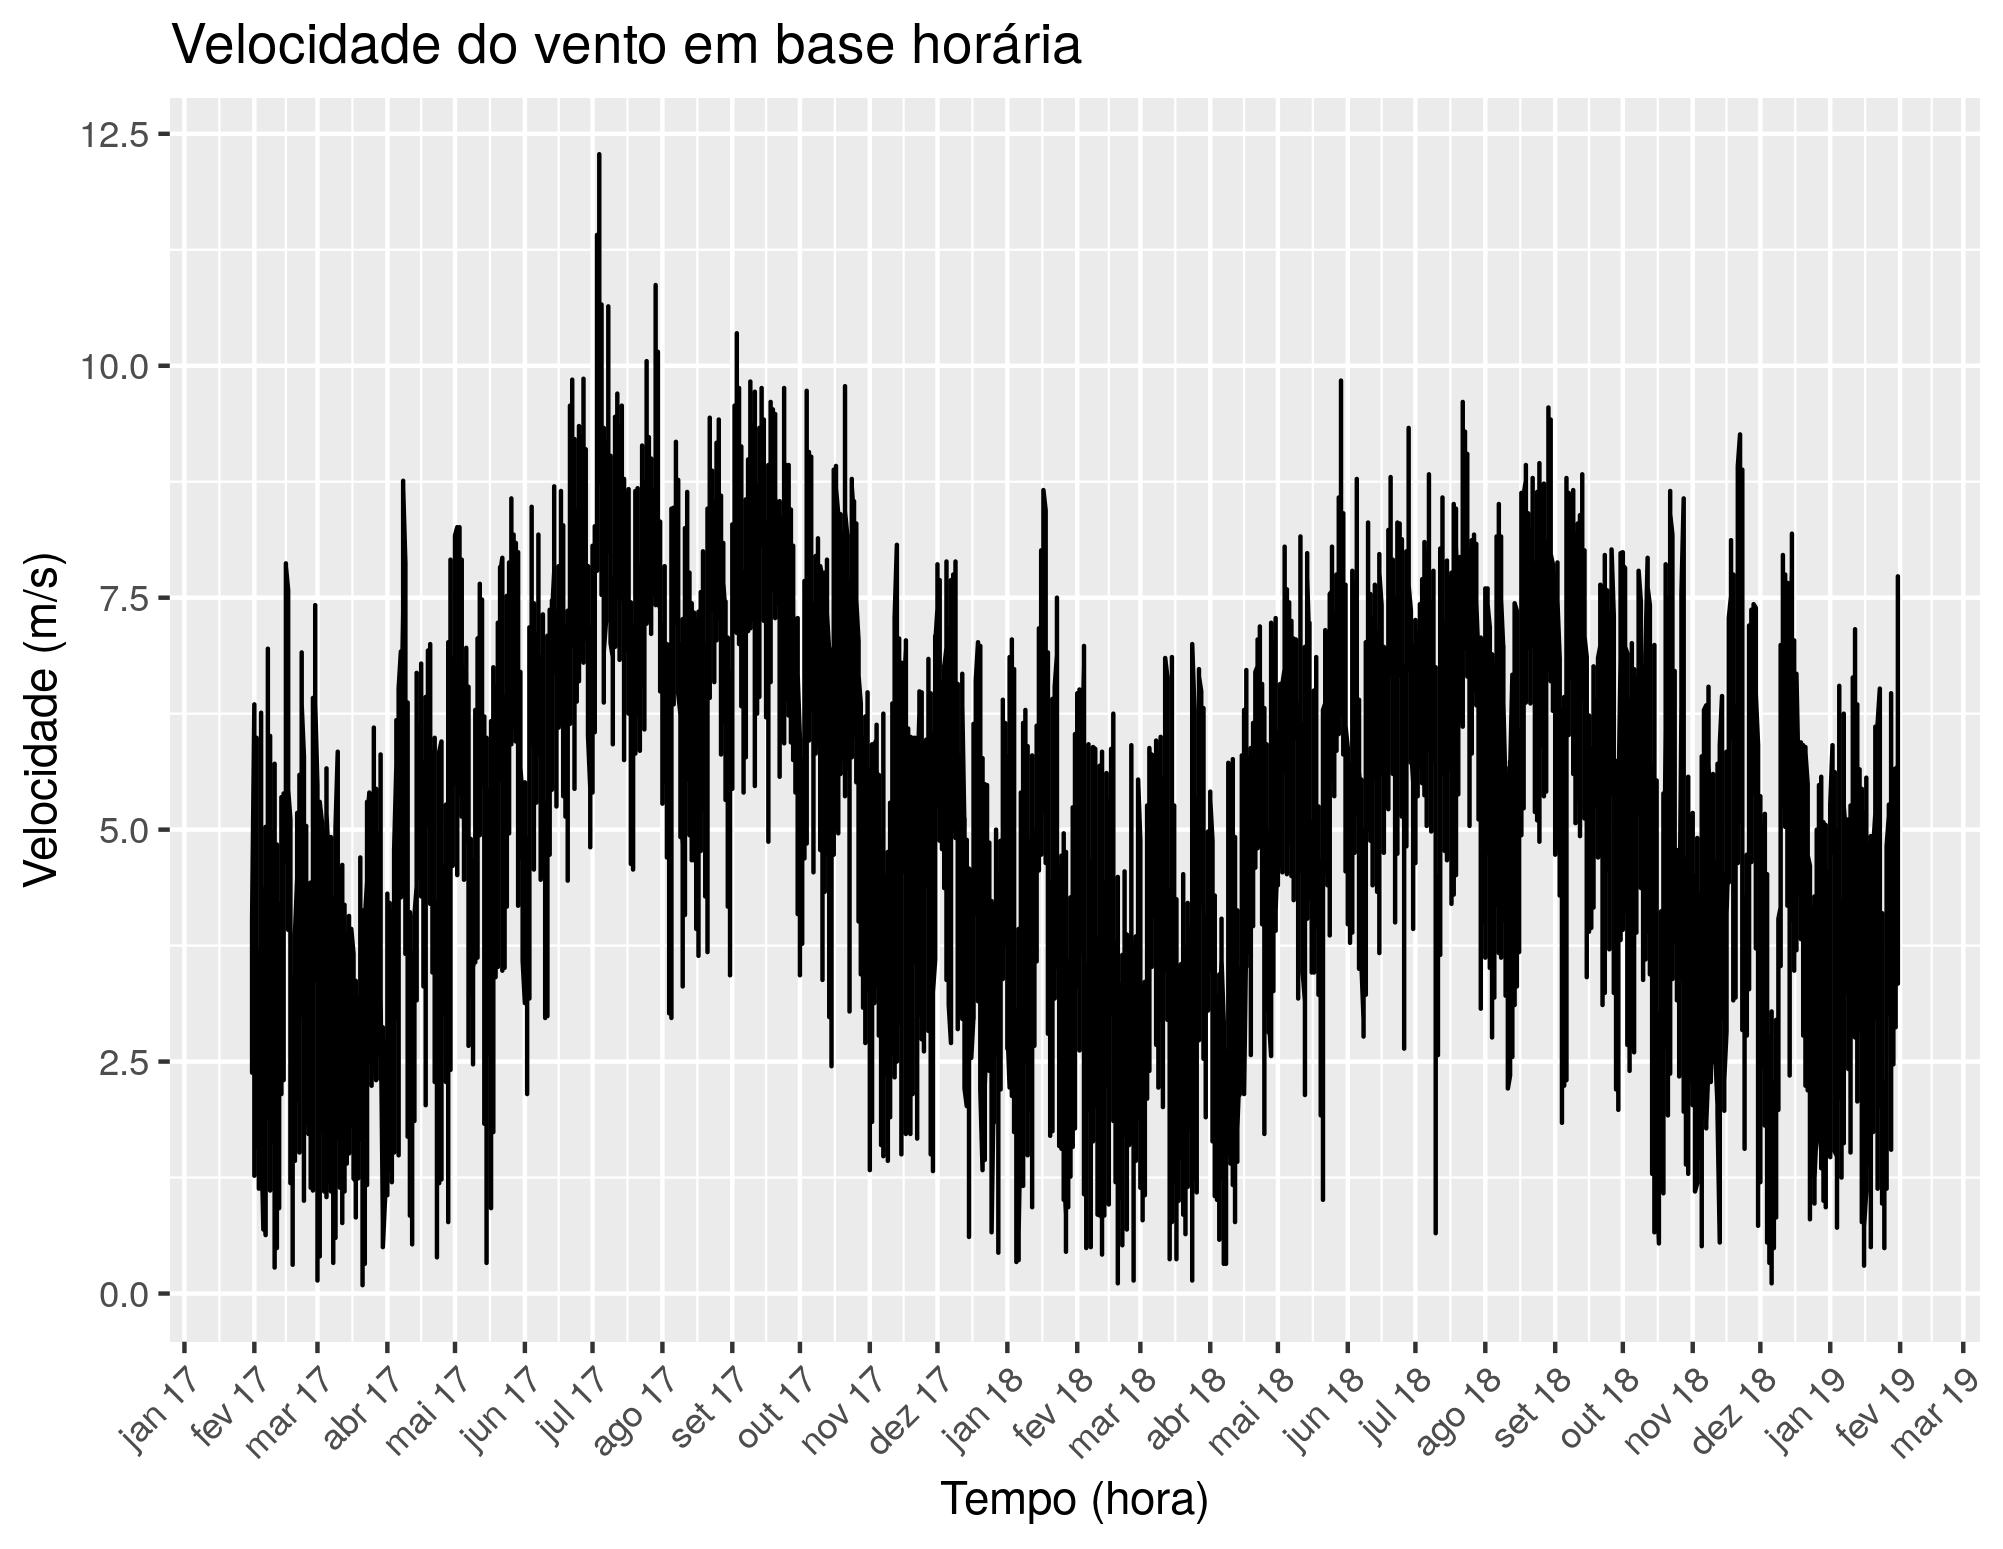
\includegraphics[width=\textwidth]{entire_series_hourly_basis}
	\caption{Últimos dois anos da série de vento. Baseado na série de dados ERA5 da \cite{era5}.}
\end{figure}
\FloatBarrier

Por meio da análise visual é possível perceber que a série não é estacionária, pois em diferentes períodos a série encontra-se em diferentes níveis (mostra uma tendência) e também apresenta sazonalidade anual.

\section{Regime estacionário}

Um processo estocástico é dito estritamente estacionário se o deslocamento da origem temporal não altera suas propriedades, ou seja, a distribuição conjunta de probabilidades calculada para a sequência de $m$ medições $z_1,z_2,\dots,z_m$ tomadas nos tempos $t_1, t_2, \dots, t_m$ é a mesma àquela calculada em $t_{1+k}, t_{2+k}, \dots, t_{m+k}$ para as m medições $z_{1+k},z_{1+k},\dots,z_{m+k}$. $k\in\mathbb{Z}$ pode assumir tanto valores positivos quanto negativos, isto é, o deslocamento temporal pode ser tanto positivo quanto negativo. Dessa forma, 
um processo estacionário é caracterizado por uma distribuição de probabilidades que não varia no tempo. O modelo autorregressivo com média móvel utilizado neste trabalho toma essa propriedade como hipótese para o seu desenvolvimento, portanto, se faz fundamental garantir que a série de entrada satisfaça tal hipótese.

O primeiro passo de modo a tornar a série estacionária é remover a sazonalidade. Isso pode ser feito por uma simples diferença entre valores consecutivos da série temporal:

\begin{figure}[h]
    \centering
	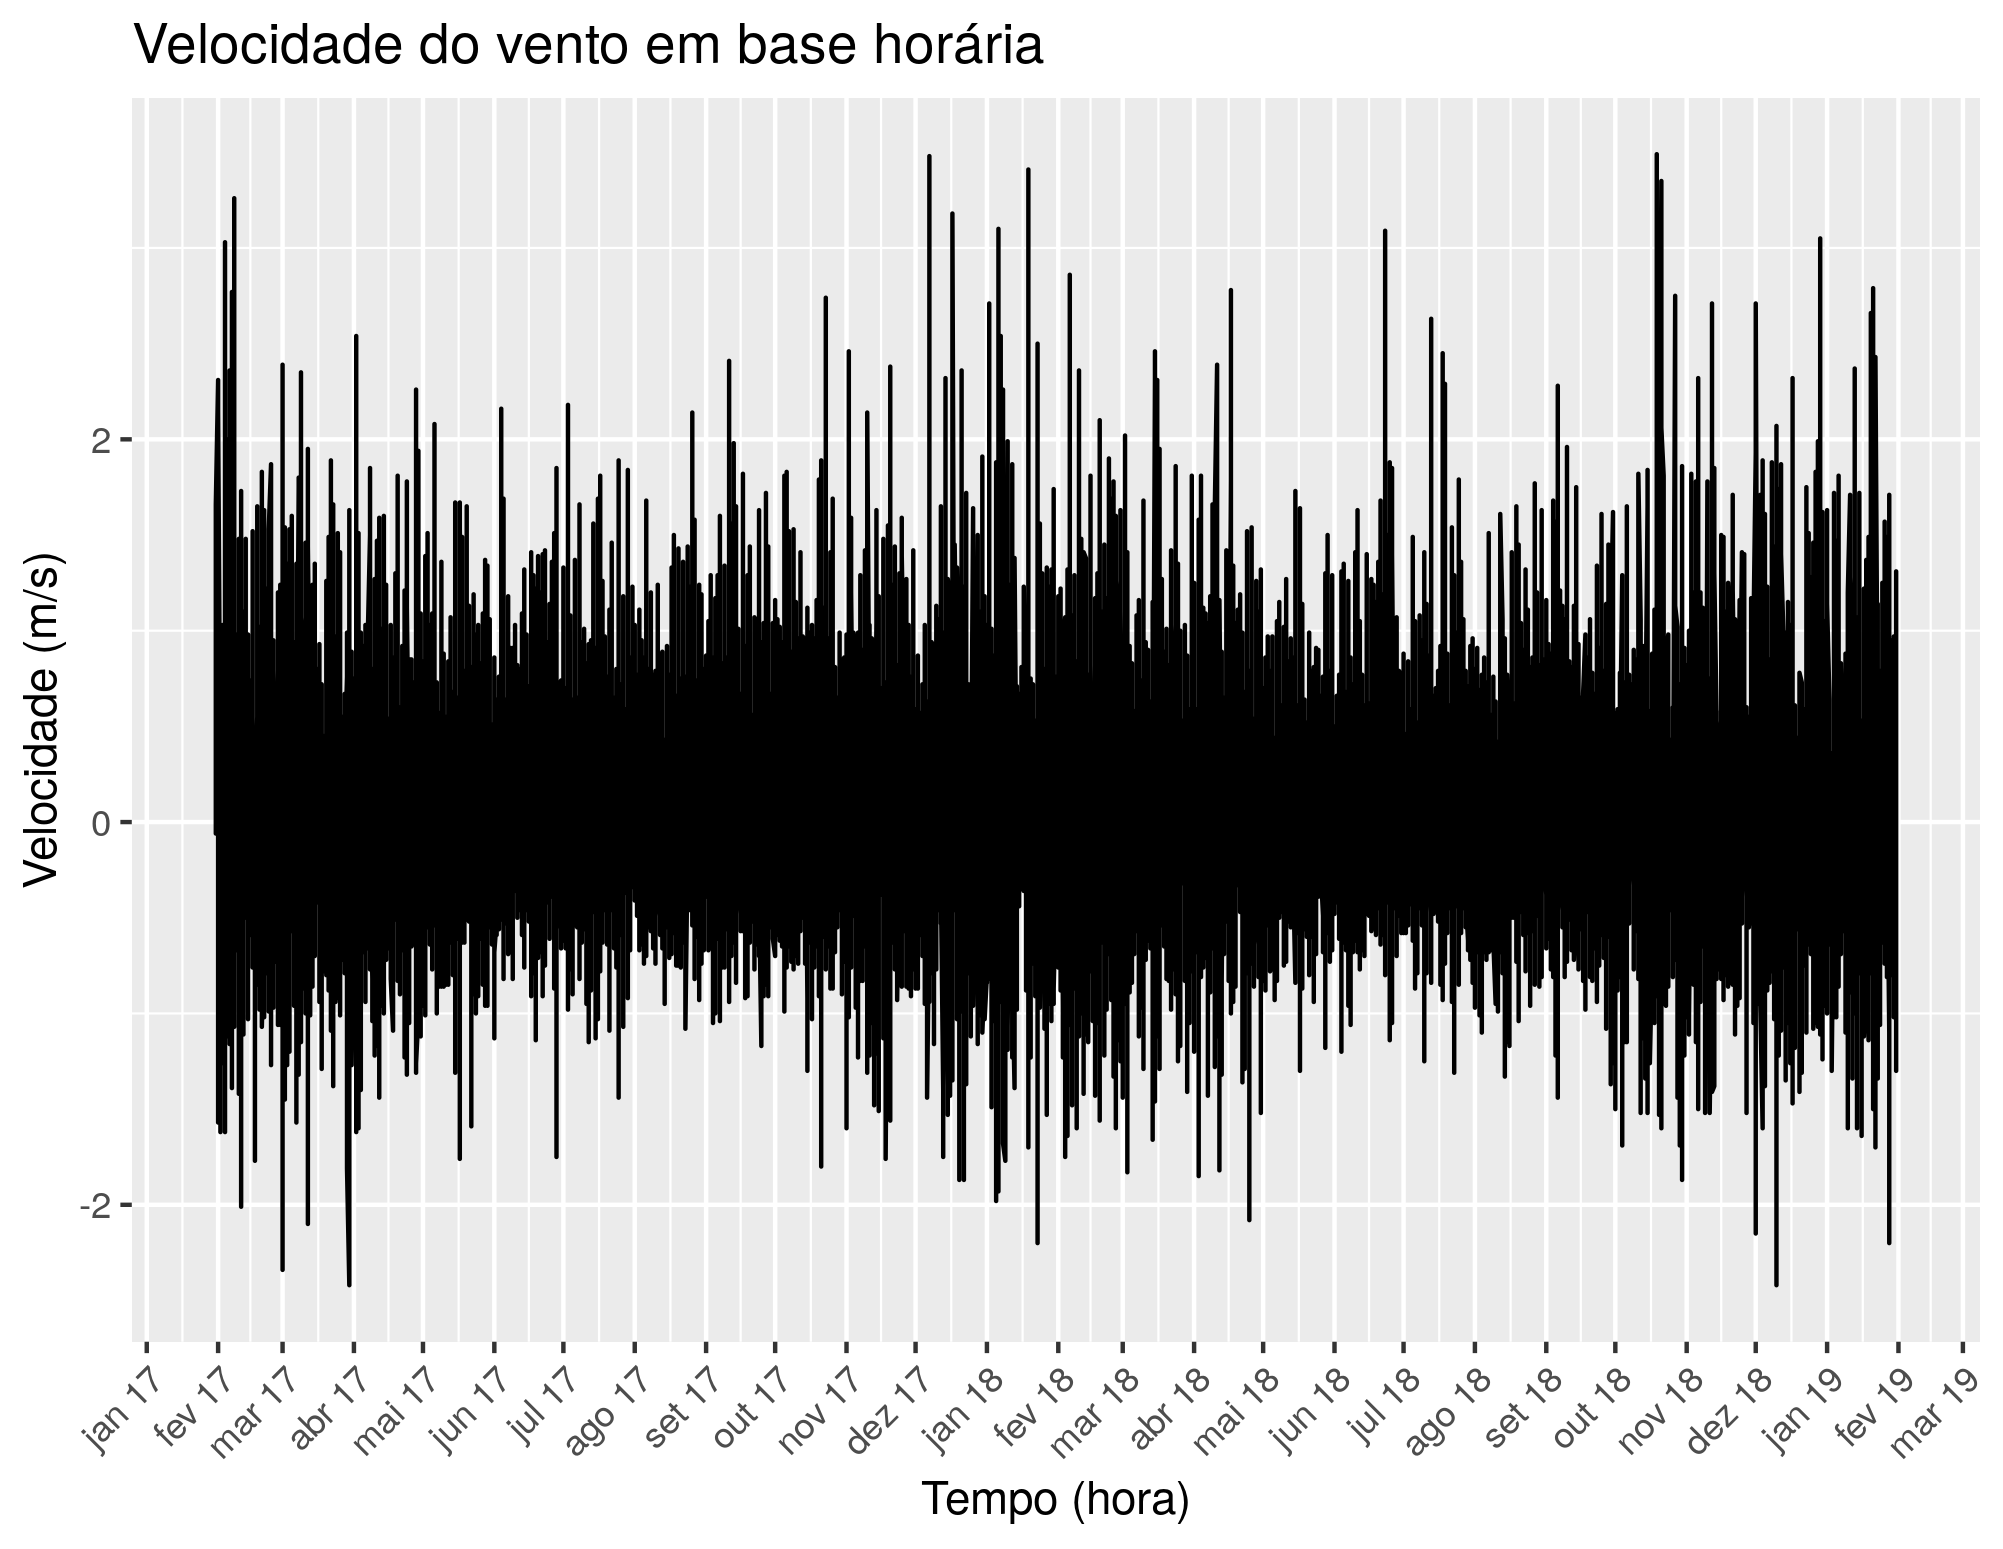
\includegraphics[width=\textwidth]{entire_series_hourly_basis_seasonless.png}
	\caption{Sazonalidade removida. Baseado na série de dados ERA5 da \cite{era5}.}
\end{figure}
\FloatBarrier

Antes de remover a sazonalidade não é possível fazer qualquer afirmação sobre o comportamento da variância. Após removê-la, por meio de uma diferenciação, percebe-se que a variância parece ter estabilizado. No entanto, essa é uma afirmação qualitativa. Pode-se obter uma confirmação quantitativa por meio de testes estatísticos chamados coletivamente como testes de raiz unitária. Optou-se por utilizar o teste Kwiatkowski-Phillips-Schmidt-Shin (KPSS) \cite{kpss} cuja hipótese nula é de que a série é estacionária (tanto em relação à tendência quanto à sazonalidade).

Aplicando o teste encontrou-se um p-valor maior que 0.1 com um nível de significância de 0.05 de tal forma que a hipótese nula não pôde ser rejeitada. Aplicando o mesmo teste antes da remoção da sazonalidade o p-valor calculado é menor que 0.01 indicando que a série não é estacionária. 

Além da simples diferença que é utilizada pare remover sazonalidade, pode-se estabilizar a variância pode meio de uma transformação de Box-Cox \cite{boxcox}. Essa transformação é definida como:

\begin{equation}
y_i^{(\lambda)} = 
	\begin{cases}
		\sqrt[n]{\prod\limits_{i=1}^{n}x_i}\ln y_i\text{, se $\lambda = 0$}
		\\
		\frac{y_i^\lambda-1}{\lambda\left(\sqrt[n]{\prod\limits_{i=1}^{n}x_i}\right)^{\lambda-1}} \text{, se $\lambda > 0$}
	\end{cases}	
\end{equation}
 
O valor de lambda calculado para a série acima foi de 1.175388. A aplicação do teste KPSS indica que a série está em regime estacionário. O resultado da transformação é exibido abaixo:

\begin{figure}[h]
    \centering
	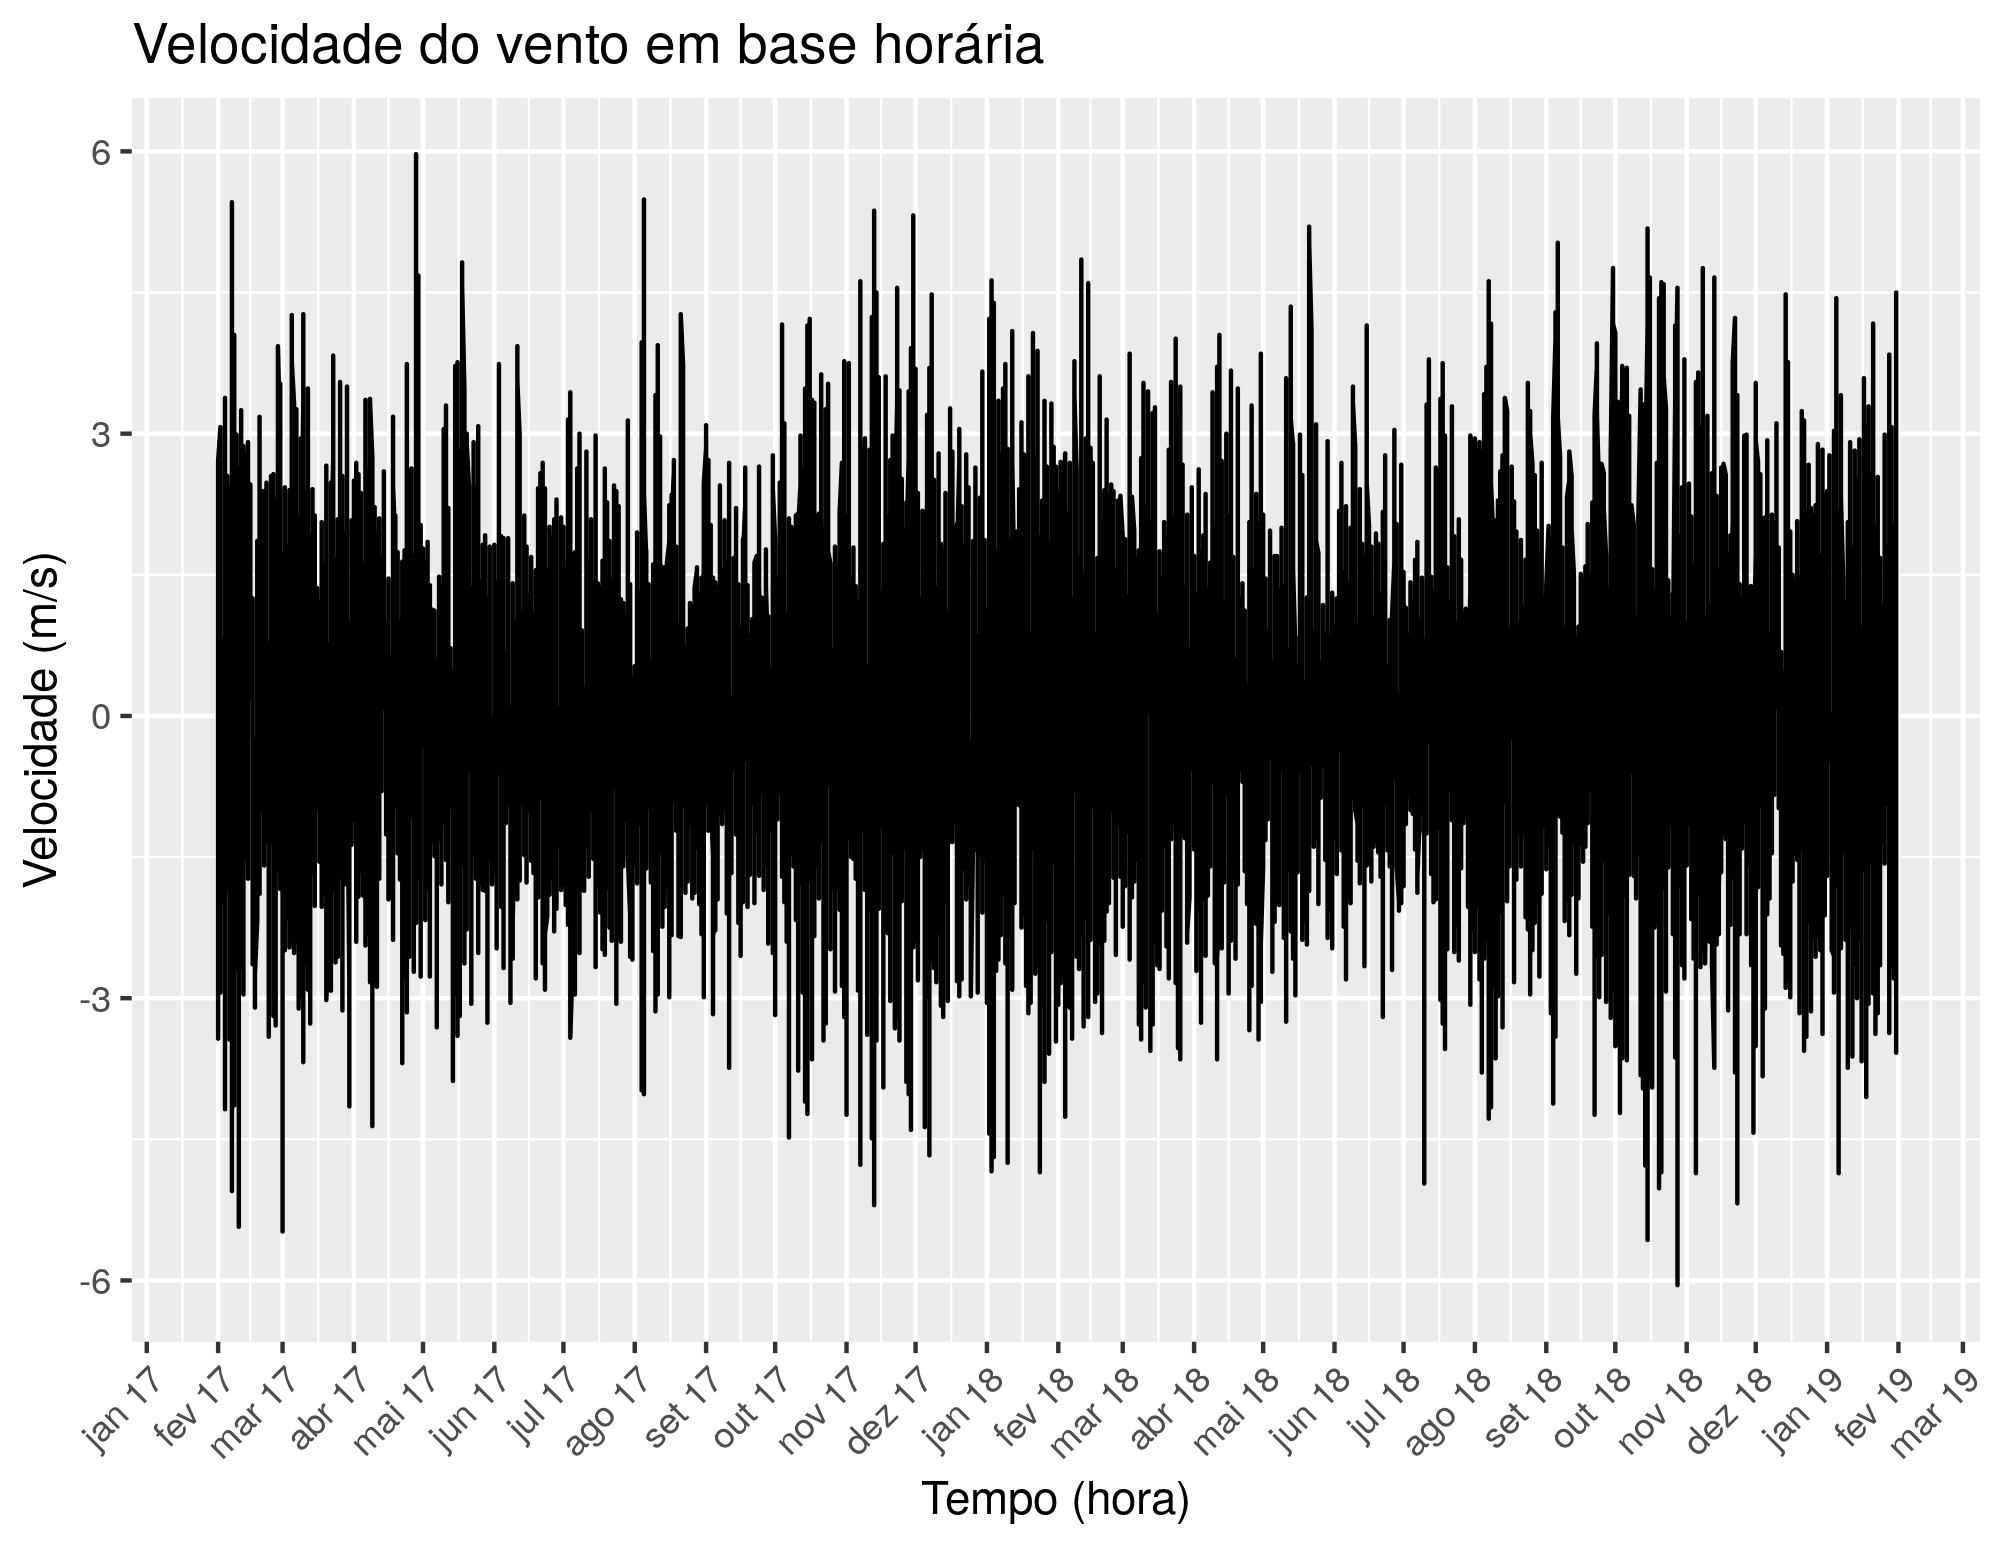
\includegraphics[width=\textwidth]{entire_series_hourly_basis_seasonless_boxcox.png}
	\caption{Variância estabilizada por meio de uma transformação de Box-Cox. Baseado na série de dados ERA5 da \cite{era5}.}
\end{figure}
\FloatBarrier 

A estabilização da variância aparenta ter sido efetiva. Como resultado deste trabalho, deseja-se obter um procedimento que possa realizar previsões para um período seguinte de maneira rápida. Essa exigência impede o uso de uma transformação Box-Cox pois devido a complexidade da operação a sua aplicação em um grande volume de dados é lenta.

Dessa forma conclui-se que o parâmetro de integração (I) do modelo ARIMA que buscamos vale $d=1$.

\section{Autocorrelação}

A etapa seguinte do método Box-Jenkins consiste em analisar os gráficos de autocorrelação e autocorrelação parcial de modo a estimar empiricamente quantos termos de autorregressão (AR) incluir e quantos de média móvel (MA).

O gráfico da função de autocorrelação (ACF) exibe o valor da correlação entre o elemento $x_i$ da série com o elemento $x_{i-k}$ para vários valores de $k$ (abcissa). O coeficiente de autocorrelação é definido por:

\begin{equation}
\rho_{t,t-k} = Corr(x_t, x_{t-k}) = \frac{Cov(x_t, x_{t-k})}{\sqrt{Var(x_t)Var(x_{t-k})}} = \frac{Cov(x_t, x_{t-k})}{\sqrt{Cov(x_t,x_t)Cov(x_{t-k},x_{t-k})}}
\end{equation}

Onde covariância (Cov) é definida por:

\begin{equation}
Cov(x,y) = E\left[(x-\mu_x)(y-\mu_y)\right]
\end{equation}

Onde $E[x]$ é o valor esperado da série temporal $x$ e $\mu_x$ seu valor médio.

Um pico na função ACF em k=12 pode significar que a série apresenta autocorrelação significativa entre um dado valor e o décimo segundo valor anterior a ele (a cada 12 horas). No entanto, isso pode ser apenas um efeito colateral de uma forte autocorrelação entre um valor e o sexto valor anterior a ele (a cada 6 horas). A função autocorrelação parcial (PACF) desconta a contribuição de todos os passos calculados anteriormente. Isso é feito mensurando a autocorrelação nos resíduos do passo $k$ após calcular a autocorrelação para o passo $k-1$. Embora o gráfico PACF seja de mais fácil interpretação, o gráfico ACF ainda é útil porque a autocorrelação não é necessariamente linear e não pode, portanto, ser simplesmente subtraída.

Os gráficos das funções ACF e PACF são exibidos abaixo. Os termos que exibem autocorrelação significativa encontram-se acima da linha azul.

\begin{figure}[h]
    \centering
	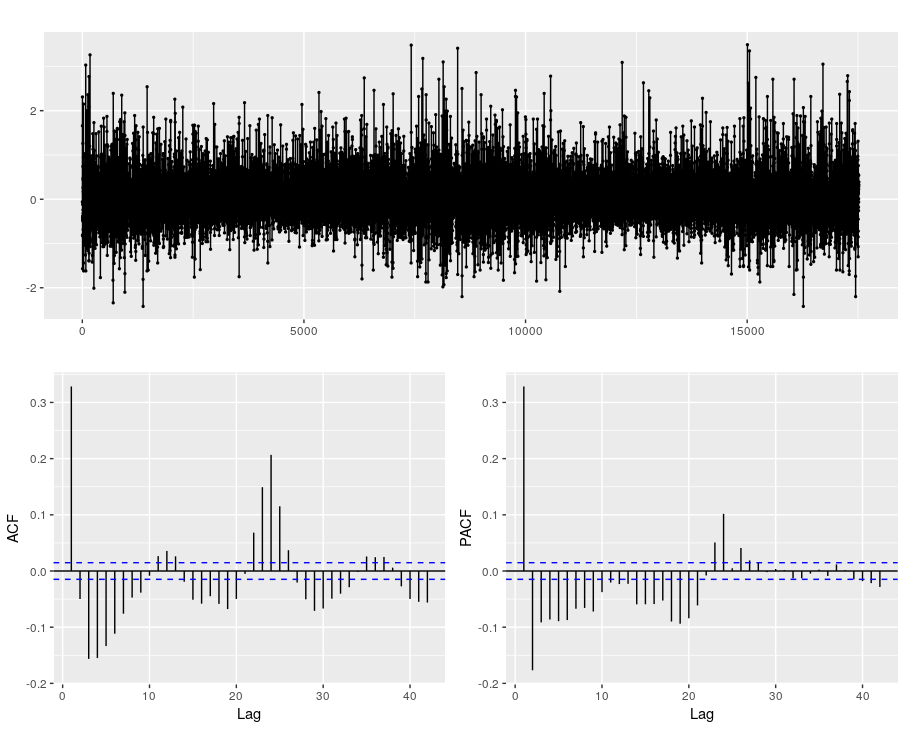
\includegraphics[width=\textwidth]{long_memory.png}
	\caption{Gráficos da Função de Autocorrelação (ACF) e Função de Autocorrelação Parcial (PACF). Baseado na série de dados ERA5 da \cite{era5}.}
\end{figure}
\FloatBarrier 

\section{Redes neurais recorrentes}

Os gráficos ACF e PACF da sessão anterior indicam que a série possui memória de longo-prazo. A série exibe autocorrelação acima do nível de significância para valores da série muito distantes entre si. Observando poucos termos anteriores pode-se crer que a autocorrelação é atenuada ao longo do tempo, no entanto, quando se considera valores mais distantes, percebe-se que a atenuação é muita lenta para permitir um modelo ARIMA.

\begin{figure}[h]
    \centering
	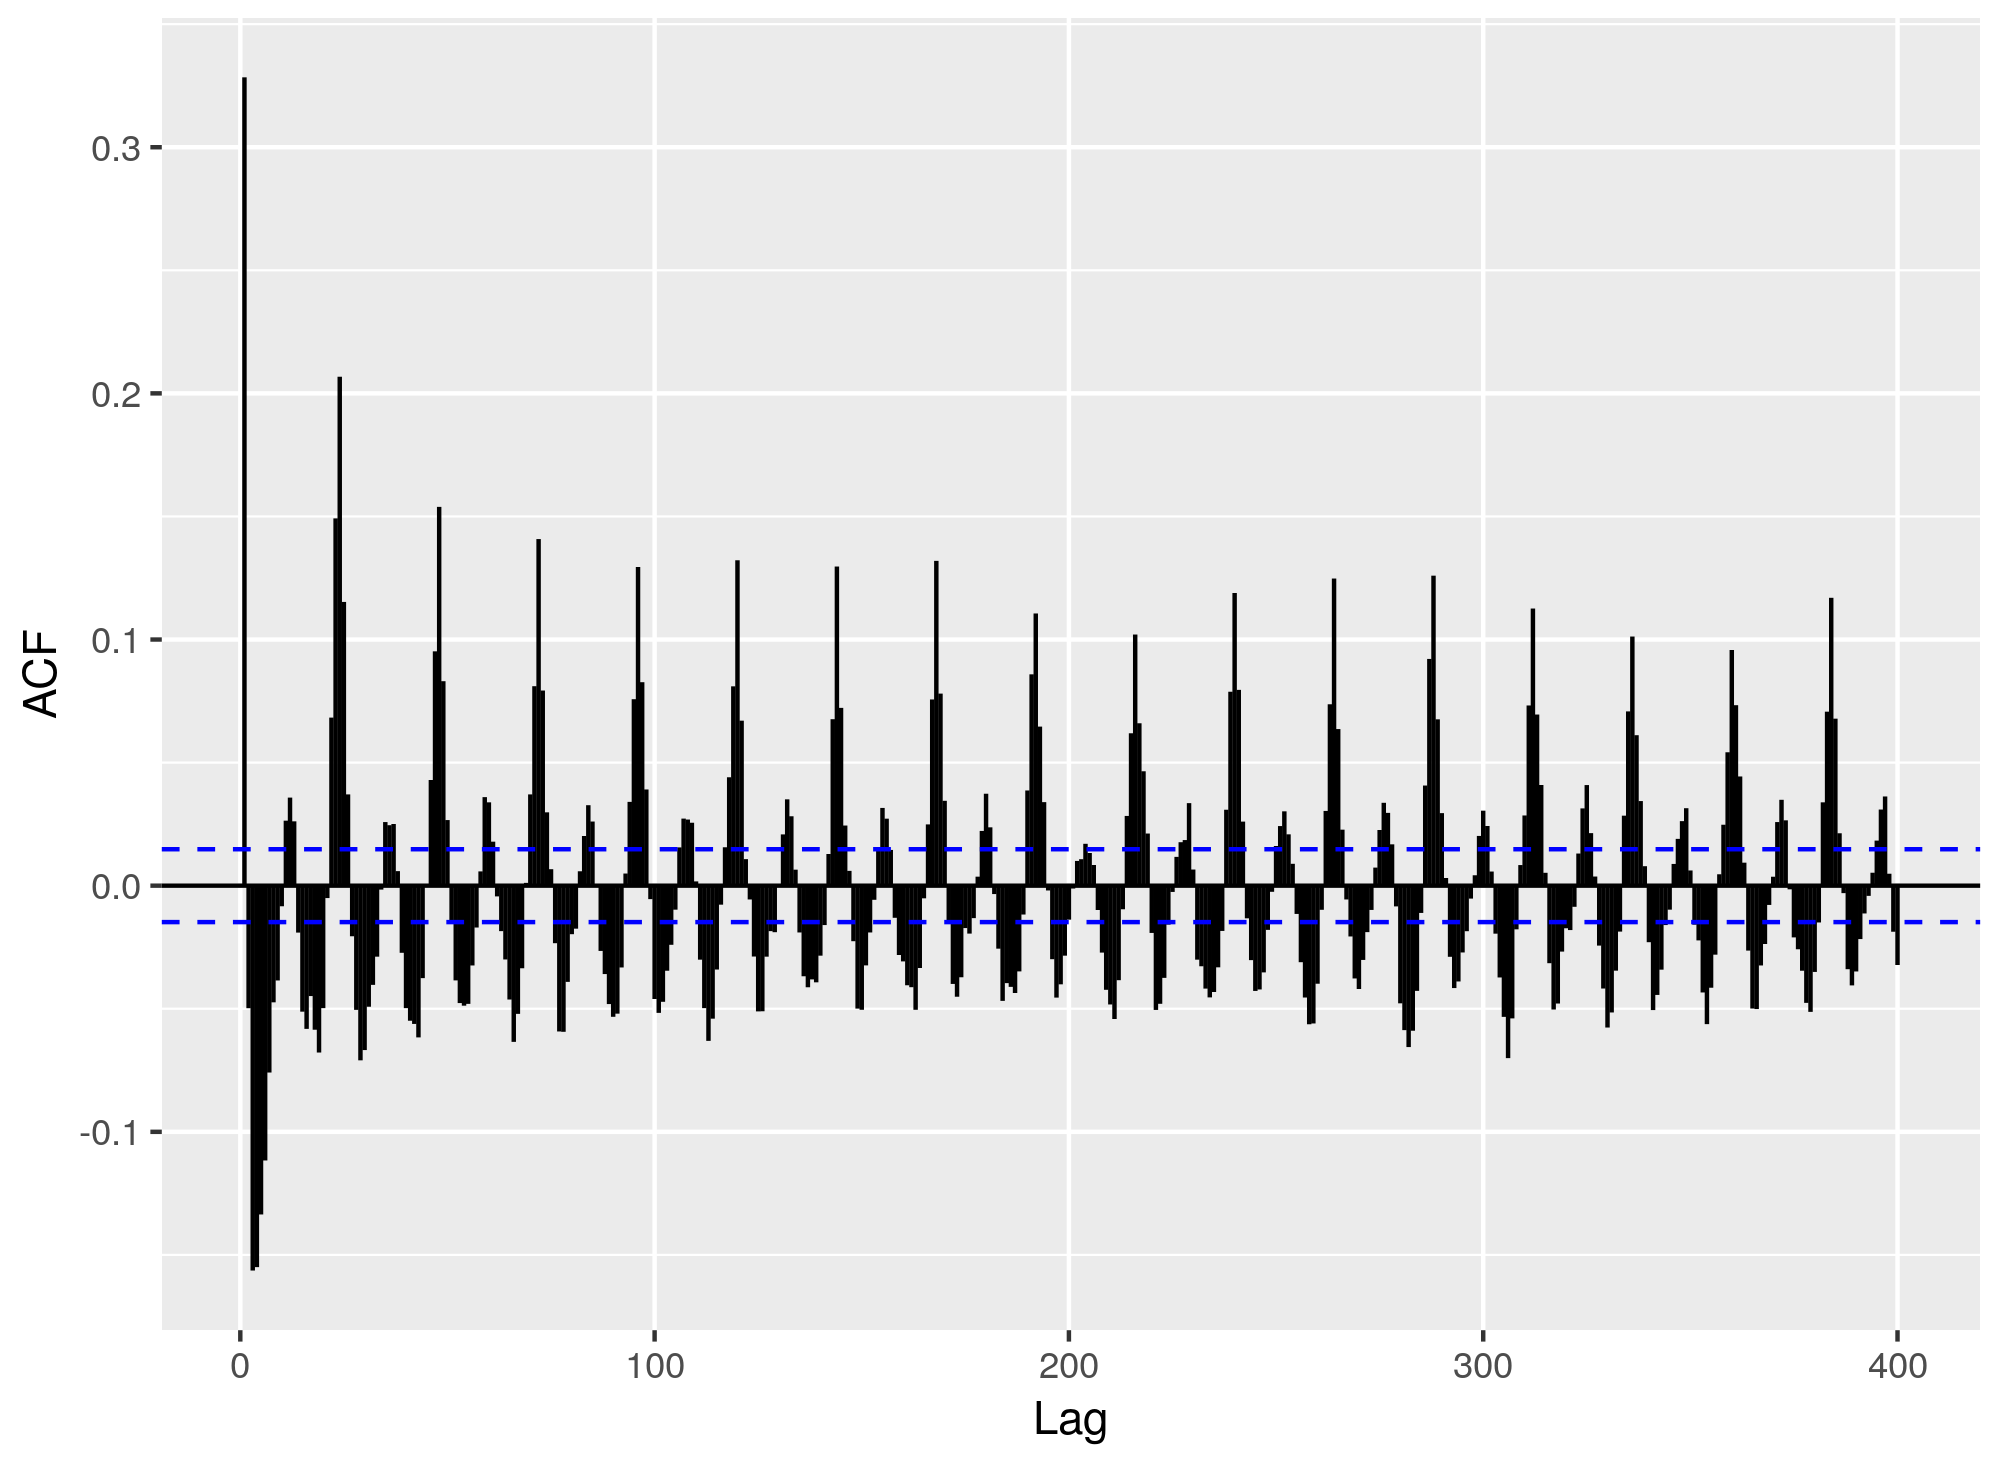
\includegraphics[width=\textwidth]{long_memory_lagmax.png}
	\caption{Gráfico da Função de Autocorrelação (ACF) evidenciando lenta atenuação de autocorrelação. Baseado na série de dados ERA5 da \cite{era5}.}
\end{figure}
\FloatBarrier 

Não é possível prosseguir naturalmente com o método de Box-Jenkins cujo próximo passo seria o teste de valores de $p$, $q$ estimados a partir dos gráficos acima. Por exemplo, caso apenas a primeira e segunda componente do gráfico PACF fosse significativa, testar-se-ia um modelo ARIMA(2,1,0).

É necessário uma mudança de abordagem. Duas tentativas foram feitas. A primeira consistiu em abandonar modelos ARIMA e optar por uma modelo de rede neural recorrente. O modelo supostamente mais adequado é o modelo de Memória Longa de Curto Prazo (LSTM) o qual consegue levar em conta a existência de memória de longo prazo na série e utilizar na previsão de curto prazo. Experimentou-se com vários modelos utilizando-se as bibliotecas Keras \cite{keras} e TensorFlow \cite{tensorflow}. O modelo resultante contou com 1 camada de entrada, 1 camada oculta com 4 blocos LSTM com uma camada de saída, todas intercaladas com uma camada de descarte para evitar aprendizado em excesso (ajuste exacerbado). Apesar do esforço empregado, não foi possível encontrar parâmetros adequados para o modelo. O resultado da previsão, mostrado abaixo, foi insatisfatório. Acredita-se que um maior esforço no entendimento e adequada configuração pudesse trazer melhores resultados, no entanto, optou-se por abandonar esse modelo devido ao longo tempo de treinamento, isto é, o tempo em que o código leva para olhar para os valores passados da série e estimar os parâmetros utilizado na previsão de valores futuros.

\begin{figure}[h]
    \centering
	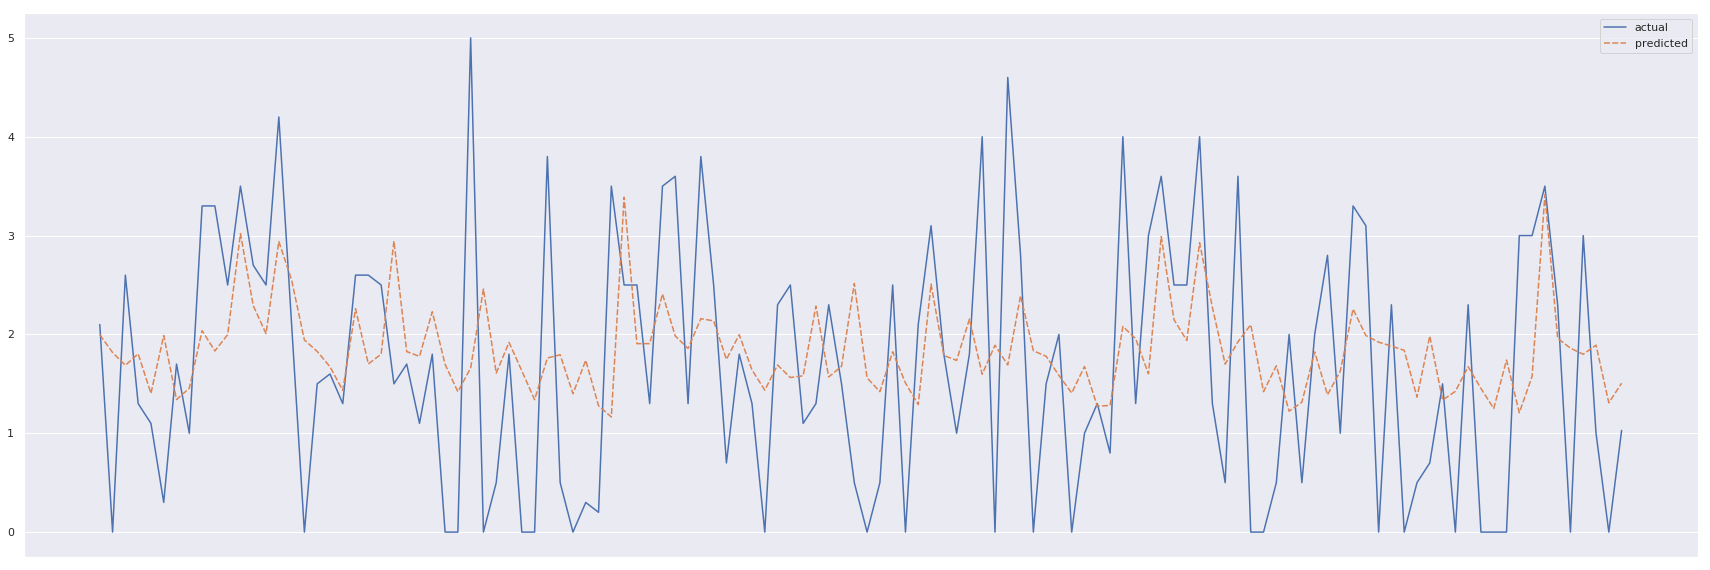
\includegraphics[width=\textwidth]{lstm.png}
	\caption{Modelo LSTM aplicado a série. Velocidade (m/s) na ordenada. Tempo (h) na abscissa. Baseado na série de dados ERA5 \cite{era5}.}
\end{figure}
\FloatBarrier 

\section{Janela de dados}\label{janela}

A segunda abordagem para contornar o problema de memória longa da série consiste em restringir a janela de dados. Por um lado, a restrição do intervalo de análise da série resolve o problema de memória de longo-prazo (não há mais longo-prazo). Por outro lado, os parâmetros estimados para um janela de dados pode não ser válido para a janela seguinte, exigindo, dessa forma, o cálculo constante dos novos parâmetros a medida que a janela cobre toda a série. Desde que o tempo para o cálculo desses parâmetros seja menor que o tempo de aquisição dos dados, a exigência é apenas a de ter hardware dedicado a esse cálculo ininterruptamente. Essa abordagem também permite que mudanças na série sejam facilmente incorporadas ao modelo, tal como, por exemplo, trocar a série horária por uma série de 10 minutos ou uma mudança natural de tendência na série devido, por exemplo, ao aumento ou diminuição da temperatura da região.

Dessa forma, decidiu-se por restringir a janela de dados a semanas ao invés de anos. A última semana de dados é exibida abaixo. Aplicando o teste KPSS percebe-se que é necessária uma diferenciação na série para torná-la estacionária.

\begin{figure}[h]
    \centering
	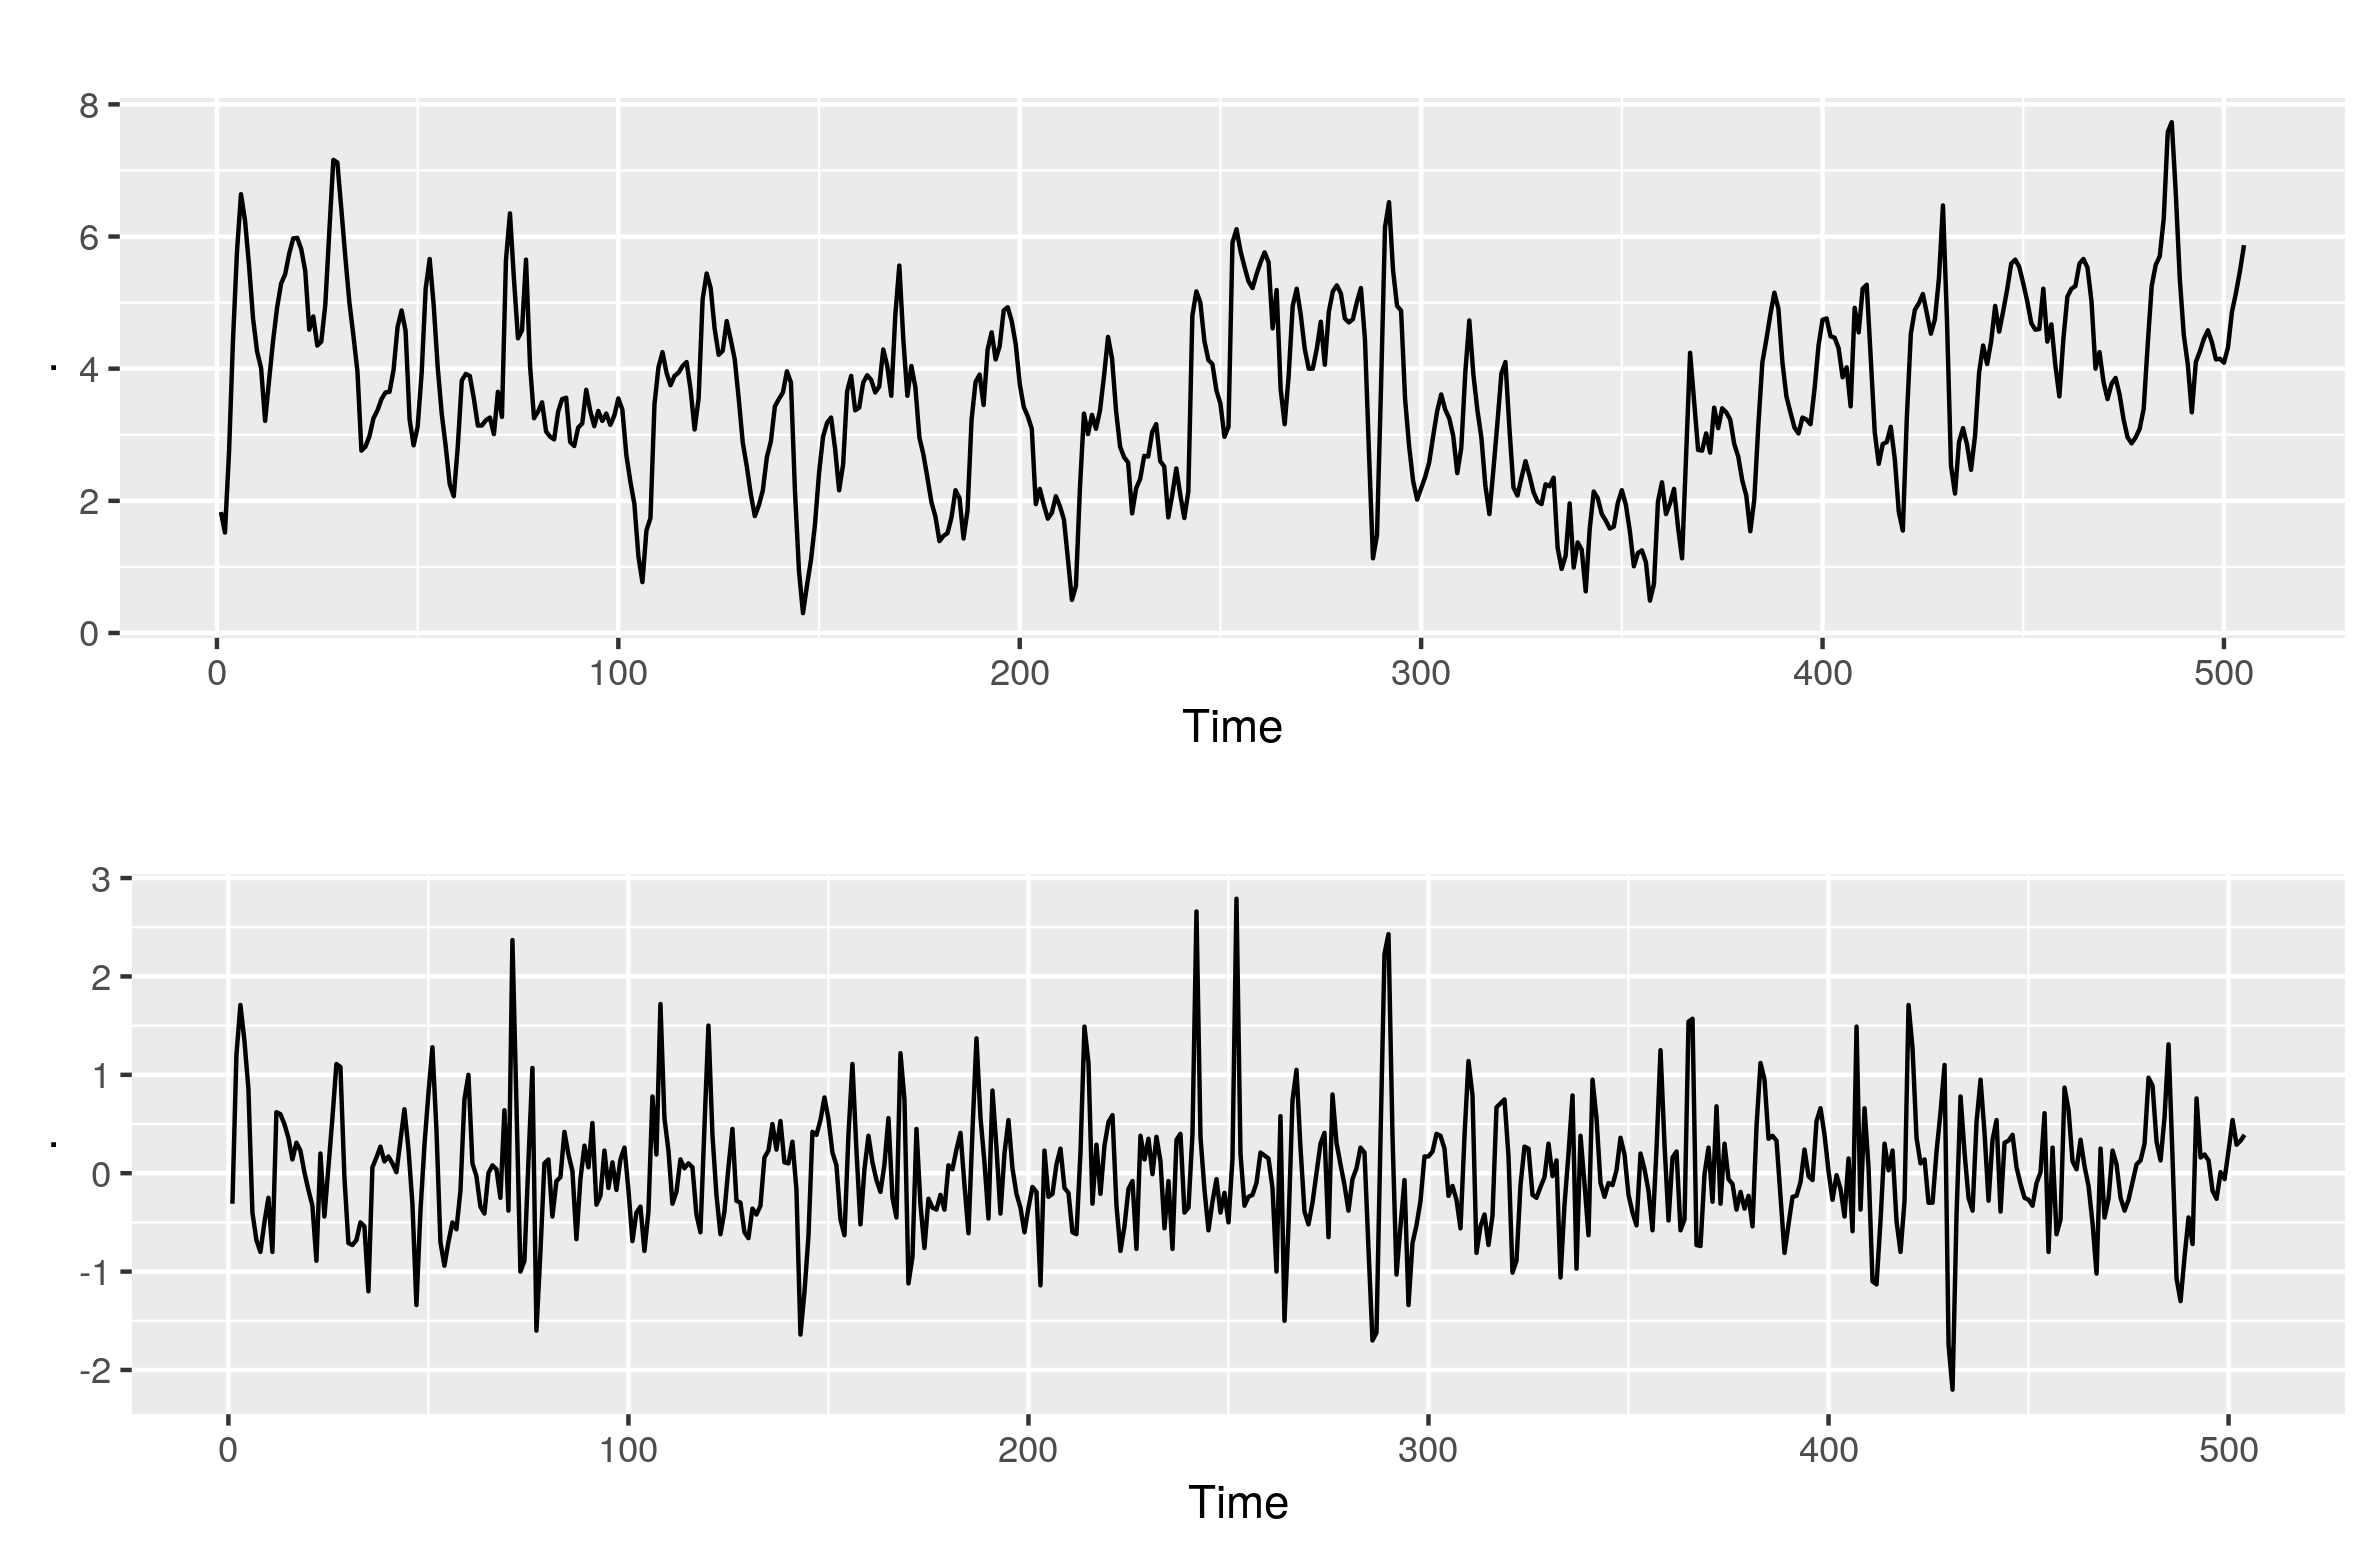
\includegraphics[width=\textwidth]{last3weeks.png}
	\caption{3 últimas semanas de dados da série. Antes da diferenciação (superior) e após (inferior). Baseado na série de dados ERA5 \cite{era5}.}
\end{figure}
\FloatBarrier 

Analisando os gráficos das funções de autocorrelação é possível elencar alguns possíveis modelos ARIMA. O gráfico da função ACF indica quantos termos MA incluir enquanto a função PACF indica quantos termos AR incluir. De acordo com a ACF a influência de autocorrelação se estende apenas até o sexto termo. No entanto, o valor respectivo está próximo do nível de significância e não é tão simples satisfazer as condições de convergência quando se inclui muitos termos MA, portanto, é interessante testar um modelo MA(3). A função PACF apresenta um valor significativo para o termo imediatamente anterior sugerindo um modelo AR(1). 

\begin{figure}[h]
    \centering
	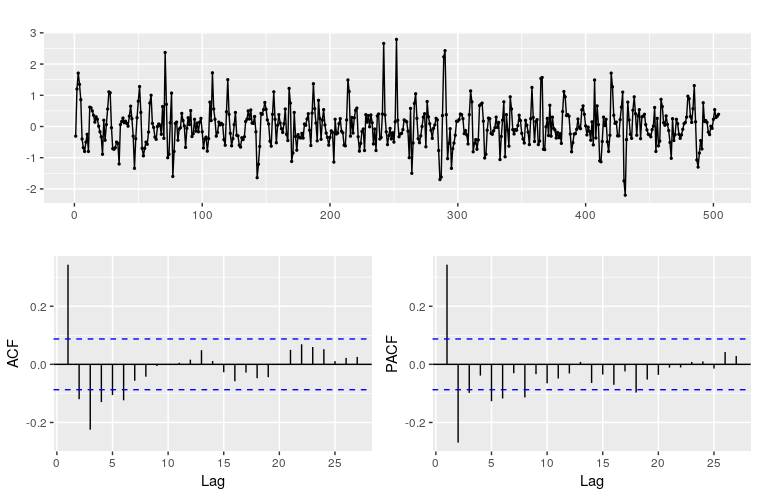
\includegraphics[width=\textwidth]{last3weeks_acf.png}
	\caption{Gráficos da Função de Autocorrelação e Autocorrelação Parcial para 2 semanas de dados da série. Baseado na série de dados ERA5 \cite{era5}.}
\end{figure}
\FloatBarrier 

Após essas observações empíricas, pode-se testar quantitativamente o desempenho de alguns possíveis modelos:

\begin{itemize}
	\item ARIMA(0,1,1)
	\item ARIMA(1,1,1)
	\item ARIMA(1,1,2)
	\item ARIMA(1,1,3)
\end{itemize}

Antes de fazer previsões é necessário estabelecer critérios para comparar o desempenho de diferentes modelos.

\section{Medidas de qualidade de previsões}\label{erro}

Para prever e quantificar a qualidade da previsão de uma série temporal é necessário dividi-la em um conjunto de treinamento e outro de teste. A divisão pode ser, por exemplo, 80\% dos dados destinados ao conjunto de treinamento e os 20\% subsequentes ao conjunto de teste. Empiricamente, é desejável que o conjunto de teste seja maior ou igual do que o horizonte de previsão que se deseja obter. O conjunto de treinamento é utilizado para computar os parâmetros do modelo, enquanto que o conjunto de teste é utilizado para quantificar o quão bem o modelo é capaz de prever os dados subsequentes.
Existem diversas maneiras de mensurar a qualidade das previsões geradas por um modelo. Deve-se evitar usar os resíduos como medida pois eles são resultado da estimativa dos parâmetros do modelo aos dados de treinamento. Como qualquer série pode ser aproximada por um modelo com infinitos parâmetros, os resíduos não dão informação sobre o poder preditivo do modelo para valores futuros, desconhecidos. 
% previsão de séries temporais sempre envolve um equilíbrio entre overfitting: aproximar uma série com muitas parâmetros, sendo capaz de prever apenas valores dentro do conjunto de treinamento; e underfitting: não capturar a estrutura da série

O erro de previsão é dado pela diferença entre o valor medido, $y_{t+h}$, e o valor previsto pelo modelo, $\hat{y}_{t+h}$:

$$e_{t+h} = y_{t+h} - \hat{y}_{t+h}$$

Existem muitas maneiras de quantificar o erro de previsão. As características de algumas delas são abordadas nas seções seguintes com o propósito de definir o modo pelo qual os resultados de previsão serão quantificados nesse trabalho.

\subsection{Erro médio absoluto (MAE)}

O erro absoluto médio é dado pela média do módulo do erro de previsão. Essa medida penaliza o resultado tanto por erros negativos quanto positivos. A minimização dessa medida de erro resulta em estimativas que se aproximam da mediana dos dados.

$$\text{MAE} = \frac{1}{T}\sum_{t=1}^{T}\left|e_{t}\right|$$

\subsection{Raíz do quadrado da média do erro (RMSE)}

A raíz do quadrado da média do erro é dada por:

$$\text{RMSE} = \sqrt{\frac{1}{T}\sum_{t=1}^{T}e_{t}^2}$$

A minimização dessa medida de erro resulta em estimativas que se aproximam da média dos dados.

\subsection{Erro absoluto médio escalonado (MASE)}

Ao contrário das medidas anteriores, essa possui a vantagem de que é independente da escala dos dados medidos:

$$\text{MAPE} = \frac{\frac{1}{T}\sum_{t=1}^T\left|e_t\right|}{\frac{1}{T-1}\sum_{t=2}^{T}\left|y_t-y_{t-1}\right|}$$

\subsection{Validação cruzada}\label{cruzada}

A validação cruzada consiste em usar uma janela de treinamento para calcular o erro de previsão para a próxima medida, expandir a janela em uma medida e calcular o novo erro e assim por diante sob um conjunto de teste. A medida de erro é dada pela média dos erros individuais. Qualquer uma das medidas acima pode ser utilizada no cálculo da validação cruzada. Essa é a maneira mais robusta de quantificar o erro de previsão já que atua efetivamente em dados que não foram utilizados para construir o modelo. A ideia da medida pode ser ilustrada da seguinte forma:

\begin{figure}[h]
    \centering
	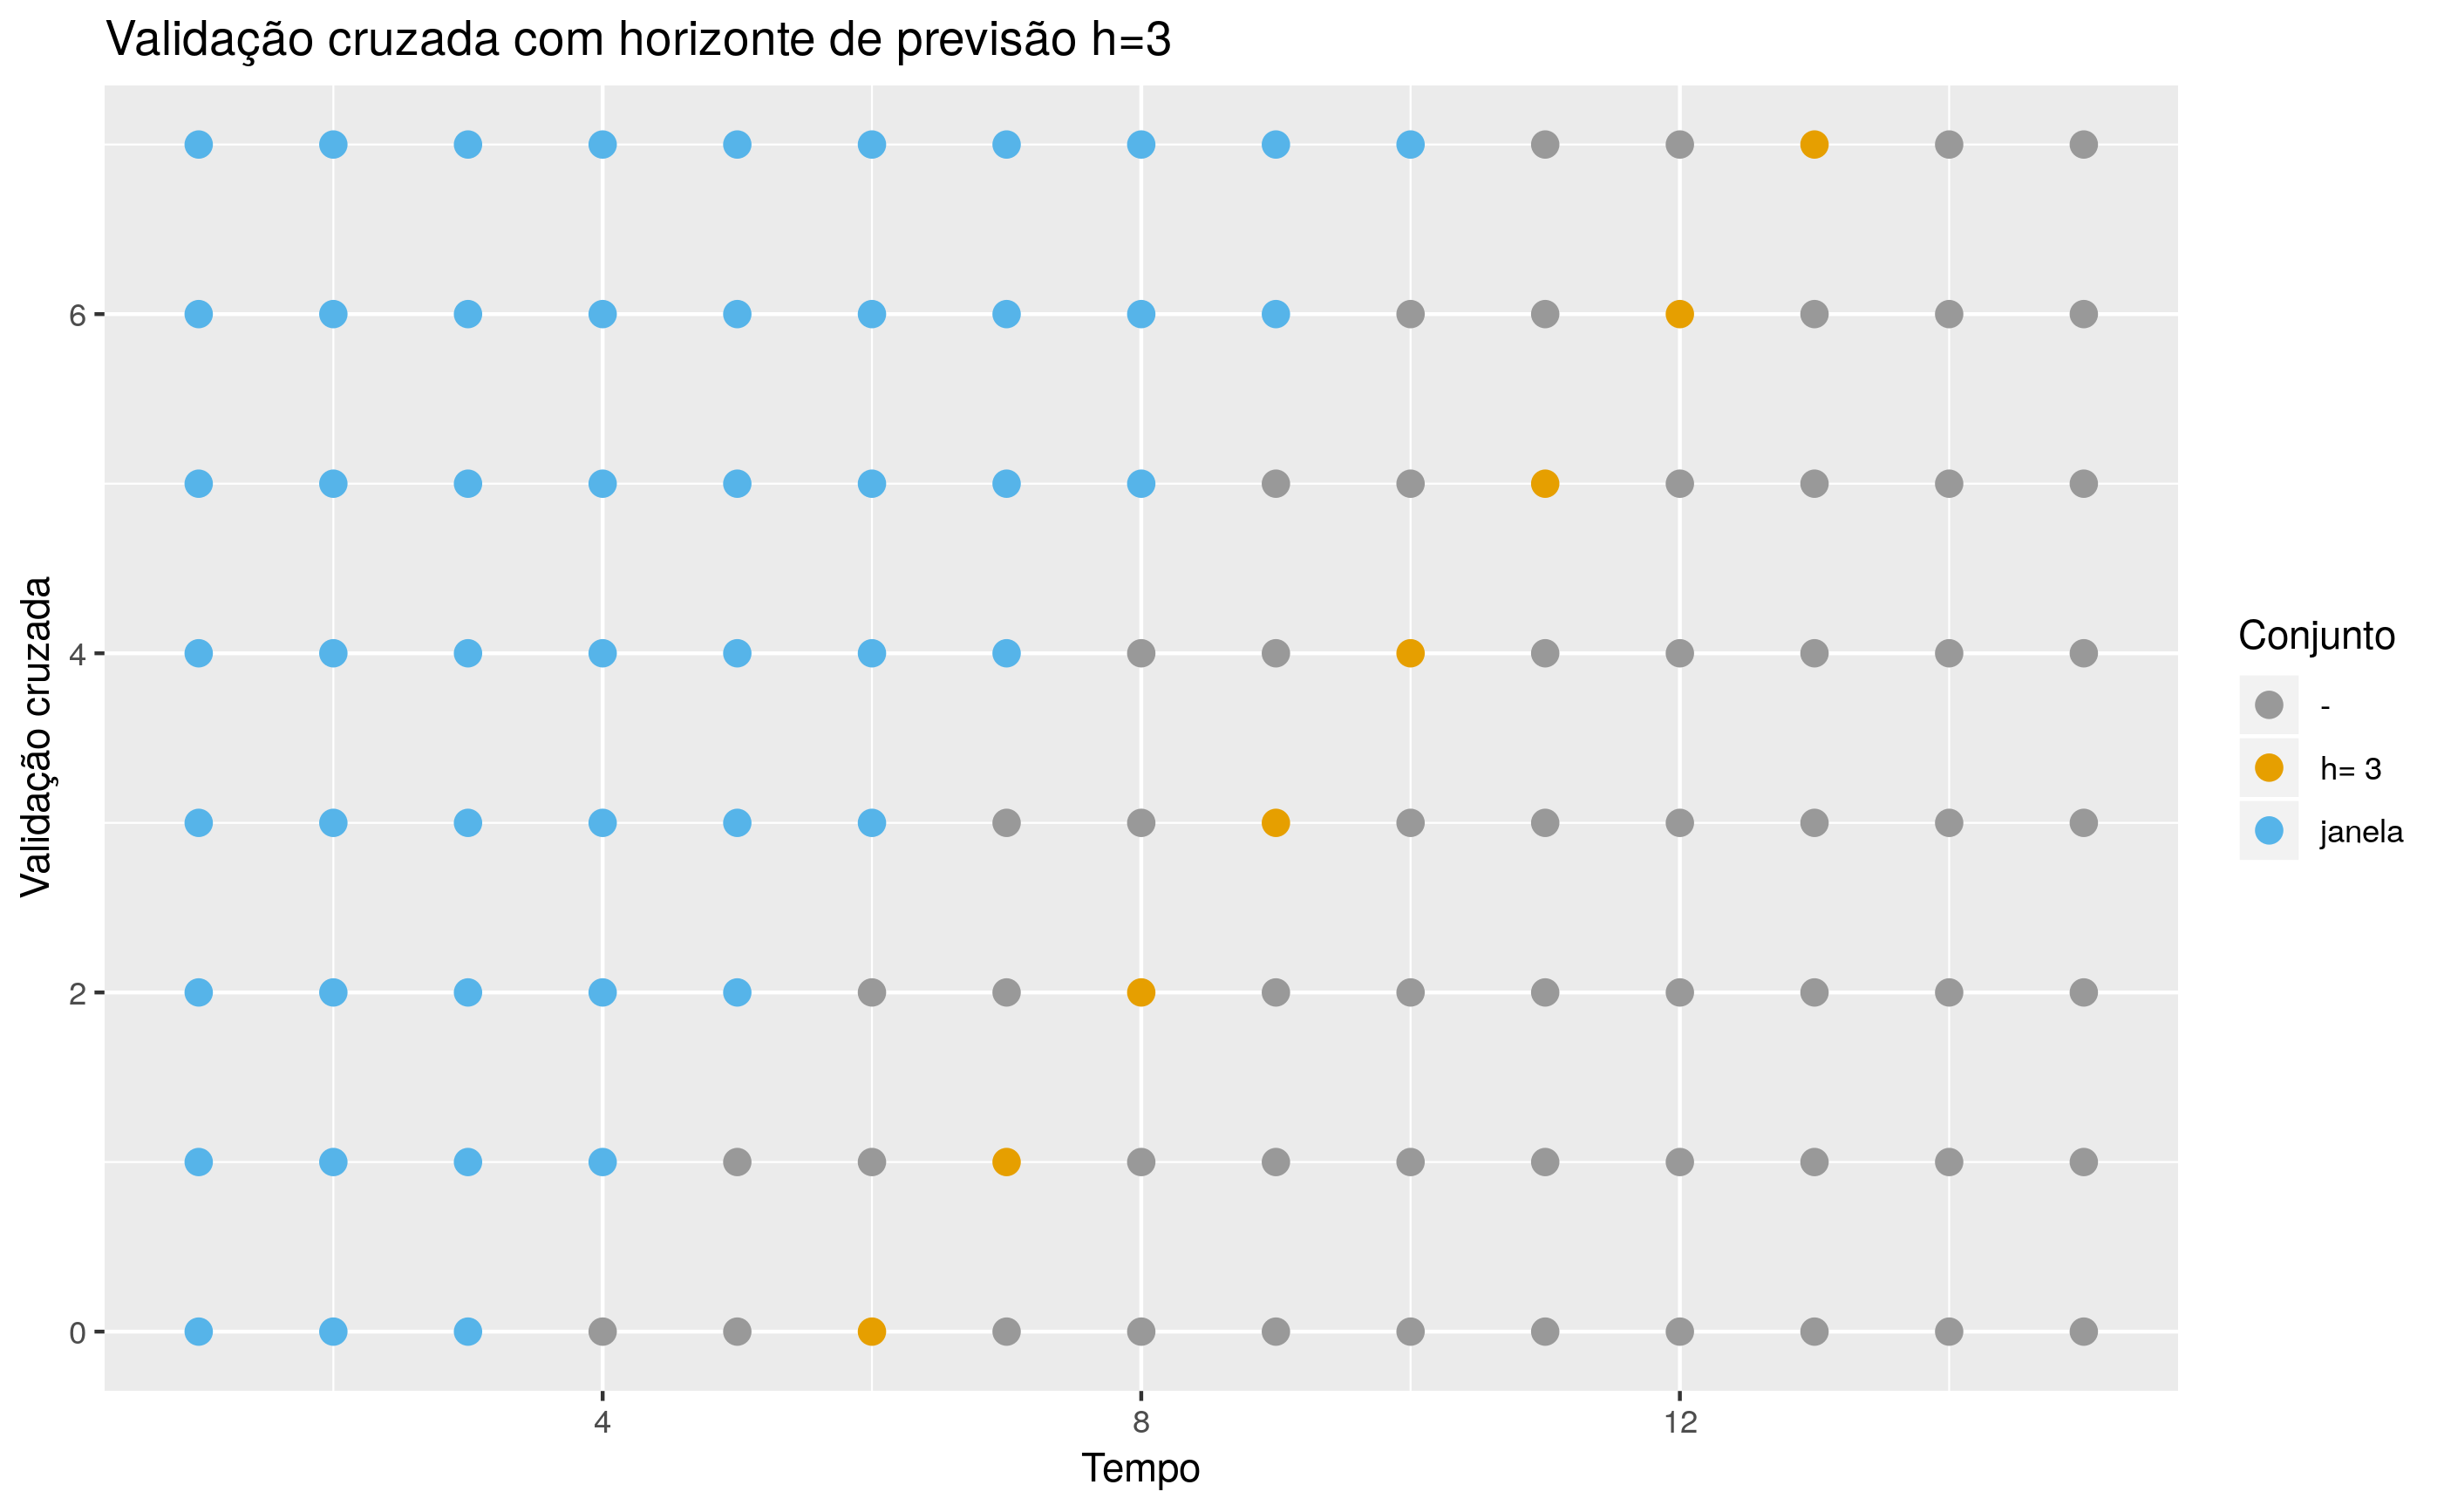
\includegraphics[width=\textwidth]{crossh3}
	\caption{Validação cruzada.}
\end{figure}
\FloatBarrier

Onde as medidas de treinamento estão em azul e as de teste em amarelo. Na linha de baixo, mensura-se o erro de previsão que resulta ao tentar prever três horas a frente da hora atual. A linha acima inclui a medida seguinte ao conjunto de treinamento e tenta prever, novamente, três horas a frente. Isso é feito várias vezes. Os erros resultantes são calculados, por exemplo, por MASE e a sua média é reportada como valor final. Em todos os testes de modelos que seguem as métricas reportadas são calculadas dessa forma.

\section{Estabilidade}

Os parâmetros p, d, q de modelos ARIMA não podem assumir quaisquer valores. Existem critérios de existência e estabilidade que basicamente garantem a convergência do polinômio que representam.

Um modelo ARIMA pode ser escrito da seguinte forma: 

%y^{'}_{t} = c + \phi_{1}y^{'}_{t-1} + \dots + \phi_{p}y^{'}_{t-p} + \theta_{1}\varepsilon_{t-1} + \dots + \theta_{q}\varepsilon_{t-q} + \varepsilon_{t}

\begin{equation}
\phi(B)(1-B)^dy_t = c + \theta(B)\varepsilon_t
\end{equation}

Sendo $d$ o grau de diferenciação aplicado, $\phi(B)$ é o polinômio de ordem $p$:

\begin{equation}
\phi(B) = (1-\phi_1B-\dots-\phi_pB^p)
\end{equation}

$\theta(B)$ é o polinômio de ordem $q$:

\begin{equation}
\theta(B) = (1+\theta_1B+\dots+\theta_qB^q)
\end{equation}

$B$ o operador definido por:

\begin{equation}
By_{t} = y_{t-1}
\end{equation}

A condição de regime estacionário de qualquer modelo ARIMA é de que as raízes complexas do polinômio $\phi(B)$ estejam fora do círculo unitário. Enquanto que a condição de invertibilidade é de que as raízes complexas de $\theta(B)$ estejam fora do círculo unitário. Pode-se verificar ambas as condições por meio do gráfico das raízes desses polinômios. Para facilitar a visualização, exibe-se o gráfico do respectivo polinômio inverso de tal forma que as condições sejam satisfeitas se as raízes estiverem dentro do círculo unitário.

\begin{figure}[h]
    \centering
	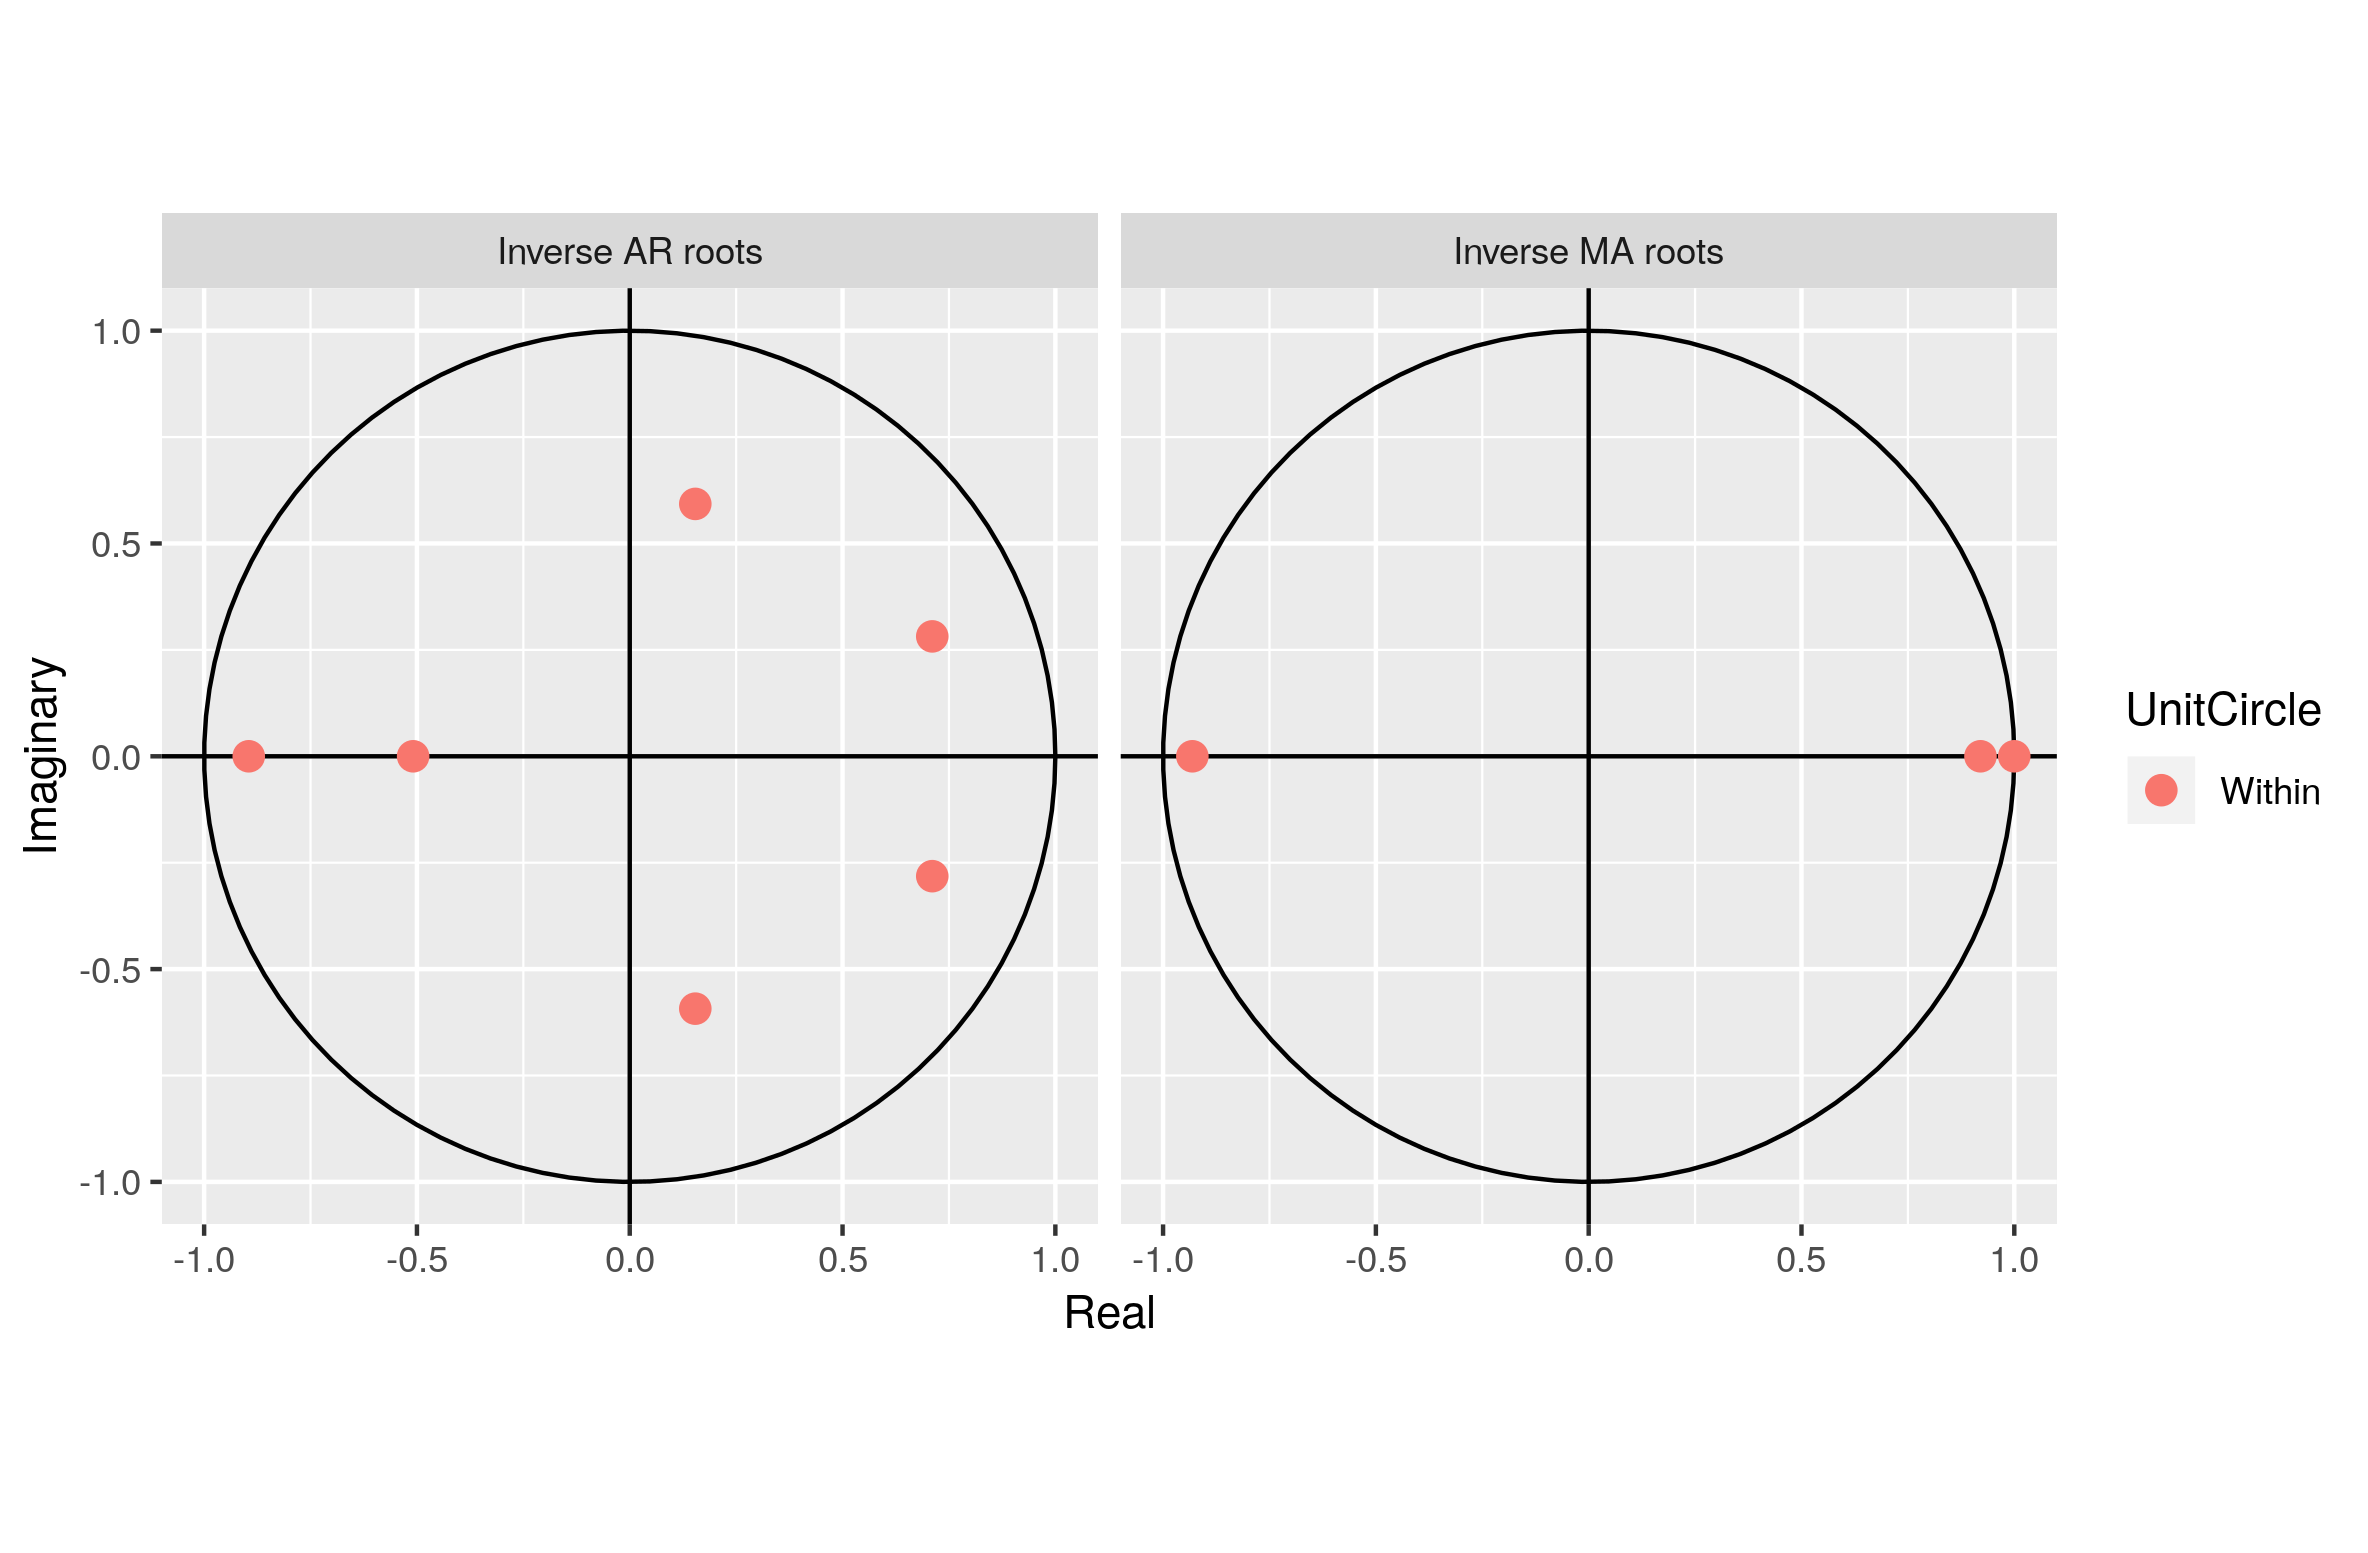
\includegraphics[width=\textwidth]{conds}
	\caption{Condições de regime estacionário e invertibilidade para um modelo ARIMA(6,1,3).}
\end{figure}
\FloatBarrier

\section{Previsão}

A estabilidade dos modelos propostos na seção \ref{janela} foi verificada e todas as raízes estão fora do círculo unitário. Dessa forma, pode-se comparar o desempenho de cada modelo atuando na série de dados. Para isso, foram utilizadas 2 semanas anteriores como conjunto de treino para estimar os parâmetros de cada modelo e a semana seguinte como conjunto de teste para comparar o que os modelos predizem com o que efetivamente foi registrado.

Visualmente a previsão pode ser demonstrada superpondo a curva prevista aos dados medidos. Esses modelos permitem que se calculem também intervalos de confiança. Optou-se por exibir os intervalos de 80\% e 95\% em azul escuro e claro, respectivamente. Um intervalo de 95\% indica que o modelo prevê com 95\% de confiança que o valor medido estará entre os limites indicados.

\begin{figure}[h]
    \centering
	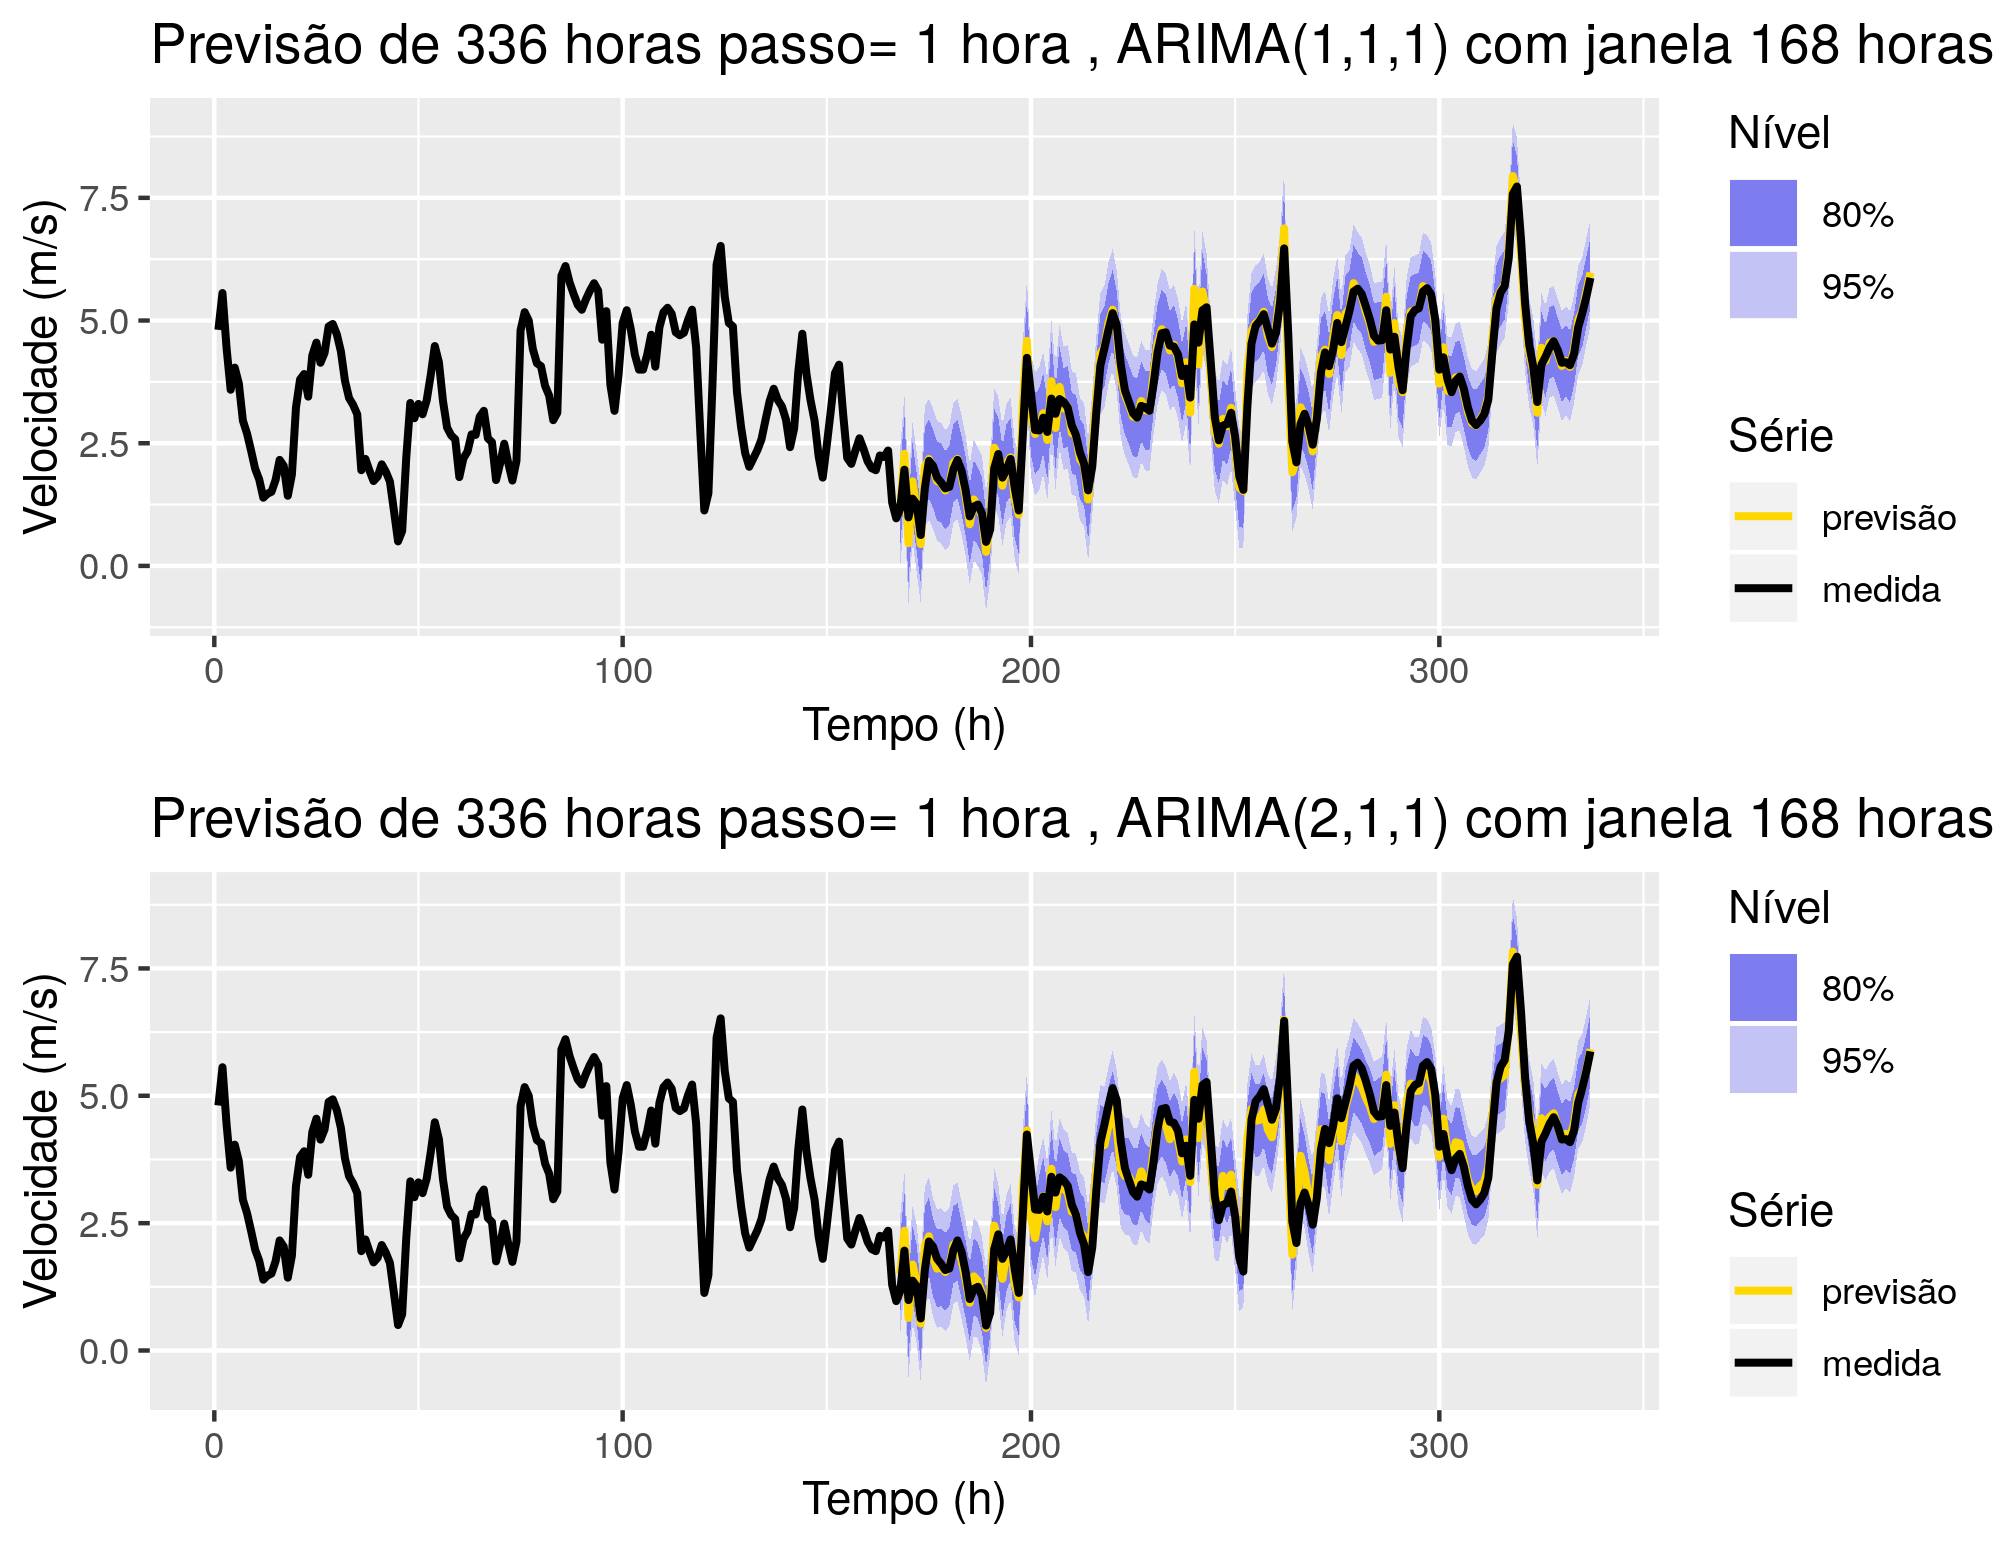
\includegraphics[width=\textwidth]{arima12}
	\caption{Previsão de velocidade do vento utilizando modelo ARIMA(1,1,1) (superior) e ARIMA(2,1,1) (inferior).}
\end{figure}
\FloatBarrier

\begin{figure}[h]
    \centering
	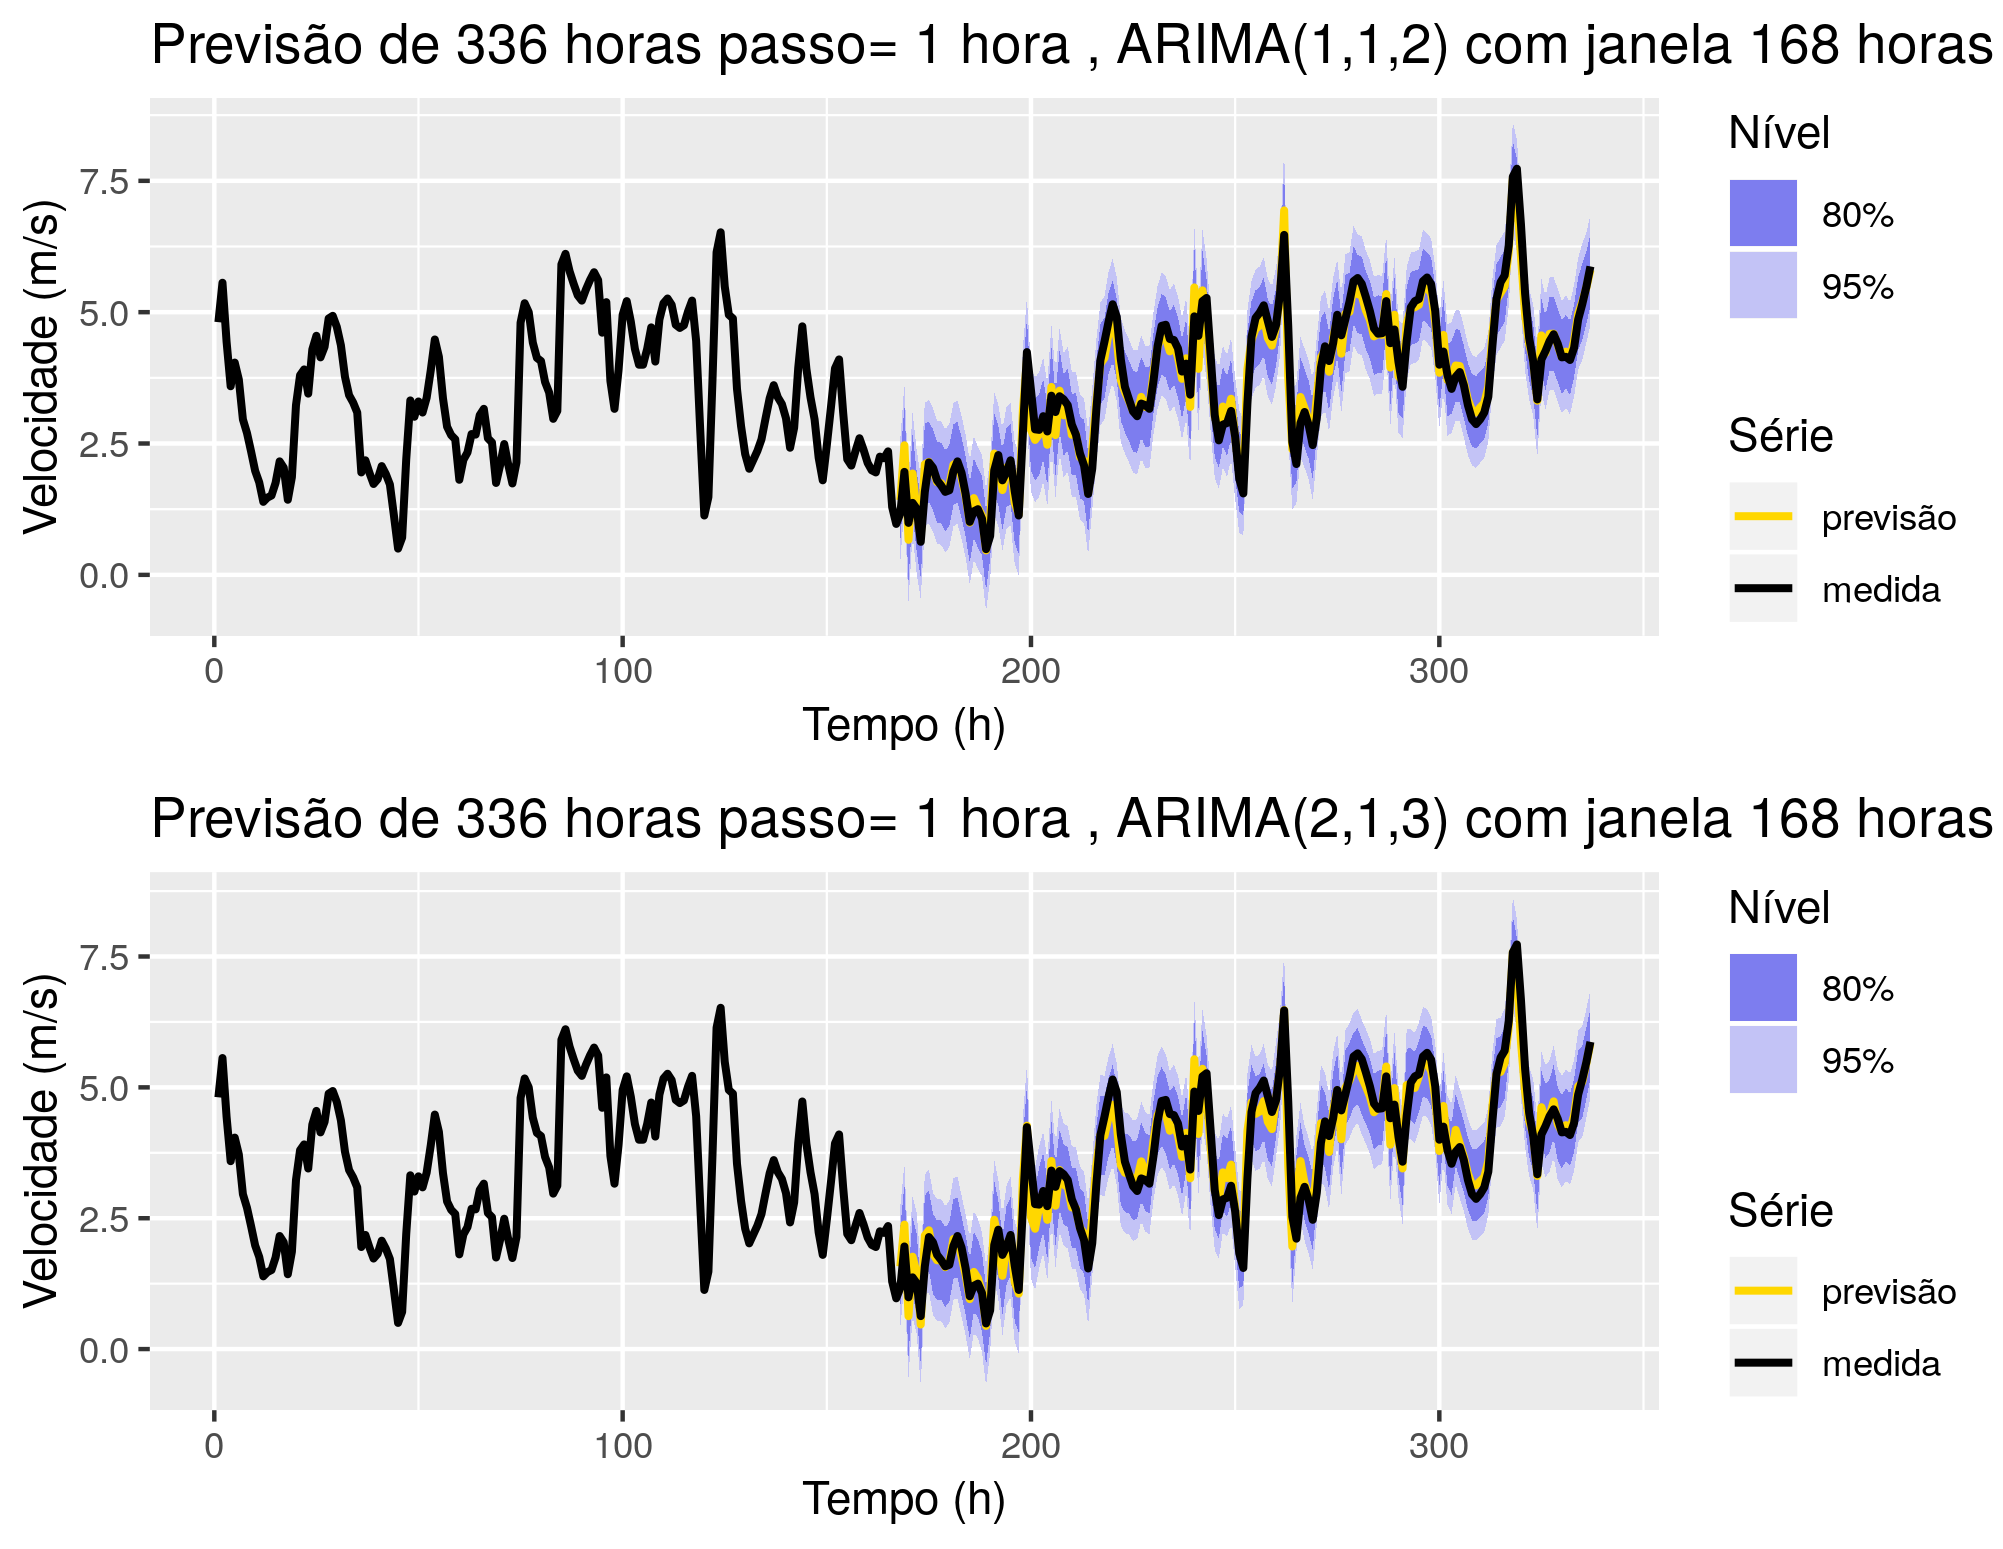
\includegraphics[width=\textwidth]{arima34}
	\caption{Previsão de velocidade do vento utilizando modelo ARIMA(1,1,2) (superior) e ARIMA(2,1,3) (inferior).}
\end{figure}
\FloatBarrier

Os valores quantitativas das diversas medidas de erro introduzidas na seção \ref{erro}, usando o procedimento de validação cruzada descrito em \ref{cruzada}.


\begin{table}[h]
\centering
\begin{tabular}{ |c|c|c|c|c|c| } 
\hline
\textbf{ARIMA(p,d,q)}&\textbf{ME}&\textbf{RMSE}&\textbf{MAE}&\textbf{MPE}&\textbf{MAPE}\\
\hline
1,1,1&-0.007948941&0.2231684&0.161981&0.3817872&5.731274 \\
\hline
2,1,1&0.00824027&0.2973698&0.2285103&-0.7558966&7.622429 \\
\hline
1,1,2&0.01559968&0.2490103&0.1870849&-0.8393794&6.151953 \\
\hline
2,1,3&0.01455176&0.3189862&0.2380204&-0.8382305&7.968127 \\
\hline
\end{tabular}
\caption{Medidas de erro para 4 modelos ARIMA aplicados à séries modelo.}
\end{table}

A minimização das métricas RMSE, MAE, MPE e MAPE sugere que o modelo ARIMA(1,1,1) apresenta melhor desempenho para essa janela de dados. No entanto, observa-se que esse modelo não fornece sempre os melhores resultados pra toda a extensão da série tampouco isso era esperado. A seção seguinte propõe um método de estimar continuamente os melhores parâmetros ARIMA para uma dada janela de dados.

%Apesar de o tempo de treinamento ser muito longo, mas 

%hat over predicted
%T+1|T
%
%A velocidade do vento é modelada por meio de um processo estocástico. Uma grandeza que é
%ideais da economia
%a diferença entre uma flutuação aleatória que não ocorrerá novamente e um padrão que deve ser modelado e extrapolado para o futuro
%Uma previsão nunca é estática, ela captura o modo pelo qual os dados estão mudando. Assume-se que esse modo é constante no tempo. É possível ainda reavaliar o modelo para que ele também se adapte a mudanças no modo 
%quanto mais longinquo o horizonte de previsão, quantas horas, dias, meses, anos no futuro, maior a incerteza na previsão e portanto mais abertos os intervalos de confiança'

\chapter{Modelo Autoregressivo Variável}

Ao longo do estudo observou-se que para diferentes períodos da série de dados, diferentes modelos ARIMA apresentavam melhor potencial preditivo não sendo possível elencar um único modelo que capturasse a estrutura da série de forma universal. Duas soluções para esse problema foram exploradas. Uma delas é optar por outro modelo. A outra, abordada nessa seção, é permitir que os parâmetros ARIMA fossem adaptativos, sendo recalculados, a medida que mais dados são coletados.
%Uma possível solução para 
Essa é uma estratégia interessante por vários motivos. É possível estimar os parâmetros de um modelo ARIMA rapidamente de forma que a previsão esteja disponível ininterruptamente mesmo em escalas temporais da ordem de minutos. Qualquer mudança estrutural na grandeza física de interesse é automaticamente capturada pelo modelo, como, por exemplo, um aumento na turbulência devido a um aumento da temperatura média do planeta.

A imagem abaixo exibe a evolução temporal dos graus de liberdade do modelo em um espaço de fase sendo possível entender como os parâmetros variam ao longo do tempo e consequentemente como a estrutura dos dados (limitada pela representação por um modelo ARIMA) varia. O tempo é representado pela escala em cor. O parâmetro de diferenciação, d, do modelo assume, durante quase todo o período, o valor 1 e, portanto, exibe-se apenas os parâmetros p e q.

\begin{figure}[h]
    \centering
	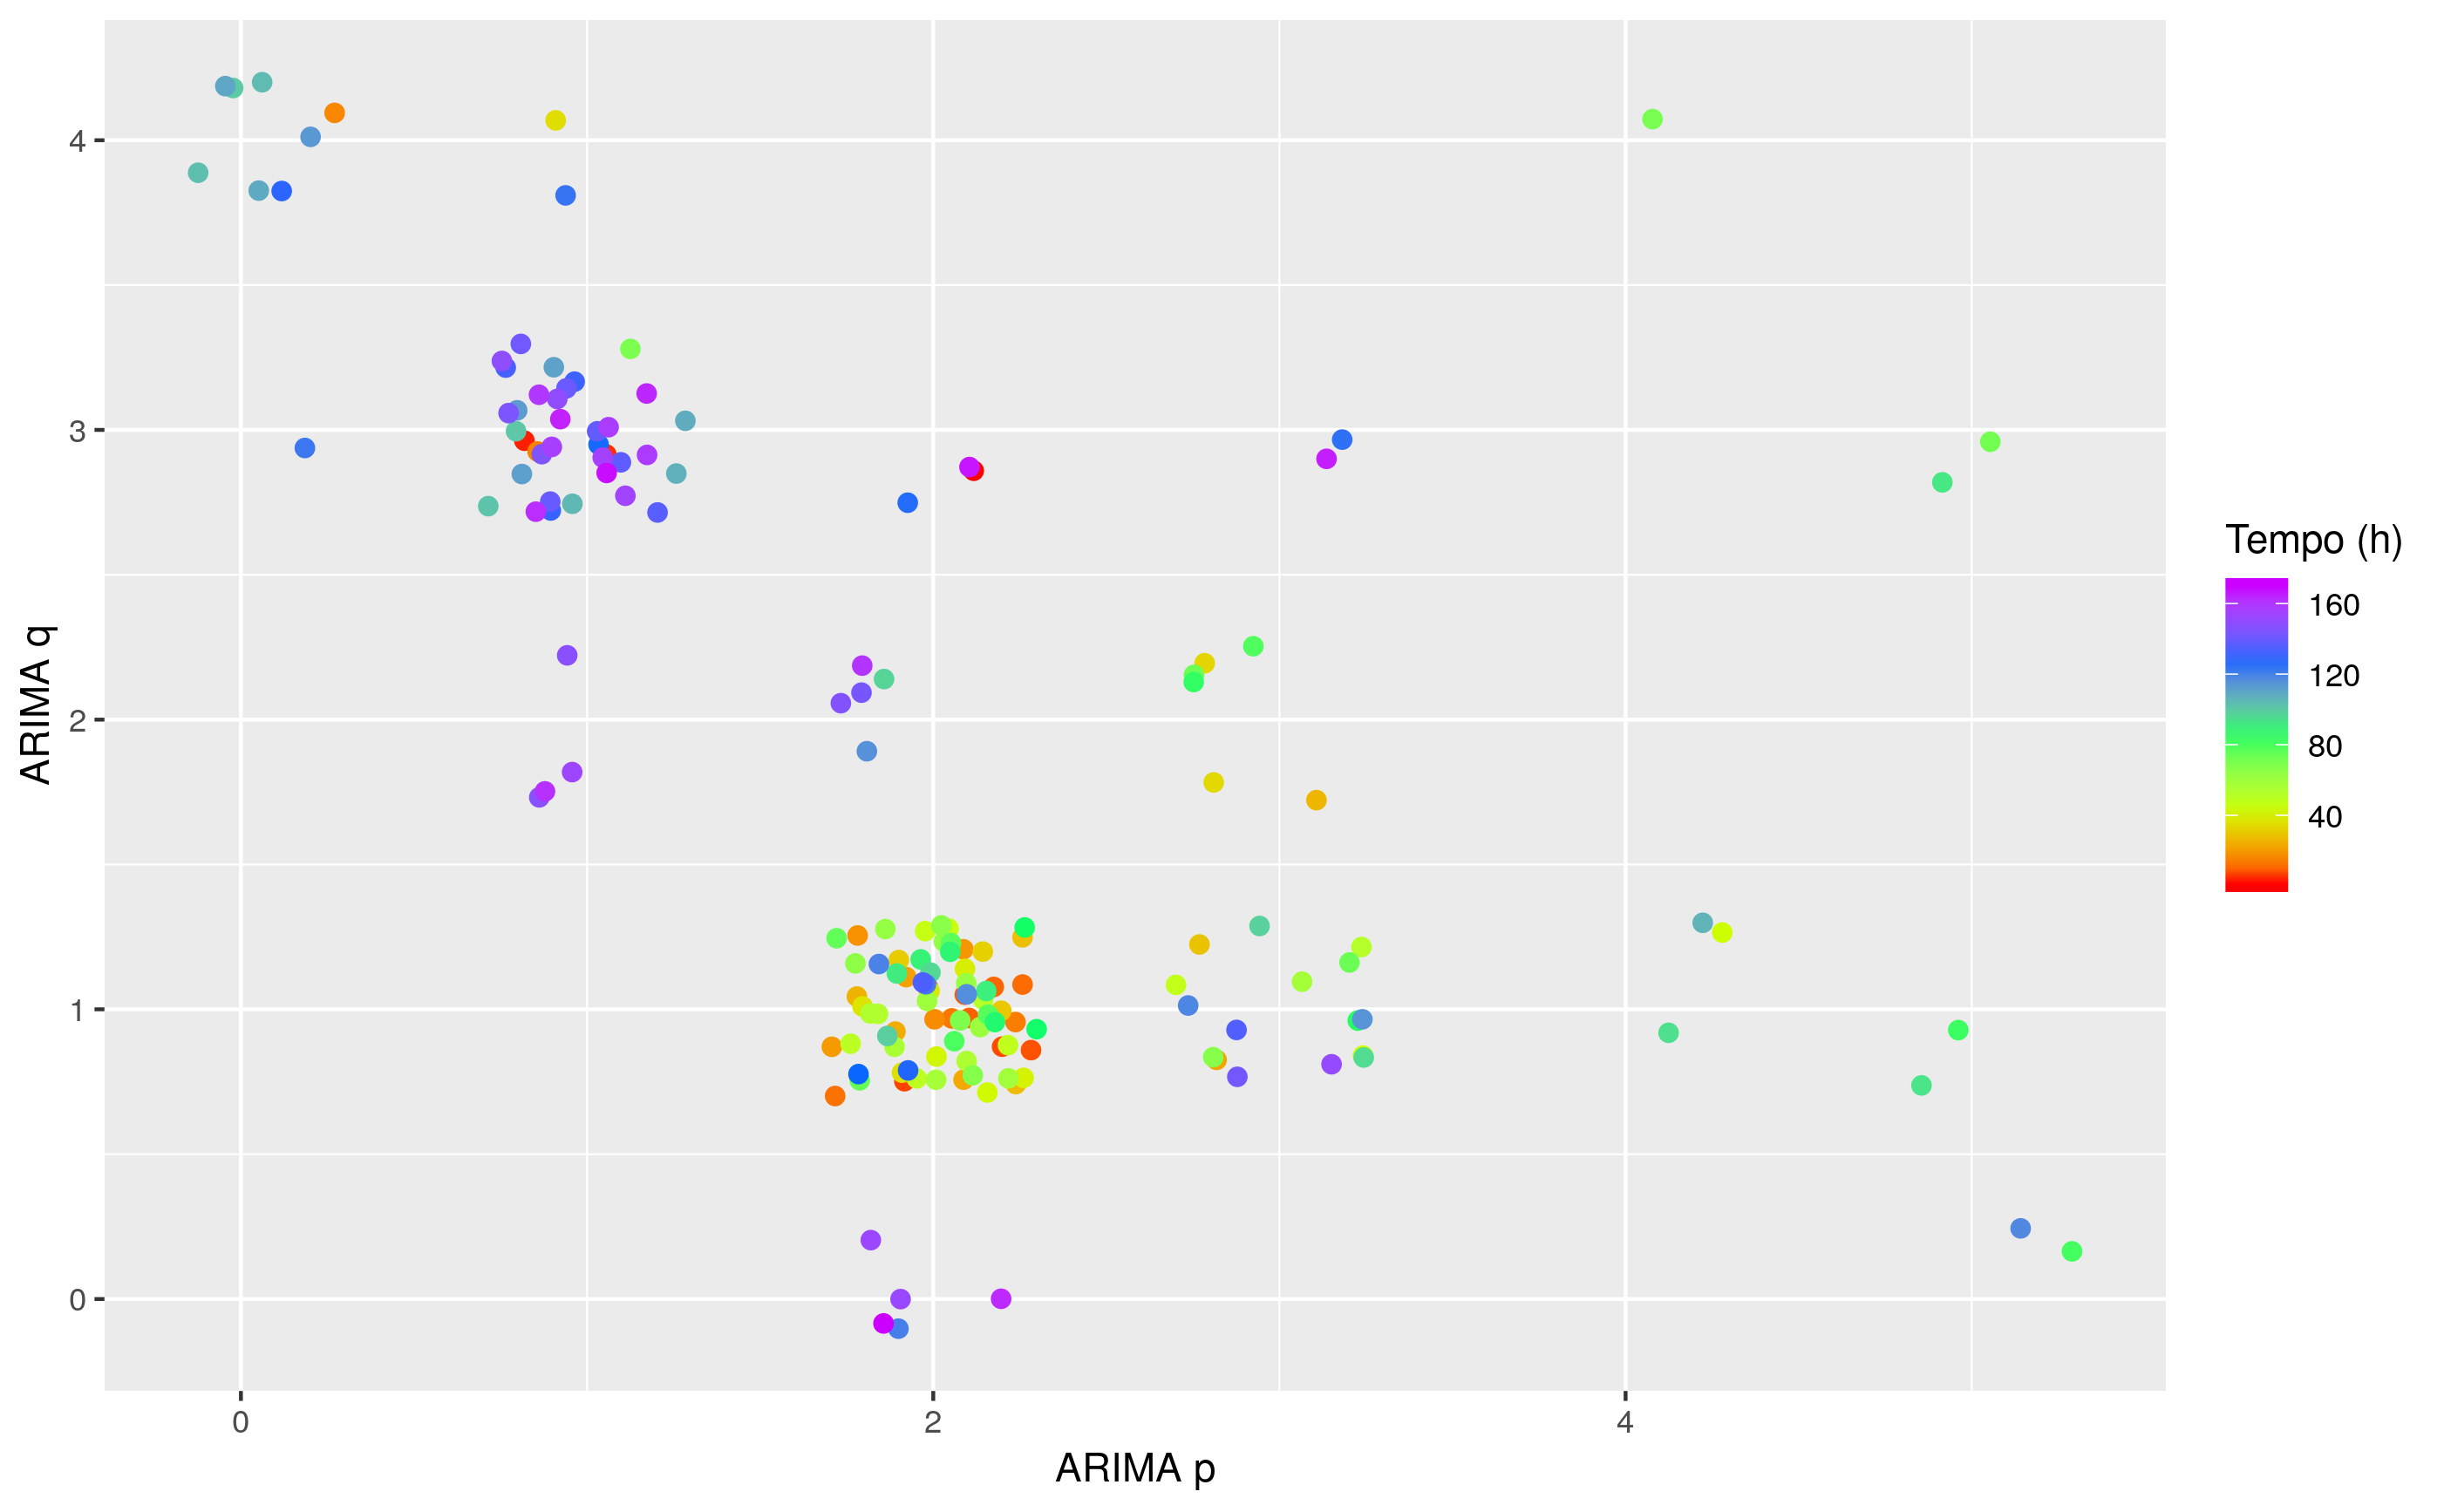
\includegraphics[width=\textwidth]{var_arima}
	\caption{Evolução dos parâmetros p e q de um modelo ARIMA ao longo do tempo.}
\end{figure}
\FloatBarrier

Modelos ARIMA são definidos pelos parâmetros $p$,$d$,$q$. O parâmetro $p$ representa o número de termos anteriores da série que influenciam o valor atual. Os pesos com que cada termo anterior contribui para a estimativa do valor seguinte são parâmetros a serem estimados por regressão linear.
O parâmetro q tem um papel análogo ao do parâmetro q. Ele refere-se a inclusão dos q erros anteriores na estimativa do valor seguinte.

Os parâmetros assumem apenas valores inteiros. Para facilitar a visualização da evolução temporal adicionou-se um ruído aleatório a cada ponto de modo a evitar a sua sobreposição. Fica claro que no início do período de 160 horas o principal modelo ARIMA é o ARIMA(2,1,1) enquanto que ao final do período o modelo preferencial é o ARIMA(1,1,3). Também observa-se que diversos outros modelos são assumidos com menos frequência.

Apesar do apelo prático, o método não se mostrou satisfatório:

%No entanto, apesar do forte apelo intuitivo e melhora no poder preditivo

\begin{figure}[h]
    \centering
	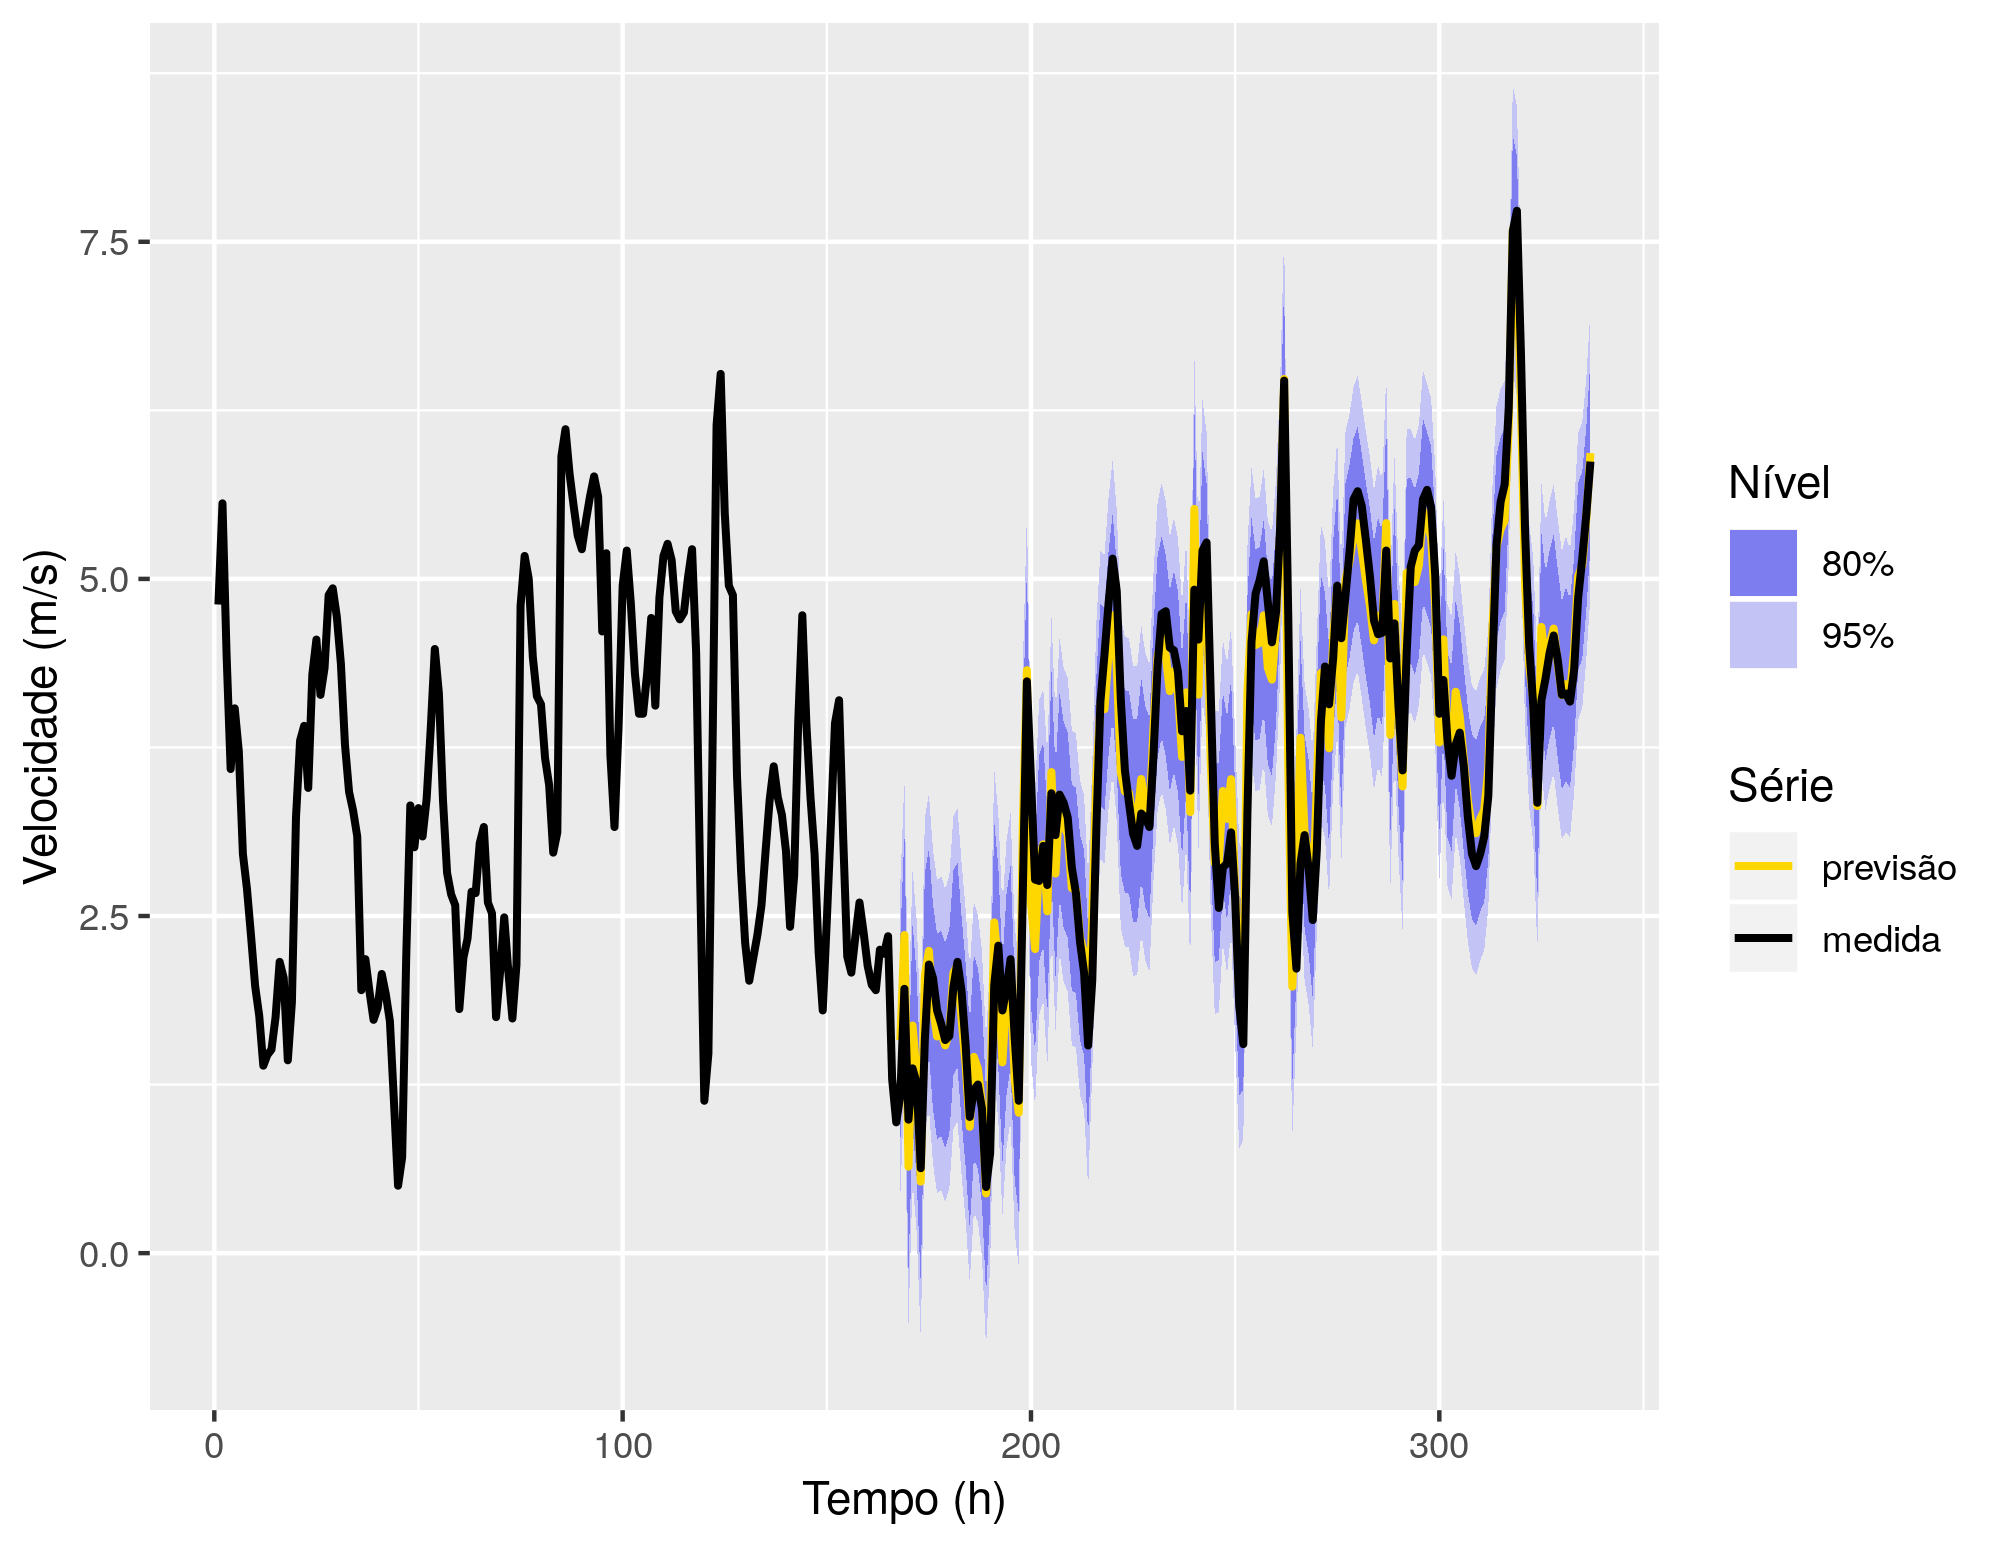
\includegraphics[width=\textwidth]{var_result}
	\caption{Previsão resultante do modelo ARIMA com parâmetros variáveis.}
\end{figure}
\FloatBarrier

\chapter{GARCH}

Séries de dados de vento possuem uma característica fundamental em comum que não foi modelada até então: sua variância não é constante. Os esforços dispendidos foram no sentido de neutralizar a variância. Além disso, o comportamento da variância em séries de velocidade do vento é mais simples, ao contrário de séries financeiras.

\section{Base horária}

Em base horária os períodos de maior e menor variância são facilmente previsíveis e possuem uma interpretação física clara. Períodos de variância elevada são observados durante períodos de simultânea alta temperatura do ar, o que o torna mais turbulento e, portanto, aumenta a variabilidade das medições, enquanto que, à noite, por exemplo, a atmosfera próxima ao solo se estratifica em camadas bem definidas e comportadas em um regime laminar, longe da turbulência e de tal forma apresentam baixa variabilidade.

\begin{figure}[h]
    \centering
	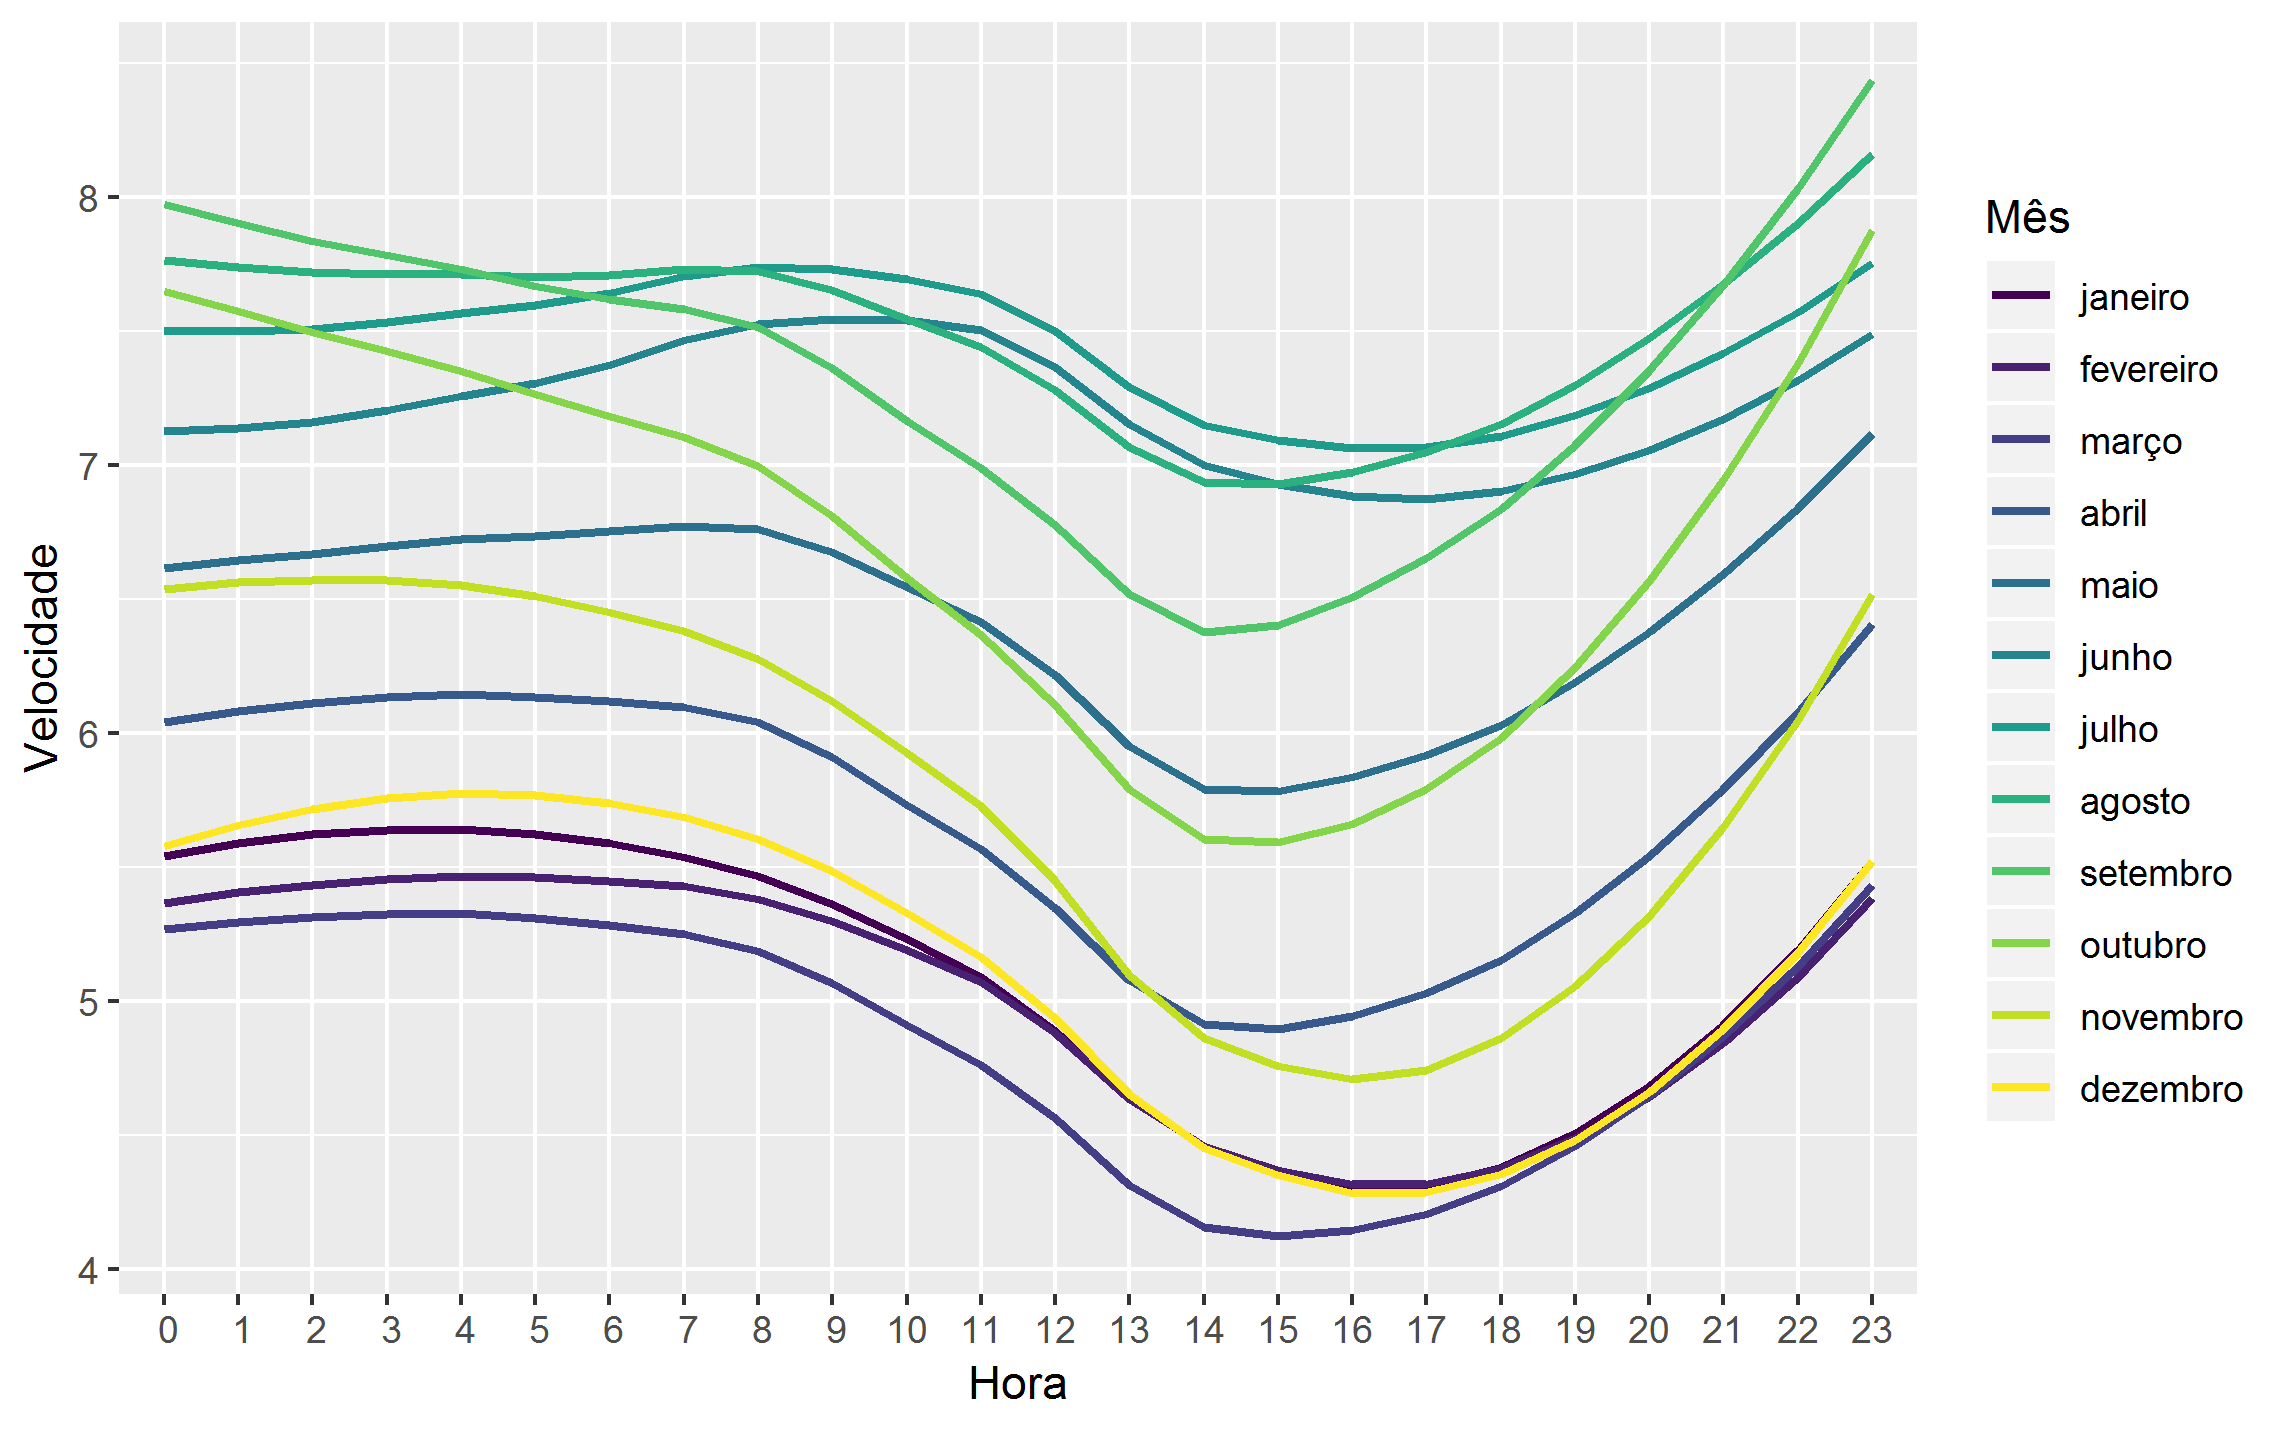
\includegraphics[width=\textwidth]{diurnal}
	\caption{Variação da velocidade por hora do dia. Uma curva por mês.}
\end{figure}
\FloatBarrier

O modelo autorregressivo de heterocedasticidade (variância) condicional (ARCH), proposto por Engle, \cite{engle} estende o modelo ARIMA modelando a variação na variância da série temporal. Este modelo faz uso de muitos parâmetros para produzir bons resultados. A generalização do método ARCH, proposta por Tim Bollerslev \cite{boller} conduz a modelos parcimoniosos, com menos parâmetros. Em um modelo GARCH a variância é modelada por:

\begin{equation}\label{eq61}
\sigma_t^2 = \underbrace{\beta_1\sigma_{t-1}^2 + \dots + \beta_p\sigma_{t-p}^2}_\text{autorregressão}  + \underbrace{\omega + \alpha_1\varepsilon_{t-1}^2 + \dots + \dots \alpha_q\varepsilon_{t-q}^2}_\text{média móvel} 
\end{equation}

\begin{equation}
\sigma_t^2 = \sum\limits_{i=1}^q\beta_i\sigma_{t-i}^2 + \omega + \sum\limits_{i=1}^q\alpha_i\varepsilon_{t-i}^2
\end{equation}

A equação \ref{eq61} deixa claro a analogia entre um modelo ARIMA e um GARCH. ARIMA aplica um filtro na própria série enquanto GARCH aplica na sua variância. Os resultados desse modelo são exibidos abaixo:

\begin{figure}[h]
    \centering
	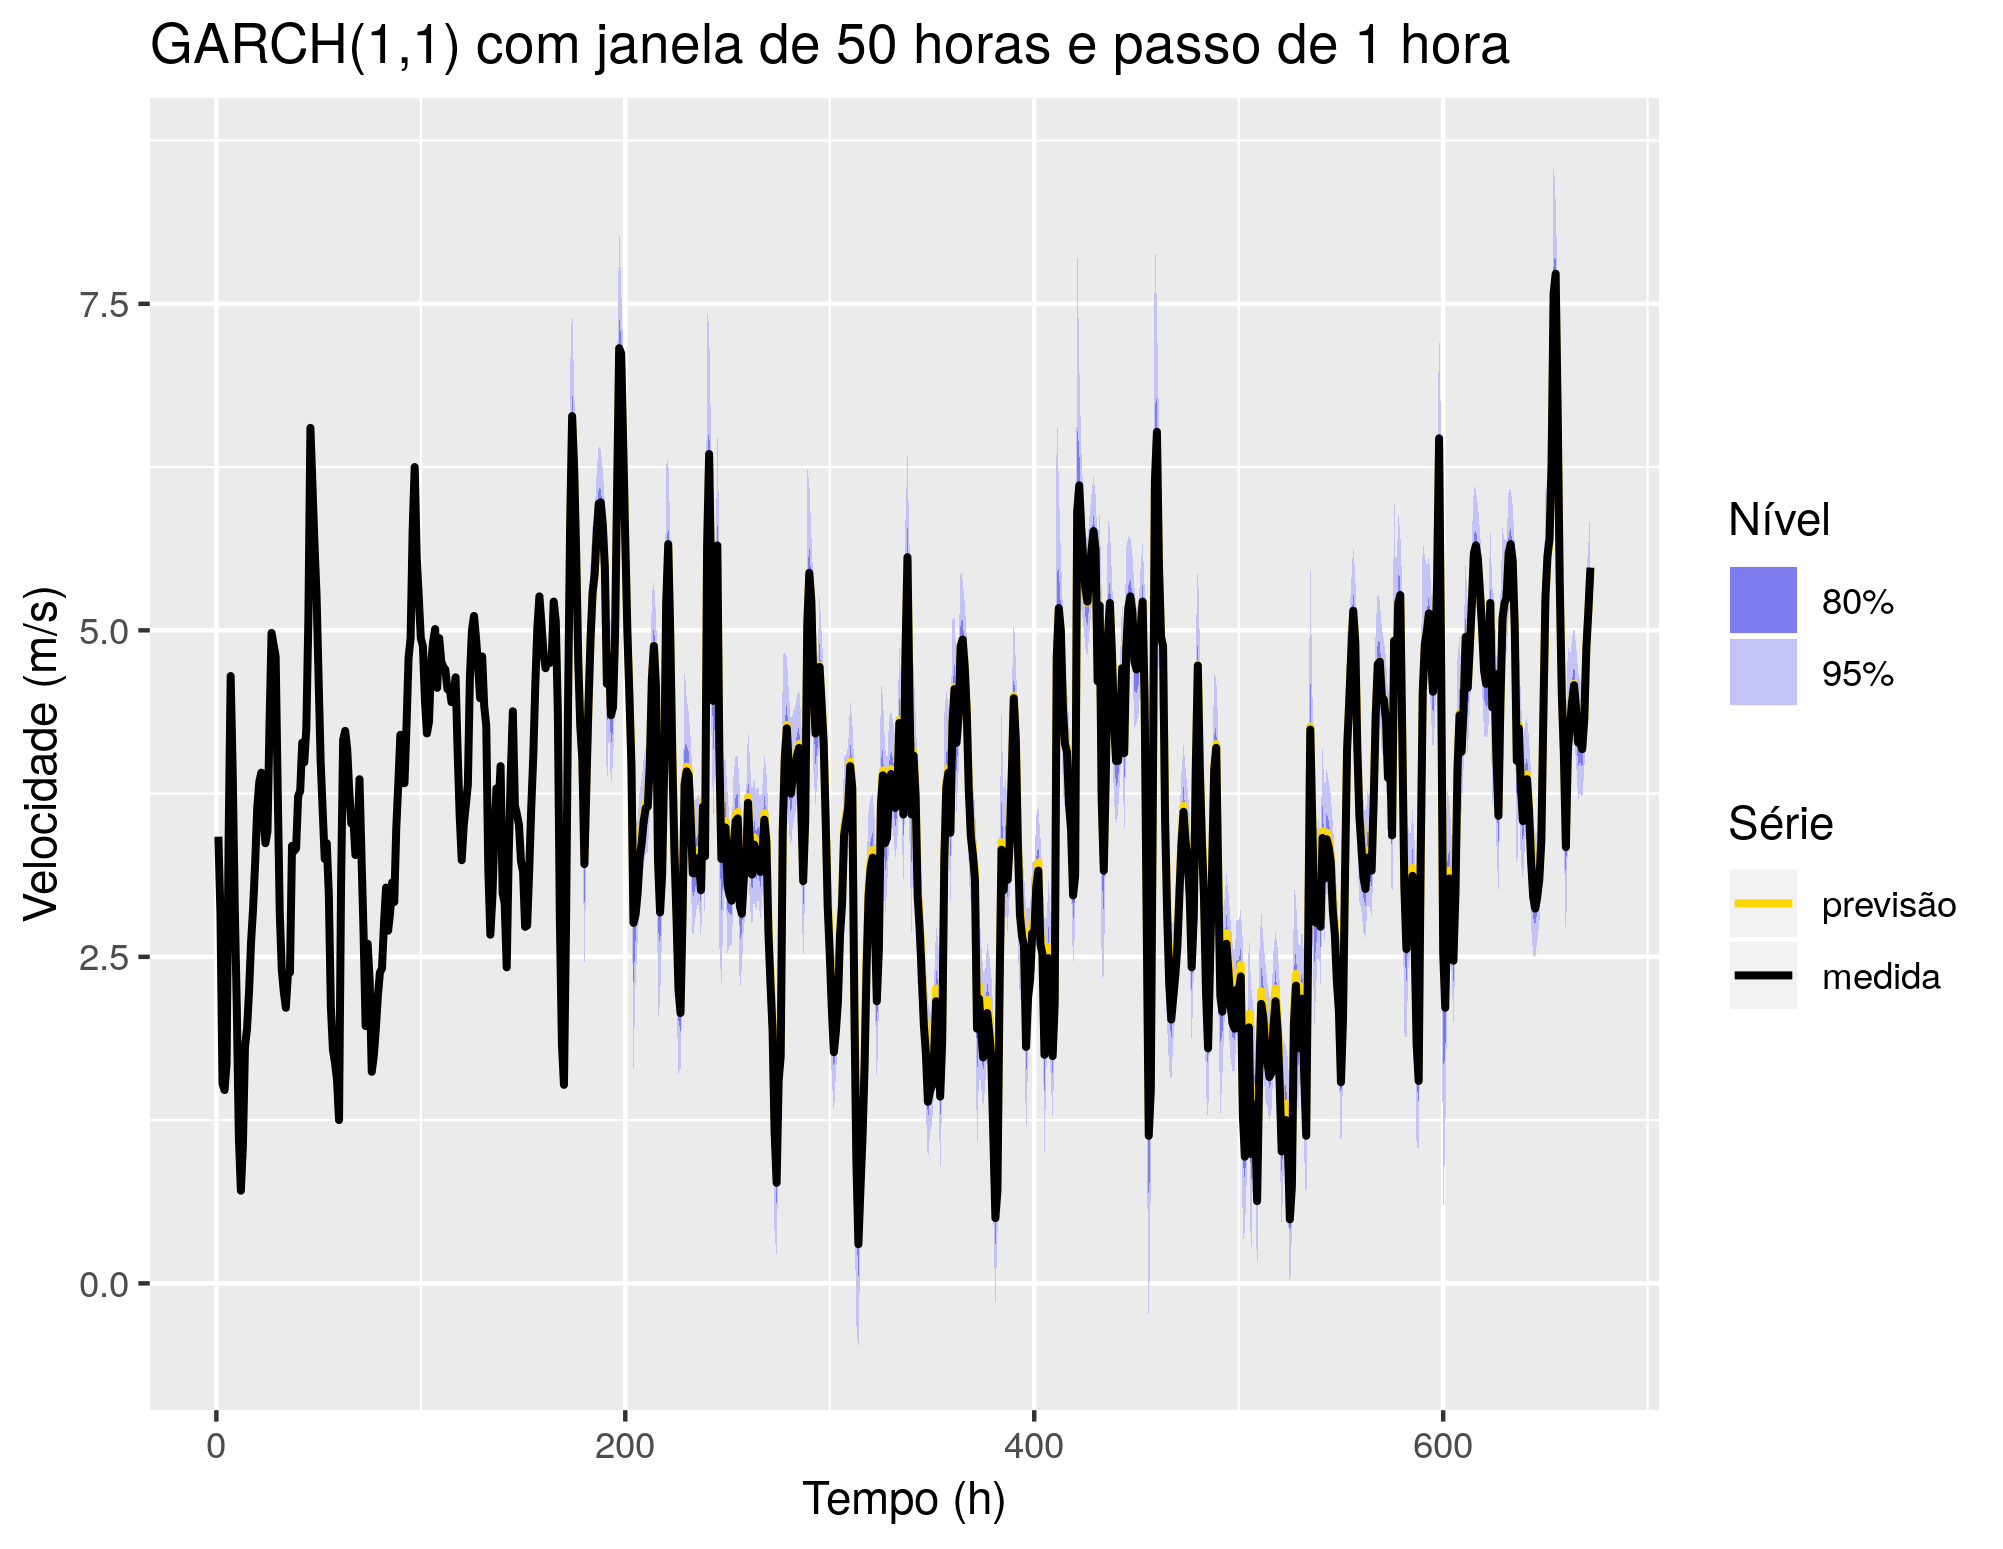
\includegraphics[width=\textwidth]{garch_first}
	\caption{Previsão da série modelo utilizando GARCH(1,1) em base horária.}
	\label{fig:garch}
\end{figure}
\FloatBarrier

\begin{table}[h]
\centering
\begin{tabular}{ |c|c|c|c|c|c| } 
\hline
\textbf{Modelo}&\textbf{ME}&\textbf{RMSE}&\textbf{MAE}&\textbf{MPE}&\textbf{MAPE}\\
\hline
GARCH(1,1)&-0.04246845&0.06505767&0.05117909&-2.449632&2.592525 \\
\hline
ARIMA(1,1,1)&-0.007948941&0.2231684&0.161981&0.3817872&5.731274 \\
\hline
ARIMA(2,1,1)&0.00824027&0.2973698&0.2285103&-0.7558966&7.622429 \\
\hline
ARIMA(1,1,2)&0.01559968&0.2490103&0.1870849&-0.8393794&6.151953 \\
\hline
ARIMA(2,1,3)&0.01455176&0.3189862&0.2380204&-0.8382305&7.968127 \\
\hline
\end{tabular}
\caption{Comparação de medidas de erro entre o modelo GARCH(1,1) e modelos ARIMA utilizados anteriormente.}
\end{table}

\section{Base mensal}

Embora a previsão horária seja de grande utilidade tanto para operadores de parques eólicos quanto para operadores de subestações de distribuição de energia, contratos de produção e entrega de energia são feitos em base mensal. Dessa forma, um acionista de um parque eólico deseja saber em qual nível de produção ele pode arriscar se comprometer em entregar em um acordo fechado um mês antes. O mesmo modelo, GARCH(1,1), se demonstra novamente adequado:

\begin{figure}[h]
    \centering
	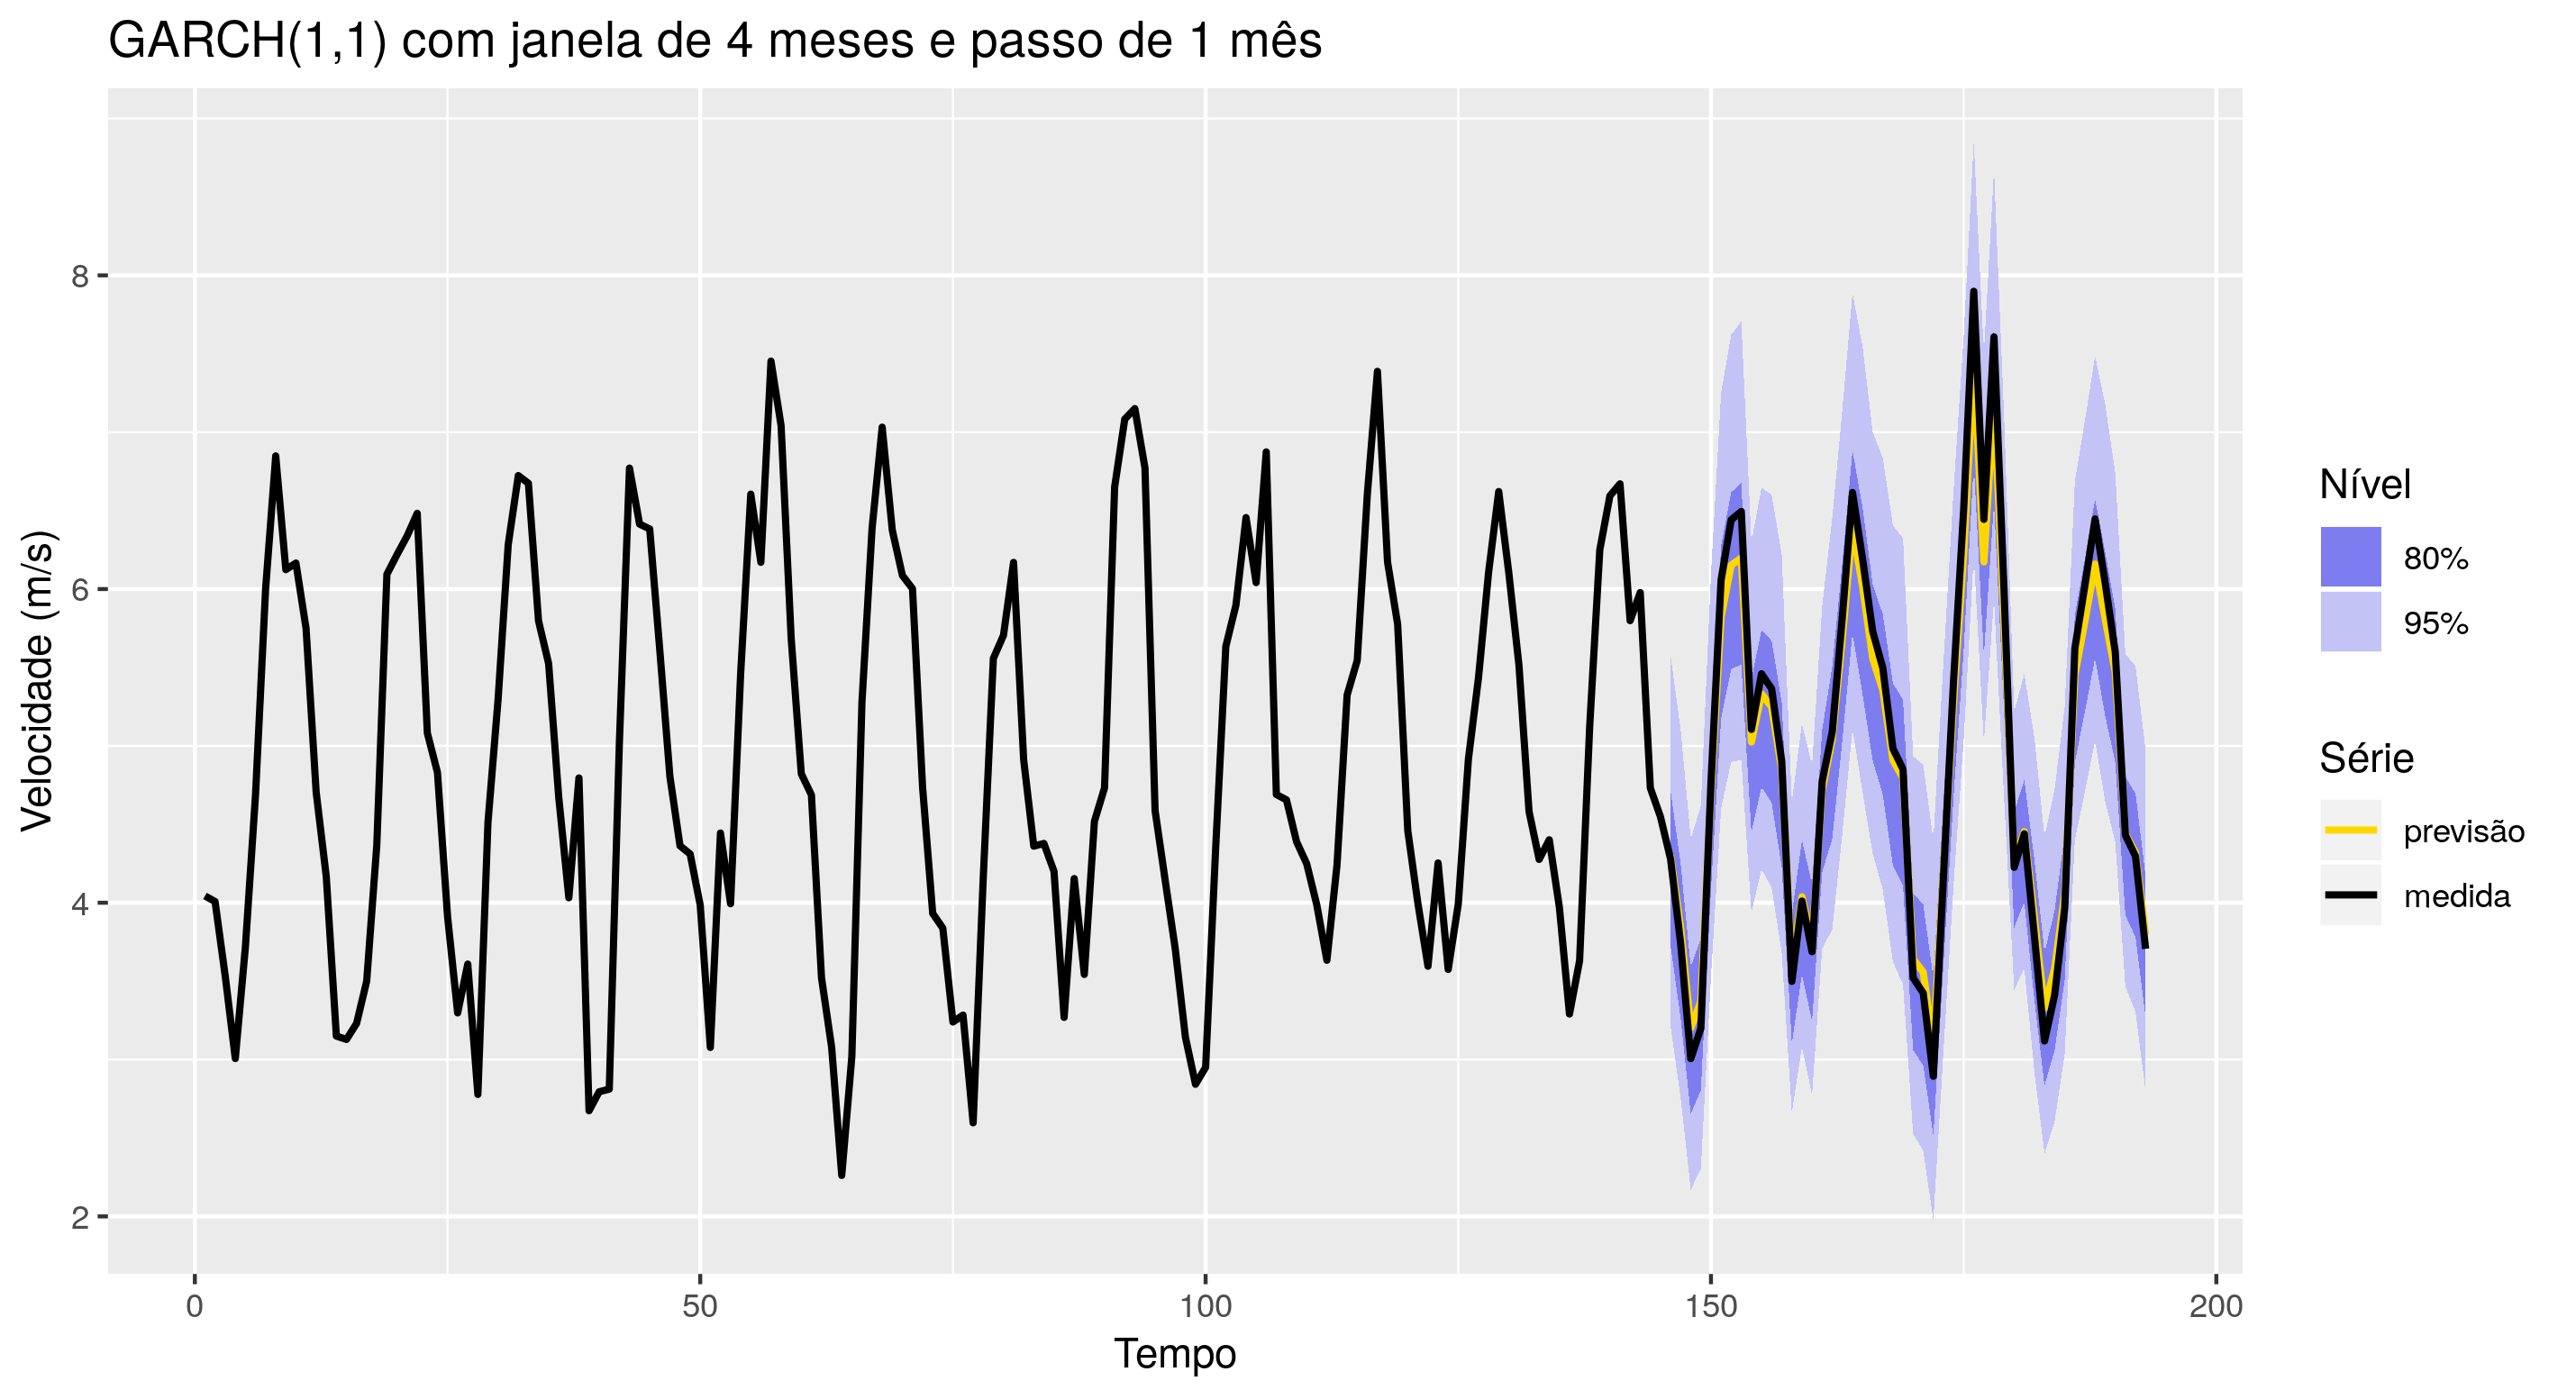
\includegraphics[width=\textwidth]{garch_month_edited}
	\caption{Previsão da série modelo utilizando GARCH(1,1) em base mensal.}
\end{figure}
\FloatBarrier

\begin{table}[h]
\centering
\begin{tabular}{ |c|c|c|c|c|c| } 
\hline
\textbf{Modelo}&\textbf{ME}&\textbf{RMSE}&\textbf{MAE}&\textbf{MPE}&\textbf{MAPE}\\
\hline
GARCH(1,1)&0.06669541&0.1773425&0.1461843&0.5504064&2.893245\\
\hline
\end{tabular}
\caption{Medidas de erro para o modelo GARCH(1,1) em base mensal.}
\end{table}

\part{Conclusão}

\chapter{Conversão em energia}

De acordo com a equação \ref{eq:1} a potência desenvolvida por um aerogerador é função principalmente da área coberta pelas suas pás, da densidade local do ar e do cubo da velocidade do vento. Exceto pela velocidade do vento os demais parâmetros variam pouco. Dessa forma, uma vez definidos os outros parâmetros, é possível obter a potência desenvolvida por um aerogerador por meio de sua curva de potência que mapeia intervalos de velocidade em intervalos de potência. A figura abaixo é um exemplo de curva de potência genérica (adaptada de \cite{pccurve}):

\begin{figure}[h]
    \centering
	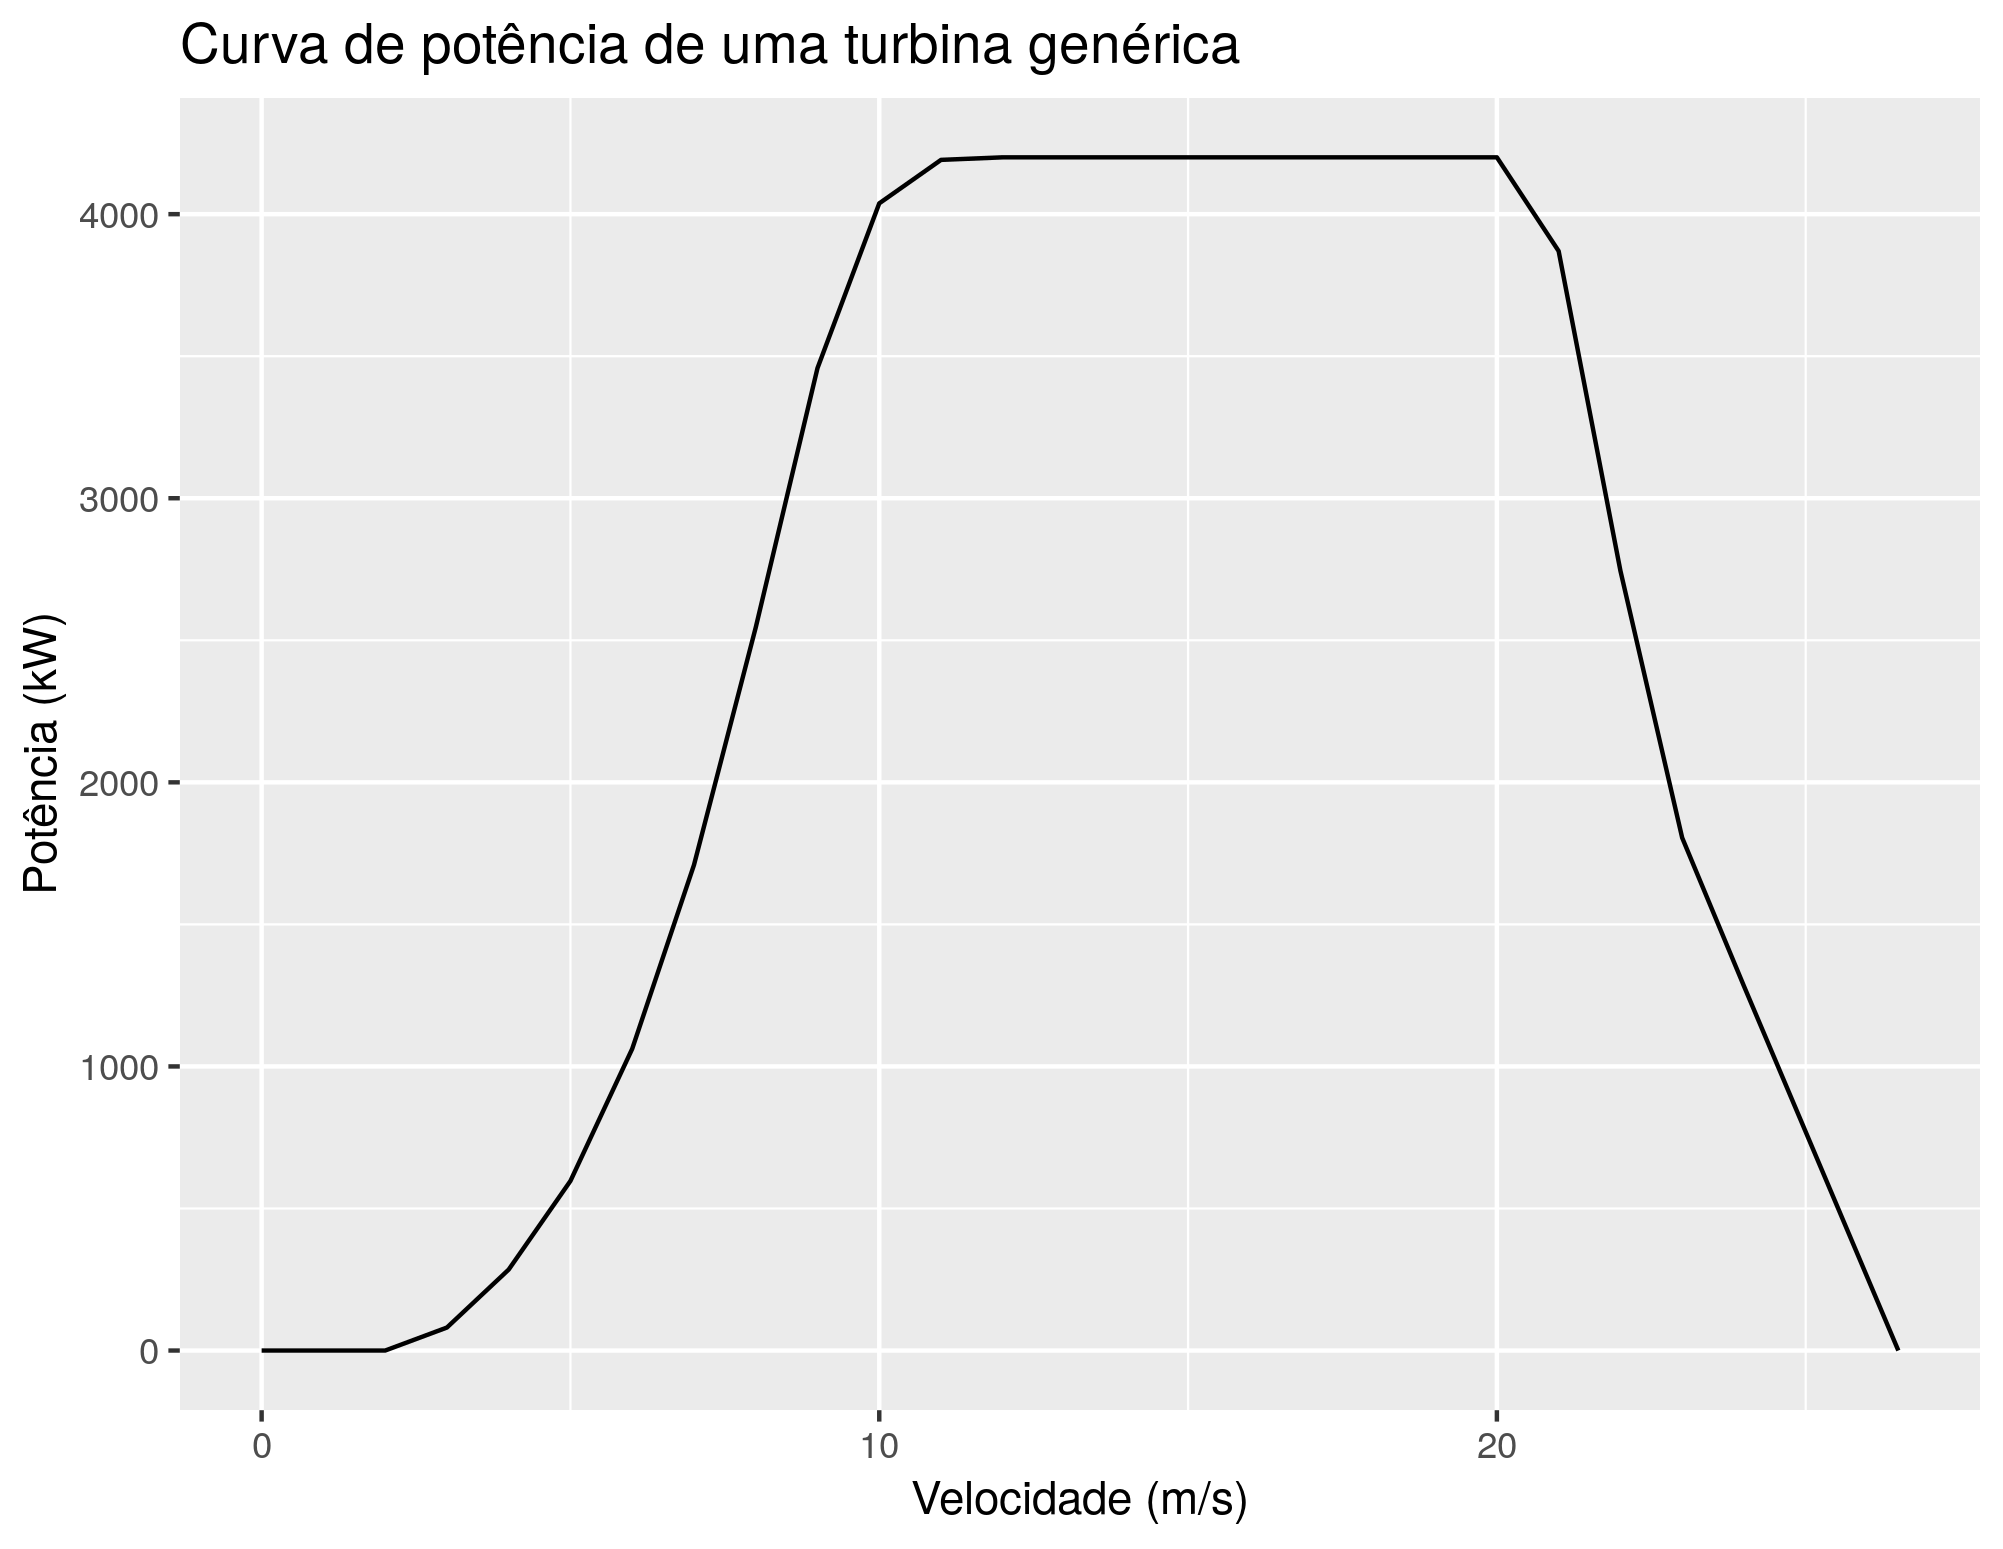
\includegraphics[width=\textwidth]{power_curve}
	\caption{Curva de potência de uma turbina genérica.}
\end{figure}
\FloatBarrier

As curvas de potência de qualquer turbina eólica possuem esse formato característico. A turbina só produz energia a partir de uma certa velocidade mínima. Para velocidades mais altas encontra uma região linear, onde a potência aumenta linearmente com a velocidade. Para uma certa velocidade chega-se num plateau de potência acima do qual um aumento de velocidade não causa variação na potência. Para velocidades muito altas é necessário desacelerar a rotação das pás de modo a não danificar componentes do aerogerador e portanto a potência decai. Quando a velocidade excede um valor limite é necessário desligar o aerogerador.

O mapeamento entre velocidade e potência é exibido abaixo. A série temporal de velocidade do vento corresponde àquela para a qual foi feita a previsão em 	\ref{fig:garch}.

\begin{figure}[h]
    \centering
	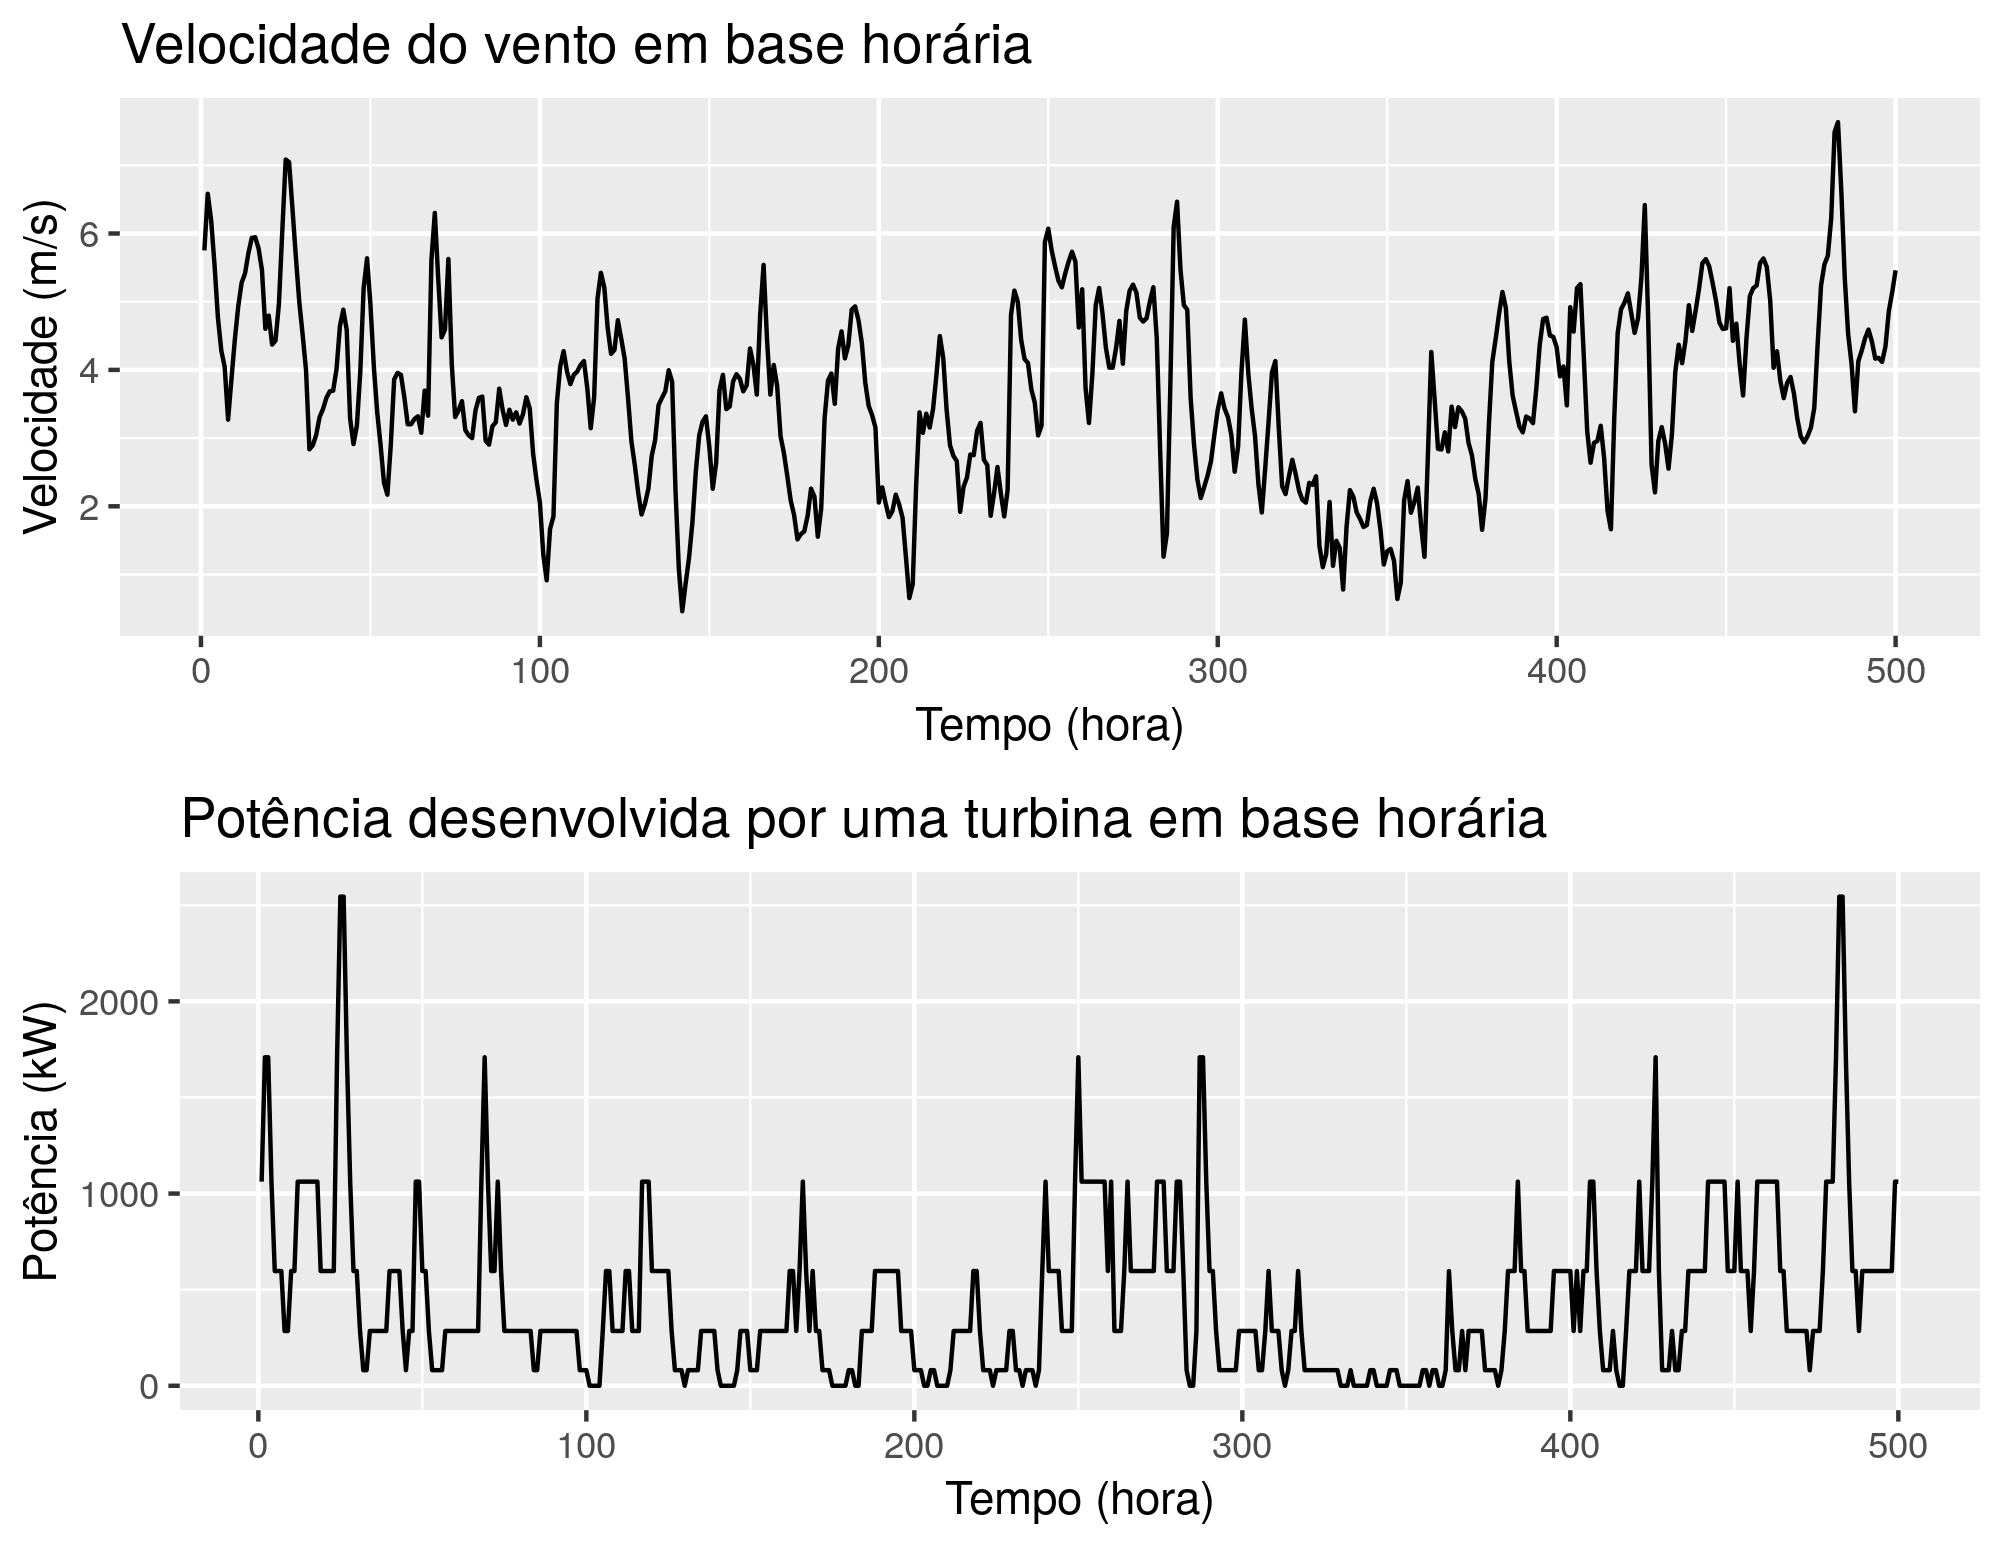
\includegraphics[width=\textwidth]{speed_power}
	\caption{Curva de potência de um aerogerador genérico.}
\end{figure}
\FloatBarrier

De acordo com essa curva a energia total produzida nas 500 horas previstas seria de 217 MWh. Embora durante o período considerado a geração tenha ficado distante da potência máxima, o aerogerador produziu uma quantidade expressiva de energia. Se no mesmo período de 500 horas o aerogerador operasse no seu valor máximo de 4.5 MW, seriam produzidos 2250 MWh. Para esse período o fator de capacidade foi baixo, apenas cerca de 0.1. É comum encontrar fatores entre 0.3 e 0.5 em parques operacionais no país. É interessante perceber que caso o proprietário do parque fechasse um acordo de produção de energia considerando um fator de capacidade relativamente pessimista de 0.3 (o limite inferior da média dos parques do país) ele perderia dinheiro pois durante o período o fator de capacidade ficou abaixo de 0.1.

\chapter{Validação com outras séries}

O modelo que obteve o melhor poder preditivo foi o GARCH(1,1). No entanto, assim como todos os outros modelos discutidos, os testes  de poder preditivo foram feitos apenas sob uma única série, aquela apresentada na seção \ref{modelo}. Há regiões em que a distribuição que melhor descreve o recurso eólico é  a de Weibull, em outras é a distribuição Rayleigh, beta, normal ou log-normal \cite{dists}. O vento pode ainda ser unidirecional, bidirecional ter mais de uma direção predominante. Como fora exposto, a série modelo é melhor descrita por uma distribuição beta (Figura ~\ref{fig:cullen}) e é predominantemente unidirecional (Figura ~\ref{fig:windrose}). Dessa forma é interessante validar o modelo aplicando-o em diversas outras séries correspondentes a diferentes regiões cujo recurso eólico seja distinto. 

62 regiões foram escolhidas. 7 na América Central, 1 no Jordão e as demais na América do Sul. A distribuição desigual se deve ao fato de que essas séries correspondem a estudos comerciais ao qual o autor tem acesso. Explica-se dessa forma o fato de a grande maioria das séries localizarem-se no Nordeste do Brasil. Todas as séries utilizadas, no entanto, são oriundas do banco de dados de acesso público ERA5 da ECWMF. Essas localidades são exibidas abaixo:

\begin{figure}[h]
    \centering
	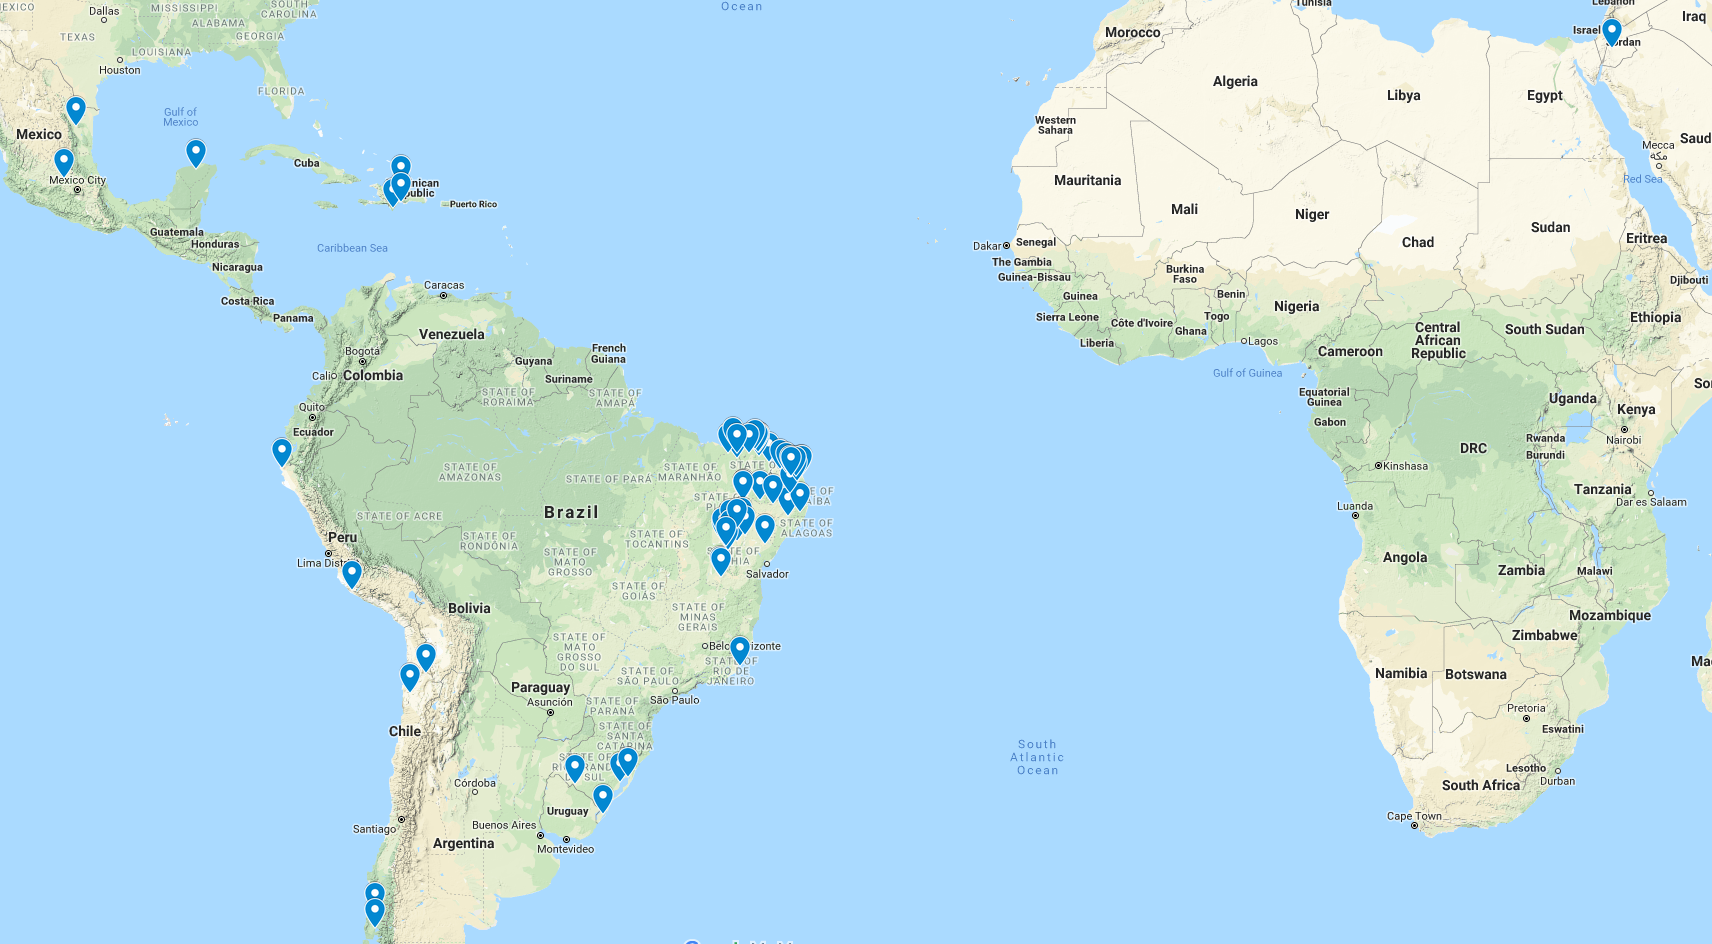
\includegraphics[width=\textwidth]{latam}
	\caption{Regiões correspondentes a dados de velocidade do vento do banco de dados ERA5 da ECWMF. Mapa disponível em }
\end{figure}
\FloatBarrier

As regiões escolhidas variam entre florestadas, desérticas, no interior de continentes ou diretamente na costa ou ainda em golfos ou ilhas. O sucesso do modelo em regiões tão distintas leva a crer que ela seja aplicável a condições bem gerais.

O modelo GARCH(1,1) foi aplicado em cada uma das séries cujas localidades correspondentes são exibidas no mapa acima e os resultados são exibidos abaixo:

\begin{table}[h]
\centering
\begin{tabular}{ |c|c|c|c|c|c| } 
\hline
\textbf{Local}&\textbf{ME}&\textbf{RMSE}&\textbf{MAE}&\textbf{MPE}&\textbf{MAPE}\\
\hline
NE01a&0.0&0.02&0.01&-0.0&0.17\\
\hline
NE05&0.01&0.02&0.01&0.02&0.17\\
\hline
ChapadaAraripe&0.01&0.02&0.01&0.02&0.17\\
\hline
Embuaca&-0.01&0.02&0.02&-0.16&0.27\\
\hline
Santos&-0.01&0.02&0.02&-0.16&0.27\\
\hline
LaGuajira&0.03&0.04&0.04&0.25&0.27\\
\hline
AsaBranca&0.02&0.03&0.02&0.19&0.28\\
\hline
Omega&0.02&0.03&0.03&0.14&0.28\\
\hline
Icarai&-0.01&0.02&0.02&-0.19&0.29\\
\hline
EsquinaDoVento&0.03&0.04&0.03&0.25&0.4\\
\hline
\end{tabular}
\caption{10 melhores localidades em relação a previsão com GARCH(1,1)}
\end{table}

\begin{table}[h]
\centering
\begin{tabular}{ |c|c|c|c|c|c| } 
\hline
\textbf{Local}&\textbf{ME}&\textbf{RMSE}&\textbf{MAE}&\textbf{MPE}&\textbf{MAPE}\\
\hline
Omega\_RJ&0.1&0.13&0.11&1.48&2.02\\
\hline
Ibipeba&-0.04&0.07&0.05&-1.83&2.11\\
\hline
Tafila\_ERA5&0.05&0.11&0.08&-0.19&2.33\\
\hline
CapaoAlto&0.0&0.07&0.06&-1.63&2.41\\
\hline
Quadran&-0.05&0.07&0.05&-2.48&2.61\\
\hline
LaVigia&-0.01&0.06&0.05&-2.28&3.12\\
\hline
Ckani&0.05&0.13&0.09&-0.95&3.35\\
\hline
SanPedro&0.08&0.17&0.12&-0.1&3.94\\
\hline
Tucano&-0.05&0.15&0.13&-3.74&4.8\\
\hline
Llanos&0.22&0.33&0.24&3.47&12.58\\
\hline
\end{tabular}
\caption{10 piores localidades em relação a previsão com GARCH(1,1)}
\end{table}





































%\cleardoublepage
%\part{Análise de dados de vento}
%
%\chapter{Características de longo prazo}
%
%É interessante exemplificar as discussões subsequentes com dados reais de medição. O Centro Europeu de Previsões Metereológicas de Médio Prazo (ECMWF, sigla em inglês) disponibiliza publicamente dados metereológicos de todo o globo medidos por satélite, incluindo dados de velocidade e direção do vento compilados no banco de dados ERA5 \cite{era5}. Os dados de velocidade do vento são referentes a uma altura de 80 metros e possuem resolução de 30 quilômetros. As unidades de todas as grandezas referenciadas neste trabalho seguem o padrão SI. Em particular velocidade é dada em metros por segundo e o tempo em segundos. A partir de uma posição do globo dada em latitude e longitude como entrada obtém-se da ECMWF uma série temporal com 18 variáveis: 9 de velocidade do vento e 9 de direção referentes aos nove quadrantes que circundam a posição informada: quadrante central, norte, sul, sudeste, etc. 
%
%A figura abaixo mostra esses quadrantes para uma região no norte baiano, na cidade de Sento Sé para a posição 9.8436 S, 41.1912 W.
%
%\begin{figure}[h]
%    \centering
%%	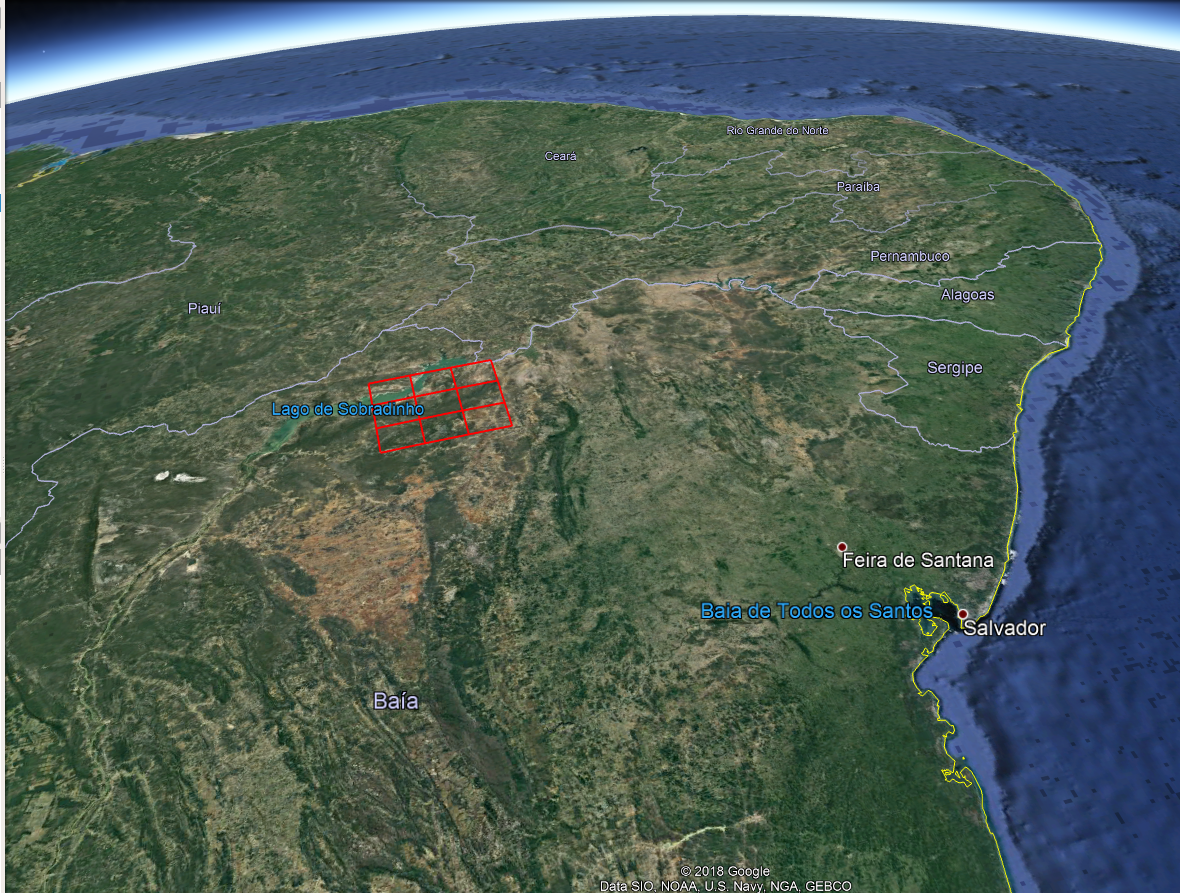
\includegraphics[scale=0.5]{earth}
%	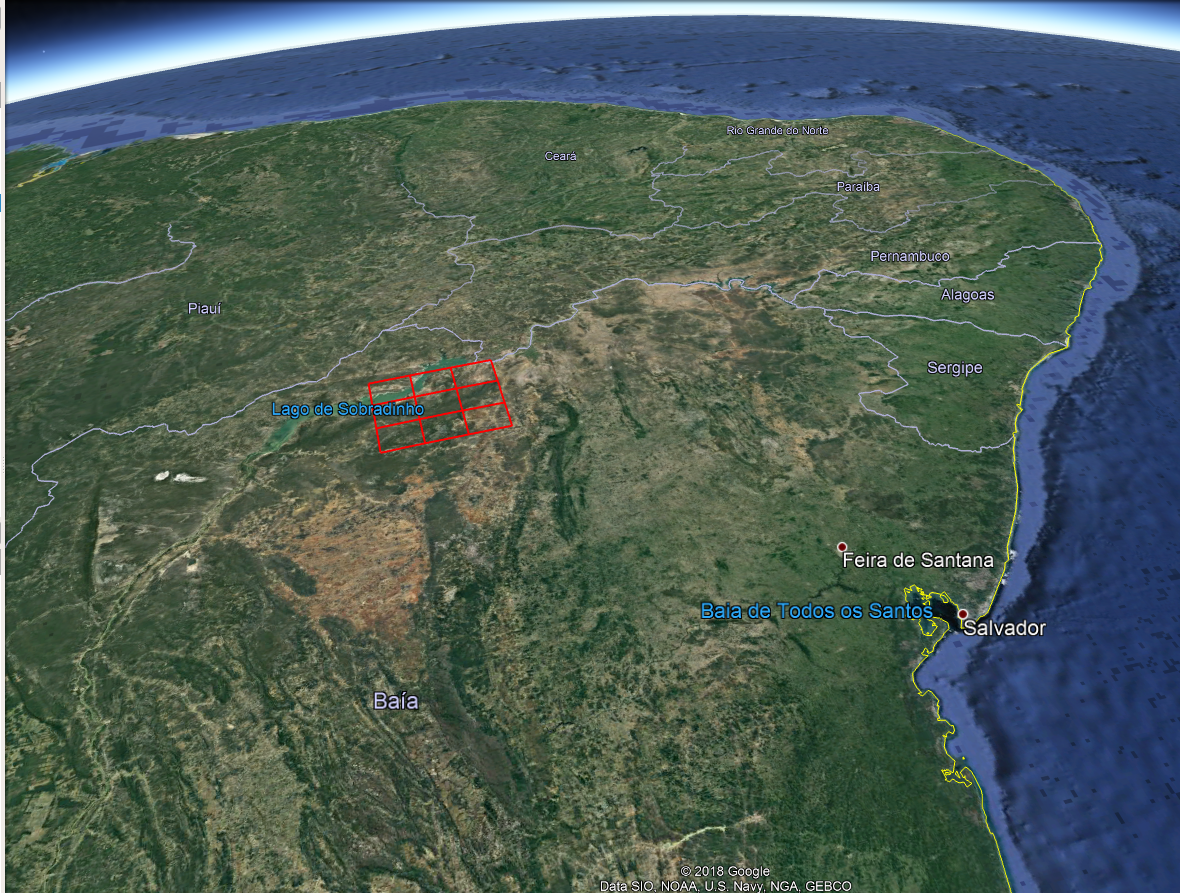
\includegraphics[scale=0.6]{earth}
%	\caption{Localização da região de medição por satélite dos dados de vento discutidos no texto. Fonte: SIO, NOAA, U.S. Navy, NGA, GEBCO. \textcopyright \  2018 Google}
%\end{figure}
%\FloatBarrier
%
%A partir de análises de diversas localidades do Nordeste brasileiro sabe-se que o recurso eólico dessa região é representativo de todo o Nordeste do país, isto é, a velocidade média do vento é alta, predominantemente entre 6 e 8 m/s, fortemente unidirecional a jusante de sudeste a 120º em relação ao norte geográfico, com uma componente significativamente menor, mas relevante, a cerca de 150º como pode ser observado na rosa dos ventos gerada a partir dos dados medidos para o ano de 2017:
%
%\begin{figure}[h]
%    \centering
%	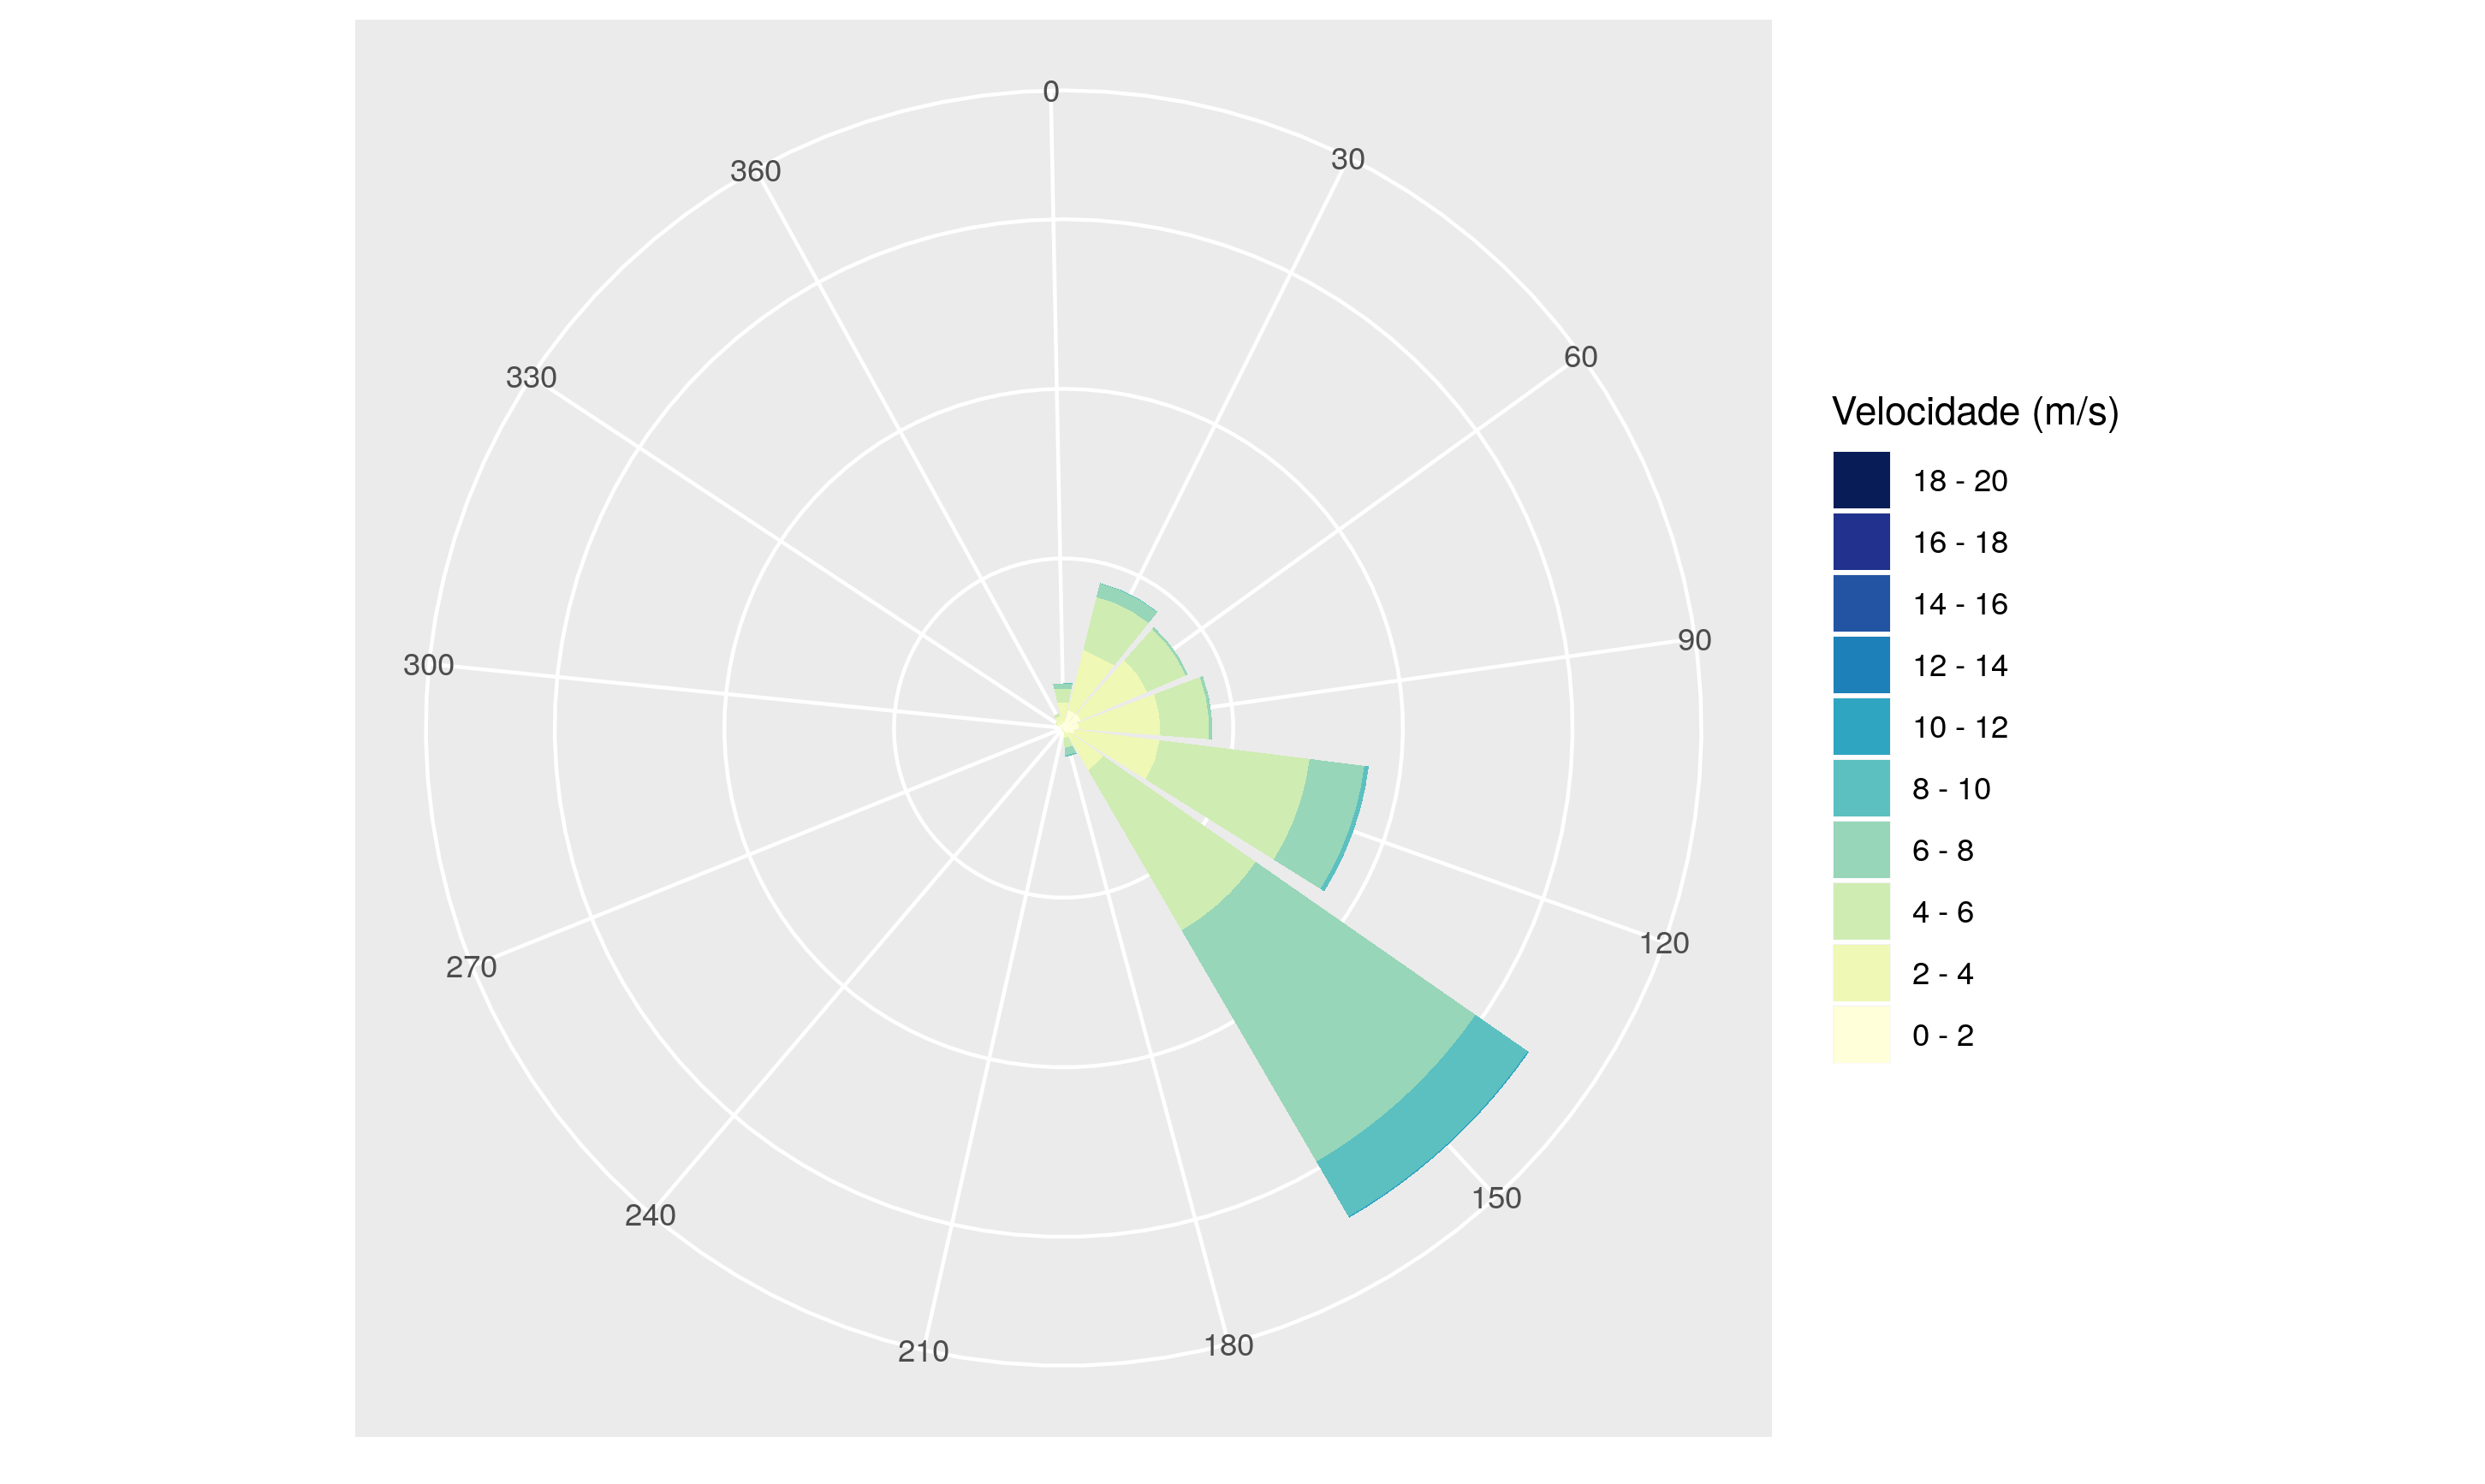
\includegraphics[scale=0.9]{windrose}
%	\caption{Rosa dos ventos do recurso eólico da cidade de Sento Sé no norte da Bahia - característico do Nordeste brasileiro,  a partir de dados medidos para o ano de 2017. Fonte: autoria própria, dados \cite{era5}.}
%\end{figure}
%\FloatBarrier
%
%\newpage
%Analisando as rosas dos ventos mensais se confirma o comportamento anual e também é possível observar que nos meses de junho a outubro a velocidade do vento é muito alta enquanto que nos demais meses, de Novembro a Maio, ela é muito menor. Com essa informação, é possível, por exemplo, nos meses de baixa velocidade e consequente baixa geração de energia, complementar o suprimento energético do local com outras fontes de energia renovável tal como a energia solar que apresenta o comportamento inverso à energia eólica na região, isto é, nos meses de primavera e verão a elevada altitude solar permite extrair a maior proporção de energia anual ao contrário dos meses de outono e inverno.
%
%\begin{figure}[h]
%    \centering
%  	\hspace*{-1.4cm}   
%	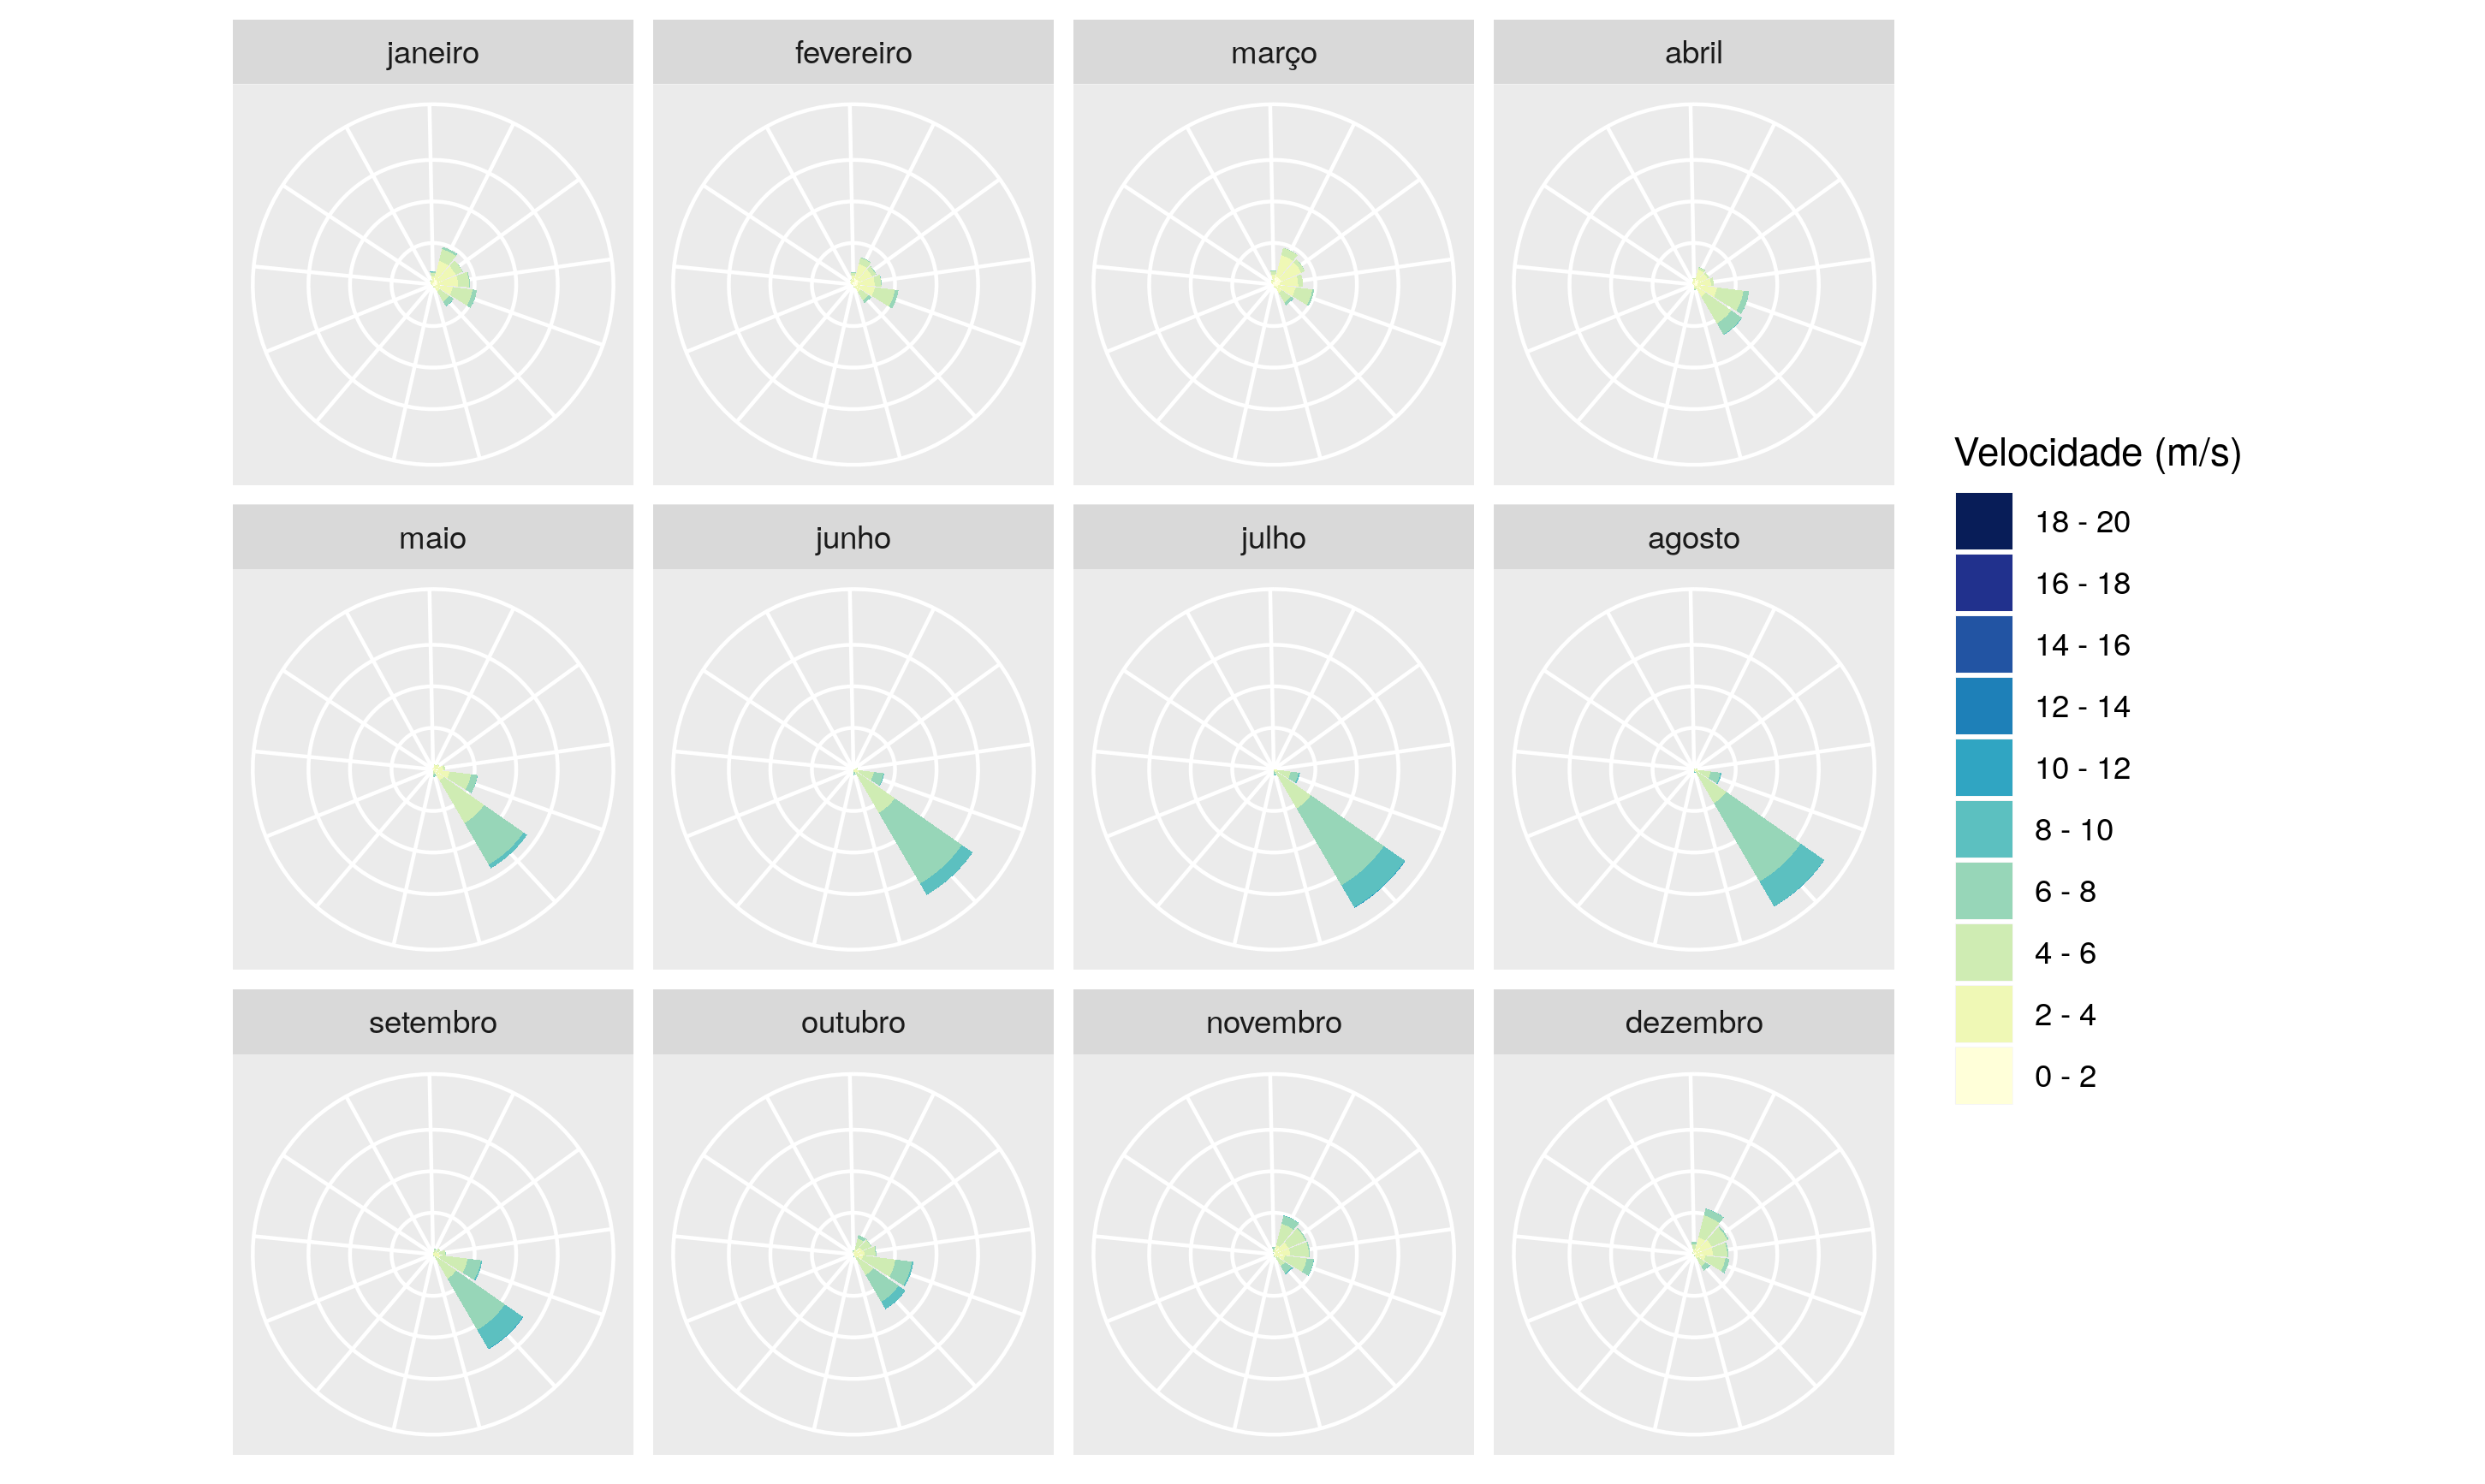
\includegraphics[scale=1]{windrose_monthly}
%	\caption{Rosas dos ventos mensais do recurso eólico da cidade de Sento Sé no norte da Bahia a partir de dados medidos para o ano de 2017. Fonte: autoria própria, dados \cite{era5}.}
%\end{figure}
%\FloatBarrier
%
%\chapter{Características de curto prazo}
%
%Sabe-se que em períodos curtos, o vento apresenta um comportamento que aparenta ser puramente estocástico, associado ao comportamento turbulento característico da dinâmica de fluídos pouco viscosos tal como o ar. No entanto, observando períodos maiores de tempo, tais como dias, meses e anos observa-se que existem tendências coexistentes com o caráter aleatório, errático do vento. É tarefa da ciência de dados evidenciar a presença desses padrões a partir dos dados medidos, pois, apenas exibindo graficamente a evolução temporal da velocidade do vento leva a crer que não exista qualquer tendência ou padrão nestes dados:
%
%\begin{figure}[h]
%    \centering
%	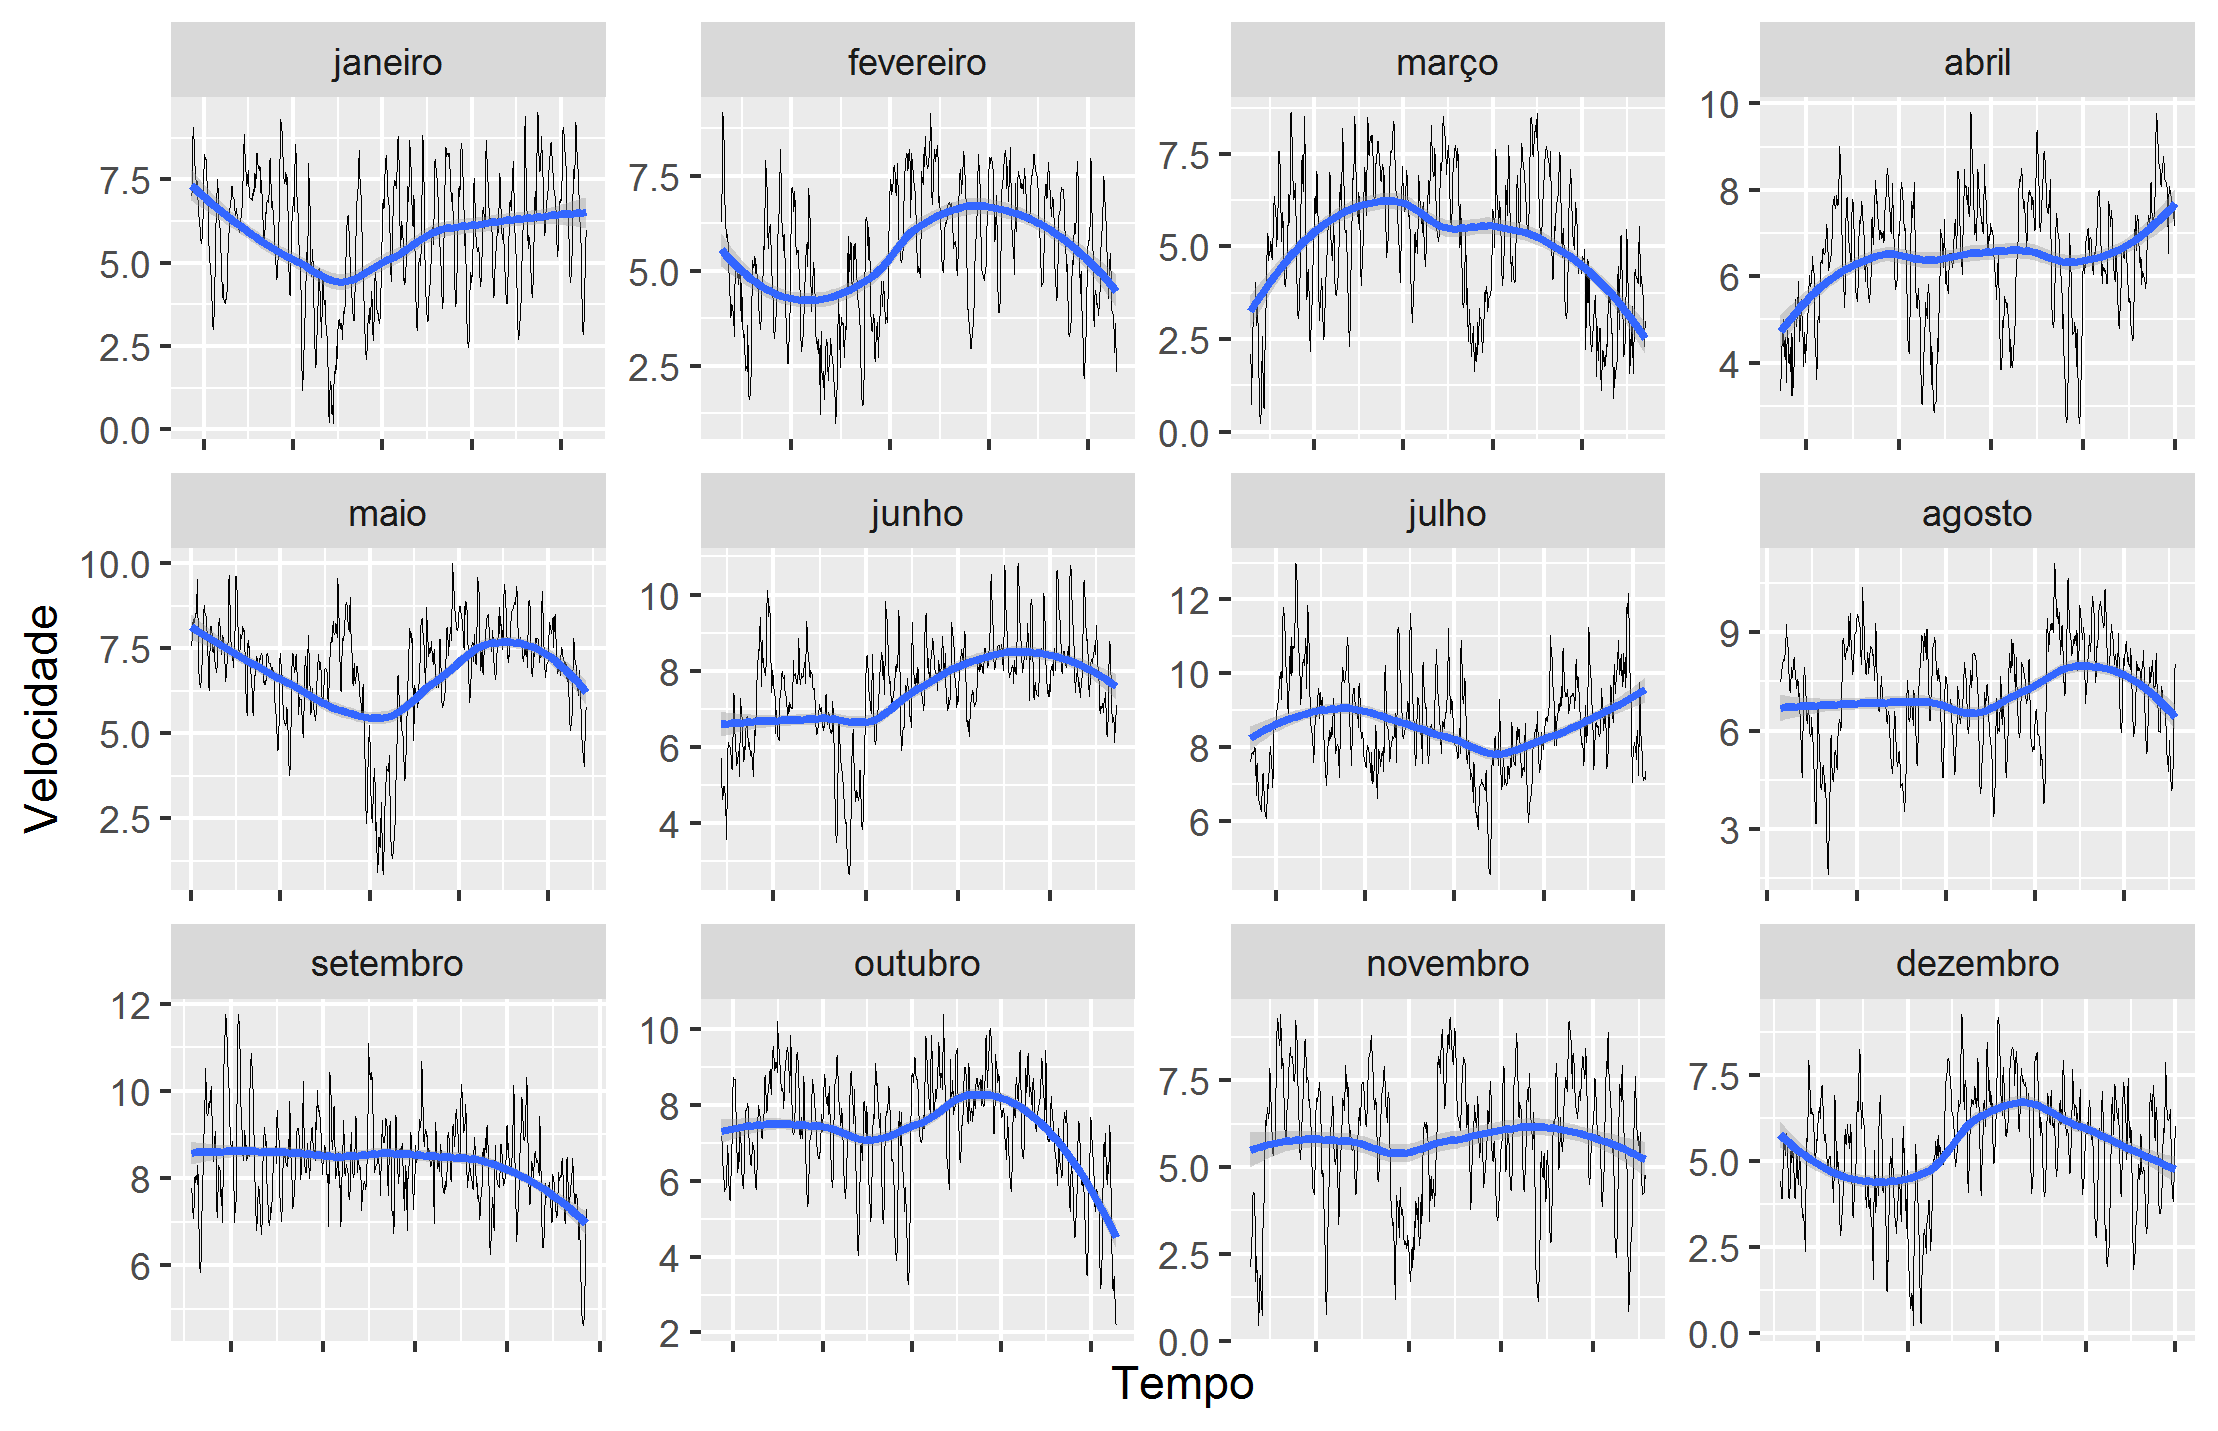
\includegraphics[scale=0.85]{stochastic_monthly}
%	\caption{Velocidade do vento para cada mês do ano de 2017 da cidade de Sento Sé no norte da Bahia. Curva em preto: dados medidos. Curva em azul: curva ajustada aos dados medidos. Fonte: autoria própria, dados \cite{era5}.}
%\end{figure}
%\FloatBarrier
%
%A figura abaixo apresenta a variação horária da velocidade do vento para cada mês do ano para a cidade de Sento Sé.
%Observa-se que o vento no local apresenta um ciclo diário característico e que está presente em todos os meses do ano. De acordo com \cite{art10} o ciclo diário do vento é um fator mais relevante do que a velocidade média do vento para definir a localização de um parque eólico, devido a relação entre a geração horária de energia e a demanda correspondente. Embora a velocidade do vento seja bem mais alta em Julho do que em Janeiro, em ambos os meses tem-se um mínimo de velocidade durante o meio da tarde, uma taxa de variação positiva a medida que a noite se aproxima e uma estabilização durante a madrugada e primeiras horas da manhã. O mesmo vale para os demais meses.
%Pode-se explicar esse fenômeno observado que durante o dia o aquecimento da atmosfera pelo Sol torna o vento turbulento sendo mais difícil o seu aproveitamento para geração de energia, pois sua velocidade direcional é baixa. À noite, por outro lado, a atmosfera se estratifica, o vento fica pouco turbulento e a sua velocidade direcional aumenta. Essa explicação embora válida para este local pode não ser para outro, pois existem diversos fatores, além do aquecimento local da atmosfera, que definem o comportamento do vento. Em regiões desérticas, por exemplo, observa-se uma alta estabilidade na atmosfera devido à baixa umidade. A mesma explicação pode ser estendida para descrever o comportamento mensal: durante meses de inverno e outono a velocidade do vento é alta, enquanto que em meses de verão e primavera ela é baixa. 
%
%\begin{figure}[h]
%    \centering
%	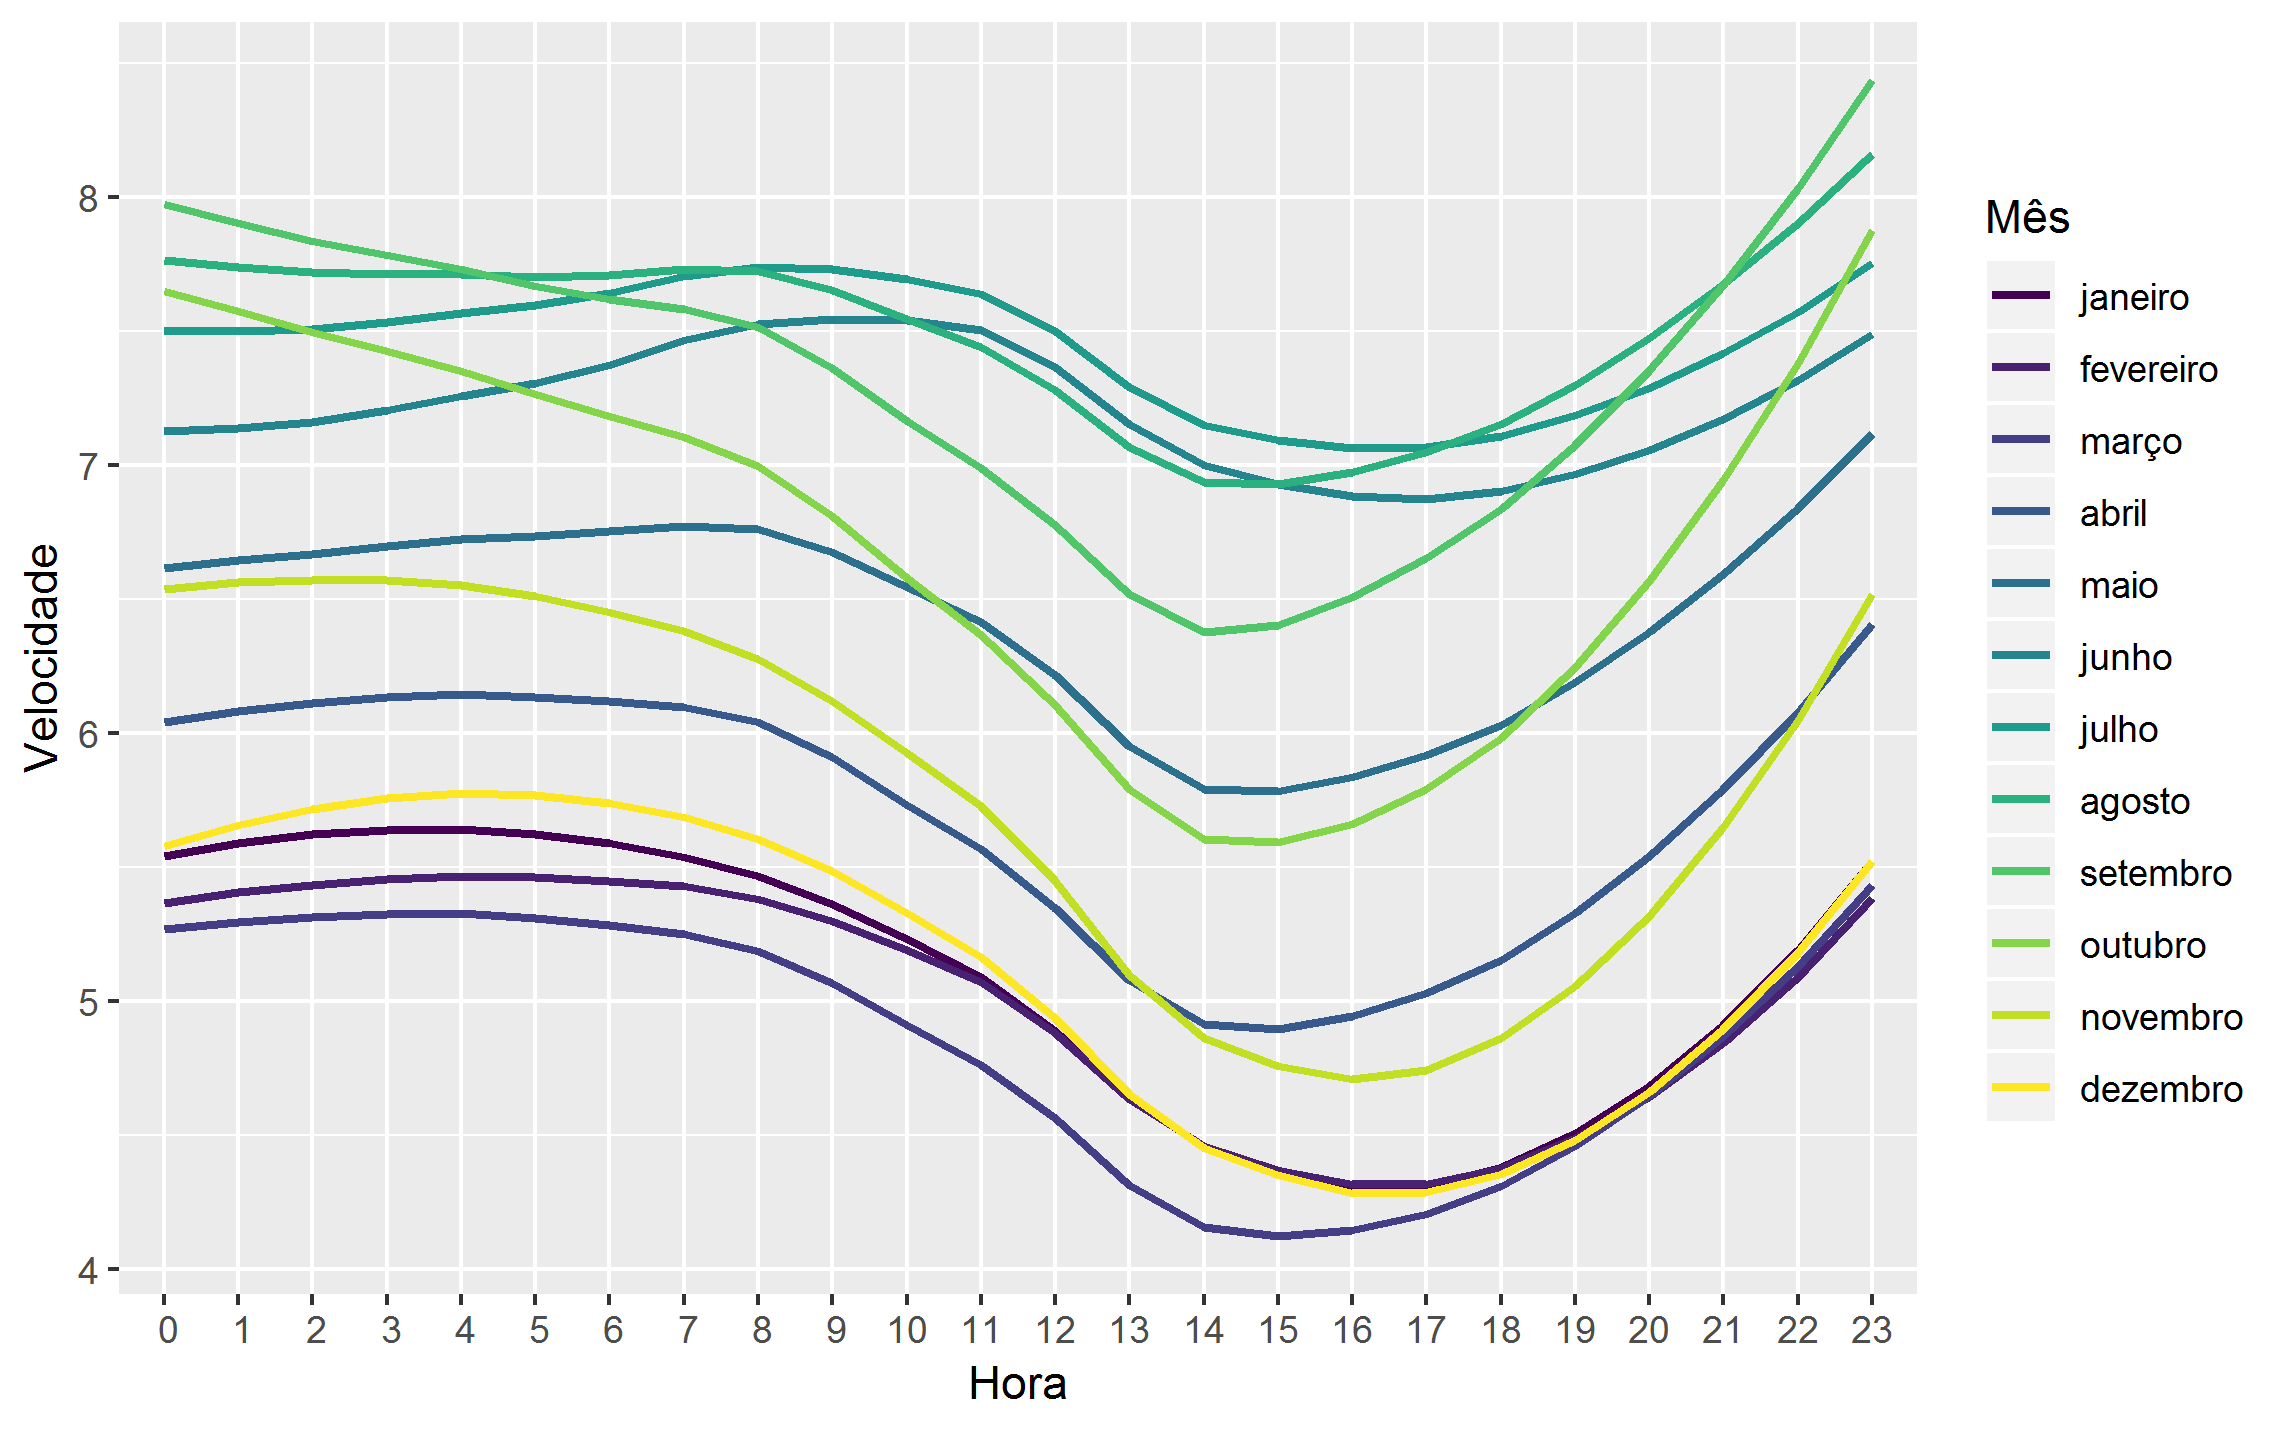
\includegraphics[width=\textwidth]{diurnal}
%	\caption{Velocidade do vento para cada hora do dia e para cada mês do ano de 2017 para a cidade de Sento Sé no norte da Bahia. Fonte: autoria própria, dados \cite{era5}.}
%\end{figure}
%\FloatBarrier
%
%\part{Embasamento teórico}
%
%\chapter{Embasamento matemático}
%
%A separação entre o que é fundamentalmente aleatório e o que exibe uma tendência em alguma janela temporal é de extrema relevância para a concepção de um modelo matemático que descreva tal fenômeno. Essas contribuições podem ter origens físicas diferentes e a formulação das equações diferenciais estocásticas envolve a distinção entre um termo associado à deriva e outro à difusão o qual não contribui para o valor esperado da variável em questão, isto é, na ausência de deriva, o valor esperado da variável estocástica seria zero, em outras palavras, ele distribui a variância igualmente para mais e para menos.
%
%Um processo estocástico contínuo no tempo, $ W(t) $, definido para $ t>=0 $ com $W(0)=0$ tal que o incremento $ W(t)-W(s)$ é dado por uma distribuição gaussiana com média $0$ e variância $t-s$ para qualquer $ 0<=s<t$ sendo tais incrementos, restritos aos que não se sobrepõem no tempo, independentes, recebe o nome de processo de Wiener \cite{wiener}. O movimento browniano é um exemplo particular de processo de Wiener.
%
%O processo $S_t$ descrito pela equação estocástica abaixo, por exemplo \cite{art27}, possui o termo de deriva $\mu S_t dt$ e o termo de difusão dado por $\sigma S_t dW_t$ o qual está associado a um processo de Wiener representado por $W_t$:
%
%\begin{equation}
%dS_t = \mu(S_t,t) dt + \sigma(S_t,t) dW_t
%\end{equation}
%
%
%Um processo estocástico cujo valor esperado futuro é igual ao valor presente é classificado como um \textit{martingale} \cite{stevens}. Essa é uma característica importante da análise, pois diversos teoremas a tem como hipótese. É claro que a teoria encontraria pouca aplicação prática se não contemplasse processos que envolvem deriva. Para tanto, o teorema de Girsanov \cite{stevens} garante que tal processo, sujeito a algumas hipóteses pouco restritivas, pode tornar-se um \textit{martingale} por meio de uma mudança de escala - uma função multiplicativa apropriada a qual é conhecida como derivada de Radon-Nikodym \cite{stevens}.
%
%\newpage
%A evolução histórica do preço das ações da Google na NASDAQ bolsa, por exemplo, apesar de ter caráter estocástico, apresenta claramente uma tendência de subida (uma deriva, ou \textit{drift} do inglês):
%
%\begin{figure}[h]
%    \centering
%	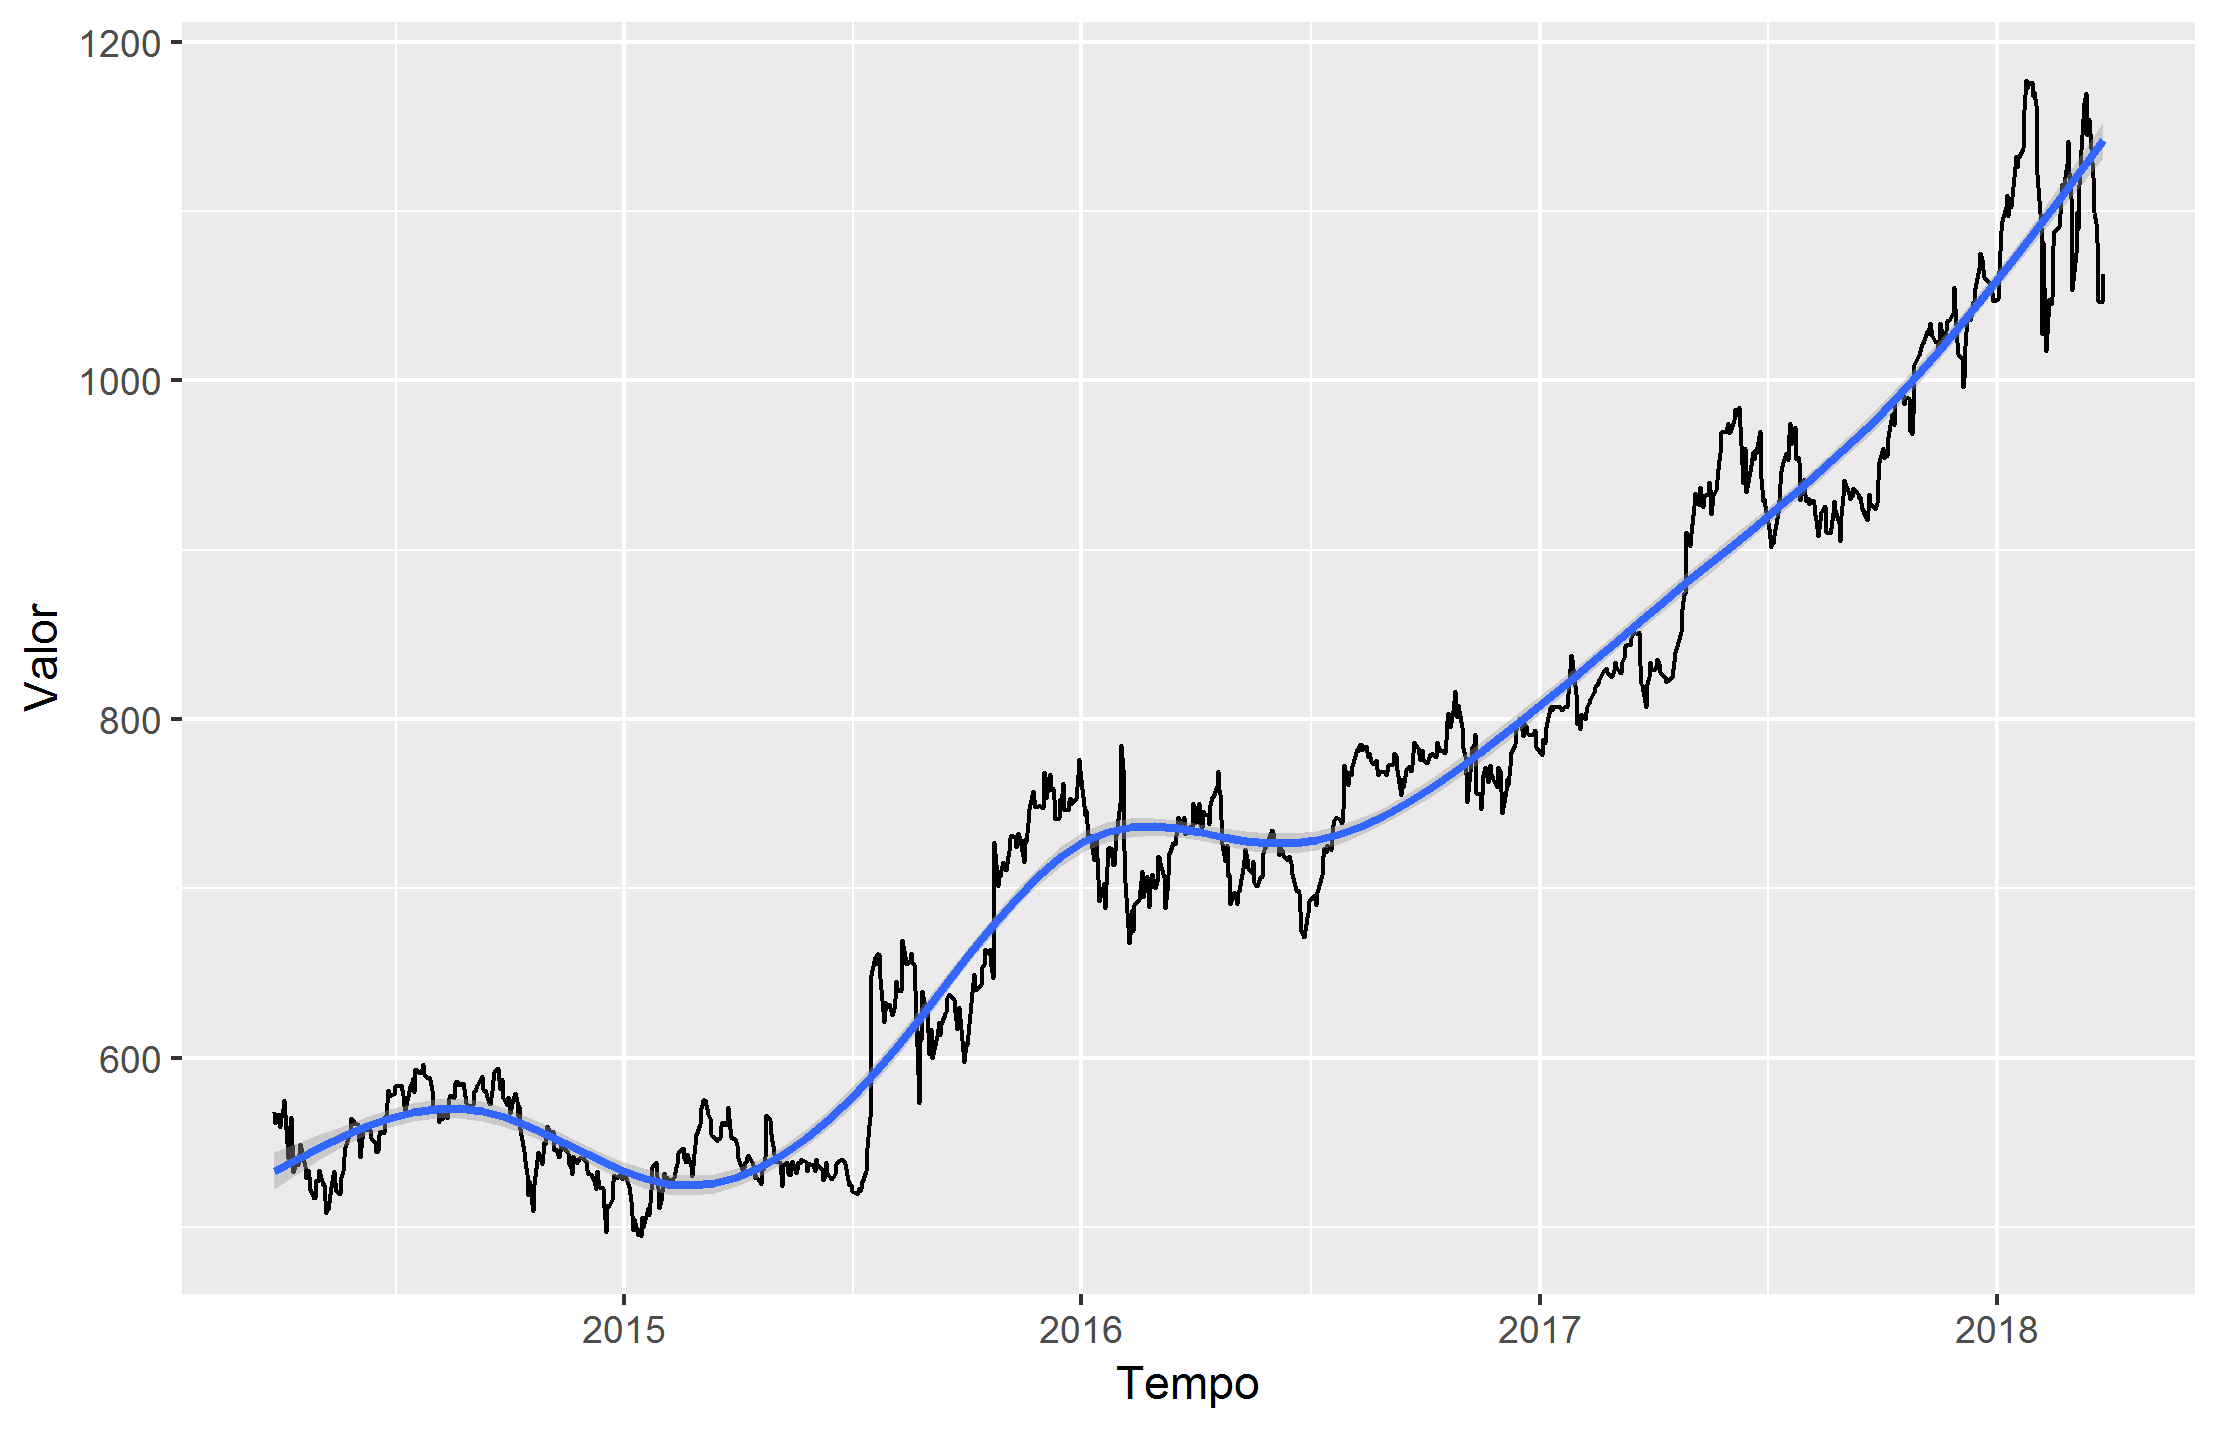
\includegraphics[width=\textwidth]{stock}
%	\caption{Valor de abertura das ações da Google na NASDAQ. Curva em preto: dados medidos. Curva em azul: curva ajustada aos dados medidos. Fonte: autoria própria, dados \cite{nasdaq}.}
%\end{figure}
%\FloatBarrier
%
%%orografia, rugosidade
%%Cada local tem suas muitas características específicas (orografia, rugosidade, posição no globo, entre outras) e qualquer padrão observado para um local pode não apenas não ser válido para outro local mas pode ocorrer o fenômeno oposto.
%
%%coleta de dados de vento: botar umas torres
%
%\chapter{Embasamento físico}
%
%%João e Paulo não gostam de Juriscleide. Este (latter) a acha fedida, aquele (former), desbocada.
%
%\section{Restrições físicas}
%Como fora exposto, a velocidade do vento apresenta várias tendências de longo prazo, comportamentos periódicos - sazonais e até horários e padrões característicos de orografia, clima e latitude. No entanto, essa é uma grandeza fundamentalmente estocástica, isto é, está associada a uma variável aleatória e portanto, a sua previsão está fadada a uma incerteza intrínseca. Antes da formulação da mecânica quântica acreditava-se que se conhecendo perfeitamente o Hamiltoniano de um sistema, isto é, sabendo a posição e momento de todas as partículas que o compõe, seria possível prever com exatidão a sua evolução temporal, ao menos em tese (dado que tal feito é inviável para qualquer sistema moderamente complexo). No entanto, o princípio da incerteza de Heisenberg pôs fim a essa crença, visto que enuncia que não somente é impossível saber simultaneamente a posição e momento exatos de uma particula como não faz sentido falar da simultaneidade das duas grandezas; tampouco é útil a informação sobre velocidade e momento de todas as partículas de um sistema, pois as grandezas de interesse são de natureza estatística, como a temperatura por exemplo. 
%
%A mecânica estatística desenvolveu-se em paralelo ignorando a busca pela determinação exata da evolução temporal de um sistema. Ao invés disso, concentrou-se em determinar valores médios de quantidades de interesse emergentes do comportamento caótico fundamentada na hipótese de que todas as possíveis configurações do sistema ocorrem com igual probabilidade. Apesar do grande sucesso em diversas áreas da física foi incapaz de explicar o comportamento turbulento de fluídos, foi incapaz de explicar como que surge ordem a partir do caos. Relativamente pouco progresso foi feito até então \cite{chaos}. É por esse motivo que frequentemente a previsão do tempo falha, até mesmo em uma escala de horas independente de quantas estações metereológicas sejam utilizadas, já que de acordo com a teoria do caos existe um horizonte de previsão \cite{ian} a partir do qual não é possível obter estimativas confiáveis. A teoria do caos mostrou que a ignorância quanto a natureza da complexidade era muito maior. Tome como exemplo um sistema simples com uma variável discreta $x_t$ e uma regra de evolução temporal não-linear, $x_{t+1}=x_t(1+x_t)$ \cite{NOSRATI2018224}. Conhece-se tudo sobre esse sistema. Ele é perfeitamente determinístico. Ainda assim existe um certo instante de tempo a partir do qual não é possível predizer o seu estado futuro. Esse instante chama-se de transição ao caos \cite{lorenz}.
%
%\section{Abordagem de longo prazo}
%
%Fênomenos fortemente não-lineares como a turbulência, não são, no entanto, completamente imprevisíveis. Acredita-se que dependendo do sistema e sujeito às restrições expostas acima a tarefa seja factível, porém não existe uma única maneira de abordar tal problema. Este trabalho propõe a investigação de qual modelo produz melhores resultados de estimativa de produção de energia, começando por um modelo de evolução temporal de velocidade do vento que faça uso dos dados de medição para encontrar a distribuição de probabilidade associada à essa grandeza.
%
%É prática comum na indústria a determinação da distribuição de probabilidade de energia a partir de simulações de Monte Carlo \cite{portacopos} tendo como hipótese que a velocidade do vento é descrita por uma distribuição de Weibull a qual já foi verificada experimentalmente a partir de muitas análises de dados de vento e tem sólido embasamento teórico conforme o teorema de Fisher–Tippett–Gnedenko, o qual prova que o máximo de um conjunto de variáveis aleatórias independentes, após renormalização, converge apenas para uma de três classes de distribuições: a distribuição de Gumbel, a distribuição de Fréchet ou a distribuição de Weibull \cite{fisher}.
%
%Para a cidade de Sento Sé, por exemplo, a distribuição de velocidades do quadrante central é exibida abaixo:
%
%\begin{figure}[h]
%    \centering
%	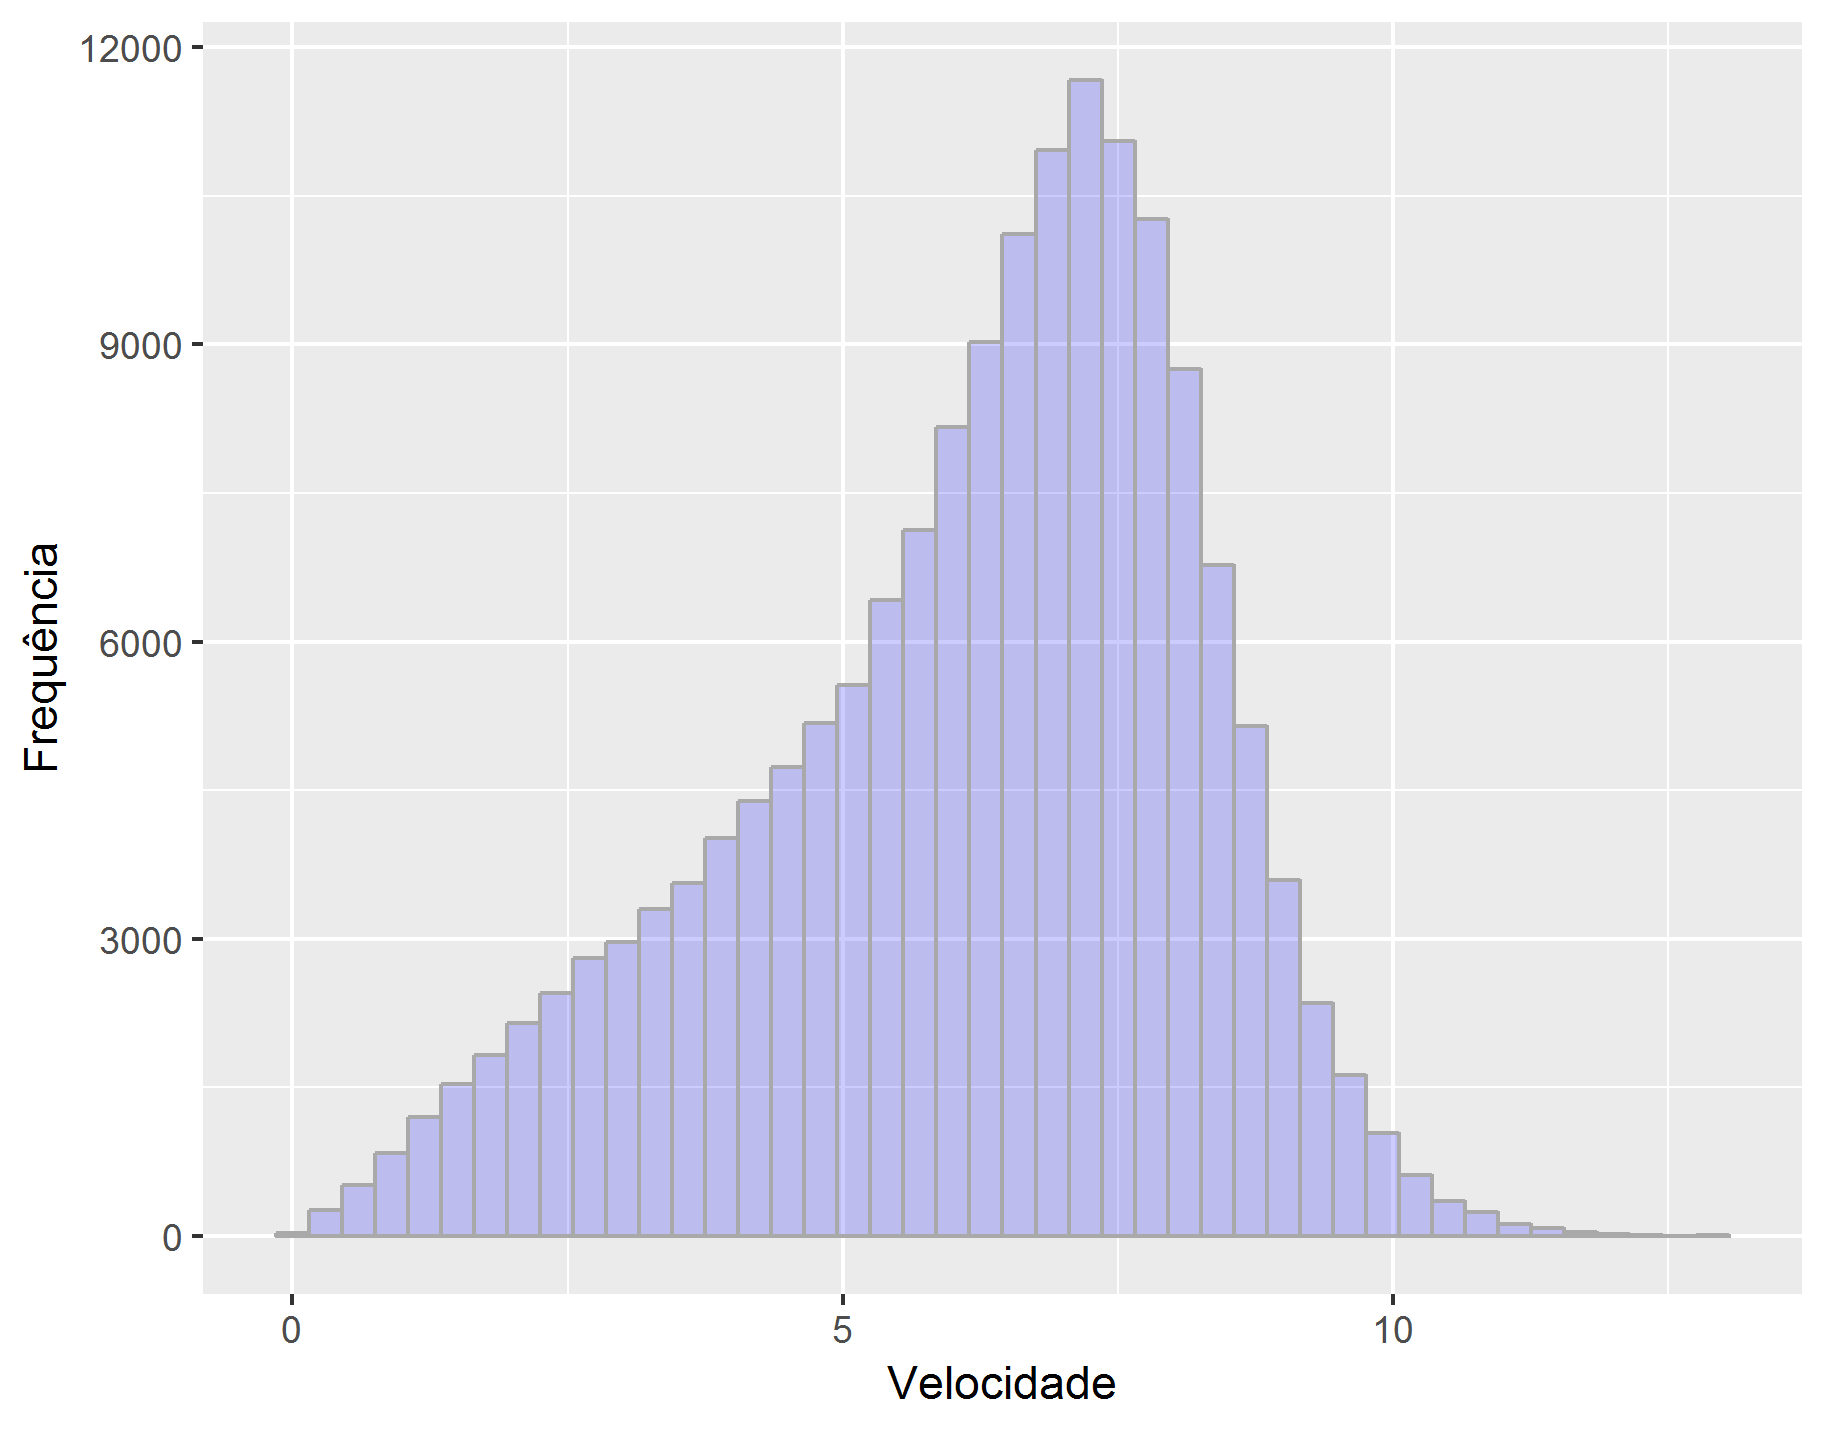
\includegraphics[scale=0.8]{weibull_histogram}
%	\caption{A distribuição de velocidades pode ser aproximada por uma distribuição de Weibull. Dados do quadrante central dos dados ERA5 \cite{era5} para a cidade de Sento Sé no norte da Bahia. Fonte: autoria própria, dados \cite{era5}.}
%\end{figure}
%\FloatBarrier
%
%Essa distribuição claramente não é gaussiana porque possui uma cauda unilateral. Tal distribuição é representada satisfatoriamente por uma distribuição de Weibull por meio de dois parâmetros: o parâmetro de forma $k$ e o parâmetro de escala $\lambda$. Seus primeiros momentos são definidos por \cite{weibull}:
%
%\begin{equation}
%	\left<v\right> = \lambda\Gamma\left(1+\frac{1}{k}\right)
%\end{equation}
%
%\begin{equation}
%	\sigma^2 = \lambda^2\left\{\Gamma\left(1+\frac{2}{k}\right)-\left[\Gamma\left(1+\frac{1}{k}\right)\right]^2\right\}
%\end{equation}
%
%Avaliando a distribuição de densidade de probabilidade de velocidade para todos os quadrantes dos dados de vento da cidade de Sento Sé, confirma-se que todos seguem uma distribuição do tipo weibull. Sabendo que a direção preferencial do vento é sul-sudeste observa-se, a partir das curvas para norte, nordeste e noroeste, que à medida que flui no local a velocidade média aumenta.
%
%\begin{figure}[h]
%    \centering
%	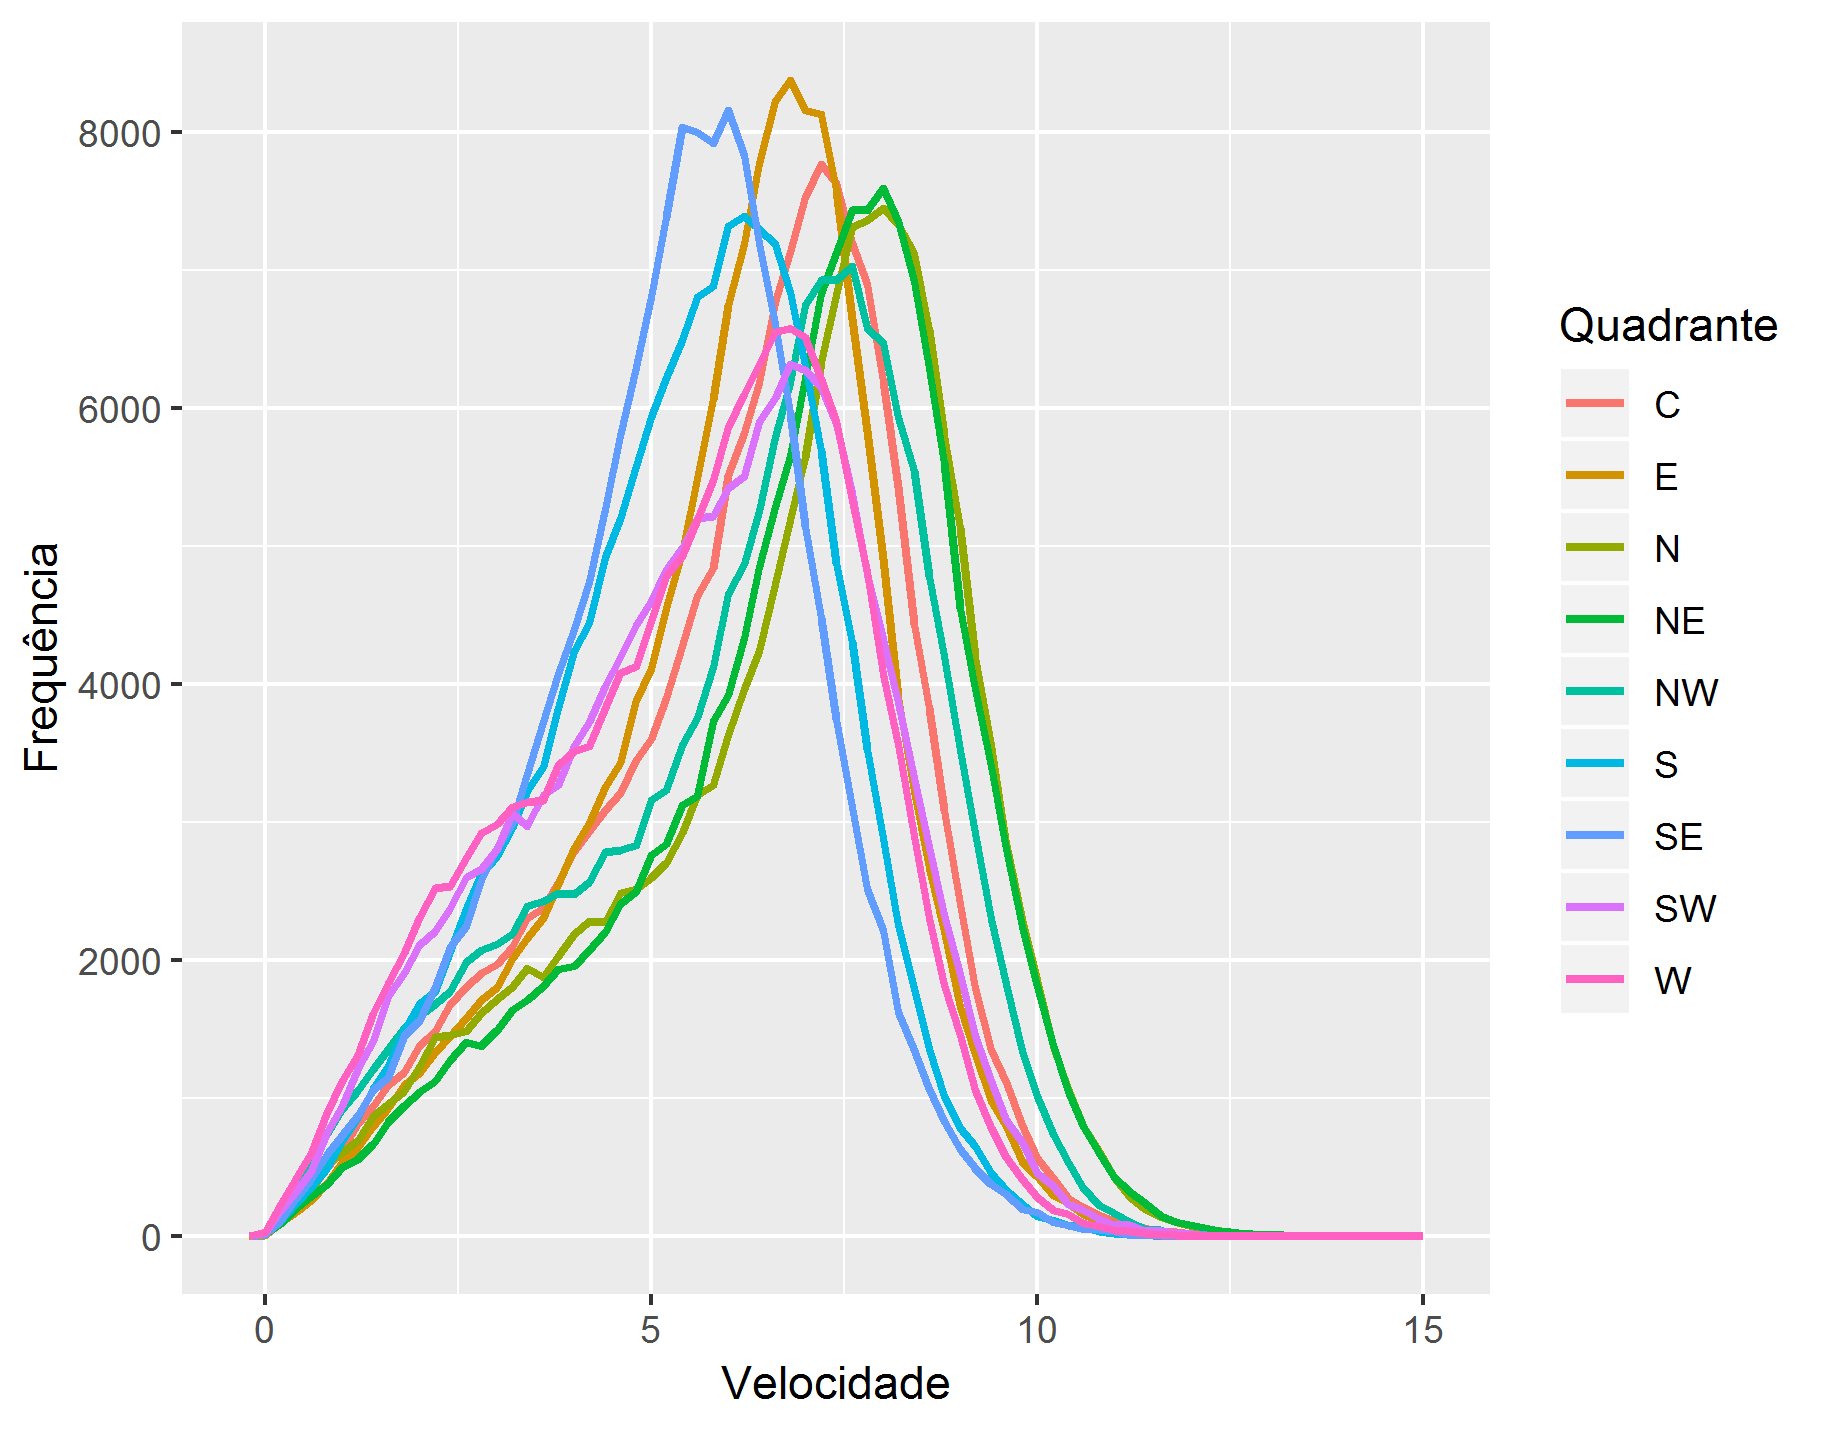
\includegraphics[scale=0.85]{weibull_freqpoly}
%	\caption{Distribuição de velocidades de todos os quadrantes dos dados ERA5 \cite{era5} para a cidade de Sento Sé no norte da Bahia. Fonte: autoria própria, dados \cite{era5}.}
%\end{figure}
%\FloatBarrier
%
%Os parâmetros $\lambda$ e $k$ são utilizados para caracterizar o recurso eólico em uma dada posição (latitude e longitude) e altura. Para obter o recurso eólico em outra posição ou altura (posição e altura de uma turbina por exemplo) é feito um escalonamento da distribuição: muda-se a sua forma para obter um valor esperado de velocidade correspondente à nova posição.
%
%\section{Desvantagens}
%
%Essa abordagem embora adequada para estimativas de longo prazo e muito utilizada na indústria possui várias desvantagens:
%
%\begin{itemize}
%    \item A hipótese da distribuição de Weibull é completamente inválida a curto prazo, visto que é uma distribuição constante e não pode, portanto, representar as flutuações incessantes características do comportamento turbulento do vento \cite{artmain}. Uma distribuição de probabilidade que descreva adequadamente a velocidade do vento deve ser dependente do tempo. A evolução temporal horária ou até mesmo minuto a minuto é uma informação essencial para operadores de subestações de distribuição de energia elétrica, pois permite adequar oferta de energia a picos e baixas de demanda os quais são conhecidos    
%    \item A simulação é lenta. O Método de Monte Carlo, como aplicado pela indústria, é um método de força bruta, ou seja, lança mão de poder computacional para atingir seu objetivo. E deve ser realizado toda a vez que se deseje obter o mesmo resultado ao passo que um modelo físico permite que o esforço computacional seja empregado apenas uma vez e, além disso, exige menos poder computacional. É impensável refazer tais cálculos a cada hora.
%    \item O método de Monte Carlo, como aplicado nessa problema, é apenas um recurso computacional, não descreve o comportamento físico do sistema e portanto não pode ser empregado em análises sofisticadas tais como mensurar a dependência temporal e espacial entre dois parques eólicos, ou seja, mensurar o efeito de esteira \cite{atlas} em resolução horária, podendo, por exemplo, como resultado conceber uma estratégia de gerenciamente setorial conjunto entre os dois parques, ou seja, orientar as turbinas dos dois parques de maneira mutuamente benéfica. Outro exemplo, seria prever o melhor intervalo de tempo para realizar a manutenção de uma turbina levando em conta o tempo necessário para realizar a manutenção as quais são, via de regra, custosas e demoradas.
%\end{itemize}
%
%\section{Ressalvas}
%
%Existem muitas fontes de incerteza ao longo de todo o processo de estimativa da produção de energia. Incerteza na obtenção dos dados de medição, na conversão entre velocidade e energia, na extrapolação horizontal (do local de medição à posição das turbinas), da extrapolação vertical (da altura da medição à altura das turbinas) entre muitas outras. A consideração dessas fontes de incerteza fogem ao escopo do presente trabalho mas devem ser todas consideradas em qualquer trabalho comercial. Pode-se dizer que este trabalho estuda o caso particular em que a medição do vento é feita a alguns diâmetros de rotor de distância da turbina, exatamente na altura do cubo rotor.
%
%\part{Revisão bibliográfica}
%
%A área de estudo deste trabalho possui vasta literatura. Modelos autoregressivos de média móvel (ARMA) foram utilizados em \cite{art20} para prever tanto a velocidade quanto a direção do vento. 
%
%Uma revisão bibliográfica dos vários métodos de previsão de dados de vento é feita em \cite{art21}. Este trabalho conclui que esses métodos possuem bom desempenho em diferentes resoluções temporais e que o erro de previsão aumenta com o tempo desejado de previsão. 
%
%Modelos para as flutuações da velocidade do vento foram explorados em \cite{art26} com base na solução analítica da equação de Fokker–Planck–Kolmogorov e várias classes de  distribuições de probabilidade são propostas como solução. Neste trabalho, também foi feita uma análise teórica do efeito que tufões de vento causam na geração de energia por turbinas. 
%
%Em \cite{art28} são feitas simulações estocásticas de caminho aleatório multifractal, isto é, um espectro contínuo de expoentes se faz necessário para caracterizar a geometria do objeto de estudo. Usando uma curva de potência experimental os autores produzem uma série temporal de produção de energia. 
%
%As flutuações na velocidade do vento são modelados em \cite{art37} por meio de um processo de Ornstein-Uhlenbeck-Rayleigh bidimensional. Este trabalho observa que o modelo markoviano nele proposto não reproduz a variabilidade de curto-prazo exibida pelo vento. De acordo com \cite{art30} o estudo de equações diferenciais estocásticas para a previsão da velocidade do vento é vasto na literatura, mas o mesmo não é verdade para a estimativa da produção de energia. Apesar da observação, o trabalho não foge à regra e também aborda apenas modelos estocásticos para a velocidade do vento. Somente em \cite{art31} que modelos estocásticos voltados à produção de energia são explorados, com o objetivo de obter uma previsão de até 2 dias.
%
%\part{Planejamento}
%
%O principal objetivo deste trabalho é conceber uma maneira mais rápida, eficiente e que produza melhores resultados para estimar a produção de energia a partir de dados de vento. Existem muitos métodos disponíveis para tentar cumprir este objetivo, como exposto na revisão bibliográfica, entre eles:
%
%\begin{itemize}
%	\item Modelos de autoregressão (ARMA);
%	\item Redes neurais;
%	\item Equações diferenciais estocásticas para velocidade do vento, produção de energia ou ambos;
%	\item Teoria combinatória com peso variável;
%	\item Caminho aleatório multifractal;
%	\item Movimento Browniano geométrico;
%	\item Combinações ou variações entre esses modelos
% \end{itemize}
% 
%É parte deste trabalho avaliar qual o método produz a melhor estimativa para a produção de energia. A validação do modelo será feita pela comparação com dados medidos de parques eólicos em operação e os resultados obtidos com o modelo.
%
%A execução desse trabalho consiste em várias etapas. As principais delas são elencadas abaixo:
%
%\begin{itemize}
%	\item Estudar a teoria matemática do cálculo estocástico
%	\item Investigar se ideias da teoria do caos podem ser utilizadas na formulação do modelo
%	\item Investigar o que já foi feito na literatura na área de previsão de geração de energia eólica
%	\item Avaliar os diferentes métodos disponíveis para modelar dados estocásticos
%	\item Formular o modelo com base no método mais promissor
%	\item Obter de permissão para utilizar os dados medidos
%	\item Estudar sobre solução numérica de equações diferenciais estocásticas
%	\item Resolver o problema pelo método tradicional
%	\item Comparar os resultados entre métodos
%	\item Comparar os resultados com dados medidos de energia
%	\item Redigir o texto final
%	\item Apresentar à banca
% \end{itemize}
% 
% No gráfico de Gantt abaixo identifcadas as macro-etapas do trabalho e são estabelecidos durações e prazos para a conclusão dessas etapas
% 
%\begin{figure}[h]
%	\hspace*{-2.5cm}   
%    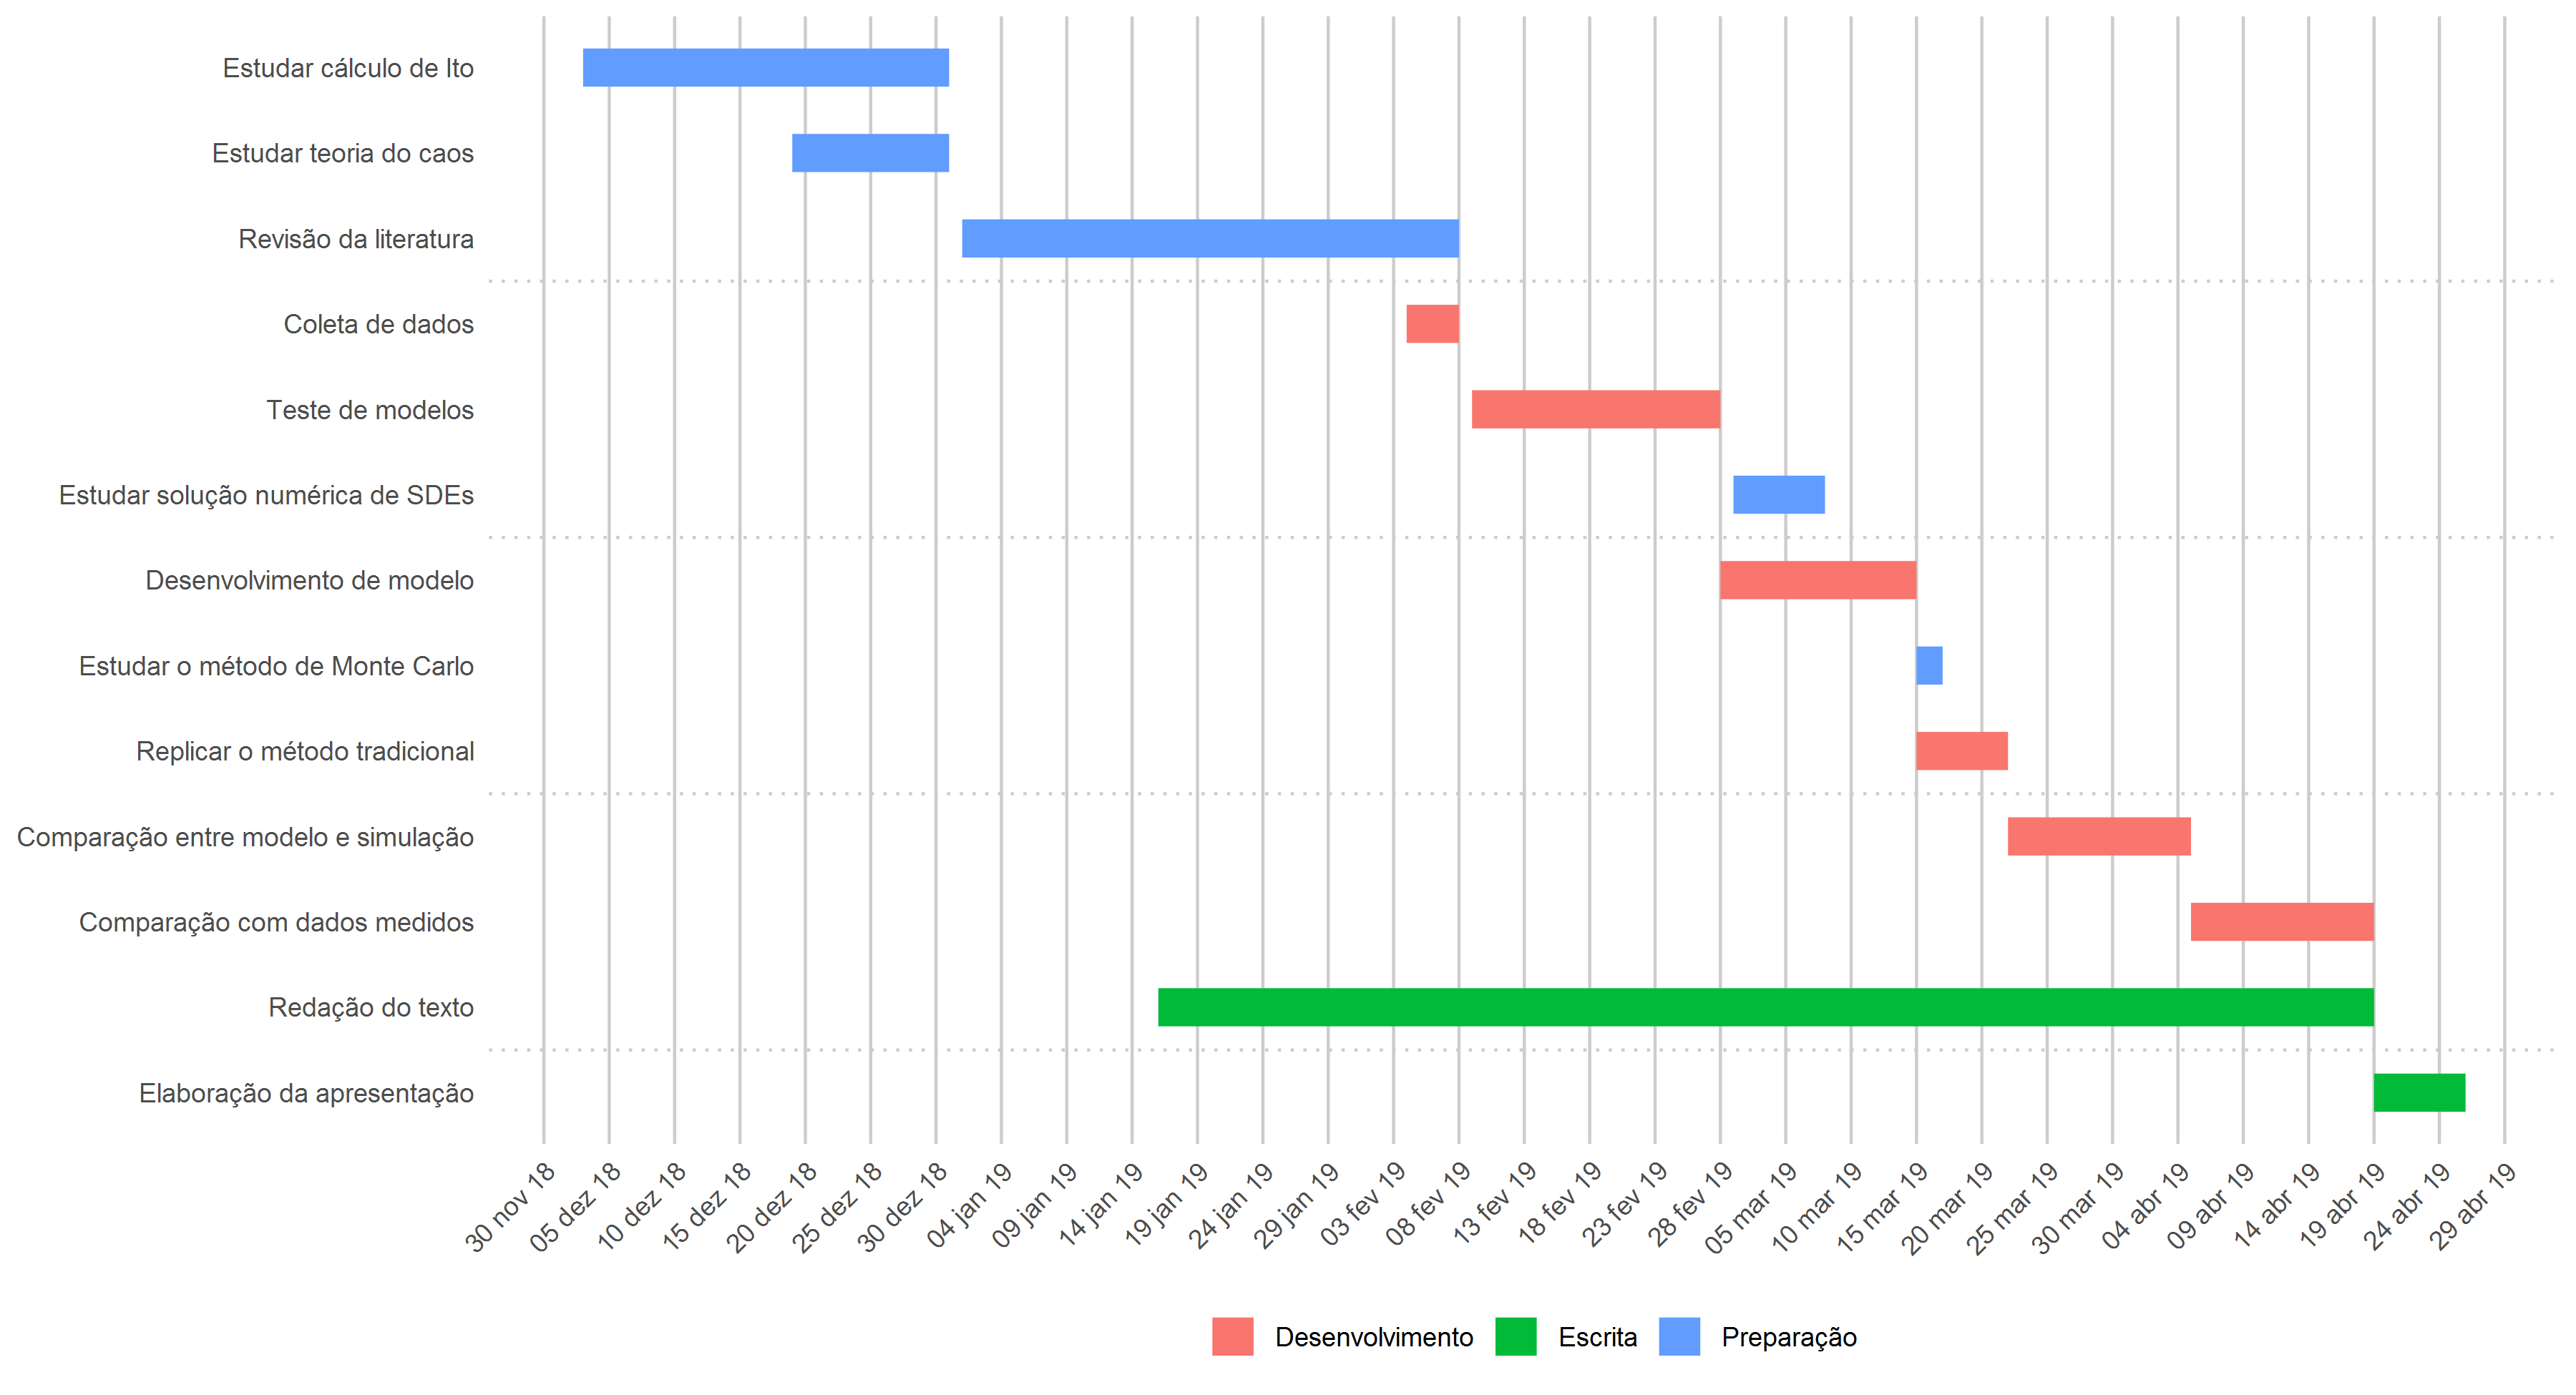
\includegraphics[scale=0.65]{gantt}
%    \caption{Gráfico de Gantt do planejamento das etapas de desenvolvimento do presente trabalho. Fonte: autoria própria.}
%    \centering
%\end{figure}
% ----------------------------------------------------------
% PARTE
% ----------------------------------------------------------
%\part{Preparação da pesquisa}


% 1. Introdução: Aqui vocês têm que convencer o leitor que o tópico de vocês é interessante, que vale a pena ser explorado. Tem que motivar! Trabalhar com econofísica é legal porque... tem problemas 
% paralelos na física... vai me ajudar na minha vida profissional porque...
% 2. Revisão Bibliográfica: Esta seção é para mostrar que vocês leram bastante, estudaram, aprenderam algo novo. Pesquisem tudo que foi feito no tópico de estudo de vocês e contem uma historinha 
% cronológica com este material;     
% 3. Problema: Agora que vocês já convenceram o leitor que o assunto é importante e vocês estão por dentro do assunto, mostrem qual é o problema a ser atacado. Por exemplo: 
% Eu vou aplicar a teoria X para descobrir porque mercados se comportam do jeito Y.
% 4. Metodologia: Para resolver o problema acima, vocês vão dar uma aula sobre o arsenal teórico. Explicar com detalhes o tópico de vocês: catástrofe, multifractal, resonância, etc.
% 5. Cronograma: Bom, feito todo este trabalho, agora é hora de contar pra banca como vocês vão organizar o tempo de vocês para que até julho do ano que vem vocês tenham o TCC2 pronto. 
% Façam um diagrama de Gantt semanal botando metas claras.

% ---
% Capitulo com exemplos de comandos inseridos de arquivo externo 
% ---
%%% abtex2-modelo-include-comandos.tex, v-1.9.6 laurocesar
%% Copyright 2012-2016 by abnTeX2 group at http://www.abntex.net.br/ 
%%
%% This work may be distributed and/or modified under the
%% conditions of the LaTeX Project Public License, either version 1.3
%% of this license or (at your option) any later version.
%% The latest version of this license is in
%%   http://www.latex-project.org/lppl.txt
%% and version 1.3 or later is part of all distributions of LaTeX
%% version 2005/12/01 or later.
%%
%% This work has the LPPL maintenance status `maintained'.
%% 
%% The Current Maintainer of this work is the abnTeX2 team, led
%% by Lauro César Araujo. Further information are available on 
%% http://www.abntex.net.br/
%%
%% This work consists of the files abntex2-modelo-include-comandos.tex
%% and abntex2-modelo-img-marca.pdf
%%

% ---
% Este capítulo, utilizado por diferentes exemplos do abnTeX2, ilustra o uso de
% comandos do abnTeX2 e de LaTeX.
% ---
 
\chapter{Resultados de comandos}\label{cap_exemplos}

\chapterprecis{Isto é uma sinopse de capítulo. A ABNT não traz nenhuma
normatização a respeito desse tipo de resumo, que é mais comum em romances 
e livros técnicos.}\index{sinopse de capítulo}

% ---
\section{Codificação dos arquivos: UTF8}
% ---

A codificação de todos os arquivos do \abnTeX\ é \texttt{UTF8}. É necessário que
você utilize a mesma codificação nos documentos que escrever, inclusive nos
arquivos de base bibliográficas |.bib|.

% ---
\section{Citações diretas}
\label{sec-citacao}
% ---

\index{citações!diretas}Utilize o ambiente \texttt{citacao} para incluir
citações diretas com mais de três linhas:

\begin{citacao}
As citações diretas, no texto, com mais de três linhas, devem ser
destacadas com recuo de 4 cm da margem esquerda, com letra menor que a do texto
utilizado e sem as aspas. No caso de documentos datilografados, deve-se
observar apenas o recuo \cite[5.3]{NBR10520:2002}.
\end{citacao}

Use o ambiente assim:

\begin{verbatim}
\begin{citacao}
As citações diretas, no texto, com mais de três linhas [...] deve-se observar
apenas o recuo \cite[5.3]{NBR10520:2002}.
\end{citacao}
\end{verbatim}

O ambiente \texttt{citacao} pode receber como parâmetro opcional um nome de
idioma previamente carregado nas opções da classe (\autoref{sec-hifenizacao}). Nesse
caso, o texto da citação é automaticamente escrito em itálico e a hifenização é
ajustada para o idioma selecionado na opção do ambiente. Por exemplo:

\begin{verbatim}
\begin{citacao}[english]
Text in English language in italic with correct hyphenation.
\end{citacao}
\end{verbatim}

Tem como resultado:

\begin{citacao}[english]
Text in English language in italic with correct hyphenation.
\end{citacao}

\index{citações!simples}Citações simples, com até três linhas, devem ser
incluídas com aspas. Observe que em \LaTeX as aspas iniciais são diferentes das
finais: ``Amor é fogo que arde sem se ver''.

% ---
\section{Notas de rodapé}
% ---

As notas de rodapé são detalhadas pela NBR 14724:2011 na seção 5.2.1\footnote{As
notas devem ser digitadas ou datilografadas dentro das margens, ficando
separadas do texto por um espaço simples de entre as linhas e por filete de 5
cm, a partir da margem esquerda. Devem ser alinhadas, a partir da segunda linha
da mesma nota, abaixo da primeira letra da primeira palavra, de forma a destacar
o expoente, sem espaço entre elas e com fonte menor
\citeonline[5.2.1]{NBR14724:2011}.}\footnote{Caso uma série de notas sejam
criadas sequencialmente, o \abnTeX\ instrui o \LaTeX\ para que uma vírgula seja
colocada após cada número do expoente que indica a nota de rodapé no corpo do
texto.}\footnote{Verifique se os números do expoente possuem uma vírgula para
dividi-los no corpo do texto.}. 


% ---
\section{Tabelas}
% ---

\index{tabelas}A \autoref{tab-nivinv} é um exemplo de tabela construída em
\LaTeX.

\begin{table}[htb]
\ABNTEXfontereduzida
\caption[Níveis de investigação]{Níveis de investigação.}
\label{tab-nivinv}
\begin{tabular}{p{2.6cm}|p{6.0cm}|p{2.25cm}|p{3.40cm}}
  %\hline
   \textbf{Nível de Investigação} & \textbf{Insumos}  & \textbf{Sistemas de Investigação}  & \textbf{Produtos}  \\
    \hline
    Meta-nível & Filosofia\index{filosofia} da Ciência  & Epistemologia &
    Paradigma  \\
    \hline
    Nível do objeto & Paradigmas do metanível e evidências do nível inferior &
    Ciência  & Teorias e modelos \\
    \hline
    Nível inferior & Modelos e métodos do nível do objeto e problemas do nível inferior & Prática & Solução de problemas  \\
   % \hline
\end{tabular}
\legend{Fonte: \citeonline{van86}}
\end{table}

Já a \autoref{tabela-ibge} apresenta uma tabela criada conforme o padrão do
\citeonline{ibge1993} requerido pelas normas da ABNT para documentos técnicos e
acadêmicos.

\begin{table}[htb]
\IBGEtab{%
  \caption{Um Exemplo de tabela alinhada que pode ser longa
  ou curta, conforme padrão IBGE.}%
  \label{tabela-ibge}
}{%
  \begin{tabular}{ccc}
  \toprule
   Nome & Nascimento & Documento \\
  \midrule \midrule
   Maria da Silva & 11/11/1111 & 111.111.111-11 \\
  \midrule 
   João Souza & 11/11/2111 & 211.111.111-11 \\
  \midrule 
   Laura Vicuña & 05/04/1891 & 3111.111.111-11 \\
  \bottomrule
\end{tabular}%
}{%
  \fonte{Produzido pelos autores.}%
  \nota{Esta é uma nota, que diz que os dados são baseados na
  regressão linear.}%
  \nota[Anotações]{Uma anotação adicional, que pode ser seguida de várias
  outras.}%
  }
\end{table}


% ---
\section{Figuras}
% ---

\index{figuras}Figuras podem ser criadas diretamente em \LaTeX,
como o exemplo da \autoref{fig_circulo}.

\begin{figure}[htb]
	\caption{\label{fig_circulo}A delimitação do espaço}
	\begin{center}
	    \setlength{\unitlength}{5cm}
		\begin{picture}(1,1)
		\put(0,0){\line(0,1){1}}
		\put(0,0){\line(1,0){1}}
		\put(0,0){\line(1,1){1}}
		\put(0,0){\line(1,2){.5}}
		\put(0,0){\line(1,3){.3333}}
		\put(0,0){\line(1,4){.25}}
		\put(0,0){\line(1,5){.2}}
		\put(0,0){\line(1,6){.1667}}
		\put(0,0){\line(2,1){1}}
		\put(0,0){\line(2,3){.6667}}
		\put(0,0){\line(2,5){.4}}
		\put(0,0){\line(3,1){1}}
		\put(0,0){\line(3,2){1}}
		\put(0,0){\line(3,4){.75}}
		\put(0,0){\line(3,5){.6}}
		\put(0,0){\line(4,1){1}}
		\put(0,0){\line(4,3){1}}
		\put(0,0){\line(4,5){.8}}
		\put(0,0){\line(5,1){1}}
		\put(0,0){\line(5,2){1}}
		\put(0,0){\line(5,3){1}}
		\put(0,0){\line(5,4){1}}
		\put(0,0){\line(5,6){.8333}}
		\put(0,0){\line(6,1){1}}
		\put(0,0){\line(6,5){1}}
		\end{picture}
	\end{center}
	\legend{Fonte: os autores}
\end{figure}

Ou então figuras podem ser incorporadas de arquivos externos, como é o caso da
\autoref{fig_grafico}. Se a figura que ser incluída se tratar de um diagrama, um
gráfico ou uma ilustração que você mesmo produza, priorize o uso de imagens
vetoriais no formato PDF. Com isso, o tamanho do arquivo final do trabalho será
menor, e as imagens terão uma apresentação melhor, principalmente quando
impressas, uma vez que imagens vetorias são perfeitamente escaláveis para
qualquer dimensão. Nesse caso, se for utilizar o Microsoft Excel para produzir
gráficos, ou o Microsoft Word para produzir ilustrações, exporte-os como PDF e
os incorpore ao documento conforme o exemplo abaixo. No entanto, para manter a
coerência no uso de software livre (já que você está usando \LaTeX e \abnTeX),
teste a ferramenta \textsf{InkScape}\index{InkScape}
(\url{http://inkscape.org/}). Ela é uma excelente opção de código-livre para
produzir ilustrações vetoriais, similar ao CorelDraw\index{CorelDraw} ou ao Adobe
Illustrator\index{Adobe Illustrator}. De todo modo, caso não seja possível
utilizar arquivos de imagens como PDF, utilize qualquer outro formato, como
JPEG, GIF, BMP, etc. Nesse caso, você pode tentar aprimorar as imagens
incorporadas com o software livre \textsf{Gimp}\index{Gimp}
(\url{http://www.gimp.org/}). Ele é uma alternativa livre ao Adobe
Photoshop\index{Adobe Photoshop}.

\begin{figure}[htb]
	\caption{\label{fig_grafico}Gráfico produzido em Excel e salvo como PDF}
	\begin{center}
	    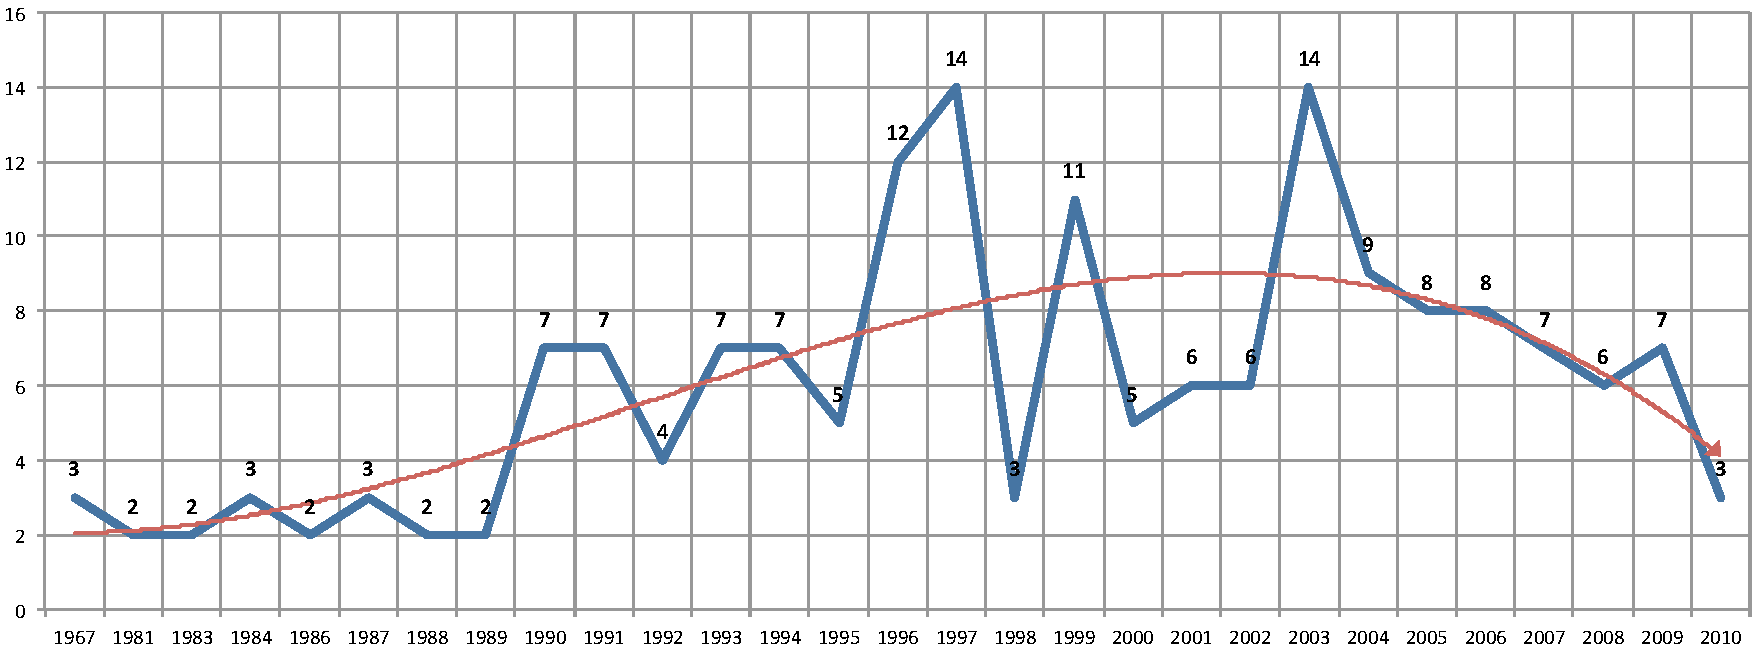
\includegraphics[scale=0.5]{abntex2-modelo-img-grafico.pdf}
	\end{center}
	\legend{Fonte: \citeonline[p. 24]{araujo2012}}
\end{figure}

% ---
\subsection{Figuras em \emph{minipages}}
% ---

\emph{Minipages} são usadas para inserir textos ou outros elementos em quadros
com tamanhos e posições controladas. Veja o exemplo da
\autoref{fig_minipage_imagem1} e da \autoref{fig_minipage_grafico2}.

\begin{figure}[htb]
 \label{teste}
 \centering
  \begin{minipage}{0.4\textwidth}
    \centering
    \caption{Imagem 1 da minipage} \label{fig_minipage_imagem1}
    
\includegraphics[scale=0.9]{abntex2-modelo-img-marca.pdf}
    \legend{Fonte: Produzido pelos autores}
  \end{minipage}
  \hfill
  \begin{minipage}{0.4\textwidth}
    \centering
    \caption{Grafico 2 da minipage} \label{fig_minipage_grafico2}
    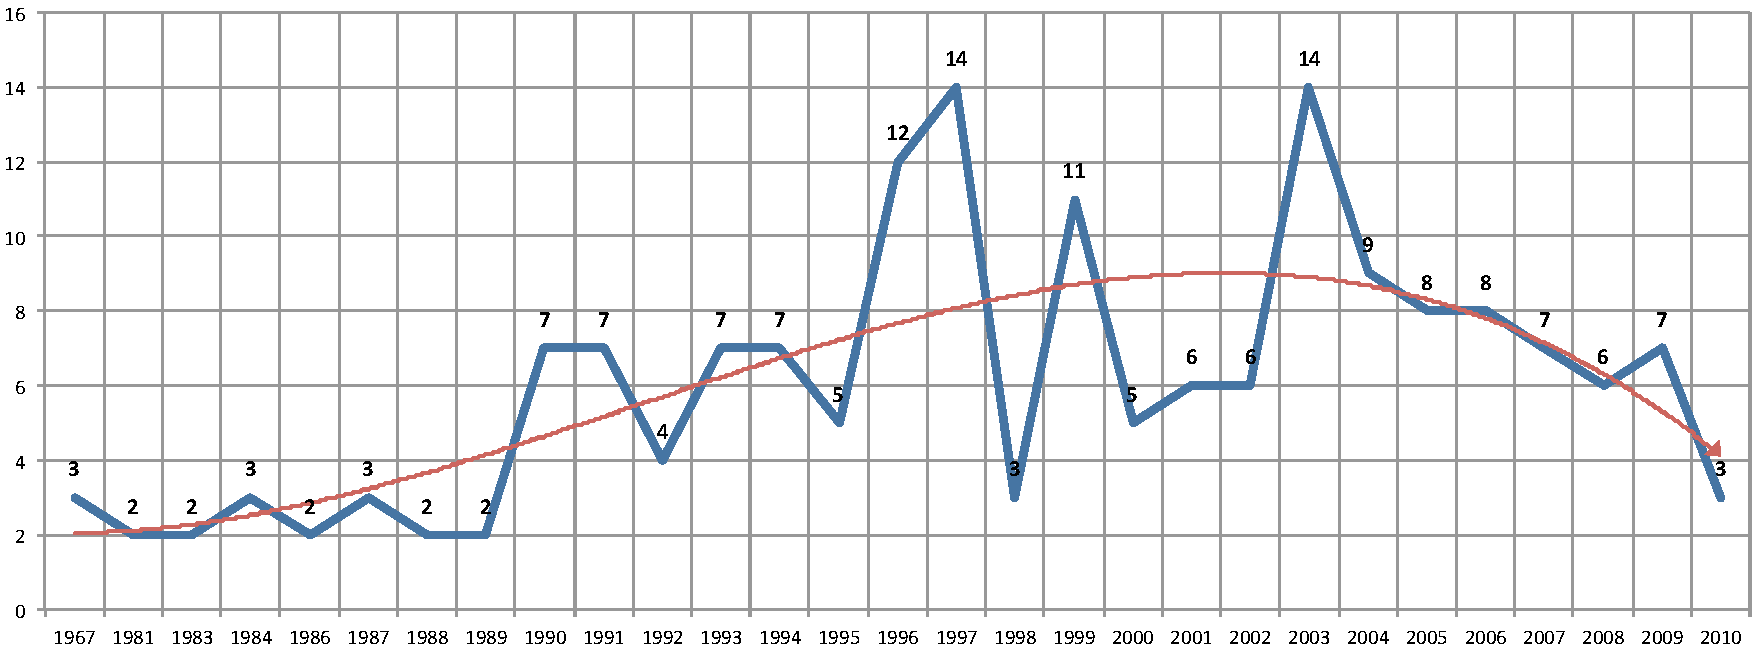
\includegraphics[scale=0.2]{abntex2-modelo-img-grafico.pdf}
    \legend{Fonte: \citeonline[p. 24]{araujo2012}}
  \end{minipage}
\end{figure}

Observe que, segundo a \citeonline[seções 4.2.1.10 e 5.8]{NBR14724:2011}, as
ilustrações devem sempre ter numeração contínua e única em todo o documento:

\begin{citacao}
Qualquer que seja o tipo de ilustração, sua identificação aparece na parte
superior, precedida da palavra designativa (desenho, esquema, fluxograma,
fotografia, gráfico, mapa, organograma, planta, quadro, retrato, figura,
imagem, entre outros), seguida de seu número de ordem de ocorrência no texto,
em algarismos arábicos, travessão e do respectivo título. Após a ilustração, na
parte inferior, indicar a fonte consultada (elemento obrigatório, mesmo que
seja produção do próprio autor), legenda, notas e outras informações
necessárias à sua compreensão (se houver). A ilustração deve ser citada no
texto e inserida o mais próximo possível do trecho a que se
refere. \cite[seções 5.8]{NBR14724:2011}
\end{citacao}

% ---
\section{Expressões matemáticas}
% ---

\index{expressões matemáticas}Use o ambiente \texttt{equation} para escrever
expressões matemáticas numeradas:

\begin{equation}
  \forall x \in X, \quad \exists \: y \leq \epsilon
\end{equation}

Escreva expressões matemáticas entre \$ e \$, como em $ \lim_{x \to \infty}
\exp(-x) = 0 $, para que fiquem na mesma linha.

Também é possível usar colchetes para indicar o início de uma expressão
matemática que não é numerada.

\[
\left|\sum_{i=1}^n a_ib_i\right|
\le
\left(\sum_{i=1}^n a_i^2\right)^{1/2}
\left(\sum_{i=1}^n b_i^2\right)^{1/2}
\]

Consulte mais informações sobre expressões matemáticas em
\url{https://github.com/abntex/abntex2/wiki/Referencias}.

% ---
\section{Enumerações: alíneas e subalíneas}
% ---

\index{alíneas}\index{subalíneas}\index{incisos}Quando for necessário enumerar
os diversos assuntos de uma seção que não possua título, esta deve ser
subdividida em alíneas \cite[4.2]{NBR6024:2012}:

\begin{alineas}

  \item os diversos assuntos que não possuam título próprio, dentro de uma mesma
  seção, devem ser subdivididos em alíneas; 
  
  \item o texto que antecede as alíneas termina em dois pontos;
  \item as alíneas devem ser indicadas alfabeticamente, em letra minúscula,
  seguida de parêntese. Utilizam-se letras dobradas, quando esgotadas as
  letras do alfabeto;

  \item as letras indicativas das alíneas devem apresentar recuo em relação à
  margem esquerda;

  \item o texto da alínea deve começar por letra minúscula e terminar em
  ponto-e-vírgula, exceto a última alínea que termina em ponto final;

  \item o texto da alínea deve terminar em dois pontos, se houver subalínea;

  \item a segunda e as seguintes linhas do texto da alínea começa sob a
  primeira letra do texto da própria alínea;
  
  \item subalíneas \cite[4.3]{NBR6024:2012} devem ser conforme as alíneas a
  seguir:

  \begin{alineas}
     \item as subalíneas devem começar por travessão seguido de espaço;

     \item as subalíneas devem apresentar recuo em relação à alínea;

     \item o texto da subalínea deve começar por letra minúscula e terminar em
     ponto-e-vírgula. A última subalínea deve terminar em ponto final, se não
     houver alínea subsequente;

     \item a segunda e as seguintes linhas do texto da subalínea começam sob a
     primeira letra do texto da própria subalínea.
  \end{alineas}
  
  \item no \abnTeX\ estão disponíveis os ambientes \texttt{incisos} e
  \texttt{subalineas}, que em suma são o mesmo que se criar outro nível de
  \texttt{alineas}, como nos exemplos à seguir:
  
  \begin{incisos}
    \item \textit{Um novo inciso em itálico};
  \end{incisos}
  
  \item Alínea em \textbf{negrito}:
  
  \begin{subalineas}
    \item \textit{Uma subalínea em itálico};
    \item \underline{\textit{Uma subalínea em itálico e sublinhado}}; 
  \end{subalineas}
  
  \item Última alínea com \emph{ênfase}.
  
\end{alineas}

% ---
\section{Espaçamento entre parágrafos e linhas}
% ---

\index{espaçamento!dos parágrafos}O tamanho do parágrafo, espaço entre a margem
e o início da frase do parágrafo, é definido por:

\begin{verbatim}
   \setlength{\parindent}{1.3cm}
\end{verbatim}

\index{espaçamento!do primeiro parágrafo}Por padrão, não há espaçamento no
primeiro parágrafo de cada início de divisão do documento
(\autoref{sec-divisoes}). Porém, você pode definir que o primeiro parágrafo
também seja indentado, como é o caso deste documento. Para isso, apenas inclua o
pacote \textsf{indentfirst} no preâmbulo do documento:

\begin{verbatim}
   \usepackage{indentfirst}      % Indenta o primeiro parágrafo de cada seção.
\end{verbatim}

\index{espaçamento!entre os parágrafos}O espaçamento entre um parágrafo e outro
pode ser controlado por meio do comando:

\begin{verbatim}
  \setlength{\parskip}{0.2cm}  % tente também \onelineskip
\end{verbatim}

\index{espaçamento!entre as linhas}O controle do espaçamento entre linhas é
definido por:

\begin{verbatim}
  \OnehalfSpacing       % espaçamento um e meio (padrão); 
  \DoubleSpacing        % espaçamento duplo
  \SingleSpacing        % espaçamento simples	
\end{verbatim}

Para isso, também estão disponíveis os ambientes:

\begin{verbatim}
  \begin{SingleSpace} ...\end{SingleSpace}
  \begin{Spacing}{hfactori} ... \end{Spacing}
  \begin{OnehalfSpace} ... \end{OnehalfSpace}
  \begin{OnehalfSpace*} ... \end{OnehalfSpace*}
  \begin{DoubleSpace} ... \end{DoubleSpace}
  \begin{DoubleSpace*} ... \end{DoubleSpace*} 
\end{verbatim}

Para mais informações, consulte \citeonline[p. 47-52 e 135]{memoir}.

% ---
\section{Inclusão de outros arquivos}\label{sec-include}
% ---

É uma boa prática dividir o seu documento em diversos arquivos, e não
apenas escrever tudo em um único. Esse recurso foi utilizado neste
documento. Para incluir diferentes arquivos em um arquivo principal,
de modo que cada arquivo incluído fique em uma página diferente, utilize o
comando:

\begin{verbatim}
   \include{documento-a-ser-incluido}      % sem a extensão .tex
\end{verbatim}

Para incluir documentos sem quebra de páginas, utilize:

\begin{verbatim}
   \input{documento-a-ser-incluido}      % sem a extensão .tex
\end{verbatim}

% ---
\section{Compilar o documento \LaTeX}
% ---

Geralmente os editores \LaTeX, como o
TeXlipse\footnote{\url{http://texlipse.sourceforge.net/}}, o
Texmaker\footnote{\url{http://www.xm1math.net/texmaker/}}, entre outros,
compilam os documentos automaticamente, de modo que você não precisa se
preocupar com isso.

No entanto, você pode compilar os documentos \LaTeX usando os seguintes
comandos, que devem ser digitados no \emph{Prompt de Comandos} do Windows ou no
\emph{Terminal} do Mac ou do Linux:

\begin{verbatim}
   pdflatex ARQUIVO_PRINCIPAL.tex
   bibtex ARQUIVO_PRINCIPAL.aux
   makeindex ARQUIVO_PRINCIPAL.idx 
   makeindex ARQUIVO_PRINCIPAL.nlo -s nomencl.ist -o ARQUIVO_PRINCIPAL.nls
   pdflatex ARQUIVO_PRINCIPAL.tex
   pdflatex ARQUIVO_PRINCIPAL.tex
\end{verbatim}

% ---
\section{Remissões internas}
% ---

Ao nomear a \autoref{tab-nivinv} e a \autoref{fig_circulo}, apresentamos um
exemplo de remissão interna, que também pode ser feita quando indicamos o
\autoref{cap_exemplos}, que tem o nome \emph{\nameref{cap_exemplos}}. O número
do capítulo indicado é \ref{cap_exemplos}, que se inicia à
\autopageref{cap_exemplos}\footnote{O número da página de uma remissão pode ser
obtida também assim:
\pageref{cap_exemplos}.}.
Veja a \autoref{sec-divisoes} para outros exemplos de remissões internas entre
seções, subseções e subsubseções.

O código usado para produzir o texto desta seção é:

\begin{verbatim}
Ao nomear a \autoref{tab-nivinv} e a \autoref{fig_circulo}, apresentamos um
exemplo de remissão interna, que também pode ser feita quando indicamos o
\autoref{cap_exemplos}, que tem o nome \emph{\nameref{cap_exemplos}}. O número
do capítulo indicado é \ref{cap_exemplos}, que se inicia à
\autopageref{cap_exemplos}\footnote{O número da página de uma remissão pode ser
obtida também assim:
\pageref{cap_exemplos}.}.
Veja a \autoref{sec-divisoes} para outros exemplos de remissões internas entre
seções, subseções e subsubseções.
\end{verbatim}

% ---
\section{Divisões do documento: seção}\label{sec-divisoes}
% ---

Esta seção testa o uso de divisões de documentos. Esta é a
\autoref{sec-divisoes}. Veja a \autoref{sec-divisoes-subsection}.

\subsection{Divisões do documento: subseção}\label{sec-divisoes-subsection}

Isto é uma subseção. Veja a \autoref{sec-divisoes-subsubsection}, que é uma
\texttt{subsubsection} do \LaTeX, mas é impressa chamada de ``subseção'' porque
no Português não temos a palavra ``subsubseção''.

\subsubsection{Divisões do documento: subsubseção}
\label{sec-divisoes-subsubsection}

Isto é uma subsubseção.

\subsubsection{Divisões do documento: subsubseção}

Isto é outra subsubseção.

\subsection{Divisões do documento: subseção}\label{sec-exemplo-subsec}

Isto é uma subseção.

\subsubsection{Divisões do documento: subsubseção}

Isto é mais uma subsubseção da \autoref{sec-exemplo-subsec}.


\subsubsubsection{Esta é uma subseção de quinto
nível}\label{sec-exemplo-subsubsubsection}

Esta é uma seção de quinto nível. Ela é produzida com o seguinte comando:

\begin{verbatim}
\subsubsubsection{Esta é uma subseção de quinto
nível}\label{sec-exemplo-subsubsubsection}
\end{verbatim}

\subsubsubsection{Esta é outra subseção de quinto nível}\label{sec-exemplo-subsubsubsection-outro}

Esta é outra seção de quinto nível.


\paragraph{Este é um parágrafo numerado}\label{sec-exemplo-paragrafo}

Este é um exemplo de parágrafo nomeado. Ele é produzida com o comando de
parágrafo:

\begin{verbatim}
\paragraph{Este é um parágrafo nomeado}\label{sec-exemplo-paragrafo}
\end{verbatim}

A numeração entre parágrafos numeradaos e subsubsubseções são contínuas.

\paragraph{Esta é outro parágrafo numerado}\label{sec-exemplo-paragrafo-outro}

Esta é outro parágrafo nomeado.

% ---
\section{Este é um exemplo de nome de seção longo. Ele deve estar
alinhado à esquerda e a segunda e demais linhas devem iniciar logo abaixo da
primeira palavra da primeira linha}
% ---

Isso atende à norma \citeonline[seções de 5.2.2 a 5.2.4]{NBR14724:2011} 
 e \citeonline[seções de 3.1 a 3.8]{NBR6024:2012}.

% ---
\section{Diferentes idiomas e hifenizações}
\label{sec-hifenizacao}
% ---

Para usar hifenizações de diferentes idiomas, inclua nas opções do documento o
nome dos idiomas que o seu texto contém. Por exemplo (para melhor
visualização, as opções foram quebras em diferentes linhas):

\begin{verbatim}
\documentclass[
	12pt,
	openright,
	twoside,
	a4paper,
	english,
	french,
	spanish,
	brazil
	]{abntex2}
\end{verbatim}

O idioma português-brasileiro (\texttt{brazil}) é incluído automaticamente pela
classe \textsf{abntex2}. Porém, mesmo assim a opção \texttt{brazil} deve ser
informada como a última opção da classe para que todos os pacotes reconheçam o
idioma. Vale ressaltar que a última opção de idioma é a utilizada por padrão no
documento. Desse modo, caso deseje escrever um texto em inglês que tenha
citações em português e em francês, você deveria usar o preâmbulo como abaixo:

\begin{verbatim}
\documentclass[
	12pt,
	openright,
	twoside,
	a4paper,
	french,
	brazil,
	english
	]{abntex2}
\end{verbatim}

A lista completa de idiomas suportados, bem como outras opções de hifenização,
estão disponíveis em \citeonline[p.~5-6]{babel}.

Exemplo de hifenização em inglês\footnote{Extraído de:
\url{http://en.wikibooks.org/wiki/LaTeX/Internationalization}}:

\begin{otherlanguage*}{english}
\textit{Text in English language. This environment switches all language-related
definitions, like the language specific names for figures, tables etc. to the other
language. The starred version of this environment typesets the main text
according to the rules of the other language, but keeps the language specific
string for ancillary things like figures, in the main language of the document.
The environment hyphenrules switches only the hyphenation patterns used; it can
also be used to disallow hyphenation by using the language name
`nohyphenation'.}
\end{otherlanguage*}

Exemplo de hifenização em francês\footnote{Extraído de:
\url{http://bigbrowser.blog.lemonde.fr/2013/02/17/tu-ne-tweeteras-point-le-vatican-interdit-aux-cardinaux-de-tweeter-pendant-le-conclave/}}:

\begin{otherlanguage*}{french}
\textit{Texte en français. Pas question que Twitter ne vienne faire une
concurrence déloyale à la traditionnelle fumée blanche qui marque l'élection
d'un nouveau pape. Pour éviter toute fuite précoce, le Vatican a donc pris un
peu d'avance, et a déjà interdit aux cardinaux qui prendront part au vote
d'utiliser le réseau social, selon Catholic News Service. Une mesure valable
surtout pour les neuf cardinaux – sur les 117 du conclave – pratiquants très
actifs de Twitter, qui auront interdiction pendant toute la période de se
connecter à leur compte.}
\end{otherlanguage*}

Pequeno texto em espanhol\footnote{Extraído de:
\url{http://internacional.elpais.com/internacional/2013/02/17/actualidad/1361102009_913423.html}}:

\foreignlanguage{spanish}{\textit{Decenas de miles de personas ovacionan al pontífice en su
penúltimo ángelus dominical, el primero desde que anunciase su renuncia. El Papa se
centra en la crítica al materialismo}}.

O idioma geral do texto por ser alterado como no exemplo seguinte:

\begin{verbatim}
  \selectlanguage{english}
\end{verbatim}

Isso altera automaticamente a hifenização e todos os nomes constantes de
referências do documento para o idioma inglês. Consulte o manual da classe
\cite{abntex2classe} para obter orientações adicionais sobre internacionalização de
documentos produzidos com \abnTeX.

A \autoref{sec-citacao} descreve o ambiente \texttt{citacao} que pode receber
como parâmetro um idioma a ser usado na citação.

% ---
\section{Consulte o manual da classe \textsf{abntex2}}
% ---

Consulte o manual da classe \textsf{abntex2} \cite{abntex2classe} para uma
referência completa das macros e ambientes disponíveis. 

Além disso, o manual possui informações adicionais sobre as normas ABNT
observadas pelo \abnTeX\ e considerações sobre eventuais requisitos específicos
não atendidos, como o caso da \citeonline[seção 5.2.2]{NBR14724:2011}, que
especifica o espaçamento entre os capítulos e o início do texto, regra
propositalmente não atendida pelo presente modelo.

% ---
\section{Referências bibliográficas}
% ---

A formatação das referências bibliográficas conforme as regras da ABNT são um
dos principais objetivos do \abnTeX. Consulte os manuais
\citeonline{abntex2cite} e \citeonline{abntex2cite-alf} para obter informações
sobre como utilizar as referências bibliográficas.

%-
\subsection{Acentuação de referências bibliográficas}
%-

Normalmente não há problemas em usar caracteres acentuados em arquivos
bibliográficos (\texttt{*.bib}). Porém, como as regras da ABNT fazem uso quase
abusivo da conversão para letras maiúsculas, é preciso observar o modo como se
escreve os nomes dos autores. Na ~\autoref{tabela-acentos} você encontra alguns
exemplos das conversões mais importantes. Preste atenção especial para `ç' e `í'
que devem estar envoltos em chaves. A regra geral é sempre usar a acentuação
neste modo quando houver conversão para letras maiúsculas.

\begin{table}[htbp]
\caption{Tabela de conversão de acentuação.}
\label{tabela-acentos}

\begin{center}
\begin{tabular}{ll}\hline\hline
acento & \textsf{bibtex}\\
à á ã & \verb+\`a+ \verb+\'a+ \verb+\~a+\\
í & \verb+{\'\i}+\\
ç & \verb+{\c c}+\\
\hline\hline
\end{tabular}
\end{center}
\end{table}


% ---
\section{Precisa de ajuda?}
% ---

Consulte a FAQ com perguntas frequentes e comuns no portal do \abnTeX:
\url{https://github.com/abntex/abntex2/wiki/FAQ}.

Inscreva-se no grupo de usuários \LaTeX:
\url{http://groups.google.com/group/latex-br}, tire suas dúvidas e ajude
outros usuários.

Participe também do grupo de desenvolvedores do \abnTeX:
\url{http://groups.google.com/group/abntex2} e faça sua contribuição à
ferramenta.

% ---
\section{Você pode ajudar?}
% ---

Sua contribuição é muito importante! Você pode ajudar na divulgação, no
desenvolvimento e de várias outras formas. Veja como contribuir com o \abnTeX\
em \url{https://github.com/abntex/abntex2/wiki/Como-Contribuir}.

% ---
\section{Quer customizar os modelos do \abnTeX\ para sua instituição ou
universidade?}
% ---

Veja como customizar o \abnTeX\ em:
\url{https://github.com/abntex/abntex2/wiki/ComoCustomizar}.


% ---

% ----------------------------------------------------------
% PARTE
% ----------------------------------------------------------
%\part{Referenciais teóricos}
% ----------------------------------------------------------

% ---
% Capitulo de revisão de literatura
% ---
%\chapter{Lorem ipsum dolor sit amet}
% ---

% ---
%\section{Aliquam vestibulum fringilla lorem}
% ---

%\lipsum[1]

%\lipsum[2-3]

% ----------------------------------------------------------
% PARTE
% ----------------------------------------------------------
%\part{Resultados}
% ----------------------------------------------------------

% ---
% primeiro capitulo de Resultados
% ---
%\chapter{Lectus lobortis condimentum}
% ---

% ---
%\section{Vestibulum ante ipsum primis in faucibus orci luctus et ultrices posuere cubilia Curae}
% ---

%\lipsum[21-22]

% ---
% segundo capitulo de Resultados
% ---
%\chapter{Nam sed tellus sit amet lectus urna ullamcorper tristique interdum elementum}
% ---

% ---
%\section{Pellentesque sit amet pede ac sem eleifend consectetuer}
% ---

%\lipsum[24]

% ----------------------------------------------------------
% Finaliza a parte no bookmark do PDF
% para que se inicie o bookmark na raiz
% e adiciona espaço de parte no Sumário
% ----------------------------------------------------------
%\phantompart

% ---
% Conclusão
% ---
%\chapter{Conclusão}
% ---

%\lipsum[31-33]

% ----------------------------------------------------------
% ELEMENTOS PÓS-TEXTUAIS
% ----------------------------------------------------------
%\postextual
% ----------------------------------------------------------

% ----------------------------------------------------------
% Referências bibliográficas
% ----------------------------------------------------------
\bibliography{abntex2-modelo-references}

% ----------------------------------------------------------
% Glossário
% ----------------------------------------------------------
%
% Consulte o manual da classe abntex2 para orientações sobre o glossário.
%
%\glossary

% ----------------------------------------------------------
% Apêndices
% ----------------------------------------------------------

% ---
% Inicia os apêndices
% ---
%\begin{apendicesenv}
%
%% Imprime uma página indicando o início dos apêndices
%\partapendices
%
%% ----------------------------------------------------------
%\chapter{Quisque libero justo}
%% ----------------------------------------------------------
%
%\lipsum[50]
%
%% ---
%{Nullam elementum urna vel imperdiet sodales elit ipsum pharetra ligula
%ac pretium ante justo a nulla curabitur tristique arcu eu metus}
%% ----------------------------------------------------------
%\lipsum[55-57]
%
%\end{apendicesenv}
% ---


% ----------------------------------------------------------
% Anexos
% ----------------------------------------------------------

% ---
% Inicia os anexos
% ---
%\begin{anexosenv}

% Imprime uma página indicando o início dos anexos
%\partanexos

% ---
%\chapter{Morbi ultrices rutrum lorem.}
% ---
%\lipsum[30]

% ---
%\chapter{Cras non urna sed feugiat cum sociis natoque penatibus et magnis dis parturient montes nascetur ridiculus mus}
% ---

%\lipsum[31]

% ---
%\chapter{Fusce facilisis lacinia dui}
% ---

%\lipsum[32]

%\end{anexosenv}

%---------------------------------------------------------------------
% INDICE REMISSIVO
%---------------------------------------------------------------------
\phantompart
\printindex
%---------------------------------------------------------------------

\end{document}
